% =====================================================================
%  Trabajo Terminal 2026-B136 — ESCOM / IPN
%  "Prototipo de un sistema web para la gestión de expedientes
%   digitales y actividad procesal de un despacho legal,
%   con servicios de integridad y no repudio."
%
%  Autores : Eduardo Alonso Sánchez · Hatziry Vitales Herrera
%  Directora: Sandra Díaz Santiago
%
%  Compilar con LuaLaTeX:
%      latexmk -lualatex main.tex      (recomendado)
%  o manualmente:
%      lualatex main → biber main → makeglossaries main → lualatex×2
% =====================================================================
\documentclass[12pt,letterpaper,oneside]{report}

% =====================================================================
%  preamble.tex — Configuración global del documento
%  Trabajo Terminal 2026-B136 — ESCOM / IPN
%  Motor recomendado: LuaLaTeX  (lualatex / latexmk -lualatex)
% =====================================================================

% ---------- Idioma y codificación -----------------------------------
\usepackage[spanish,es-tabla,es-noindentfirst,es-nosectiondot]{babel}
\usepackage{csquotes}

% ---------- Tipografía (fontspec, LuaLaTeX) -------------------------
% Times New Roman en TODO el documento (cuerpo, títulos, portada,
% encabezados), igual que el documento Word original. Solo el código
% conserva una fuente monoespaciada (legibilidad/alineación).
\usepackage{fontspec}
\setmainfont{Times New Roman}      % cuerpo
\setsansfont{Times New Roman}      % títulos y encabezados (todo Times)
\setmonofont[Scale=0.88]{DejaVu Sans Mono} % solo bloques de código
\usepackage{microtype}             % refinamiento tipográfico

% ---------- Geometría y espaciado -----------------------------------
\usepackage[letterpaper,top=2.3cm,bottom=2.3cm,left=2.5cm,right=2.3cm]{geometry}
\usepackage{setspace}
\singlespacing                     % interlineado sencillo (igual que el Word)
\usepackage{ragged2e}
\usepackage[hyphens]{url}

% ---------- Matemáticas ---------------------------------------------
\usepackage{amsmath,amssymb,mathtools}

% ---------- Glifos Unicode ausentes en TeX Gyre (super/subíndices,
%            flechas) → se componen en modo matemático ---------------
\usepackage{newunicodechar}
\newunicodechar{⁰}{\ensuremath{^{0}}}\newunicodechar{¹}{\ensuremath{^{1}}}
\newunicodechar{²}{\ensuremath{^{2}}}\newunicodechar{³}{\ensuremath{^{3}}}
\newunicodechar{⁴}{\ensuremath{^{4}}}\newunicodechar{⁵}{\ensuremath{^{5}}}
\newunicodechar{⁶}{\ensuremath{^{6}}}\newunicodechar{⁷}{\ensuremath{^{7}}}
\newunicodechar{⁸}{\ensuremath{^{8}}}\newunicodechar{⁹}{\ensuremath{^{9}}}
\newunicodechar{⁺}{\ensuremath{^{+}}}\newunicodechar{⁻}{\ensuremath{^{-}}}
\newunicodechar{ⁿ}{\ensuremath{^{n}}}
\newunicodechar{₀}{\ensuremath{_{0}}}\newunicodechar{₁}{\ensuremath{_{1}}}
\newunicodechar{₂}{\ensuremath{_{2}}}\newunicodechar{₃}{\ensuremath{_{3}}}
\newunicodechar{₄}{\ensuremath{_{4}}}\newunicodechar{₅}{\ensuremath{_{5}}}
\newunicodechar{₆}{\ensuremath{_{6}}}\newunicodechar{₇}{\ensuremath{_{7}}}
\newunicodechar{₈}{\ensuremath{_{8}}}\newunicodechar{₉}{\ensuremath{_{9}}}
\newunicodechar{₊}{\ensuremath{_{+}}}\newunicodechar{₋}{\ensuremath{_{-}}}
\newunicodechar{↔}{\ensuremath{\leftrightarrow}}
\newunicodechar{→}{\ensuremath{\rightarrow}}\newunicodechar{←}{\ensuremath{\leftarrow}}
\newunicodechar{⇒}{\ensuremath{\Rightarrow}}\newunicodechar{⇔}{\ensuremath{\Leftrightarrow}}
\newunicodechar{≤}{\ensuremath{\leq}}\newunicodechar{≥}{\ensuremath{\geq}}
\newunicodechar{≈}{\ensuremath{\approx}}\newunicodechar{≠}{\ensuremath{\neq}}
\newunicodechar{×}{\ensuremath{\times}}\newunicodechar{∈}{\ensuremath{\in}}
\newunicodechar{‖}{\ensuremath{\Vert}}\newunicodechar{∥}{\ensuremath{\Vert}}

% ---------- Gráficos y figuras --------------------------------------
\usepackage{graphicx}
\graphicspath{{figures/}}
\usepackage{float}
\usepackage{subcaption}
\usepackage[font=small,labelfont=bf,margin=1cm]{caption}

% ---------- Tablas ---------------------------------------------------
\usepackage{booktabs}
\usepackage{longtable}
\usepackage{tabularx}
\usepackage{array}
\usepackage{multirow}
\usepackage{makecell}
\renewcommand{\arraystretch}{1.15}
% Columnas tipo X con alineaciones
\newcolumntype{L}[1]{>{\raggedright\arraybackslash}p{#1}}
\newcolumntype{C}[1]{>{\centering\arraybackslash}p{#1}}
\newcolumntype{R}[1]{>{\raggedleft\arraybackslash}p{#1}}

% ---------- Listas ---------------------------------------------------
\usepackage{enumitem}
\setlist{itemsep=2pt,topsep=4pt}

% ---------- Código ---------------------------------------------------
\usepackage{listings}
\usepackage{xcolor}
\definecolor{codebg}{HTML}{F6F8FA}
\definecolor{codekw}{HTML}{0F62FE}
\definecolor{codecmt}{HTML}{6A737D}
\definecolor{codestr}{HTML}{0A7D33}
\definecolor{ipnvino}{HTML}{6B1E3C}   % guinda IPN
\lstset{
  basicstyle=\ttfamily\small,
  backgroundcolor=\color{codebg},
  keywordstyle=\color{codekw}\bfseries,
  commentstyle=\color{codecmt}\itshape,
  stringstyle=\color{codestr},
  numberstyle=\tiny\color{codecmt},
  numbers=left,numbersep=8pt,
  frame=single,rulecolor=\color{codecmt!30},
  breaklines=true,showstringspaces=false,
  tabsize=2,captionpos=b,
  literate={á}{{\'a}}1 {é}{{\'e}}1 {í}{{\'i}}1 {ó}{{\'o}}1 {ú}{{\'u}}1
           {ñ}{{\~n}}1 {Á}{{\'A}}1 {É}{{\'E}}1 {Í}{{\'I}}1 {Ó}{{\'O}}1
           {Ú}{{\'U}}1 {Ñ}{{\~N}}1
}

% ---------- Estilo de títulos (titlesec) ----------------------------
\usepackage{titlesec}
\titleformat{\chapter}[display]
  {\sffamily\huge\bfseries\color{ipnvino}}
  {\sffamily\Large\bfseries\color{ipnvino!70}\MakeUppercase{\chaptertitlename}\ \thechapter}
  {12pt}{\Huge}
\titlespacing*{\chapter}{0pt}{10pt}{30pt}
\titleformat{\section}{\sffamily\Large\bfseries\color{ipnvino}}{\thesection}{1em}{}
\titleformat{\subsection}{\sffamily\large\bfseries}{\thesubsection}{1em}{}
\titleformat{\subsubsection}{\sffamily\normalsize\bfseries}{\thesubsubsection}{1em}{}

% ---------- Encabezados y pies (fancyhdr) ---------------------------
\usepackage{fancyhdr}
\pagestyle{fancy}
\fancyhf{}
\fancyhead[L]{\sffamily\small\nouppercase{\leftmark}}
\fancyhead[R]{\sffamily\small\thepage}
\renewcommand{\headrulewidth}{0.4pt}
\fancypagestyle{plain}{\fancyhf{}\fancyfoot[C]{\sffamily\small\thepage}\renewcommand{\headrulewidth}{0pt}}

% ---------- Bibliografía (biblatex / biber, estilo IEEE) -------------
\usepackage[backend=biber,style=ieee,sorting=none,maxbibnames=6,giveninits=true]{biblatex}
\addbibresource{references.bib}
% Permitir el corte de URLs largas (hashes, rutas) para evitar desbordes
\setcounter{biburlnumpenalty}{9000}
\setcounter{biburlucpenalty}{9000}
\setcounter{biburllcpenalty}{9000}

% ---------- Glosario / Acrónimos ------------------------------------
\usepackage[toc,nonumberlist,nogroupskip,nopostdot]{glossaries}
\makeglossaries

% ---------- Hipervínculos y referencias cruzadas --------------------
\usepackage[hidelinks,bookmarksnumbered,unicode]{hyperref}
\hypersetup{
  pdftitle={Prototipo de un sistema web para la gestión de expedientes digitales y actividad procesal de un despacho legal},
  pdfauthor={Eduardo Alonso Sánchez; Hatziry Vitales Herrera},
  colorlinks=true,linkcolor=ipnvino,citecolor=ipnvino,urlcolor=ipnvino,
}
\usepackage[nameinlink,spanish]{cleveref}
% cleveref en español nombra las secciones «apartado»; usamos «sección»
\crefname{section}{sección}{secciones}
\Crefname{section}{Sección}{Secciones}
\crefname{subsection}{sección}{secciones}
\Crefname{subsection}{Sección}{Secciones}
\crefname{table}{tabla}{tablas}
\Crefname{table}{Tabla}{Tablas}
\crefname{figure}{figura}{figuras}
\Crefname{figure}{Figura}{Figuras}

% ---------- Atajos útiles -------------------------------------------
\newcommand{\figura}[4][\textwidth]{% [width]{file}{caption}{label}
  \begin{figure}[H]\centering
    \includegraphics[width=#1]{#2}
    \caption{#3}\label{#4}
  \end{figure}}

% ============================================================
%  glossary.tex — Glosario de Términos (65 entradas)
%  Generado automáticamente desde el documento original.
%  Para imprimir todas las entradas usamos \glsaddall en main.tex
% ============================================================

\newglossaryentry{AAD}{name={AAD}, description={Additional Authenticated Data (Datos Adicionales Autenticados). Información que no se cifra pero cuya integridad se protege mediante la etiqueta de autenticación del cifrado autenticado GCM.}}
\newglossaryentry{AAL}{name={AAL}, description={Authentication Assurance Level (Nivel de Aseguramiento de Autenticación). Clasificación del NIST SP 800-63B que define tres niveles de confianza en la autenticación: AAL1 (factor único), AAL2 (dos factores) y AAL3 (dos factores con hardware criptográfico).}}
\newglossaryentry{ACR2SE}{name={ACR2-SE}, description={Autoridad Certificadora Raíz Segunda de la Secretaría de Economía. Raíz de la jerarquía PKI mexicana bajo la cual operan los PSC autorizados.}}
\newglossaryentry{AEAD}{name={AEAD}, description={Authenticated Encryption with Associated Data (Cifrado Autenticado con Datos Asociados). Esquema criptográfico que provee simultáneamente confidencialidad, integridad y autenticación del mensaje. AES-GCM es una instancia de AEAD.}}
\newglossaryentry{AES}{name={AES}, description={Advanced Encryption Standard (Estándar de Cifrado Avanzado). Algoritmo de cifrado simétrico por bloques estandarizado en FIPS 197. AES-256 utiliza claves de 256 bits.}}
\newglossaryentry{API}{name={API}, description={Application Programming Interface (Interfaz de Programación de Aplicaciones). Conjunto de definiciones y protocolos que permite la comunicación entre componentes de software.}}
\newglossaryentry{Argon2id}{name={Argon2id}, description={Variante híbrida de la función de hashing de contraseñas Argon2, ganadora de la Password Hashing Competition (2015) y estandarizada en RFC 9106. Combina resistencia a ataques de canal lateral (Argon2i) con resistencia a hardware especializado (Argon2d).}}
\newglossaryentry{ASIC}{name={ASIC}, description={Application-Specific Integrated Circuit (Circuito Integrado de Aplicación Específica). Hardware diseñado para ejecutar una tarea específica, utilizado en ataques de fuerza bruta contra funciones hash.}}
\newglossaryentry{ASN1}{name={ASN.1}, description={Abstract Syntax Notation One (Notación de Sintaxis Abstracta Uno). Estándar internacional para definir estructuras de datos criptográficas, utilizado en certificados X.509 y sellos de tiempo RFC 3161.}}
\newglossaryentry{backend}{name={backend}, description={Capa lógica del servidor que procesa la lógica de negocio, el acceso a datos y los servicios criptográficos, en contraposición al frontend que interactúa con el usuario.}}
\newglossaryentry{bcrypt}{name={bcrypt}, description={Función de hashing de contraseñas diseñada en 1999, basada en el cifrador Blowfish. Incorpora un factor de costo ajustable pero carece de dureza de memoria configurable.}}
\newglossaryentry{CA}{name={CA}, description={Certificate Authority (Autoridad Certificadora). Entidad de confianza responsable de emitir, renovar y revocar certificados digitales dentro de una infraestructura de clave pública (PKI).}}
\newglossaryentry{CAdEST}{name={CAdES-T}, description={CMS Advanced Electronic Signatures with Timestamp. Formato de firma electrónica avanzada que incorpora un sello de tiempo dentro de una estructura CMS (Cryptographic Message Syntax).}}
\newglossaryentry{CRL}{name={CRL}, description={Certificate Revocation List (Lista de Certificados Revocados). Documento firmado por una CA que enumera los certificados revocados antes de su fecha de expiración, conforme a RFC 5280.}}
\newglossaryentry{CSR}{name={CSR}, description={Certificate Signing Request (Solicitud de Firma de Certificado). Mensaje enviado a una CA para solicitar la emisión de un certificado digital, conteniendo la clave pública del solicitante.}}
\newglossaryentry{CSPRNG}{name={CSPRNG}, description={Cryptographically Secure Pseudo-Random Number Generator (Generador de Números Pseudoaleatorios Criptográficamente Seguro). Generador cuya salida es computacionalmente indistinguible de datos aleatorios verdaderos.}}
\newglossaryentry{DEK}{name={DEK}, description={Data Encryption Key (Clave de Cifrado de Datos). En un esquema de envelope encryption, clave simétrica generada aleatoriamente para cifrar un documento individual.}}
\newglossaryentry{DER}{name={DER}, description={Distinguished Encoding Rules. Reglas de codificación binaria para estructuras ASN.1, utilizadas en certificados X.509 y sellos de tiempo.}}
\newglossaryentry{DOF}{name={DOF}, description={Diario Oficial de la Federación. Órgano del Gobierno de México para la publicación de leyes, reglamentos y acuerdos oficiales.}}
\newglossaryentry{ECDSA}{name={ECDSA}, description={Elliptic Curve Digital Signature Algorithm (Algoritmo de Firma Digital de Curva Elíptica). Esquema de firma basado en la dificultad del logaritmo discreto sobre curvas elípticas.}}
\newglossaryentry{efirma}{name={e.firma}, description={Certificado de firma electrónica avanzada emitido por el Servicio de Administración Tributaria (SAT) para personas físicas y morales en México. Utiliza RSA-2048 con SHA-256.}}
\newglossaryentry{endpoint}{name={endpoint}, description={Punto de acceso de una API, identificado por una URL y un método HTTP (por ejemplo, GET /pki/crl.pem).}}
\newglossaryentry{envelopeencryption}{name={envelope encryption}, description={Cifrado de envolvente. Esquema de gestión de claves donde una clave maestra (KEK) cifra claves de datos individuales (DEK), cada una asociada a un documento específico.}}
\newglossaryentry{FIPS}{name={FIPS}, description={Federal Information Processing Standards (Estándares Federales de Procesamiento de Información). Conjunto de estándares del gobierno de Estados Unidos para sistemas informáticos. FIPS 180-4 define SHA-256; FIPS 197 define AES.}}
\newglossaryentry{framework}{name={framework}, description={Marco de trabajo o plataforma de desarrollo que proporciona una estructura predefinida para construir aplicaciones de software.}}
\newglossaryentry{GCM}{name={GCM}, description={Galois/Counter Mode (Modo Galois/Contador). Modo de operación de cifrado por bloques que provee cifrado autenticado (AEAD), especificado en NIST SP 800-38D.}}
\newglossaryentry{GPU}{name={GPU}, description={Graphics Processing Unit (Unidad de Procesamiento Gráfico). Procesador diseñado para cómputo paralelo masivo, utilizado también en ataques de fuerza bruta contra funciones hash.}}
\newglossaryentry{hash}{name={hash}, description={Resumen criptográfico o huella digital. Valor de longitud fija producido por una función hash criptográfica a partir de una entrada de longitud arbitraria. Cualquier modificación en la entrada produce un hash completamente diferente.}}
\newglossaryentry{HKDF}{name={HKDF}, description={HMAC-based Key Derivation Function (Función de Derivación de Claves basada en HMAC). Mecanismo para derivar múltiples claves criptográficas a partir de una clave maestra y un contexto único.}}
\newglossaryentry{HMAC}{name={HMAC}, description={Hash-based Message Authentication Code (Código de Autenticación de Mensajes basado en Hash). Construcción criptográfica que combina una función hash con una clave secreta para verificar integridad y autenticidad.}}
\newglossaryentry{HOTP}{name={HOTP}, description={HMAC-Based One-Time Password (Contraseña de Un Solo Uso basada en HMAC). Algoritmo definido en RFC 4226 que genera códigos de un solo uso a partir de un secreto compartido y un contador.}}
\newglossaryentry{IETF}{name={IETF}, description={Internet Engineering Task Force. Organismo internacional que desarrolla y publica estándares de protocolos de Internet, incluyendo las RFC.}}
\newglossaryentry{IV}{name={IV}, description={Initialization Vector (Vector de Inicialización). Valor aleatorio o único utilizado junto con una clave para iniciar un algoritmo de cifrado, garantizando que el mismo texto plano produzca diferentes textos cifrados.}}
\newglossaryentry{JWT}{name={JWT}, description={JSON Web Token. Estándar abierto (RFC 7519) para la creación de tokens de acceso firmados digitalmente en formato JSON, utilizados para autenticación y autorización.}}
\newglossaryentry{KEK}{name={KEK}, description={Key Encryption Key (Clave de Cifrado de Clave). En un esquema de envelope encryption, clave maestra utilizada exclusivamente para cifrar y descifrar las DEKs.}}
\newglossaryentry{legacyuse}{name={legacy-use}, description={Uso heredado. Clasificación del NIST para algoritmos o tamaños de clave que son aceptables para procesar información existente pero no recomendados para proteger información nueva.}}
\newglossaryentry{memoryhardness}{name={memory-hardness}, description={Dureza de memoria. Propiedad de una función criptográfica que requiere una cantidad configurable de memoria durante su ejecución, encareciendo proporcionalmente los ataques con hardware paralelo.}}
\newglossaryentry{MFA}{name={MFA}, description={Multi-Factor Authentication (Autenticación por Múltiples Factores). Mecanismo que requiere la presentación de al menos dos categorías de evidencia de identidad: algo que el usuario sabe, posee o es.}}
\newglossaryentry{middleware}{name={middleware}, description={Capa de software intermedia que intercepta y procesa peticiones HTTP entre el cliente y la lógica de la aplicación, realizando funciones transversales como autenticación, registro de actividad o limitación de frecuencia.}}
\newglossaryentry{NIST}{name={NIST}, description={National Institute of Standards and Technology (Instituto Nacional de Estándares y Tecnología). Organismo del gobierno de Estados Unidos que publica estándares criptográficos y guías de seguridad.}}
\newglossaryentry{NOM}{name={NOM}, description={Norma Oficial Mexicana. Regulación técnica de observancia obligatoria emitida por dependencias del gobierno federal de México. NOM-151-SCFI-2016 establece los requisitos para la conservación de mensajes de datos.}}
\newglossaryentry{nonce}{name={nonce}, description={Número de uso único (del inglés number used once). Valor que no debe repetirse con la misma clave en operaciones criptográficas. En AES-GCM, su reutilización compromete catastróficamente el esquema.}}
\newglossaryentry{OCSP}{name={OCSP}, description={Online Certificate Status Protocol (Protocolo de Estado de Certificado en Línea). Protocolo que permite consultar en tiempo real el estado de revocación de un certificado ante un servidor autorizado.}}
\newglossaryentry{OID}{name={OID}, description={Object Identifier (Identificador de Objeto). Secuencia numérica única que designa un algoritmo, atributo u objeto en el estándar ASN.1. Ejemplo: 1.2.840.113549.1.1.11 identifica sha256WithRSAEncryption.}}
\newglossaryentry{OWASP}{name={OWASP}, description={Open Worldwide Application Security Project. Proyecto abierto de referencia internacional en seguridad de aplicaciones web, que publica guías de mejores prácticas y listas de vulnerabilidades.}}
\newglossaryentry{PAdEST}{name={PAdES-T}, description={PDF Advanced Electronic Signatures with Timestamp. Formato de firma electrónica avanzada embebida dentro de un documento PDF, con sello de tiempo incorporado.}}
\newglossaryentry{PEM}{name={PEM}, description={Privacy-Enhanced Mail. Formato de codificación Base64 para certificados, claves criptográficas y listas de revocación, delimitado por encabezados como -----BEGIN CERTIFICATE-----.}}
\newglossaryentry{PHC}{name={PHC}, description={Password Hashing Competition (Competencia de Hashing de Contraseñas). Concurso criptográfico internacional celebrado entre 2013 y 2015 con 24 candidatos, cuyo ganador fue Argon2.}}
\newglossaryentry{PKI}{name={PKI}, description={Public Key Infrastructure (Infraestructura de Clave Pública). Conjunto de entidades, políticas y procedimientos para crear, gestionar, distribuir y revocar certificados digitales.}}
\newglossaryentry{PKCS1}{name={PKCS\#1}, description={Public-Key Cryptography Standards \#1. Estándar que define el formato y los esquemas de firma y cifrado RSA, incluyendo los esquemas de relleno (padding) v1.5 y PSS.}}
\newglossaryentry{PSC}{name={PSC}, description={Prestador de Servicios de Certificación. Entidad autorizada por la Secretaría de Economía de México para emitir certificados digitales, sellos de tiempo y constancias de conservación bajo la jerarquía ACR2-SE.}}
\newglossaryentry{ratelimiting}{name={rate limiting}, description={Limitación de frecuencia. Mecanismo de seguridad que restringe el número de peticiones o intentos que un usuario puede realizar en un período de tiempo, previniendo ataques de fuerza bruta.}}
\newglossaryentry{RBAC}{name={RBAC}, description={Role-Based Access Control (Control de Acceso Basado en Roles). Modelo de autorización que asigna permisos a roles predefinidos y asocia cada usuario a uno o más roles.}}
\newglossaryentry{REST}{name={REST}, description={Representational State Transfer (Transferencia de Estado Representacional). Estilo arquitectónico para diseñar servicios web basado en recursos identificados por URLs y operados mediante métodos HTTP estándar.}}
\newglossaryentry{RFC}{name={RFC}, description={Request for Comments (Solicitud de Comentarios). Serie de documentos técnicos publicados por el IETF que definen estándares y protocolos de Internet. Cada RFC se identifica con un número único (por ejemplo, RFC 3161).}}
\newglossaryentry{RSA}{name={RSA}, description={Rivest-Shamir-Adleman. Algoritmo de criptografía asimétrica basado en la dificultad de factorizar números enteros grandes, utilizado para firma digital y cifrado de clave pública.}}
\newglossaryentry{salt}{name={salt}, description={Sal. Valor aleatorio único que se concatena con la contraseña antes de aplicar la función hash, garantizando que contraseñas idénticas produzcan hashes diferentes.}}
\newglossaryentry{sandbox}{name={sandbox}, description={Entorno de pruebas aislado que replica las funcionalidades de un sistema en producción sin afectar datos reales ni generar efectos legales.}}
\newglossaryentry{SAT}{name={SAT}, description={Servicio de Administración Tributaria. Órgano del gobierno de México responsable de la recaudación fiscal y emisor de la e.firma para personas físicas y morales.}}
\newglossaryentry{SHA256}{name={SHA-256}, description={Secure Hash Algorithm de 256 bits. Función hash criptográfica de la familia SHA-2 estandarizada en FIPS 180-4, que produce un resumen de 256 bits (32 bytes) y proporciona 128 bits de resistencia a colisiones.}}
\newglossaryentry{SP}{name={SP}, description={Special Publication (Publicación Especial). Serie de documentos técnicos del NIST que contienen guías, recomendaciones y estándares de seguridad. Ejemplo: NIST SP 800-57.}}
\newglossaryentry{TOTP}{name={TOTP}, description={Time-Based One-Time Password (Contraseña de Un Solo Uso basada en Tiempo). Algoritmo definido en RFC 6238 que genera códigos temporales a partir de un secreto compartido y la hora actual, utilizado como segundo factor de autenticación.}}
\newglossaryentry{TSA}{name={TSA}, description={Time-Stamp Authority (Autoridad de Sellado de Tiempo). Entidad de confianza que emite sellos de tiempo criptográficos conforme al protocolo RFC 3161, acreditando la existencia de un documento en un momento determinado.}}
\newglossaryentry{WebAuthn}{name={WebAuthn}, description={Web Authentication. Estándar del W3C y FIDO Alliance para autenticación sin contraseña basada en criptografía de clave pública, mediante llaves de seguridad físicas o biometría del dispositivo.}}
\newglossaryentry{X509}{name={X.509}, description={Estándar de la ITU-T que define el formato de los certificados digitales de clave pública, incluyendo la estructura de la cadena de confianza, las extensiones y los perfiles de listas de revocación (CRL).}}
      % definiciones de acrónimos y términos

\begin{document}

% ---------------- Portada ----------------
% =====================================================================
%  portada.tex — Portada institucional IPN / ESCOM
%  Replica fiel del documento original (Trabajo Terminal 2026-B136)
% =====================================================================
\begin{titlepage}
\centering
\thispagestyle{empty}
\sffamily

% ---- Logos institucionales ----
\begin{minipage}{0.25\textwidth}
  \raggedright
  
\includegraphics[height=2.6cm]{image1.png}% Logo IPN
\end{minipage}
\hfill
\begin{minipage}{0.45\textwidth}
  \centering
  {\large\bfseries INSTITUTO POLITÉCNICO NACIONAL}\\[4pt]
  {\large ESCUELA SUPERIOR DE CÓMPUTO}
\end{minipage}
\hfill
\begin{minipage}{0.25\textwidth}
  \raggedleft
  
\includegraphics[height=2.0cm]{image2.png}% Logo ESCOM
\end{minipage}

\vfill

{\Large\bfseries Trabajo Terminal}\\[6pt]
{\large 2026-B136}

\vspace{1.4cm}

% ---- Título ----
\begin{minipage}{0.85\textwidth}
  \centering
  {\LARGE\bfseries\color{ipnvino}
   «Prototipo de un sistema web para la gestión de expedientes
   digitales y actividad procesal de un despacho legal, con
   servicios de integridad y no repudio.»\par}
\end{minipage}

\vspace{1.6cm}

% ---- Autores ----
{\large\bfseries Presentan}\\[8pt]
{\large Alonso Sánchez Eduardo}\\[2pt]
{\large Vitales Herrera Hatziry}

\vspace{1.2cm}

% ---- Directora ----
{\large\bfseries Directora}\\[8pt]
{\large Sandra Díaz Santiago}

\vfill

{\large Ciudad de México \quad\textbullet\quad 2026-2}

\end{titlepage}
\rmfamily


% ---------------- Material preliminar (numeración romana) ----------
\pagenumbering{roman}
% =====================================================================
%  resumen.tex — Resumen / Abstract
% =====================================================================
\chapter*{Resumen}
\addcontentsline{toc}{chapter}{Resumen}
\markboth{Resumen}{Resumen}

El presente Trabajo Terminal desarrolla un prototipo de sistema web para
la gestión de expedientes digitales y la actividad procesal de un
despacho legal. El prototipo implementa los servicios criptográficos de
\emph{integridad}, orientado a detectar cualquier modificación no
autorizada en los expedientes, y de \emph{no repudio}, que impide que
las partes involucradas nieguen su participación en la firma de
contratos mediante evidencia criptográfica verificable. La fase de
implementación del núcleo criptográfico está concluida y demostrada:
diez servicios criptográficos construidos en Rust sobre una arquitectura
hexagonal, verificables de forma independiente con OpenSSL y respaldados
por una suite de más de trescientas pruebas automatizadas que valida el
correcto funcionamiento de los módulos y flujos principales.

\vspace{1em}
\noindent\textbf{Palabras clave:} expedientes digitales, integridad,
no repudio, firma digital, criptografía aplicada, gestión legal, CNPP.


\cleardoublepage
\setcounter{tocdepth}{1}   % índice solo con capítulos (1) y secciones (2)
\tableofcontents
\cleardoublepage
\listoffigures
\cleardoublepage
\listoftables

% ---------------- Cuerpo (numeración arábiga) ----------------------
\cleardoublepage
\pagenumbering{arabic}

\chapter{Introducción}\label{cap:introduccion}

\section{Problemática}\label{sec:problematica}

La reforma constitucional del 18 de junio de 2008 transformó el sistema de justicia penal en México, sustituyendo el modelo inquisitivo por un sistema acusatorio y oral. El Código Nacional de Procedimientos Penales (CNPP), publicado en marzo de 2014 \cite{cnpp2021}, unificó los procedimientos penales bajo un marco normativo único para todas las entidades federativas y la Federación, entrando en operación gradual hasta quedar implementado en todos los estados de la República en 2016 \cite{justia2024}. Este modelo, sustentado en los principios de publicidad, contradicción, concentración, continuidad e inmediación (Art. 4, CNPP) \cite{cnpp2021}, genera un volumen significativo de actuaciones documentales: carpetas de investigación, carpetas administrativas, registros de audiencia, evidencias y resoluciones judiciales que conforman el expediente de cada caso. Un aspecto central del CNPP es la cadena de custodia, definida en su artículo 227 como el sistema de control y registro que se aplica a la evidencia desde su localización hasta que la autoridad competente ordena su conclusión, considerando factores como identidad, estado original, condiciones de recolección, preservación y el registro de todas las personas que hayan tenido contacto con los elementos \cite{cnpp2021}. El artículo 228 establece que cuando durante el procedimiento de cadena de custodia los indicios se alteren, no perderán su valor probatorio a menos que se verifique que han sido modificados de tal forma que hayan perdido su eficacia probatoria \cite{cnpp2021}. Garantizar la integridad y trazabilidad de estos elementos es, por tanto, un requisito legal para la validez del proceso penal.

Con la modernización del sistema judicial ---y de manera acelerada por la contingencia sanitaria de 2020--- las instituciones del Poder Judicial iniciaron una transición hacia el expediente electrónico. El Consejo de la Judicatura Federal reformó sus disposiciones para incorporar medios electrónicos y soluciones digitales como ejes rectores del trabajo jurisdiccional, definiendo el expediente electrónico como el conjunto de documentos electrónicos y digitalizados que integran la totalidad de actuaciones judiciales \cite{cjf_expediente2020}. A nivel local, el Poder Judicial de la Ciudad de México reporta contar con 15 millones de expedientes digitalizados con valor legal, resultado de un proceso iniciado hace más de una década y respaldado por la reforma de 2021 \cite{pjcdmx2023}, mientras que entidades como el Estado de México han adoptado modelos de ``cero papel'' orientados a que escritos, acuerdos, resoluciones y notificaciones se manejen de manera completamente electrónica \cite{heraldo2026}. Esta transición responde a problemas estructurales del modelo en papel: rezago judicial, extravío de documentos y dificultades de acceso. Como señala la literatura sobre justicia digital en México, el rezago existente en los tribunales ha constituido una violación sistemática al derecho de acceso a la justicia y a la tutela judicial efectiva \cite{bello2022}, y la digitalización ofrece beneficios concretos en reducción de tiempos procesales, acceso remoto y menor riesgo de deterioro o pérdida física.

No obstante, la digitalización de expedientes y la coordinación de procesos jurídicos mediante plataformas digitales introduce riesgos que no existían en el entorno físico. Cuando la migración al entorno digital se realiza sin mecanismos de seguridad adecuados, la información no solo queda expuesta a accesos no autorizados, sino que pierde las propiedades que le otorgan valor probatorio ante un tribunal. El panorama de ciberseguridad en América Latina evidencia la magnitud de este riesgo: según el ESET Security Report 2025, basado en encuestas a más de 3,000 profesionales de TI en más de 15 países de la región, el 27 \% de las organizaciones latinoamericanas sufrió al menos un ciberataque durante 2024, mientras que un 32 \% adicional reconoció no contar con herramientas para confirmar si fueron atacadas o no \cite{eset2025}. El ransomware ocupa un lugar central en este panorama, con el 95 \% de los encuestados ubicándolo entre sus principales amenazas y un 22 \% que sufrió un incidente de este tipo en los últimos dos años \cite{eset2025}. En cuanto a la distribución geográfica, la telemetría de ESET para el primer semestre de 2024 posiciona a México como el segundo país con mayor número de amenazas detectadas en Latinoamérica \cite{eset2024}.

El sector jurídico es particularmente vulnerable a estas amenazas. Los despachos legales gestionan información confidencial de múltiples clientes en repositorios centralizados, lo que los convierte en objetivos de alto valor para ciberdelincuentes que pueden obtener información de diversas fuentes en un solo ataque \cite{lexlatin2023}. El ABA Legal Technology Survey Report 2023, publicado por la American Bar Association, reporta que el 29 \% de los despachos de abogados ha experimentado alguna forma de brecha de seguridad \cite{aba2023}, y el costo promedio de una brecha de datos para organizaciones de servicios profesionales ---incluyendo firmas legales--- alcanzó los 5.08 millones de dólares en 2024, un incremento del 10 \% respecto al año anterior según el IBM Cost of a Data Breach Report 2024 \cite{ibm2024}. Estas cifras no se limitan a grandes corporaciones: los despachos pequeños y medianos son a menudo atacados precisamente porque sus defensas tienden a ser más débiles \cite{enthec2025}.

Las consecuencias de esta vulnerabilidad trascienden lo económico y operativo, pues en el ámbito jurídico el problema central es que la evidencia digital almacenada sin garantías de integridad criptográfica resulta legalmente impugnable. La legislación mexicana establece requisitos específicos para que un documento electrónico tenga valor probatorio pleno: el Código de Comercio, en su artículo 89, reconoce la equivalencia funcional de los documentos electrónicos con los físicos siempre que los datos de creación de la firma correspondan exclusivamente al firmante, estuvieran bajo su control exclusivo al momento de la firma, y sea posible detectar cualquier alteración posterior \cite{ccom2018}; la NOM-151-SCFI-2016 complementa este marco al establecer que la integridad de un mensaje de datos se presume cuando ha permanecido íntegro e inalterado desde su generación, lo cual se acredita mediante una constancia de conservación emitida por un Prestador de Servicios de Certificación autorizado \cite{nom151_2016}. Cuando estos requisitos se cumplen, los documentos electrónicos gozan de presunción legal de atribución y garantía de integridad, con una fuerza probatoria que incluso supera a la del documento en papel \cite{mifiel_prueba2025}; en contraste, cuando un despacho almacena sus expedientes y contratos en plataformas que no implementan estos mecanismos, sus documentos carecen de dichas presunciones y quedan expuestos a impugnación por falta de integridad y autenticidad. Un juez puede restar valor probatorio o rechazar evidencia digital cuando la cadena de custodia presenta inconsistencias, como discrepancias en los valores hash \cite{ubt2025}, y la propia guía del Poder Judicial de la Federación para la valoración de prueba pericial en materia digital reconoce el hash como pieza clave en la cadena de custodia del contenido digital \cite{pjf_video}. Adicionalmente, la gestión de datos personales de clientes por parte de los despachos está sujeta a la Ley Federal de Protección de Datos Personales en Posesión de los Particulares (LFPDPPP), cuyo artículo 19 exige implementar medidas de seguridad técnicas para proteger los datos contra daño, pérdida, alteración o acceso no autorizado \cite{lfpdppp2018}, con sanciones administrativas significativas en caso de incumplimiento.

En síntesis, la digitalización del entorno jurídico es una transición necesaria e irreversible, pero cuando se implementa sin protocolos criptográficos que provean los servicios de integridad y no repudio, se carece de los mecanismos técnicos para validar la inalterabilidad de los documentos en operaciones críticas. Esta ausencia de controles específicos compromete la certeza sobre la información y el valor probatorio de la evidencia digital en la gestión de expedientes de un despacho de la CDMX. Esta brecha entre la digitalización operativa y la disponibilidad de servicios de seguridad criptográfica constituye el problema que motiva el presente trabajo terminal.

\section{Propuesta de solución}\label{sec:propuesta-solucion}

Se propone un prototipo de sistema web para la gestión de expedientes digitales y la actividad procesal de un despacho legal, que incorpora servicios criptográficos orientados a cerrar las brechas identificadas en el manejo digital de información jurídica.

Para garantizar que cualquier modificación no autorizada sobre un expediente sea detectable, el sistema implementa integridad criptográfica sobre cada documento almacenado, de modo que cualquier alteración ---por mínima que sea--- quede evidenciada en la siguiente consulta.

Para asegurar que el contenido de los expedientes sea accesible únicamente por las partes autorizadas, el sistema aplica confidencialidad sobre el material almacenado, de forma que un acceso indebido al repositorio no sea suficiente para comprometer la información.

Para aportar evidencia técnica ante una controversia sobre un contrato, el sistema vincula el documento con una firma verificable y una marca temporal emitida por la autoridad configurada. La interpretación de esa evidencia depende de la confianza en las claves y la autoridad; la demostración local no equivale a una validación jurídica automática.

Finalmente, para que los tres servicios anteriores tengan validez, el sistema controla que cada operación sea ejecutada únicamente por la identidad que le corresponde, mediante mecanismos de autenticación diferenciados por perfil de usuario.

\section{Objetivo}\label{sec:objetivo}

Desarrollar un prototipo de sistema web para la gestión de expedientes digitales y la actividad procesal de un despacho legal, que brinde los servicios criptográficos de integridad y no repudio para el manejo de contratos; así como mecanismos de autenticación para accesos y gestión de credenciales.

\textbf{Objetivos Específicos}

\begin{itemize}
  \item Realizar el análisis de requerimientos, el diseño funcional y técnico del sistema para la gestión de expedientes, contratos, casos y documentos legales. Para tener el flujo de funcionalidades con los que el usuario pueda interactuar y gestionar sus procedimientos y expedientes.

  \item Implementar los módulos de gestión de expedientes penales, etapas procesales, audiencias, plazos y directorio de participantes conforme a la estructura y terminología del CNPP, incluyendo operaciones CRUD y un calendario jurídico integrado que permita al despacho administrar su actividad procesal desde el prototipo.

  \item Implementar el servicio de no repudio para el flujo de firma de contratos mediante firma digital (véase §2.3.3) con certificados X.509 (véase §2.3.3.3) y sellado de tiempo (véase §2.3.3.4) conforme al protocolo RFC (Request for Comments) 3161, detrás de un adaptador de autoridad intercambiable. La demostración actual utiliza una TSA local; la integración con un Prestador de Servicios de Certificación autorizado conforme a la NOM-151-SCFI-2016 (véase §2.2.7) queda como extensión posterior.

  \item Implementar el servicio de integridad mediante dos mecanismos complementarios: verificación por hash SHA-256 (Secure Hash Algorithm de 256 bits; véase §2.3.1) para detectar modificaciones no autorizadas en los documentos almacenados, y cifrado autenticado AES-256-GCM (Estándar de Cifrado Avanzado en modo Galois/Counter; véase §2.3.2) para proveer simultáneamente confidencialidad y detección de alteraciones en los expedientes.

  \item Implementar mecanismos de autenticación diferenciados por rol (basada en certificados digitales para los socios del despacho y por múltiples factores (MFA) para clientes) con control de acceso basado en roles (RBAC) y gestión segura de credenciales mediante funciones de hashing resistentes a ataques de fuerza bruta.

  \item Validar el correcto funcionamiento de los servicios criptográficos y los módulos de gestión procesal mediante pruebas funcionales que verifiquen la detección de alteraciones, la validez de las firmas digitales y los sellos de tiempo, y la integridad del flujo de extremo a extremo; complementadas con pruebas de usabilidad con usuarios del despacho.
\end{itemize}

La siguiente tabla sintetiza, para cada objetivo específico, el criterio de éxito verificable que permitirá declarar cumplido el objetivo al concluir el desarrollo del prototipo.

\begin{table}[H]
  \centering
  \caption{Criterios de éxito por objetivo específico.}
  \label{tab:criterios-exito}
  \begin{tabularx}{\linewidth}{@{}l L{0.30\linewidth} X@{}}
    \toprule
    \textbf{OE} & \textbf{Objetivo específico (resumen)} & \textbf{Criterio de éxito medible} \\
    \midrule
    OE-1 & Análisis y diseño funcional/técnico & Catálogo completo de 17 casos de uso derivados de las 7 agrupaciones de historias de usuario; arquitectura hexagonal documentada con al menos tres puertos (persistencia, criptografía, TSA); modelo de datos híbrido (relacional y volátil) definido con esquemas normalizados. \\
    OE-2 & Módulos de gestión procesal penal (CNPP) & CRUD completo para expedientes, audiencias y plazos; calendario jurídico operando sobre las cuatro etapas del CNPP (investigación, intermedia, juicio oral y recursos); cómputo automático de términos conforme al artículo 94 del CNPP. \\
    OE-3 & No repudio con sello RFC 3161 & Firma digital RSA-3072 con SHA-256 verificable de forma independiente sobre el 100 \% de los contratos firmados; sello de tiempo RFC 3161 local vinculado al hash del documento y verificable con OpenSSL. La tasa sobre un PSC externo queda fuera del alcance actual por la inestabilidad y el costo no transparente del sandbox evaluado. \\
    OE-4 & Integridad y confidencialidad & Detección del 100 \% de alteraciones de un byte en documentos firmados mediante pruebas de mutación; cifrado AES-256-GCM con nonce único por operación y cero reutilizaciones en una suite de 10\,000 cifrados; envelope encryption con DEK por documento. \\
    OE-5 & Autenticación diferenciada por rol & Argon2id calibrado a 0.5--1.0 s por intento en el hardware de referencia (m=256 MiB, t=2, p=1); MFA basado en TOTP (RFC 6238 \cite{mraihi2011}) con ventana de tolerancia $\pm$1 período; control de acceso RBAC con cuatro roles diferenciados (Owner, Litigante, Paralegal, Cliente). \\
    OE-6 & Validación del prototipo & Cobertura de pruebas $\geq$ 80 \% en los módulos criptográficos; al menos 15 pruebas end-to-end que cubran los flujos de firma y verificación; matriz de pruebas funcionales con, por lo menos, un caso positivo y uno negativo por caso de uso. \\
    \bottomrule
  \end{tabularx}
\end{table}

\section{Justificación}\label{sec:justificacion}

Los despachos jurídicos requieren infraestructura que provea evidencia técnica con valor probatorio, integridad verificable y mecanismos de no repudio en contratos que aseguren la trazabilidad de la autoría. La legislación mexicana establece requisitos específicos para que un documento electrónico goce de presunción legal de integridad y atribución: el Código de Comercio (art. 89) exige que la firma sea fiable y que cualquier alteración posterior sea detectable \cite{ccom2018}; la NOM-151-SCFI-2016 requiere constancias de conservación emitidas por un Prestador de Servicios de Certificación autorizado para acreditar la inalterabilidad del documento \cite{nom151_2016}; y la LFPDPPP (art. 19) obliga a implementar medidas de seguridad técnicas para proteger los datos personales contra alteración y acceso no autorizado \cite{lfpdppp2018}. Estos requisitos no son opcionales: su incumplimiento expone los expedientes a impugnación por falta de integridad y autenticidad, y al despacho a sanciones administrativas.

Las soluciones comerciales analizadas en el estado del arte priorizan la operatividad sobre estos requisitos normativos, presentando brechas técnicas que comprometen el valor probatorio de la información gestionada:

Dependencia de terceros sin verificación independiente. Las plataformas obligan a los despachos a confiar en certificaciones externas (Service Organization Control 2 (SOC 2) Tipo II e ISO 27001 \cite{iso27001}) sin proporcionar mecanismos para que el propio despacho verifique, de forma independiente y criptográfica, la integridad de sus archivos.

Ausencia de sellado de tiempo conforme a la normativa mexicana. Las plataformas delegan la firma en servicios externos (DocuSign, Adobe Sign) que no implementan sellado de tiempo mediante un PSC autorizado conforme a la NOM-151-SCFI-2016, lo que impide acreditar la existencia del documento en una forma determinada en un momento específico ante la legislación mexicana.

Controles de acceso sin vinculación criptográfica. Si bien existen mecanismos de autenticación, su implementación suele ser inconsistente, careciendo de una vinculación criptográfica entre la identidad del usuario y las operaciones realizadas sobre los documentos.

El prototipo propuesto aborda estas brechas al proveer servicios criptográficos orientados a la generación de evidencia técnica verificable de forma independiente:

No repudio con evidencia temporal. Implementación de firma digital mediante certificados X.509 y sellado de tiempo conforme al protocolo RFC 3161, vinculando criptográficamente la autoría del firmante con el contenido del contrato y una marca temporal emitida por la TSA configurada. En la demostración, la autoridad es local; un PSC autorizado queda reservado para una integración posterior con garantías contractuales verificables.

Integridad y confidencialidad mediante cifrado autenticado. Uso de AES-256-GCM en el almacenamiento de expedientes y documentos, proveyendo simultáneamente protección contra accesos no autorizados y detección de modificaciones, de modo que la seguridad de la información dependa de protocolos criptográficos y no únicamente de políticas de acceso administrativo.

Autenticación robusta y gestión segura de credenciales. La implementación autentica mediante contraseña protegida con Argon2id y un segundo factor TOTP o código de recuperación. Aplica permisos por rol y pertenencia vigente al expediente mediante sesiones opacas revocables; los certificados de la PKI se utilizan en la evidencia de firma y no como credencial de login.

A diferencia de las soluciones del mercado, este prototipo otorga al despacho soberanía sobre su cadena de custodia digital, proveyendo la evidencia criptográfica necesaria para sustentar el valor probatorio de sus documentos y la trazabilidad de su actividad procesal ante cualquier instancia judicial. El alcance del prototipo se acota a la gestión procesal penal conforme al CNPP, validándose con un despacho de la Ciudad de México como caso de estudio.

\section{Revisión de Plataformas de Gestión Legal}\label{sec:revision-plataformas}

El mercado de software de gestión para despachos legales (Legal Practice Management Software) cuenta con plataformas maduras que cubren funcionalidades operativas como administración de casos, gestión documental y comunicación con clientes. Con el fin de identificar las capacidades y limitaciones de las soluciones existentes en materia de seguridad criptográfica, se analizaron tres plataformas representativas del segmento: Clio \cite{clio2025}, MyCase \cite{mycase2025} y PracticePanther \cite{practicepanther2025}. Los criterios de selección fueron su presencia consolidada en el mercado hispanohablante, la disponibilidad pública de documentación técnica sobre sus mecanismos de seguridad, y su orientación a despachos de tamaño pequeño y mediano, perfil equivalente al caso de estudio de este trabajo. La \cref{tab:comparacion-plataformas} sintetiza la comparación en términos de funcionalidad, servicios de seguridad y mecanismos criptográficos reportados.

\begin{table}[H]
  \centering
  \caption{Resumen ampliado de productos similares (función, servicios y criptografía).}
  \label{tab:comparacion-plataformas}
  \begin{tabularx}{\linewidth}{@{}l X X C{0.10\linewidth} C{0.10\linewidth} X@{}}
    \toprule
    \textbf{Software} & \textbf{Funcionalidad principal} & \textbf{Cifrado a nivel documento} & \textbf{Firma digital} & \textbf{Sellado de tiempo (TSA)} & \textbf{Cumplimiento normativo MX} \\
    \midrule
    Clio & Gestión de casos, facturación, portal de clientes & No (solo en reposo a nivel infraestructura) & No & No & No reportado \\
    MyCase & Comunicación cliente--abogado, cobros, apps móviles & No (solo en reposo a nivel infraestructura) & No & No & No reportado \\
    PracticePanther & Plantillas, automatizaciones, registro de tiempo & No (solo en reposo a nivel infraestructura) & No & No & No reportado \\
    \textbf{Propuesta} & Expedientes contratos y documentos legales & AES-256-GCM (cifrado autenticado) & X.509 (ECDSA/RSA) & NOM-151 vía PSC & NOM-151, Código de Comercio Art. 89 bis \\
    \bottomrule
  \end{tabularx}
\end{table}

\subsection{Mecanismos Criptográficos y Brechas Identificadas}\label{sec:mecanismos-brechas}

Las tres plataformas convergen en un conjunto reducido de controles criptográficos: cifrado simétrico AES-256 en reposo para confidencialidad de los datos almacenados \cite{paar2010}, Seguridad de la Capa de Transporte (TLS, Transport Layer Security) para la protección del canal de comunicación y mecanismos de autenticación basados en Autenticación por Múltiples Factores (MFA) y Control de Acceso Basado en Roles (RBAC). Clio se distingue al ser la única con certificaciones independientes (Service Organization Control 2 (SOC 2) Tipo II e ISO 27001) \cite{iso27001} y transparencia operativa verificable, lo que le otorga un perfil de riesgo bajo. MyCase \cite{mycase2025} y PracticePanther \cite{practicepanther2025} presentan un perfil de riesgo moderado, derivado de la ausencia de auditorías verificables y políticas de retención de datos ambiguas que dificultan la portabilidad de información.

Sin embargo, estos mecanismos son controles de prevención de acceso y confidencialidad, no de evidencia. Controlan quién puede acceder a los datos, pero no generan prueba criptográfica de quién realizó una operación ni cuándo la realizó. Del análisis se identifican tres mecanismos ausentes que son relevantes para escenarios con valor probatorio:

Firma digital con certificados X.509. Las plataformas delegan la firma en servicios externos (DocuSign, Adobe Sign), pero no implementan un flujo nativo de firma digital basada en criptografía asimétrica que vincule criptográficamente la identidad del firmante con el documento de forma verificable de manera independiente.

Sellado de tiempo conforme a la NOM-151-SCFI-2016. Ninguna plataforma implementa sellado de tiempo mediante un Prestador de Servicios de Certificación autorizado \cite{nom151_2016}, mecanismo necesario para acreditar que un documento existía en una forma determinada en un momento específico ante la legislación mexicana.

Cifrado autenticado. Si bien todas reportan AES-256, no se documenta el uso de modos de cifrado autenticado (como AES-GCM) que provean simultáneamente confidencialidad e integridad en un solo mecanismo, permitiendo detectar cualquier modificación no autorizada del contenido cifrado.

En síntesis, las plataformas existentes han alcanzado madurez en funcionalidades operativas y controles de seguridad estándar, pero presentan una brecha consistente en servicios criptográficos orientados a evidencia. La propuesta de este trabajo terminal se posiciona en esa brecha: no busca competir en amplitud de funcionalidades, sino proveer los servicios de no repudio, integridad y confidencialidad que estas plataformas no ofrecen, orientados a escenarios donde el valor probatorio de la información digital es un requisito.

\section{Alcances y Delimitaciones}\label{sec:alcances}

Para acotar el esfuerzo de investigación y desarrollo del prototipo, se establecen a priori los siguientes alcances y delimitaciones. Aquellos aspectos no listados expresamente como alcance del prototipo se consideran fuera del objeto del Trabajo Terminal.

\begin{itemize}
  \item El prototipo opera bajo una arquitectura de inquilino único (single-tenant): cada instancia atiende a un solo despacho, simplificando el modelo de aislamiento y los mecanismos de cifrado por organización.

  \item La gestión procesal se limita a la materia penal conforme al CNPP; otras materias (civil, mercantil, laboral o administrativa) quedan fuera del alcance por requerir esquemas procesales y de valoración probatoria distintos.

  \item El caso de estudio corresponde a un despacho con sede en la Ciudad de México. La adaptación a particularidades procesales de otras entidades federativas no forma parte del prototipo.

  \item El sistema se ofrece como aplicación web accesible desde navegadores modernos; no se desarrolla una aplicación móvil nativa ni cliente de escritorio.

  \item El ámbito jurídico es estrictamente privado (Código de Comercio); no se contempla la integración con la Ley de Firma Electrónica Avanzada (LFEA), cuyo ámbito es la Administración Pública Federal.

  \item La firma digital emitida por el prototipo es firma electrónica simple en los términos del artículo 89 del Código de Comercio. Al no provenir de un Prestador de Servicios de Certificación autorizado, no alcanza la presunción de firma avanzada establecida en el artículo 97 del mismo ordenamiento. La TSA local aporta evidencia técnica RFC 3161, pero no una constancia NOM-151 ni la independencia de un tercero autorizado.

  \item La integración con el PSC Cincel fue evaluada como adaptador opcional, pero la falta de respuesta y estabilidad de la API, junto con el costo no transparente del sandbox, impide usarla como evidencia de esta entrega. El prototipo demuestra el sellado con una TSA local; un despliegue productivo requeriría seleccionar y contratar conscientemente un PSC autorizado.
\end{itemize}

La implementación comprende una CLI y una API HTTP para autenticación,
expedientes, asignaciones y operaciones documentales autorizadas por
pertenencia vigente. Las credenciales combinan contraseña y segundo factor;
las sesiones son opacas y revocables. La PKI se utiliza para firmar y verificar
evidencia, sin intervenir en el inicio de sesión. PostgreSQL conserva los
documentos cifrados y su auditoría bajo una misma frontera transaccional,
mientras Redis administra el estado efímero de autenticación.

La interfaz Qadra integra autenticación, selección y creación de expedientes,
consultas documentales persistentes, carga, sellado, verificación y descarga de
evidencia desde el navegador. El historial documental, los participantes
procesales, las audiencias, los plazos y el calendario forman parte del
desarrollo pendiente. La validación de usabilidad prevista con personal del
despacho se realizará sobre los flujos integrados del prototipo. La evaluación técnica del flujo implementado se presenta
en los \cref{cap:implementacion,cap:pruebas}.

\section{Supuestos del Proyecto}\label{sec:supuestos}

El desarrollo del prototipo parte de los siguientes supuestos. La falsación de cualquiera de ellos durante la ejecución del Trabajo Terminal motivaría la activación de los planes de mitigación descritos en el análisis de riesgos (§3.6).

\begin{itemize}
  \item La TSA local de OpenSSL y sus scripts de preparación se mantienen disponibles durante el ciclo de desarrollo y pruebas. La disponibilidad de un PSC externo no se asume.

  \item El hardware de referencia dispone de memoria suficiente para ejecutar Argon2id con 256 MiB por proceso de autenticación sin degradar el tiempo de respuesta del inicio de sesión. Si el hardware final difiere, la calibración debe repetirse antes del despliegue.

  \item Existe conectividad estable a internet para consultar listas de revocación (CRL) y servicios OCSP cuando el despliegue los requiera. El flujo de demostración no depende de la conectividad con Cincel.

  \item Los usuarios acceden al sistema mediante navegadores modernos con soporte para ECMAScript 2020, Web Crypto API y TLS 1.2 o superior.

  \item El equipo de dos integrantes mantiene disponibilidad continua durante las diez semanas del cronograma XP, con cuatro jornadas efectivas por semana dedicadas al proyecto.

  \item La directora del Trabajo Terminal provee retroalimentación al final de cada iteración semanal, totalizando cinco entregas intermedias en la Fase I y cinco en la Fase II.

  \item Los socios del despacho caso de estudio están dispuestos a participar en pruebas de usabilidad de los flujos de firma y verificación.
\end{itemize}

\chapter{Marco teórico}\label{cap:marco}

El presente capítulo expone los fundamentos teóricos que sustentan el trabajo. Los temas abordados fueron seleccionados en función de los dos dominios que convergen en la problemática: el jurídico-procesal, que define qué se gestiona y bajo qué restricciones legales; y el criptográfico-técnico, que determina cómo se garantiza la validez probatoria de la información gestionada. El capítulo se organiza en cuatro bloques. El primero aborda el contexto procesal: el sistema acusatorio oral establecido por la reforma constitucional de 2008, la estructura del proceso penal conforme al CNPP ---etapas, sujetos procesales, audiencias y plazos fatales--- y los conceptos de expediente digital y cadena de custodia que determinan los requisitos del modelo de datos. El segundo describe el marco legal mexicano aplicable: la NOM-151-SCFI-2016, el Código de Comercio y la LFPDPPP, cuyo cumplimiento condiciona la validez probatoria de los documentos gestionados. El tercer bloque desarrolla los fundamentos criptográficos pertinentes: integridad mediante funciones hash (SHA-256, Estándar Federal de Procesamiento de Información (FIPS) 180-4 \cite{nist2015fips1804}) y cifrado autenticado (AES-256-GCM, FIPS 197 \cite{nist2001fips197}); no repudio mediante firma digital con certificados X.509 y sellado de tiempo conforme al protocolo RFC 3161 \cite{adams2001}; y autenticación y control de acceso mediante certificados digitales, MFA y RBAC. El cuarto bloque cubre la arquitectura de almacenamiento híbrida y la metodología XP. Las referencias de cada sección se indican en el texto para quien desee profundizar en los temas tratados.

\section{Seguridad de la Información en el Ámbito Jurídico}\label{sec:seguridad-juridica}

La seguridad de la información constituye la arquitectura sobre la cual se construye la confianza en el entorno digital. En la práctica jurídica, la transición del expediente físico al electrónico exige que las propiedades del documento en papel ---dificultad de alteración, firma autógrafa, sello notarial--- sean replicadas y superadas mediante herramientas criptográficas.

La tríada clásica de la seguridad (Confidencialidad, Integridad y Disponibilidad) \cite{stallings2017} resulta insuficiente en el contexto del derecho, donde el concepto central es el valor probatorio: la capacidad de un documento electrónico de ser presentado como prueba legítima en un procedimiento legal. Stallings \cite{stallings2017} señala que la seguridad no es un componente que se añade a un sistema, sino un proceso continuo orientado a garantizar que los activos de información estén protegidos contra amenazas que comprometan su veracidad.

En el ámbito jurídico digital, la seguridad se materializa en tres dimensiones verificables: que el contenido de los expedientes no haya sido alterado (integridad), que el autor de una operación ---particularmente la firma de un contrato--- no pueda negar haberla realizado (no repudio) y que solo las partes autorizadas accedan al contenido de los documentos almacenados (confidencialidad).

\section{Sistema Legal Mexicano}\label{sec:sistema-legal}

\subsection{El Sistema Acusatorio Oral en México}\label{sec:acusatorio-oral}

La reforma constitucional del 18 de junio de 2008 al artículo 20 de la Constitución Política de los Estados Unidos Mexicanos transformó estructuralmente el sistema de justicia penal, sustituyendo el modelo mixto-inquisitivo por un sistema de corte acusatorio y oral. Este cambio de paradigma no es meramente procedimental; representa una transformación en la ontología del derecho penal mexicano: el proceso abandona la secrecía de las oficinas judiciales para trasladarse a la audiencia pública, y el expediente de papel deja de ser el receptáculo de la verdad jurídica para convertirse en un registro auxiliar de lo que las partes producen de manera contradictoria ante el juez \cite{cnpp2021,agepuebla2020}.

El modelo inquisitivo anterior se sustentaba en la desconfianza: el juez delegaba sus funciones en secretarios, la \emph{``verdad''} era aquello que quedaba plasmado en el papel, frecuentemente sin que el juzgador hubiera tenido contacto directo con las partes o las pruebas, y la prisión preventiva operaba como regla general. La doctrina procesal contemporánea, impulsada por figuras como Miguel Carbonell y Alberto Binder, sostiene que el sistema acusatorio busca equilibrar la eficacia en la persecución del delito con el respeto irrestricto a las garantías individuales \cite{iejcdmx2018}, situando al imputado como sujeto de derechos y no como objeto de persecución penal. La \cref{tab:inquisitivo-acusatorio} sintetiza las diferencias estructurales entre ambos modelos.

\begin{table}[H]
  \centering
  \caption{Comparación entre el sistema inquisitivo y el sistema acusatorio oral.}
  \label{tab:inquisitivo-acusatorio}
  \begin{tabular}{@{}L{0.22\linewidth}L{0.36\linewidth}L{0.36\linewidth}@{}}
    \toprule
    \textbf{Característica} & \textbf{Sistema Inquisitivo (tradicional)} & \textbf{Sistema Acusatorio (vigente)} \\
    \midrule
    \textbf{Forma del proceso} & Predominantemente escrito y secreto \cite{agepuebla2020}. & Oral, público y transparente \cite{agepuebla2020}. \\
    \addlinespace
    \textbf{Rol del juez} & Investiga, acusa y juzga; delega funciones en secretarios \cite{lasalle2015}. & Tercero imparcial; presencia obligatoria en todas las audiencias \cite{lasalle2015}. \\
    \addlinespace
    \textbf{Valor de la confesión} & Prueba reina; frecuentemente obtenida bajo coacción \cite{agepuebla2020}. & Solo tiene valor si se rinde voluntariamente ante el juez con defensa técnica \cite{cnpp2021}. \\
    \addlinespace
    \textbf{Prisión preventiva} & Regla general para la mayoría de los delitos \cite{agepuebla2020}. & Medida cautelar excepcional y proporcional; opera la presunción de inocencia \cite{cnpp2021}. \\
    \addlinespace
    \textbf{El expediente} & ``Lo que no está en autos no está en el mundo''; centro de la verdad jurídica \cite{lasalle2015}. & Registro auxiliar; la prueba se produce en la audiencia viva ante el juez \cite{lasalle2015}. \\
    \bottomrule
  \end{tabular}
\end{table}

\subsubsection{Los Principios Rectores del Artículo 4 del CNPP como Base del Modelado Digital}

El artículo 4 del CNPP no es un catálogo de aspiraciones, sino la estructura normativa que define la validez de todo acto procesal \cite{cnpp2021}. Cada principio impone exigencias técnicas concretas que cualquier herramienta de gestión procesal digital debe satisfacer \cite{oaj2023ejusticia}.

\begin{itemize}
  \item \textbf{Publicidad.} Las audiencias son abiertas al público salvo excepciones taxativas. En la abstracción digital este principio implica un control de acceso diferenciado por rol: el estado del proceso debe ser consultable por las partes legitimadas, mientras los documentos reservados permanecen cifrados para terceros no autorizados \cite{cnpp2021}.

  \item \textbf{Contradicción.} Las partes tienen derecho a conocer, controvertir y confrontar los medios de prueba de la contraparte. En el ámbito digital, esto se traduce en descubrimiento probatorio: todas las partes deben tener acceso oportuno y completo a las evidencias digitales, con trazabilidad de quién las consultó y cuándo \cite{cnpp2021}.

  \item \textbf{Concentración.} El mayor número de actos procesales posible debe realizarse en una sola audiencia o en el menor número de días consecutivos. En la práctica, este principio exige una gestión eficiente de la agenda que evite fragmentaciones innecesarias y anticipe riesgos a la continuidad de las audiencias \cite{cnpp2021}.

  \item \textbf{Continuidad.} Las audiencias deben desarrollarse de forma sucesiva y secuencial hasta su conclusión. Este principio exige una bitácora de actividad inmutable (append-only) que registre el flujo cronológico del proceso, impidiendo saltos lógicos o alteraciones en el orden de las actuaciones \cite{cnpp2021}.

  \item \textbf{Inmediación.} El juez debe estar presente físicamente en todas las audiencias y percibir de manera directa las pruebas y alegatos. En contextos de videoconferencia, los certificados digitales permiten verificar que quien firma una resolución es efectivamente el juzgador que presidió la sesión \cite{cnpp2021}.

  \item \textbf{Igualdad entre las partes.} Tanto la defensa como el Ministerio Público deben tener las mismas oportunidades de acceso a la información procesal. Un esquema de control de acceso basado en roles debe reflejar esta paridad, sin conferir ventajas informacionales a ninguna de las partes \cite{cnpp2021}.
\end{itemize}

\subsection{Estructura del Proceso Penal conforme al CNPP}\label{sec:estructura-proceso}

El artículo 211 del CNPP estructura el procedimiento ordinario en etapas secuenciales con finalidades, actuaciones, plazos y sujetos diferenciados \cite{cnpp2021}. Cada etapa habilita actuaciones específicas y activa plazos que deben monitorearse. La transición de una etapa a la siguiente solo es posible mediante el documento procesal habilitante correspondiente, lo que impide saltos lógicos que comprometerían la validez del expediente.

\subsubsection{Etapa de Investigación}

La investigación se subdivide en dos fases. La \textbf{investigación inicial} comienza con la noticia criminal ---denuncia, querella o detención en flagrancia--- y concluye cuando el imputado queda a disposición del juez de control. Su instrumento documental es la \textbf{Carpeta de Investigación}, que es el registro administrativo del Ministerio Público y contiene indicios y datos de prueba aún no validados judicialmente \cite{cnpp2021,garciaramirez2015}.

La \textbf{investigación complementaria} inicia con la formulación de cargos en la audiencia inicial y concluye con el escrito de acusación. El artículo 321 del CNPP fija plazos máximos de dos meses ---cuando la pena máxima no supera los dos años--- y seis meses para los demás casos, salvo prórroga autorizada judicialmente. El cumplimiento de estos plazos es crítico, y la fase incluye actos de investigación complejos como peritajes, entrevistas a testigos e inspecciones de lugar \cite{cnpp2021,garciaramirez2015}.

\subsubsection{Etapa Intermedia}

La etapa intermedia, también denominada de preparación del juicio oral, tiene por objeto la depuración de los hechos controvertidos y la admisión de los medios de prueba \cite{cnpp2021}. Comprende una \textbf{fase escrita} ---activada con la presentación del escrito de acusación--- y una \textbf{fase oral} desarrollada en la audiencia intermedia, donde las partes debaten la pertinencia y licitud de las pruebas ofrecidas. Esta etapa culmina con el \textbf{auto de apertura a juicio oral}, que determina los hechos acusados, las pruebas admitidas, los acuerdos probatorios y el tribunal competente \cite{cnpp2021}. El auto de apertura constituye el documento de transferencia de estado que habilita la etapa de juicio oral.

\subsubsection{Etapa de Juicio Oral}

El juicio oral es la fase de decisión de las cuestiones esenciales del proceso y se rige por la aplicación estricta de los seis principios del artículo 4 del CNPP \cite{cnpp2021}. En esta etapa la prueba se desahoga ante el tribunal de enjuiciamiento con plena contradicción; los registros audiovisuales de las audiencias constituyen el \emph{``acta''} del juicio. La integridad de estos registros es prioritaria, y el fallo debe documentarse con firma digital del tribunal inmediatamente tras su pronunciamiento para garantizar su autenticidad \cite{oaj2023ejusticia}.

\subsubsection{Recursos, Impugnación y Ejecución}

El proceso no finaliza con la sentencia de primer grado. El CNPP prevé \textbf{recursos de apelación} ante un Tribunal de Alzada dentro de los plazos del artículo 471 del CNPP, y posteriormente el seguimiento de la ejecución de la sentencia firme ante el Juez de Ejecución de Sanciones. En esta fase los registros del expediente original adquieren especial relevancia probatoria, dado que los tribunales revisores basan su análisis exclusivamente en las constancias documentadas \cite{cnpp2021}.

\subsection{Sujetos Procesales}\label{sec:sujetos-procesales}

El artículo 105 del CNPP define el catálogo de sujetos procesales con roles y atribuciones específicas que condicionan su interacción con el expediente digital \cite{cnpp2021}. La correcta representación de cada sujeto no es solo una cuestión de nomenclatura: determina la lógica del control de acceso basado en roles (RBAC). Un mismo individuo puede desempeñar roles distintos en procedimientos diferentes, por lo que la identidad del usuario debe vincularse con su rol procesal a nivel de caso, no de manera global \cite{pjguanajuato2015,gobmx2022}.

\begin{table}[H]
  \centering
  \caption{Sujetos procesales del CNPP y sus implicaciones en la gestión digital del expediente.}
  \label{tab:sujetos-procesales}
  \begin{tabularx}{\linewidth}{@{}L{0.20\linewidth}L{0.38\linewidth}X@{}}
    \toprule
    \textbf{Sujeto procesal} & \textbf{Atributos para el directorio (RF-07)} & \textbf{Implicaciones en la gestión digital} \\
    \midrule
    \textbf{Ministerio Público} & Identificador de Fiscalía, Unidad de Adscripción, Cédula Profesional \cite{pjguanajuato2015}. & Carga la acusación, solicita medidas cautelares y registra actos de investigación en la Carpeta. \\
    \addlinespace
    \textbf{Imputado} & CURP, datos generales, estatus de libertad o detención \cite{cnpp2021}. & Acceso restringido a la carpeta digital para consulta de pruebas y recepción de notificaciones. \\
    \addlinespace
    \textbf{Defensor} & Cédula Profesional validada ante el PJ, firma electrónica, modalidad (particular o público) \cite{pjguanajuato2015}. & Presenta promociones, contesta la acusación, ofrece pruebas e interpone recursos. \\
    \addlinespace
    \textbf{Víctima u ofendido} & Datos de contacto seguro, medidas de protección activas \cite{cnpp2021}. & Consulta el estado del proceso y solicita reparación del daño mediante el portal restringido. \\
    \addlinespace
    \textbf{Asesor jurídico de la víctima} & Datos de institución o despacho, cédula profesional \cite{pjguanajuato2015}. & Coadyuva con el Ministerio Público en la oferta de pruebas y en la presentación de alegatos. \\
    \addlinespace
    \textbf{Juez de control} & Órgano jurisdiccional, Firma Electrónica del Poder Judicial de la Federación (FIREL) \cite{cjf_expediente2020}. & Dicta resoluciones, autoriza actos de investigación y preside la audiencia intermedia \cite{cnpp2021}. \\
    \addlinespace
    \textbf{Tribunal de enjuiciamiento} & Composición (unitario o colegiado), distrito judicial \cite{pjguanajuato2015}. & Emite el fallo y la sentencia basándose exclusivamente en los registros del juicio oral \cite{cnpp2021}. \\
    \bottomrule
  \end{tabularx}
\end{table}

\subsection{Actuaciones Procesales y el Expediente Digital}\label{sec:actuaciones-expediente}

El proceso penal acusatorio genera dos conjuntos documentales estructuralmente distintos: la Carpeta de Investigación y el Expediente Judicial. Ambos difieren en origen, custodia y nivel de validación probatoria, lo que condiciona su modelado en cualquier herramienta digital.

\subsubsection{Carpeta de Investigación versus Expediente Judicial}

La \textbf{Carpeta de Investigación} es el registro del Ministerio Público. Contiene indicios, datos de prueba e información de gestión que aún no han sido validados judicialmente ni sometidos al contradictorio. Digitalmente, constituye un repositorio dinámico que se alimenta de reportes policiales, dictámenes periciales y actas ministeriales. Su acceso está restringido a los actores de la investigación y, en los términos del artículo 218 del CNPP, a la defensa en la medida necesaria para el ejercicio de sus derechos \cite{cnpp2021}.

El \textbf{Expediente Judicial} reside en el Poder Judicial y contiene exclusivamente las actuaciones presentadas ante el juez y los registros de audiencias celebradas. El Acuerdo General 12/2020 del Consejo de la Judicatura Federal establece que el expediente electrónico se integra cronológicamente con documentos digitalizados y generados electrónicamente, los cuales tienen el mismo valor probatorio que los físicos siempre que cuenten con firma electrónica y sello de tiempo (marca temporal criptográfica emitida por un tercero de confianza; véase \S2.3.3.4) que acrediten su autenticidad e integridad \cite{cjf_expediente2020}.

\subsubsection{Identificación Única: el NUC y la Carpeta Judicial}

La trazabilidad entre instancias es el fundamento técnico de la cadena de custodia digital y se articula sobre dos identificadores complementarios:

\begin{itemize}
  \item \textbf{Número Único de Caso (NUC).} Identificador nacional que permite rastrear un asunto desde que se denuncia hasta sentencia firme. Constituye la clave que garantiza la interoperabilidad entre fiscalías y tribunales \cite{cnpp2021}.

  \item \textbf{Carpeta Judicial.} Número interno asignado por el juzgado al iniciar el proceso en sede jurisdiccional. La vinculación bidireccional NUC--Carpeta Judicial es necesaria para que el abogado pueda rastrear sus casos con independencia del identificador que utilice la autoridad en cada comunicación oficial \cite{pjcdmx2023}.
\end{itemize}

\subsubsection{La Cadena de Custodia Digital y su Valor Probatorio}

La cadena de custodia, definida en el artículo 227 del CNPP como el sistema de control y registro que se aplica a los indicios desde su localización hasta que la autoridad ordena su conclusión \cite{cnpp2021}, es el mecanismo jurídico que dota de valor probatorio a la evidencia digital. Su traslado al entorno digital exige tratar cada actuación procesal como una evidencia sujeta a tres garantías técnicas:

\begin{itemize}
  \item \textbf{Integridad.} Hash SHA-256 calculado al momento de la carga y verificado en cada consulta posterior. Cualquier discrepancia evidencia modificación no autorizada.

  \item \textbf{Trazabilidad.} Registro de auditoría inmutable (append-only) que documenta por cada operación: el identificador del usuario, el tipo de operación, la marca de tiempo y el estado del documento afectado.

  \item \textbf{No repudio.} Firma digital con certificados X.509 y sellado de tiempo de un PSC autorizado conforme a la NOM-151-SCFI-2016, generando evidencia criptográfica verificable de forma independiente sobre la autoría y el momento de cada operación \cite{cnpp2021,nom151_2016}.
\end{itemize}

\subsection{Plazos y Términos Constitucionales}\label{sec:plazos-terminos}

El proceso penal acusatorio está estructurado sobre plazos fatales cuyo vencimiento genera consecuencias jurídicas irreversibles, incluyendo la libertad del imputado o la preclusión de derechos procesales. El error en el cómputo de un plazo constitucional es una contingencia que ningún mecanismo criptográfico puede subsanar a posteriori, lo que convierte la gestión de plazos en una función de alta criticidad operativa.

\subsubsection{Reglas de Cómputo según el Artículo 94 del CNPP}

El artículo 94 del CNPP establece las siguientes reglas de cómputo \cite{cnpp2021}:

\begin{itemize}
  \item \textbf{Plazos en horas:} Corren de momento a momento, sin interrupción por días inhábiles. Aplican a los plazos constitucionales más críticos, como las 72 horas para la vinculación a proceso.

  \item \textbf{Plazos en días:} Comienzan a contarse a partir de que surte efectos la notificación. No se contabilizan sábados, domingos ni días feriados del calendario del Poder Judicial, salvo tratándose de detención y medidas precautorias, donde todos los días y horas son hábiles \cite{cnpp2021}.

  \item \textbf{Calendario configurable:} La correcta aplicación de estas reglas requiere un calendario de días inhábiles diferenciado por entidad federativa y por fuero, dado que los periodos de receso judicial varían entre jurisdicciones.
\end{itemize}

\subsubsection{Términos Fatales del Proceso Penal}

\begin{table}[H]
  \centering
  \caption{Términos fatales del proceso penal y su implicación para el módulo de alertas (RF-09, RF-10).}
  \label{tab:terminos-fatales}
  \begin{tabularx}{\linewidth}{@{}L{0.24\linewidth}L{0.12\linewidth}L{0.22\linewidth}X@{}}
    \toprule
    \textbf{Actuación / plazo} & \textbf{Término legal} & \textbf{Fundamento} & \textbf{Implicación para la gestión digital} \\
    \midrule
    Retención por el Ministerio Público & 48 horas & Art. 16 Constitucional & Alerta roja al vencer sin judicialización del detenido. \\
    \addlinespace
    Vinculación a proceso & 72 / 144 horas & Art. 19 Constitucional; Art. 308 CNPP \cite{cnpp2021} & Agendar audiencia de continuación con prioridad máxima; alerta a las 48 h. \\
    \addlinespace
    Investigación complementaria & 2 o 6 meses & Art. 321 CNPP \cite{cnpp2021} & Recordatorio para solicitar prórroga o presentar cierre de investigación. \\
    \addlinespace
    Presentación de acusación & 15 días & Art. 324 CNPP \cite{cnpp2021} & Plazo tras el cierre; su vencimiento activa el sobreseimiento. \\
    \addlinespace
    Recurso de apelación de sentencia & 10 días & Art. 471 CNPP \cite{cnpp2021} & Plazo fatal desde la notificación; su pérdida cierra la vía impugnativa ordinaria. \\
    \bottomrule
  \end{tabularx}
\end{table}

\subsection{Audiencias Tipificadas conforme al CNPP}\label{sec:audiencias-tipificadas}

El proceso acusatorio oral se articula en torno a audiencias formales cuya tipificación no puede reducirse a una etiqueta descriptiva: cada tipo activa validaciones procesales distintas y desencadena el cómputo de plazos derivados. Un catálogo de tipos de audiencia con semántica procesal explícita es necesario para garantizar la coherencia del expediente \cite{cnpp2021,oaj2023guiacnpp}.

\begin{itemize}
  \item \textbf{Audiencia inicial (Arts. 307--313 CNPP).} Primera comparecencia del imputado ante el juez de control. En ella se realizan, en orden procesal definido: control de detención, formulación de cargos, oportunidad de declarar del imputado, resolución sobre medidas cautelares y vinculación o no vinculación a proceso con apertura del plazo de investigación complementaria. Cada hito debe registrarse de forma independiente, ya que cada uno puede generar plazos y recursos propios \cite{cnpp2021}.

  \item \textbf{Audiencia de medidas cautelares.} Puede solicitarse en cualquier momento de la investigación, de manera autónoma o como parte de la audiencia inicial. Las medidas impuestas ---prisión preventiva, brazalete electrónico, firma periódica--- requieren un historial con fechas de inicio, vigencia y condiciones de cumplimiento \cite{cnpp2021}.

  \item \textbf{Audiencia intermedia (Arts. 334--347 CNPP).} Tiene por objeto depurar los hechos controvertidos y resolver sobre la admisión de medios de prueba. La gestión probatoria implica distinguir qué pruebas fueron admitidas, cuáles excluidas y los motivos de exclusión; esta etapa culmina con el auto de apertura a juicio oral como documento de transición de estado \cite{cnpp2021}.

  \item \textbf{Audiencias de juicio oral (Arts. 348--395 CNPP).} Comprenden los alegatos de apertura, el desahogo de pruebas con interrogatorio y contrainterrogatorio, los alegatos de clausura y la deliberación del tribunal. Las incidencias de cada sesión deben vincularse a la marca de tiempo del video de sala, y el fallo debe documentarse con firma digital del tribunal inmediatamente tras su pronunciamiento \cite{cnpp2021}.

  \item \textbf{Audiencia de individualización de sanciones y reparación del daño (Arts. 399--403 CNPP).} Realizada tras un fallo condenatorio para debatir la pena y la reparación del daño. La sentencia exacta y los montos de reparación deben vincularse al expediente con mecanismos de no repudio, dado que este documento constituye el título ejecutivo de la condena \cite{cnpp2021}.
\end{itemize}

\subsection{Normatividad Mexicana de Firma Electrónica y Datos}\label{sec:normatividad-firma}

Para que los servicios criptográficos tengan validez en el contexto jurídico mexicano, deben alinearse con la legislación que otorga reconocimiento legal a las operaciones electrónicas. A continuación, se describen los ordenamientos aplicables.

\subsubsection{NOM-151-SCFI-2016}

La NOM-151-SCFI-2016 es la norma técnica que establece los requisitos para la conservación de mensajes de datos y la digitalización de documentos. Su disposición central establece que la integridad de un mensaje de datos se presume si este ha permanecido íntegro y sin alteraciones desde el momento en que se generó en su forma definitiva, lo cual se acredita mediante la constancia de conservación emitida por un Prestador de Servicios de Certificación autorizado. En la práctica, esto se traduce en la obtención de sellos de tiempo de un PSC autorizado para cada operación que requiera preservación probatoria.

\subsubsection{Código de Comercio: Equivalencia Funcional}

El Título Segundo del Código de Comercio (artículos 89 a 114) \cite{ccom2018} establece el marco jurídico que otorga reconocimiento legal a las transacciones electrónicas en México. El artículo 89 define la firma electrónica como los datos en forma electrónica consignados en un mensaje de datos, o adjuntados o lógicamente asociados al mismo, que pueden ser utilizados para identificar al firmante en relación con el mensaje de datos e indicar que el firmante aprueba la información contenida en el mismo. Esta definición ---denominada firma electrónica simple--- no exige la intervención de un Prestador de Servicios de Certificación y produce los mismos efectos jurídicos que la firma autógrafa, siendo admisible como prueba en juicio. Complementariamente, el artículo 89 bis consagra el principio de no discriminación: no se negarán efectos jurídicos, validez o fuerza obligatoria a cualquier tipo de información por la sola razón de que esté contenida en un mensaje de datos.

El artículo 93 establece que cuando la ley exija forma escrita para un acto jurídico, dicho requisito se cumple con un mensaje de datos siempre que la información en él contenida se mantenga íntegra y sea accesible para su ulterior consulta. A su vez, el artículo 93 bis dispone que cuando se requiera que un documento se conserve y presente en su forma original, tal requisito se satisface si el mensaje de datos se ha mantenido íntegro e inalterado a partir del momento en que se generó por primera vez en su forma definitiva, conforme a la NOM-151-SCFI-2016. Este artículo es la base legal que dota al sello de tiempo emitido por un PSC autorizado de su eficacia como constancia de conservación.

El artículo 97 establece los requisitos para que una firma electrónica sea considerada avanzada o fiable: (1) que los datos de creación de la firma correspondan exclusivamente al firmante, (2) que dichos datos estuvieran bajo su exclusivo control al momento de firmar, (3) que sea posible detectar cualquier alteración de la firma posterior a su creación, (4) que sea posible detectar cualquier alteración del mensaje de datos firmado y (5) que los datos de creación de la firma estén vinculados a un certificado emitido por un PSC autorizado. La ausencia de este último requisito es lo que distingue a la firma simple de la avanzada. No obstante, el artículo 100 introduce una cláusula de equivalencia funcional: una firma electrónica se considerará avanzada o fiable si, por cualquier otro medio, se demuestra que el método utilizado es confiable y apropiado para los fines para los cuales se utilizó el mensaje de datos \cite{ccom2018}. Esta disposición permite argumentar la fiabilidad de una firma basada en algoritmos reconocidos internacionalmente, como RSA (Rivest-Shamir-Adleman) con SHA-256 conforme a NIST (National Institute of Standards and Technology) SP 800-57 \cite{barker2020}, aunque el certificado no provenga de un PSC autorizado.

La distinción fundamental entre ambos tipos de firma no radica en la admisibilidad ---ambas son admisibles como prueba conforme al artículo 89---, sino en la carga de la prueba. La firma electrónica avanzada goza de una presunción legal de fiabilidad: quien la impugna debe demostrar que no es confiable. La firma electrónica simple, en cambio, no goza de tal presunción: quien la invoca como prueba debe acreditar la fiabilidad del método empleado. Esta diferencia procesal es relevante para cualquier herramienta de gestión jurídica digital que pretenda sustentar el valor probatorio de sus documentos ante una instancia judicial. Adicionalmente, el artículo 33 del mismo Código obliga a los comerciantes a mantener registros mercantiles por un periodo mínimo de diez años, lo cual fundamenta los requisitos de retención y conservación de datos \cite{ccom2018}.

El valor probatorio de los documentos electrónicos en sede judicial se sustenta en disposiciones complementarias. El artículo 210-A del Código Federal de Procedimientos Civiles \cite{cfpc2023} reconoce como prueba la información generada o comunicada que conste en medios electrónicos, ópticos o en cualquier otra tecnología; el juzgador valora dicha información atendiendo a tres criterios: (1) la fiabilidad del método en que haya sido generada, comunicada, recibida o archivada, (2) la posibilidad de atribuir a las personas obligadas el contenido de la información, y (3) la posibilidad de determinar el momento en que fue generada, comunicada o archivada. Una firma digital basada en RSA con SHA-256 satisface el criterio de atribución, la función hash garantiza la integridad exigida por el criterio de fiabilidad, y un sello de tiempo emitido por un PSC autorizado provee la certeza temporal.

En materia penal, el artículo 356 del CNPP establece que el Tribunal de enjuiciamiento valora la prueba de manera libre y lógica (sistema de sana crítica), sin reglas tasadas de valor probatorio \cite{cnpp2021}. Esto significa que un documento firmado electrónicamente con criptografía robusta y respaldado por un sello NOM-151 puede alcanzar valor probatorio pleno si se acreditan integridad, autenticidad y cadena de custodia ante el juzgador. Complementariamente, el artículo 380 del CNPP dispone que podrá incorporarse al juicio todo documento o instrumento con contenido probatorio, incluyendo registros electrónicos \cite{cnpp2021}. Finalmente, es pertinente señalar que la Ley de Firma Electrónica Avanzada (LFEA) \cite{lfea2012}, en sus artículos 1 y 2, circunscribe su ámbito de aplicación a las dependencias y entidades de la Administración Pública Federal y a los particulares cuando se relacionen con dichas dependencias; en consecuencia, las transacciones entre particulares ---como es el caso de un despacho jurídico privado--- se regulan exclusivamente por el Código de Comercio.

\subsubsection{Ley Federal de Protección de Datos Personales en Posesión de los Particulares (LFPDPPP)}

Dado que un despacho jurídico gestiona información personal de sus clientes, debe cumplir con la LFPDPPP. El artículo 19 de esta ley exige que el responsable del tratamiento de datos implemente medidas de seguridad administrativas, técnicas y físicas para proteger los datos personales contra daño, pérdida, alteración, destrucción, o acceso y tratamiento no autorizados. Servicios como el cifrado autenticado, el control de acceso basado en roles y la gestión segura de credenciales constituyen medidas técnicas orientadas al cumplimiento de esta obligación.

\subsubsection{Prestadores de Servicios de Certificación en México}

La NOM-151-SCFI-2016 y el Código de Comercio no otorgan a cualquier entidad la facultad de emitir constancias de conservación con valor legal; esta capacidad está reservada exclusivamente a los \textbf{Prestadores de Servicios de Certificación (PSC)}, entidades acreditadas y auditadas por la Secretaría de Economía a través de la Dirección General de Normatividad Mercantil, conforme al artículo 95 bis 6 del Código de Comercio \cite{economia2026}. La obtención de esta acreditación representa una barrera de entrada formidable: las instituciones privadas, notarías públicas o dependencias gubernamentales deben demostrar capacidades tecnológicas, procedimentales y financieras excepcionales para operar como terceros de confianza legalmente reconocidos \cite{economia2026}.

En términos técnicos, el PSC nunca almacena el documento original del cliente ---lo que vulneraría principios elementales de privacidad---, sino que opera sobre el principio de la abstracción criptográfica unidireccional \cite{mifiel2024}: el sistema cliente calcula el hash SHA-256 del documento y transmite únicamente esa huella a la infraestructura del PSC, la cual activa su Autoridad de Sellado de Tiempo (TSA). La TSA concatena el hash con una marca de tiempo sincronizada con el Centro Nacional de Metrología (CENAM) y aplica su propia firma electrónica avanzada sobre ese conjunto de datos, generando el Sello Digital de Tiempo (SDT) conforme al protocolo RFC 3161 \cite{mifiel2024}. El documento resultante ---comúnmente en formato .asn1 o .tsr--- constituye la evidencia matemática irrefutable de la existencia e integridad del documento en ese momento específico \cite{mifiel2024}.

La infraestructura de clave pública (PKI) mexicana se organiza jerárquicamente bajo la Autoridad Certificadora Raíz Segunda de la Secretaría de Economía (ACR2-SE). Conforme a su Política de Certificados \cite{economia_acr2se}, los certificados digitales emitidos bajo esta jerarquía deben contener claves públicas RSA con longitud mínima de 4096 bits para la raíz y Autoridades Certificadoras (ACs) subordinadas, y de 2048 bits para los certificados de usuario final. El algoritmo de firma obligatorio es sha256WithRSAEncryption (RSA + SHA-256); la política no contempla curvas elípticas (ECDSA). Los módulos criptográficos de las ACs deben cumplir al menos FIPS 140-2 nivel 3. Esta restricción algorítmica condiciona cualquier integración con certificados legalmente reconocidos en México, ya que la interoperabilidad con la jerarquía ACR2-SE exige el uso exclusivo de RSA.

Cada PSC es responsable de mantener mecanismos de revocación de certificados conforme al numeral 75, fracción V, de las Reglas Generales a las que deberán sujetarse los PSC \cite{regccompsc}. En la práctica, los principales PSC mexicanos implementan Listas de Certificados Revocados (CRL, conforme a RFC 5280 \cite{cooper2008}) y, en la mayoría de los casos, responders del Protocolo de Estado de Certificado en Línea (OCSP). SeguriData \cite{seguridata} publica CRLs cada 24 horas y expone un servicio OCSP público. CECOBAN \cite{cecoban} mantiene CRLs y un servicio OCSP con latencia de publicación de 15 minutos. La e.firma del SAT (Servicio de Administración Tributaria) opera un responder OCSP semi-público, aunque no publica CRLs en formato X.509 estándar. La propia ACR2-SE publica su CRL mensualmente o al revocar un certificado, y mantiene un servicio OCSP v1. Las URLs específicas de cada PSC se encuentran embebidas en los campos Authority Information Access (AIA) y CRL Distribution Points de los certificados que emiten.

\paragraph{Ecosistema de PSC acreditados por la Secretaría de Economía}

La Secretaría de Economía mantiene un directorio público de entidades que han superado las evaluaciones de cumplimiento para operar como PSC \cite{economia2026}. Es fundamental distinguir que las acreditaciones son específicas por servicio: una entidad puede estar autorizada para emitir certificados digitales, pero no necesariamente para emitir constancias de conservación NOM-151 \cite{economia2026}. La \cref{tab:psc-acreditados} sintetiza los principales PSC acreditados relevantes para el contexto del prototipo:

\begin{table}[H]
  \centering
  \caption{Principales PSC acreditados por la Secretaría de Economía relevantes para el prototipo.}
  \label{tab:psc-acreditados}
  \begin{tabularx}{\linewidth}{@{}L{0.16\linewidth}L{0.22\linewidth}X L{0.16\linewidth}@{}}
    \toprule
    \textbf{PSC Acreditado} & \textbf{Servicios acreditados relevantes} & \textbf{Perfil tecnológico} & \textbf{Acreditación (Diario Oficial de la Federación, DOF)} \\
    \midrule
    \textbf{CECOBAN, S.A. de C.V.} & NOM-151, sellos de tiempo, digitalización. & Infraestructura bancaria sistémica; rigor metrológico con sincronización CENAM. Orientado a transacciones financieras de alta frecuencia \cite{economia2026}. & 2008, 2010, 2021 \\
    \addlinespace
    \textbf{EDICOM (Edicomunicaciones México)} & NOM-151, sellos de tiempo, digitalización, certificados digitales. & Plataforma global de intercambio electrónico de datos (EDI); integración con eIDAS europeo y Dropbox Sign. Orientado a corporativos multinacionales \cite{economia2026}. & 2009, 2010, 2018 \\
    \addlinespace
    \textbf{SeguriData Privada, S.A. de C.V.} & NOM-151, sellos de tiempo, digitalización, certificados digitales. & Legado en seguridad informática corporativa; infraestructura de respaldo para plataformas de firma como Mifiel mediante API RESTful \cite{economia2026}. & 2011, 2019 \\
    \addlinespace
    \textbf{Legalex GS, S.A. de C.V.} & NOM-151, sellos de tiempo. & Plataforma propietaria ``Covenant'' para gestión de contratos digitales con NOM-151 integrada \cite{economia2026}. & 2019, 2020 \\
    \addlinespace
    \textbf{Interfactura, S.A.P.I. de C.V.} & NOM-151, sellos de tiempo. & Origen en certificación de facturas fiscales (PAC); herramientas de verificación pública de constancias .tsr mediante interfaz web \cite{economia2026}. & 2021 \\
    \addlinespace
    \textbf{PSC World, S.A. de C.V.} & NOM-151, sellos de tiempo, certificados digitales. & Integración nativa con Zoho Sign; entrega sellos en formato ASN.1 descontados como créditos de la plataforma \cite{economia2026}. & 2005, 2020 \\
    \addlinespace
    \textbf{INCODE PSC, S. de R.L. de C.V.} & NOM-151, sellos de tiempo. & Convergencia de verificación biométrica de identidad (IDV/KYC) con emisión criptográfica; API RESTful con validación contra INE \cite{economia2026}. & 2024 \\
    \addlinespace
    \textbf{Cincel Certificadora Digital S.A.P.I. de C.V.} & NOM-151, sellos de tiempo. & Primer PSC nativo de nube en México y América Latina; infraestructura AWS con modelo Zero Trust; integración orientada a API y entorno de sandbox sujeto a contratación. La información pública disponible no fue suficiente para presupuestar una campaña reproducible \cite{economia2026,comparasoftware2026}. & 2023 \\
    \bottomrule
  \end{tabularx}
\end{table}

\paragraph{Criterios de selección del PSC para el prototipo}

La selección del PSC para el prototipo no es una decisión operativa sino una decisión de diseño con implicaciones jurídicas, técnicas y de viabilidad de implementación. Los criterios evaluados son cuatro:

\begin{itemize}
  \item \textbf{Acreditación formal ante la Secretaría de Economía.} Requisito excluyente: únicamente los PSC del directorio oficial pueden emitir constancias con valor legal conforme a la NOM-151 \cite{economia2026}.

  \item \textbf{Accesibilidad para integración mediante API.} El prototipo requiere un flujo de sellado automatizado en el backend (capa lógica del servidor); un PSC sin Interfaz de Programación de Aplicaciones (API, Application Programming Interface) REST (Representational State Transfer) documentada o con acceso condicionado a contratos corporativos prolongados no es viable en el contexto de un prototipo académico.

  \item \textbf{Disponibilidad y costo del entorno de pruebas (sandbox).} El entorno debe permitir validar el flujo criptográfico durante el desarrollo con condiciones operativas y costos conocidos; si cada solicitud tiene costo, la campaña debe presupuestarse y separarse de la suite automatizada.

  \item \textbf{Compatibilidad con el protocolo RFC 3161.} El sello debe adherirse al estándar internacional de sellado de tiempo para garantizar la verificabilidad independiente de las constancias generadas \cite{adams2001}.
\end{itemize}

El análisis identificó a \textbf{Cincel} como candidato inicial, pero la evidencia de integración modificó la decisión de entrega. La selección de un PSC externo queda fuera del alcance actual; el diseño conserva un adaptador intercambiable y utiliza una TSA local para la demostración técnica:

\begin{itemize}
  \item \textbf{Candidato técnicamente compatible.} La documentación y el adaptador construido permiten modelar una integración RFC 3161 detrás del puerto \texttt{TimestampService}; esto no equivale a haber validado la disponibilidad operativa del servicio.

  \item \textbf{Restricción observada en la integración.} El registro pudo completarse, pero la API no mostró respuesta y estabilidad suficientes para una campaña automatizada y repetible. El sandbox requiere pago y no ofrece una cotización pública verificable para definir el costo de una muestra.

  \item \textbf{Evidencia externa no contratada.} Sin respuestas reproducibles ni condiciones comerciales verificables, no es técnicamente responsable usar Cincel como criterio de aceptación, campaña de medición o dependencia de la suite.

  \item \textbf{Separación de protocolo y confianza.} RFC 3161 define el formato e intercambio técnico, pero la independencia de tercero y los efectos de una constancia NOM-151 requieren un PSC contratado y verificable. La TSA local solo demuestra el flujo técnico.

  \item \textbf{Ruta futura.} La contratación de Cincel, la evaluación de otro PSC o la exclusión explícita de evidencia externa son decisiones de alcance y presupuesto; ninguna debe resolverse por una conmutación implícita en el software.
\end{itemize}

La decisión vigente es conservar la TSA local basada en OpenSSL como autoridad de demostración y dejar la evidencia externa fuera del alcance de esta entrega. El módulo de sellado abstrae al emisor detrás de una interfaz interna, de modo que el despacho pueda sustituirlo por Cincel, SeguriData, CECOBAN u otro PSC del directorio de la Secretaría de Economía sin modificar la lógica central, siempre que el proveedor alternativo implemente RFC 3161 y se verifiquen por separado su contrato, disponibilidad, cadena de confianza y precios. Esta separación preserva la soberanía tecnológica sin atribuir a la TSA local efectos jurídicos que no tiene.

\section{Primitivas y Servicios Criptográficos}\label{sec:primitivas-cripto}

\subsection{Integridad}\label{sec:integridad}

La integridad es el servicio de seguridad que garantiza que la información se mantiene exacta, completa y sin modificaciones no autorizadas desde el momento de su creación. En un expediente legal, donde la alteración de una fecha, un monto o una cláusula puede modificar el curso de un procedimiento judicial, la integridad es un requisito fundamental \cite{stallings2017}.

\subsubsection{Funciones Hash Criptográficas}

El mecanismo técnico para verificar la integridad de un documento es la función hash criptográfica. Una función hash H toma una entrada de longitud arbitraria y produce una salida de longitud fija, denominada digest o huella digital. Para ser criptográficamente segura, debe cumplir tres propiedades fundamentales: resistencia a la preimagen (dado un hash, es computacionalmente inviable encontrar el mensaje original), resistencia a la segunda preimagen (dado un mensaje, es inviable encontrar otro mensaje con el mismo hash) y resistencia a colisiones (es inviable encontrar dos mensajes distintos que produzcan el mismo hash) \cite{paar2010,nist2015fips1804}.

\subsubsection{SHA-256}

SHA-256 (Secure Hash Algorithm) pertenece a la familia SHA-2 estandarizada por el Instituto Nacional de Estándares y Tecnología (NIST, National Institute of Standards and Technology) en FIPS 180-4 \cite{nist2015fips1804}. Produce un digest de 256 bits (32 bytes) y es el estándar de facto para aplicaciones que requieren verificación de integridad, incluyendo firmas digitales, certificados X.509 y sellos de tiempo. Su resistencia a colisiones se considera computacionalmente segura con la capacidad de cómputo actual \cite{menezes1996}.

En un flujo típico de verificación de integridad, al almacenar un documento se calcula su hash SHA-256 y se conserva como referencia. En cada consulta posterior se recalcula el hash del documento almacenado y se compara con el valor de referencia. Cualquier discrepancia indica que el documento ha sido modificado.

La elección de SHA-256 se enmarca en la recomendación de niveles de fortaleza de seguridad del NIST SP 800-57 Part 1 Rev 5 \cite{barker2020}. Este documento define la fortaleza de seguridad (security strength) como el número de operaciones necesarias para romper un algoritmo criptográfico. SHA-256 proporciona 128 bits de fortaleza contra colisiones, lo que significa que se requieren aproximadamente $2^{128}$ operaciones para encontrar una colisión ---un umbral considerado seguro al menos hasta 2030 para aplicaciones de uso general. El nivel de 128 bits sirve como guía para la selección coherente de todos los primitivos criptográficos de una arquitectura: AES-256 proporciona 256 bits de fortaleza, y RSA con claves de 3072 bits proporciona aproximadamente 128 bits, garantizando que ningún eslabón de la cadena criptográfica sea más débil que el nivel objetivo.

\subsection{Confidencialidad e Integridad mediante Cifrado Autenticado}\label{sec:cifrado-autenticado}

Mientras que el hash permite detectar modificaciones, no protege el contenido contra accesos no autorizados. Para expedientes y documentos almacenados se requiere un mecanismo que provea simultáneamente confidencialidad (que solo las partes autorizadas accedan al contenido) e integridad (que cualquier modificación no autorizada sea detectada). Este doble servicio lo provee el cifrado autenticado \cite{stallings2017}.

\subsubsection{Cifrado Simétrico y el Estándar AES}

El cifrado simétrico utiliza una misma clave para cifrar y descifrar. El Estándar de Cifrado Avanzado (AES, Advanced Encryption Standard) es un algoritmo de cifrado por bloques adoptado por el NIST (FIPS 197) \cite{nist2001fips197} que opera sobre bloques de 128 bits con claves de 128, 192 o 256 bits. AES-256 es resistente a ataques de fuerza bruta con la capacidad computacional actual y es el estándar empleado tanto por las plataformas analizadas en el estado del arte como por agencias gubernamentales para la protección de información clasificada \cite{paar2010}.

\subsubsection{Modos de Operación y Cifrado Autenticado (AES-GCM)}

Un algoritmo de cifrado por bloques como AES no se aplica directamente a mensajes de longitud arbitraria; requiere un modo de operación que defina cómo se procesan los bloques sucesivos. Los modos clásicos como el Encadenamiento de Bloques de Cifrado (CBC, Cipher Block Chaining) proveen confidencialidad, pero no integridad: un atacante puede modificar el texto cifrado sin que el destinatario detecte la alteración al momento del descifrado \cite{dworkin2001a}.

El modo GCM (Galois/Counter Mode) resuelve esta limitación al combinar el cifrado en modo Contador (CTR, Counter) con una función de autenticación basada en aritmética de campos de Galois. AES-GCM produce, además del texto cifrado, una etiqueta de autenticación (authentication tag) que permite verificar tanto la integridad del texto cifrado como la de datos adicionales no cifrados (AAD, Additional Authenticated Data, datos adicionales autenticados), tales como metadatos del expediente. Si un atacante modifica cualquier bit del texto cifrado o de los datos autenticados, la verificación de la etiqueta falla y el descifrado es rechazado \cite{stallings2017,dworkin2007}.

AES-256-GCM es el modo recomendado para el cifrado de expedientes y documentos almacenados. Cada operación de cifrado requiere un Vector de Inicialización (IV, Initialization Vector) único generado aleatoriamente, lo cual es un requisito crítico de GCM: la reutilización de un IV con la misma clave compromete tanto la confidencialidad como la autenticidad del esquema \cite{dworkin2007}. El modo GCM está especificado formalmente en NIST SP 800-38D y constituye una instancia de Cifrado Autenticado con Datos Asociados (AEAD, Authenticated Encryption with Associated Data), concepto formalizado en RFC 5116 \cite{mcgrew2008}.

En escenarios donde se gestionan múltiples documentos, el uso de una única clave para todo el repositorio concentra el riesgo: su compromiso expone la totalidad de la información. La arquitectura de cifrado por envolvente (envelope encryption) mitiga este riesgo mediante dos niveles de claves. Una Clave de Cifrado de Clave (KEK, Key Encryption Key), almacenada de forma segura, se utiliza exclusivamente para envolver (cifrar) las Claves de Cifrado de Datos (DEK, Data Encryption Key) individuales, cada una generada aleatoriamente para un documento específico. El mecanismo de envolvimiento de claves está formalizado en NIST SP 800-38F \cite{dworkin2012} (Key Wrapping). Esta separación permite rotar la KEK re-cifrando únicamente las DEKs envueltas, sin necesidad de re-cifrar todos los documentos del repositorio.

\subsection{No Repudio}\label{sec:no-repudio}

El no repudio es el servicio de seguridad que impide que una entidad niegue haber realizado una operación, mediante la generación de evidencia criptográfica verificable sobre la autoría y el momento de su ejecución. A diferencia de la integridad (que protege al dato), el no repudio protege la autoría y se sustenta en dos pilares técnicos: la criptografía asimétrica y el sellado de tiempo \cite{stallings2017}.

\subsubsection{Criptografía Asimétrica}

La criptografía asimétrica emplea un par de claves matemáticamente vinculadas: una clave privada (conocida exclusivamente por su titular) y una clave pública (distribuida abiertamente). La propiedad fundamental es que lo cifrado con una clave solo puede descifrarse con la otra, y a partir de la clave pública es computacionalmente inviable derivar la clave privada. Los algoritmos de criptografía asimétrica más utilizados en el contexto de firma digital incluyen RSA (Rivest-Shamir-Adleman), basado en la dificultad de factorizar números enteros grandes, y ECDSA (Elliptic Curve Digital Signature Algorithm), basado en la dificultad del problema del logaritmo discreto sobre curvas elípticas \cite{menezes1996,nist2023fips186}. RSA define dos esquemas de firma principales en el estándar PKCS\#1: la versión 1.5, ampliamente desplegada e interoperable con la infraestructura PKI existente, y PSS (Probabilistic Signature Scheme), que introduce aleatorización en el proceso de firma y ofrece una prueba de seguridad más robusta. Conforme a NIST SP 800-57 \cite{barker2020}, una clave RSA de 3072 bits provee aproximadamente 128 bits de fortaleza de seguridad, equivalente a la de SHA-256 y AES-128.

\subsubsection{Firma Digital}

La firma digital es un esquema criptográfico que vincula la identidad del firmante con el contenido de un documento. El proceso opera en dos fases: en la generación, se calcula el hash del documento y se cifra con la clave privada del firmante, produciendo la firma; en la verificación, cualquier tercero puede descifrar la firma con la clave pública del firmante y comparar el resultado con el hash del documento. Si coinciden, se confirma que el documento no ha sido alterado y que fue firmado por el titular de la clave privada.

Este mecanismo provee simultáneamente integridad (cualquier modificación del documento invalida la firma) y no repudio de origen (solo el titular de la clave privada pudo haber generado la firma). La firma digital se distingue de la firma electrónica simple en que su validez no depende de la confianza en un proveedor de servicios, sino de propiedades matemáticas verificables de forma independiente \cite{stallings2017,nist2023fips186}.

\subsubsection{Certificados Digitales X.509}

Para que una firma digital tenga valor probatorio, es necesario vincular la clave pública del firmante con su identidad legal. El estándar del Sector de Normalización de las Telecomunicaciones de la Unión Internacional de Telecomunicaciones (ITU-T) X.509 define el formato de los certificados digitales que establecen esta vinculación. Un certificado X.509 es una estructura de datos firmada por una Autoridad de Certificación (CA, Certificate Authority) que asocia una clave pública con un nombre distintivo (Distinguished Name), el cual puede incluir atributos como nombre legal, Registro Federal de Contribuyentes (RFC) o Clave Única de Registro de Población (CURP) en el contexto mexicano \cite{itu2019}.

La cadena de confianza opera jerárquicamente: la CA raíz firma certificados de CAs intermedias, que a su vez emiten certificados a los usuarios finales. La verificación de una firma digital implica validar toda la cadena hasta una CA raíz de confianza, verificar que el certificado no haya sido revocado y confirmar su vigencia temporal \cite{itu2019}. El estándar RFC 5280 \cite{cooper2008} (Internet X.509 PKI Certificate and CRL Profile) define el perfil de certificados y los dos mecanismos principales de revocación. Las Listas de Certificados Revocados (CRL, Certificate Revocation List) son documentos firmados por la CA que enumeran los certificados revocados antes de su fecha de expiración; se publican periódicamente y los verificadores las descargan para consulta local. El Protocolo de Estado de Certificado en Línea (OCSP, Online Certificate Status Protocol) permite consultar en tiempo real el estado de un certificado individual ante un responder autorizado. La elección entre ambos mecanismos depende de factores como la latencia aceptable, el volumen de certificados emitidos y la infraestructura disponible.

\subsubsection{Sellado de Tiempo (RFC 3161)}

La firma digital demuestra quién firmó un documento, pero no cuándo lo hizo. El sellado de tiempo complementa la firma al proveer evidencia criptográfica del momento en que se realizó la operación. El protocolo estándar para este servicio es RFC 3161 \cite{adams2001} (Internet X.509 PKI Time-Stamp Protocol), que define la interacción entre un cliente y una Autoridad de Sellado de Tiempo (TSA, Time-Stamp Authority).

El flujo opera de la siguiente manera: el cliente calcula el hash del documento y lo envía a la TSA en una solicitud de sello de tiempo (TimeStampReq). La TSA genera un token de sello de tiempo (TimeStampToken) que contiene el hash recibido, la fecha y hora precisa del sello, y la firma digital de la propia TSA sobre estos datos. El token resultante constituye prueba de que el documento existía en esa forma exacta en ese momento específico, sin que la TSA necesite conocer el contenido del documento.

En el contexto mexicano, la NOM-151-SCFI-2016 establece que la constancia de conservación debe ser emitida por un Prestador de Servicios de Certificación (PSC) autorizado, que en la práctica opera como TSA conforme al protocolo RFC 3161. La integración de este servicio en un flujo de firma digital provee evidencia temporal con validez legal.

\subsection{Autenticación y Control de Acceso}\label{sec:autenticacion-acceso}

La autenticación es el proceso de verificar la identidad de un usuario antes de permitirle el acceso a un recurso. El control de acceso determina, una vez autenticado, qué operaciones puede realizar. Ambos servicios son complementarios y su implementación adecuada es requisito para la validez de los servicios criptográficos: una firma digital carece de valor probatorio si el acceso a la clave privada del firmante no está debidamente protegido \cite{stallings2017}.

\subsubsection{Autenticación Basada en Certificados Digitales}

La autenticación mediante certificados digitales X.509 se basa en un esquema en que el usuario demuestra posesión de su clave privada firmando un desafío criptográfico generado por el servidor (challenge-response). Este mecanismo provee un nivel de aseguramiento superior a las contraseñas, ya que la clave privada nunca se transmite por la red y su compromiso requeriría acceso físico al dispositivo del usuario o la vulneración de su almacén de claves \cite{nist2017sp80063b}.

\subsubsection{Autenticación por Múltiples Factores (MFA)}

La Autenticación por Múltiples Factores (MFA) requiere la presentación de al menos dos categorías de evidencia de identidad: algo que el usuario sabe (contraseña), algo que posee (dispositivo que genera códigos temporales) o algo que es (biometría). La combinación de factores reduce significativamente el riesgo de acceso no autorizado, ya que el compromiso de un solo factor resulta insuficiente para suplantar la identidad del usuario \cite{nist2017sp80063b}. El NIST SP 800-63B Rev 4 \cite{nist2024} (Digital Identity Guidelines: Authentication and Lifecycle Management) define tres Niveles de Aseguramiento de Autenticación (AAL): AAL1 (factor único), AAL2 (dos factores, uno de los cuales puede ser software) y AAL3 (dos factores con al menos uno basado en hardware criptográfico). El mecanismo TOTP (Time-Based One-Time Password), especificado en RFC 6238 \cite{mraihi2011}, genera códigos temporales a partir de un secreto compartido y la hora actual, utilizando HMAC-SHA1 (Código de Autenticación de Mensajes basado en Hash con SHA-1, cuya seguridad para esta aplicación está avalada por NIST SP 800-107 Rev 1 \cite{dang2012}) como función base. TOTP se construye sobre HOTP (HMAC-Based One-Time Password, RFC 4226 \cite{mraihi2005}), reemplazando el contador por una marca temporal truncada. Ambos protocolos son interoperables con aplicaciones autenticadoras ampliamente adoptadas como Google Authenticator y Microsoft Authenticator.

\subsubsection{Hashing de Contraseñas}

El almacenamiento seguro de contraseñas requiere funciones de hashing especializadas, distintas de las funciones hash criptográficas de propósito general como SHA-256. Mientras que SHA-256 está diseñada para ser rápida (lo cual es deseable para verificar integridad de documentos), una función de hashing de contraseñas debe ser deliberadamente lenta y consumir recursos significativos de memoria, de modo que un atacante que obtenga la base de datos no pueda probar combinaciones masivamente \cite{stallings2017}.

Argon2, ganador de la Password Hashing Competition en 2015 y estandarizado en RFC 9106 \cite{biryukov2015,biryukov2021}, fue diseñado específicamente para ser resistente a ataques con hardware especializado (GPUs y ASICs). Su propiedad distintiva es la dureza de memoria (memory-hardness): el algoritmo requiere una cantidad configurable de memoria durante su ejecución, lo que encarece proporcionalmente la construcción de hardware de ataque masivo. Argon2 define tres variantes: Argon2d (resistente a ataques de compromiso tiempo-memoria), Argon2i (resistente a ataques de canal lateral) y Argon2id (híbrido que combina las ventajas de ambas, recomendado por la OWASP (Open Worldwide Application Security Project, Proyecto Abierto de Seguridad de Aplicaciones Web) \cite{owasp_pwstorage2024} para almacenamiento de contraseñas). Los tres parámetros de costo configurables son: memoria requerida (m), número de iteraciones (t) y grado de paralelismo (p). El NIST SP 800-63B Rev 4 \cite{nist2024} recomienda el uso de funciones de hashing de contraseñas con dureza de memoria, citando explícitamente a Argon2id como opción preferente para nuevas implementaciones. Una alternativa ampliamente utilizada es bcrypt, que incorpora un factor de costo ajustable y un salt aleatorio por contraseña, aunque carece de dureza de memoria configurable \cite{menezes1996}.

\subsubsection{Control de Acceso Basado en Roles (RBAC)}

El Control de Acceso Basado en Roles (RBAC, Role-Based Access Control) es un modelo de autorización en el que los permisos no se asignan directamente a los usuarios, sino a roles que representan funciones dentro de la organización. Cada usuario hereda los permisos del rol o roles que tiene asignados. En el contexto del despacho, los roles típicos incluyen socio (acceso completo y capacidad de firma), abogado asociado (gestión de expedientes asignados), asistente (consulta y carga de documentos) y cliente (acceso limitado a su propio expediente mediante el portal de comunicación). Este modelo simplifica la administración de permisos y facilita el cumplimiento del principio de mínimo privilegio \cite{nist2020sp80053}.

\section{Gestión de Datos Híbrida}\label{sec:gestion-datos}

Una arquitectura de almacenamiento híbrida que combine almacenamiento relacional (SQL) y no relacional (NoSQL) se justifica por la diversidad de los datos manejados en el ámbito jurídico y las obligaciones legales de retención.

\subsection{Almacenamiento Relacional (SQL)}\label{sec:almacenamiento-sql}

El modelo relacional se utiliza para la gestión de datos estructurados con relaciones definidas: catálogo de clientes, asignación de casos, roles de acceso y registros de contratos. La integridad referencial que provee el modelo relacional ---mediante restricciones de clave primaria, clave foránea y restricciones de dominio--- garantiza la coherencia de los registros administrativos y procesales. Además, el modelo relacional facilita la implementación de RBAC a nivel de base de datos, asegurando que las políticas de acceso se apliquen de forma consistente.

\subsection{Almacenamiento No Relacional (NoSQL)}\label{sec:almacenamiento-nosql}

Los expedientes legales contienen información de estructura variable: documentos PDF (Portable Document Format), evidencias multimedia, transcripciones de audiencias y metadatos que difieren entre tipos de caso. Un esquema NoSQL (Not Only SQL) orientado a documentos permite almacenar esta información sin la rigidez de un esquema tabular fijo, adaptando la estructura de cada registro a la naturaleza del contenido.

Desde la perspectiva de trazabilidad, el almacenamiento NoSQL se emplea para construir un registro de auditoría: cada operación sobre un documento (carga, modificación, firma, consulta) genera un registro que incluye el hash del estado del documento, el identificador del usuario, la marca de tiempo y, en su caso, el sello de tiempo de la TSA. Este registro, diseñado como estructura de solo inserción (append-only), conforma una cadena de custodia digital que permite reconstruir el historial completo de un expediente ante una auditoría o procedimiento judicial.

\chapter{Análisis y diseño}\label{cap:analisis}

\section{Metodología}\label{sec:metodologia}

Extreme Programming (XP) es una metodología ágil de desarrollo de software propuesta por Beck y Andres \cite{beck2004}, orientada a equipos pequeños que trabajan con requisitos técnicos complejos o inciertos. Sus prácticas centrales incluyen programación en pares, desarrollo guiado por pruebas (TDD), spikes arquitectónicos para resolver incertidumbre técnica, e integración continua con propiedad colectiva del código.

Se eligió XP por tres razones vinculadas a las características del proyecto: primero, el equipo está compuesto por dos integrantes, lo que favorece la programación en pares como práctica central en lugar de ceremonias de coordinación más pesadas; segundo, la integración de mecanismos criptográficos (firma digital, sellado de tiempo, cifrado autenticado) y la vinculación con servicios externos como la Autoridad de Sellado de Tiempo introducen alta incertidumbre técnica, que XP aborda mediante \emph{Spikes} (pruebas de concepto) y ciclos cortos de retroalimentación; tercero, el Desarrollo Guiado por Pruebas (TDD) resulta especialmente adecuado para validar la corrección de los servicios criptográficos, donde un error silencioso puede invalidar toda la evidencia generada.

Para abordar la complejidad del sistema, el proyecto estará segmentado en dos fases de iteraciones con objetivos específicos. El bloque inicial se enfocará en la planificación y la resolución de riesgos técnicos mediante \emph{Spikes}, dejando el desarrollo iterativo continuo para el segundo bloque.

\begin{figure}[H]
  \centering
  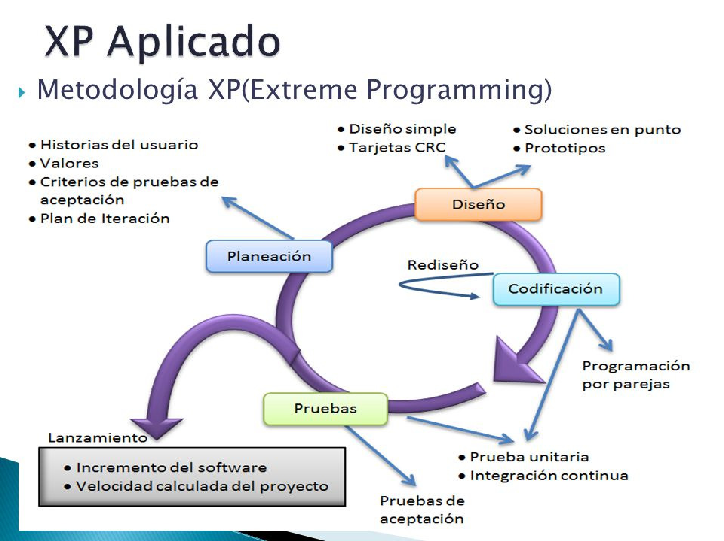
\includegraphics[width=0.7\linewidth]{image4.png}
  \caption{Ciclo de la metodología XP (Extreme Programming) aplicada al proyecto.}
  \label{fig:xp-metodologia}
\end{figure}

\textbf{Plan de Iteraciones (10 semanas)}. El proyecto se estructura en dos bloques principales de 5 semanas cada uno. El primer bloque corresponde a la fase de planeación, investigación y diseño, enfocado en mitigar riesgos y modelar la solución. El segundo bloque abarca el ciclo continuo de codificación, integración y pruebas.

\textbf{Fase I: Exploración, Diseño y Spikes Arquitectónicos}. Durante estas 5 semanas, las iteraciones se centran en el levantamiento ágil, el análisis normativo y el diseño técnico del sistema, preparando el terreno para la implementación.

\begin{itemize}
  \item \textbf{Iteración 1 (Semana 1) - Requerimientos y Fundamentos Criptográficos:} Investigación de la normativa mexicana referente al manejo de firmas digitales y comprobación de tiempo, y recolección de normativas sobre la Ley de Protección de Datos Personales. Investigación teórica de criptografía (Hash, RSA, Firma Digital) y levantamiento ágil de requerimientos funcionales y no funcionales.

  \item \textbf{Iteración 2 (Semana 2) - Análisis de Entorno y Sistemas Similares:} Investigación del Código de Procedimientos Penales Mexicanos aplicable al contexto digital. Análisis de sistemas similares en el mercado para la detección de brechas de seguridad y operativas.

  \item \textbf{Iteración 3 (Semana 3) - Análisis de Riesgos y Modelado Ágil:} Elaboración del análisis y matriz de riesgos. Traducción de los requerimientos mediante la redacción de Historias de Usuario priorizadas y diseño de los Casos de Uso del sistema.

  \item \textbf{Iteración 4 (Semana 4) - Diseño Arquitectónico y Modelo de Datos:} Diseño detallado de la arquitectura del sistema (Backend, Frontend y flujos de seguridad). Modelado de la base de datos híbrida, integrando bases de datos SQL para relaciones procesales y bases de datos Clave-Valor.

  \item \textbf{Iteración 5 (Semana 5) - Estrategia de Calidad y Cierre Documental:} Creación de la matriz de pruebas (funcionales, de integración y criptográficas). Cierre y validación documental del diseño técnico para la conclusión de la primera fase.
\end{itemize}

\textbf{Fase II: Construcción, Pruebas y Refactorización}. Una vez validado el diseño, el desarrollo entra en un ciclo estricto de codificación iterativa mediante XP, utilizando programación en pares, Desarrollo Guiado por Pruebas (TDD) y entregas continuas. El orden de las iteraciones antepone el núcleo criptográfico a la construcción de vistas: el análisis de riesgos (sección~\ref{sec:riesgos}) prescribe resolver primero los riesgos criptográficos graves y recomienda no avanzar hacia el desarrollo de vistas web hasta haber comprobado técnicamente la validez del sellado de tiempo.

\begin{itemize}
  \item \textbf{Iteración 6 (Semana 6) - Andamiaje del Workspace y Núcleo Criptográfico Base:} Configuración del workspace de Cargo con sus cinco crates y del pipeline de integración continua (formato, análisis estático, pruebas y política de dependencias). Implementación del servicio de hash SHA-256 y del cifrado autenticado AES-256-GCM con envelope encryption, proporcionando integridad y confidencialidad en reposo. Primer contacto con el sellado de tiempo mediante el Spike de consumo y parseo del token RFC 3161.

  \item \textbf{Iteración 7 (Semana 7) - PKI Interna y Firma Digital:} Implementación de la infraestructura de llave pública interna: CA raíz, emisión de certificados X.509 y lista de certificados revocados (CRL). Integración de la firma digital RSA-3072 con SHA-256 sobre los certificados emitidos. Inicio del flujo de sellado de tiempo conforme a RFC 3161.

  \item \textbf{Iteración 8 (Semana 8) - Sellado de Tiempo, Autenticación y Auditoría:} Conclusión del flujo de sellado de tiempo RFC 3161. Implementación de la autenticación (hashing de contraseñas con Argon2id y segundo factor TOTP) y de la cadena de auditoría con encadenamiento de hashes. Verificación integral de la evidencia y demostración por línea de comandos, hito de criptografía demostrada de extremo a extremo.

  \item \textbf{Iteración 9 (Semana 9) - Persistencia, Control de Acceso y Gestión Procesal:} Implementación de la persistencia híbrida PostgreSQL/Redis y del control de acceso basado en roles (RBAC) con JWT. Desarrollo de la gestión procesal y documental —módulos CRUD para expedientes, casos, contratos y documentos— integrando los servicios criptográficos ya probados. Desarrollo de una interfaz web mínima.

  \item \textbf{Iteración 10 (Semana 10) - Pruebas Finales y Cierre:} Ejecución de la matriz de pruebas diseñada en la Fase I. Pruebas de usabilidad con usuarios representativos. Corrección de errores, refactorización final de código y elaboración de los manuales técnicos y de usuario.
\end{itemize}

\section{Historias de Usuario}\label{sec:historias-usuario}

Las historias de usuario constituyen el instrumento de captura de requerimientos empleado por la metodología XP. Cada historia se redacta desde la perspectiva del actor que interactúa con el sistema, en lenguaje del dominio jurídico, estableciendo el rol, la necesidad y el beneficio esperado. Las historias se organizan en siete secciones funcionales que cubren la totalidad de los flujos del prototipo, desde la gestión de identidad hasta la operación y monitoreo del despacho. La formalización técnica de cada historia se realiza posteriormente en los casos de uso (sección~\ref{sec:casos-uso}), donde se especifican los flujos, precondiciones, postcondiciones y los mecanismos concretos de implementación.

\subsection{Autenticación, Acceso y Gestión de Identidad}\label{subsec:hu-autenticacion}

\begin{itemize}
  \item \textbf{HU-01 — Registro de despacho.} Como socio fundador, quiero registrar mi despacho en el sistema proporcionando los datos de la firma, para disponer de un espacio propio y aislado donde gestionar los expedientes y al equipo de trabajo.

  \item \textbf{HU-02 — Selección de plan de servicio.} Como socio fundador, quiero elegir un plan de servicio (Starter o Professional) al momento del registro, para que el sistema habilite las funcionalidades y los límites de usuarios correspondientes al nivel contratado.

  \item \textbf{HU-03 — Invitación de miembros al equipo.} Como socio del despacho, quiero invitar nuevos colaboradores mediante correo electrónico asignándoles un perfil (Litigante o Paralegal), para que puedan acceder al sistema con los permisos apropiados a su función.

  \item \textbf{HU-04 — Aceptación de invitación.} Como colaborador invitado, quiero aceptar la invitación recibida por correo y completar mi registro, para incorporarme al despacho con el perfil que me fue asignado.

  \item \textbf{HU-05 — Inicio de sesión con credenciales.} Como usuario del sistema, quiero autenticarme con mi correo y contraseña, para acceder a las funciones habilitadas según mi perfil.

  \item \textbf{HU-06 — Inicio de sesión con certificado digital.} Como socio del despacho, quiero iniciar sesión presentando mi certificado digital, para acceder al sistema con un nivel de seguridad superior que vincule mi identidad de forma verificable con la sesión.

  \item \textbf{HU-07 — Verificación en dos pasos.} Como cliente del despacho, quiero confirmar mi identidad con un código temporal generado en mi dispositivo después de ingresar mi contraseña, para que mi expediente esté protegido ante el robo o filtración de la contraseña.

  \item \textbf{HU-08 — Recuperación de contraseña.} Como usuario del sistema, quiero solicitar la recuperación de mi contraseña mediante correo electrónico, para restablecer el acceso a mi cuenta sin necesidad de contactar al administrador.

  \item \textbf{HU-09 — Cierre de sesión por inactividad.} Como usuario del sistema, quiero que mi sesión se cierre automáticamente tras un periodo de inactividad, para prevenir accesos no autorizados si abandono mi equipo de trabajo sin cerrar sesión.

  \item \textbf{HU-10 — Restricción de acceso por perfil.} Como socio del despacho, quiero que cada miembro del equipo solo pueda acceder a los módulos y operaciones que corresponden a su perfil, para garantizar que únicamente las personas autorizadas realicen operaciones sensibles.

  \item \textbf{HU-11 — Baja de miembros del equipo.} Como socio del despacho, quiero dar de baja a un colaborador, para revocar de inmediato su acceso al sistema y a los expedientes del despacho.
\end{itemize}

\subsection{Gestión Procesal Penal (Ciclo de Vida del Expediente)}\label{subsec:hu-procesal}

\begin{itemize}
  \item \textbf{HU-12 — Creación de expediente penal.} Como Litigante, quiero registrar un nuevo expediente ingresando el Número Único de Caso, la Carpeta Judicial, el tipo de delito y los datos generales del asunto, para que quede disponible en el sistema con estado inicial “Investigación”.

  \item \textbf{HU-13 — Registro de participantes del caso.} Como Litigante, quiero vincular a un expediente a las personas y autoridades que participan en el proceso (imputado, víctima, defensor, juez, Ministerio Público, entre otros) con sus datos identificadores y su rol dentro del proceso, para conformar el directorio de participantes del caso.

  \item \textbf{HU-14 — Avance de etapa procesal.} Como Litigante, quiero avanzar un expediente a la siguiente etapa procesal cargando el documento que lo habilita (escrito de acusación para pasar a Intermedia, auto de apertura para pasar a Juicio Oral), para que el sistema registre el cambio y habilite las funciones correspondientes a la nueva etapa.

  \item \textbf{HU-15 — Bloqueo de avance sin documento habilitante.} Como Litigante, quiero que el sistema no permita avanzar de etapa si no se ha cargado el documento procesal requerido, para evitar inconsistencias en la secuencia del expediente que comprometan su validez.

  \item \textbf{HU-16 — Historial de transiciones del expediente.} Como Litigante, quiero consultar la línea de tiempo completa de las transiciones de etapa de un expediente, con la fecha, el responsable y el documento asociado a cada cambio, para verificar que la secuencia procesal esté íntegra.

  \item \textbf{HU-17 — Actualización de datos del expediente.} Como Litigante, quiero actualizar los datos generales de un expediente (delitos, identificadores complementarios, información general), para mantener la información vigente sin alterar el historial de transiciones.

  \item \textbf{HU-18 — Vista de expedientes asignados.} Como Paralegal, quiero visualizar únicamente los expedientes que me han sido asignados, para concentrarme en los casos relevantes a mi trabajo sin exposición a información de otros asuntos.
\end{itemize}

\subsection{Calendario Jurídico, Plazos y Alertas}\label{subsec:hu-calendario}

\begin{itemize}
  \item \textbf{HU-19 — Programación de audiencia.} Como Litigante, quiero agendar una audiencia seleccionando su tipo (inicial, intermedia, juicio oral, individualización de sanciones), fecha, hora, participantes y modalidad, para que quede vinculada al expediente correspondiente.

  \item \textbf{HU-20 — Activación automática de plazos tras audiencia.} Como Litigante, quiero que al registrar el resultado de una audiencia (por ejemplo, vinculación a proceso), el sistema calcule y active automáticamente los plazos derivados (como el de investigación complementaria), para no depender del cálculo manual de los términos.

  \item \textbf{HU-21 — Cómputo de plazos con días inhábiles.} Como Litigante, quiero que el sistema calcule las fechas de vencimiento descontando correctamente sábados, domingos y días inhábiles del calendario judicial de la entidad federativa, para obtener fechas precisas conforme a las reglas de cómputo del CNPP.

  \item \textbf{HU-22 — Configuración del calendario judicial.} Como socio del despacho, quiero configurar los días inhábiles por entidad federativa y fuero, para que los cómputos de plazos reflejen los periodos de receso de cada jurisdicción donde litiga el despacho.

  \item \textbf{HU-23 — Alertas de vencimiento próximo.} Como Litigante, quiero recibir notificaciones automáticas por correo y en el sistema cuando un plazo esté próximo a vencer, para tomar acciones oportunas y evitar consecuencias procesales irreversibles.

  \item \textbf{HU-24 — Calendario unificado del despacho.} Como Litigante, quiero visualizar en un calendario interactivo todas las audiencias programadas y los plazos límite de mis casos, con colores diferenciados por tipo de evento y acceso directo al expediente, para gestionar mi agenda procesal desde una sola vista.
\end{itemize}

\subsection{Gestión Documental y Cadena de Custodia}\label{subsec:hu-documental}

\begin{itemize}
  \item \textbf{HU-25 — Carga de documento al expediente.} Como Litigante, quiero cargar un documento procesal asociándolo a un expediente, para que quede almacenado de forma protegida y disponible para consulta por las personas autorizadas.

  \item \textbf{HU-26 — Clasificación de documentos.} Como Litigante, quiero asignar tipo documental, clasificación y etiquetas a cada documento cargado, para facilitar su organización, búsqueda y recuperación dentro del expediente.

  \item \textbf{HU-27 — Consulta de documentos según asignación.} Como Paralegal, quiero consultar y descargar los documentos de los expedientes que tengo asignados, para apoyar la gestión del caso sin acceder a información de asuntos no relacionados.

  \item \textbf{HU-28 — Registro automático de movimientos sobre documentos.} Como Litigante, quiero que cada operación sobre un documento o evidencia (carga, consulta, descarga, movimiento) quede registrada automáticamente con la fecha, la persona responsable y el tipo de operación, para contar con un historial completo que respalde la cadena de custodia del expediente.

  \item \textbf{HU-29 — Protección del historial de movimientos.} Como Litigante, quiero que ningún usuario, incluido el socio del despacho, pueda modificar ni eliminar los registros del historial de movimientos de documentos, para garantizar que la trazabilidad sea confiable ante cualquier requerimiento judicial.
\end{itemize}

\subsection{Servicios de Protección de la Información}\label{subsec:hu-proteccion}

\begin{itemize}
  \item \textbf{HU-30 — Huella digital del documento al momento de carga.} Como Litigante, quiero que al cargar un documento al sistema, se genere automáticamente una huella digital única del archivo, para contar con una referencia que permita comprobar en el futuro si el documento fue alterado.

  \item \textbf{HU-31 — Alerta de alteración en consulta posterior.} Como Litigante, quiero que cada vez que consulte un documento, el sistema verifique automáticamente que no haya sido modificado desde su carga y me alerte de inmediato si detecta alguna discrepancia, para tener certeza de la inalterabilidad de mis expedientes.

  \item \textbf{HU-32 — Protección del contenido almacenado.} Como Litigante, quiero que los documentos de mis expedientes se almacenen protegidos de forma que solo las partes autorizadas puedan acceder a su contenido, para que una intrusión al sistema no exponga la información de mis clientes.

  \item \textbf{HU-33 — Detección de manipulación en el almacenamiento.} Como Litigante, quiero que si alguien manipula directamente los archivos almacenados en el servidor, el sistema lo detecte y rechace la entrega del documento afectado notificándome la anomalía, para saber que cualquier intento de alteración será evidenciado.
\end{itemize}

\subsection{Firma de Contratos y Constancia de Fecha}\label{subsec:hu-firma}

\begin{itemize}
  \item \textbf{HU-34 — Firma de contrato con identidad verificable.} Como Litigante, quiero firmar un contrato de manera que mi identidad quede vinculada de forma verificable con el contenido del documento, para que ninguna de las partes pueda negar posteriormente haber suscrito el acuerdo.

  \item \textbf{HU-35 — Constancia de fecha y hora de la firma.} Como Litigante, quiero que al firmar un contrato, el sistema obtenga automáticamente una constancia emitida por una autoridad certificadora que acredite la fecha y hora exacta de la firma, para que el documento tenga valor probatorio conforme a la normatividad mexicana.

  \item \textbf{HU-36 — Verificación de firma y constancia de un contrato.} Como usuario con acceso al contrato, quiero poder ejecutar una verificación que me indique si la firma es válida, si el certificado del firmante está vigente y si la constancia de fecha es auténtica, para evaluar la confiabilidad del documento sin depender de un tercero.

  \item \textbf{HU-37 — Detección de alteración en contrato firmado.} Como usuario con acceso al contrato, quiero que si el documento fue modificado después de firmado, la verificación me indique claramente que la firma ya no es válida y me explique la causa, para disponer de evidencia de que el contrato fue alterado.
\end{itemize}

\subsection{Operación y Monitoreo}\label{subsec:hu-operacion}

\begin{itemize}
  \item \textbf{HU-38 — Tablero de control del despacho.} Como socio del despacho, quiero consultar un tablero con indicadores clave (casos activos, plazos por vencer próximamente, contratos pendientes de firma, carga de trabajo por abogado), para tener visibilidad del estado general de la operación.

  \item \textbf{HU-39 — Generación de informes.} Como socio del despacho, quiero generar informes filtrados por periodo, abogado responsable o estado de los casos, exportables en formato descargable, para analizar el desempeño y las métricas operativas de la firma.

  \item \textbf{HU-40 — Registro general de actividad.} Como socio del despacho, quiero consultar un registro completo e inalterable de todas las acciones realizadas en el sistema (quién realizó la acción, qué hizo, sobre qué recurso y cuándo), para disponer de trazabilidad ante auditorías internas o requerimientos judiciales.
\end{itemize}


\section{Casos de Uso}\label{sec:casos-uso}

Los casos de uso formalizan las historias de usuario definidas en la \cref{sec:historias-usuario}, especificando los flujos de interacción entre los actores y el sistema, las condiciones que deben cumplirse antes y después de cada operación, y los escenarios alternos que el prototipo debe manejar. Cada caso de uso agrupa una o más historias de usuario en un flujo funcional cohesivo e incluye la trazabilidad hacia los requerimientos funcionales y no funcionales que lo respaldan. La especificación técnica de los mecanismos criptográficos (algoritmos, estándares y protocolos) se detalla en los requerimientos de la \cref{sec:requerimientos}; los casos de uso se limitan a describir el comportamiento observable del sistema desde la perspectiva del actor.

\subsection{Autenticación, Acceso y Gestión de Identidad}\label{sec:cu-autenticacion}

\subsubsection{CU-01 --- Registro de despacho y selección de plan}

\begin{table}[H]
  \centering
  \caption{Caso de uso CU-01: Registro de despacho y selección de plan.}
  \label{tab:cu-01}
  \begin{tabularx}{\linewidth}{@{}>{\bfseries}l X@{}}
    \toprule
    ID & \textbf{CU-01} \\
    \midrule
    Nombre & Registro de despacho y selección de plan \\
    Actor principal & Socio fundador \\
    Actores secundarios & Sistema de correo transaccional \\
    Precondiciones & El usuario no posee una cuenta activa en el sistema. \\
    Flujo principal & 1. El usuario accede al formulario de registro. 2. Ingresa los datos del despacho (nombre de la firma, domicilio fiscal, datos de contacto). 3. Selecciona un plan de servicio (Starter o Professional). 4. Establece sus credenciales de acceso (correo y contraseña). 5. El sistema valida los datos ingresados y aprovisiona el espacio de trabajo del despacho con el plan seleccionado. 6. El sistema envía un correo de confirmación al socio fundador. 7. El socio fundador confirma su correo electrónico mediante el enlace recibido. 8. El sistema activa la cuenta y redirige al tablero de control del despacho. \\
    Flujos alternos & 4a. La contraseña no cumple las políticas de complejidad → el sistema indica los requisitos faltantes. 5a. El correo electrónico ya está registrado → el sistema informa que la cuenta existe y ofrece la opción de recuperación. 7a. El enlace de confirmación ha expirado → el sistema permite reenviar el correo de confirmación. \\
    Postcondiciones & El despacho queda registrado con su espacio de datos inicializado, el plan activo y el socio fundador autenticado con rol Owner. Las credenciales se almacenan mediante funciones de hashing resistentes. \\
    Derivado de & HU-01, HU-02 \\
    RF relacionados & RF-01, RF-02 \\
    RNF relacionados & RNF-01, RNF-02 \\
    \bottomrule
  \end{tabularx}
\end{table}

\begin{figure}[H]
  \centering
  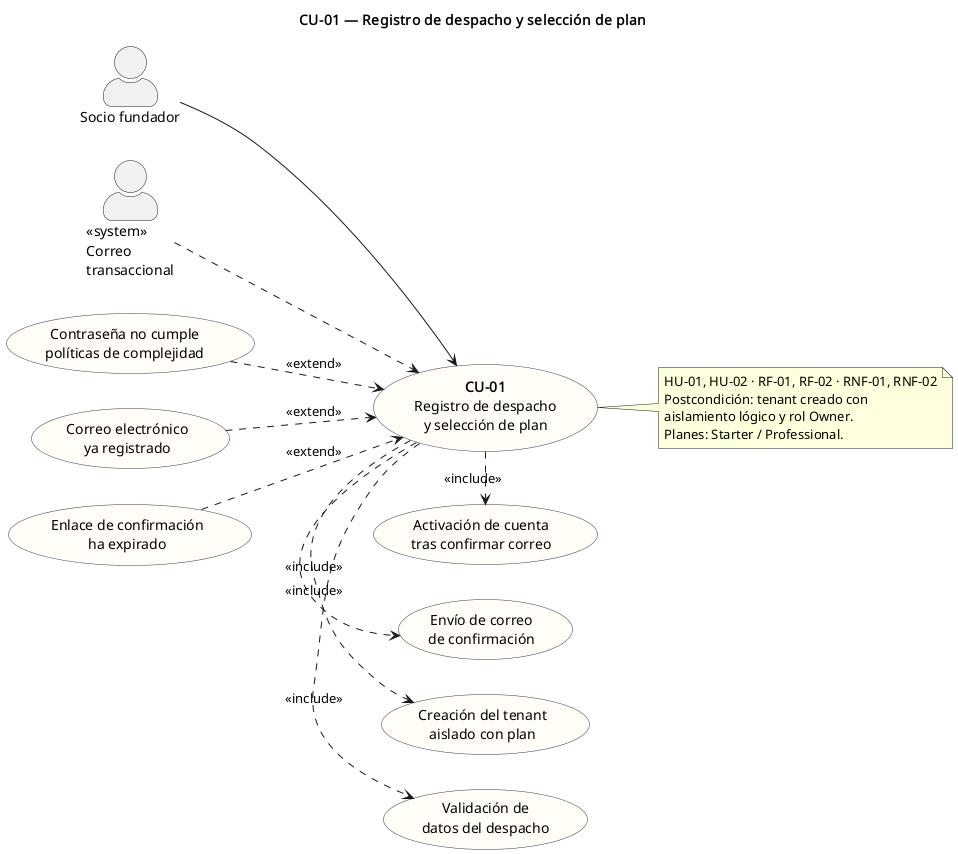
\includegraphics[width=0.9\linewidth]{image5.png}
  \caption{Diagrama CU-01. Registro de despacho y selección de plan.}
  \label{fig:cu-01}
\end{figure}

\subsubsection{CU-02 --- Gestión del ciclo de vida de miembros del equipo}

\begin{table}[H]
  \centering
  \caption{Caso de uso CU-02: Gestión del ciclo de vida de miembros del equipo.}
  \label{tab:cu-02}
  \begin{tabularx}{\linewidth}{@{}>{\bfseries}l X@{}}
    \toprule
    ID & \textbf{CU-02} \\
    \midrule
    Nombre & Gestión del ciclo de vida de miembros del equipo \\
    Actor principal & Owner \\
    Actores secundarios & Colaborador invitado, sistema de correo transaccional \\
    Precondiciones & El Owner tiene sesión activa. \\
    Flujo principal (alta) & 1. El Owner accede al módulo de gestión de equipo. 2. Ingresa el correo electrónico del nuevo miembro y selecciona el perfil a asignar (Litigante o Paralegal). 3. El sistema verifica que el despacho no ha alcanzado el límite de usuarios del plan contratado. 4. El sistema genera un enlace de invitación con vigencia limitada y lo envía por correo. 5. El colaborador invitado accede al enlace, completa su registro con sus datos personales y establece su contraseña. 6. El sistema valida los datos, crea la cuenta asociada al despacho con el perfil indicado y registra la operación en la bitácora. 7. El nuevo miembro accede al sistema con las funciones habilitadas según su perfil. \\
    Flujo principal (baja) & 1. El Owner accede al módulo de gestión de equipo. 2. Selecciona al miembro que desea dar de baja. 3. El sistema solicita confirmación de la acción. 4. El Owner confirma la baja. 5. El sistema revoca de inmediato el acceso del colaborador, invalida sus sesiones activas y registra la operación en la bitácora. 6. Los expedientes y documentos asociados al colaborador permanecen en el sistema sin modificación; únicamente se revoca el acceso. \\
    Flujos alternos & 2a. (Alta) El correo ya pertenece a un miembro activo del despacho → el sistema rechaza la invitación e informa el motivo. 3a. (Alta) El despacho ha alcanzado el límite de usuarios → el sistema bloquea la invitación e indica la necesidad de actualizar el plan. 5a. (Alta) El enlace de invitación ha expirado → el sistema muestra un mensaje informativo; el Owner debe reenviar la invitación. 2b. (Baja) El Owner intenta darse de baja a sí mismo → el sistema rechaza la operación, ya que el despacho requiere al menos un Owner activo. \\
    Postcondiciones & (Alta) El colaborador queda registrado en el despacho con el perfil asignado. (Baja) El acceso del colaborador queda revocado de inmediato. En ambos casos, la operación se registra en la bitácora de actividad. \\
    Derivado de & HU-03, HU-04, HU-11 \\
    RF relacionados & RF-03 \\
    RNF relacionados & RNF-01, RNF-02 \\
    \bottomrule
  \end{tabularx}
\end{table}

\begin{figure}[H]
  \centering
  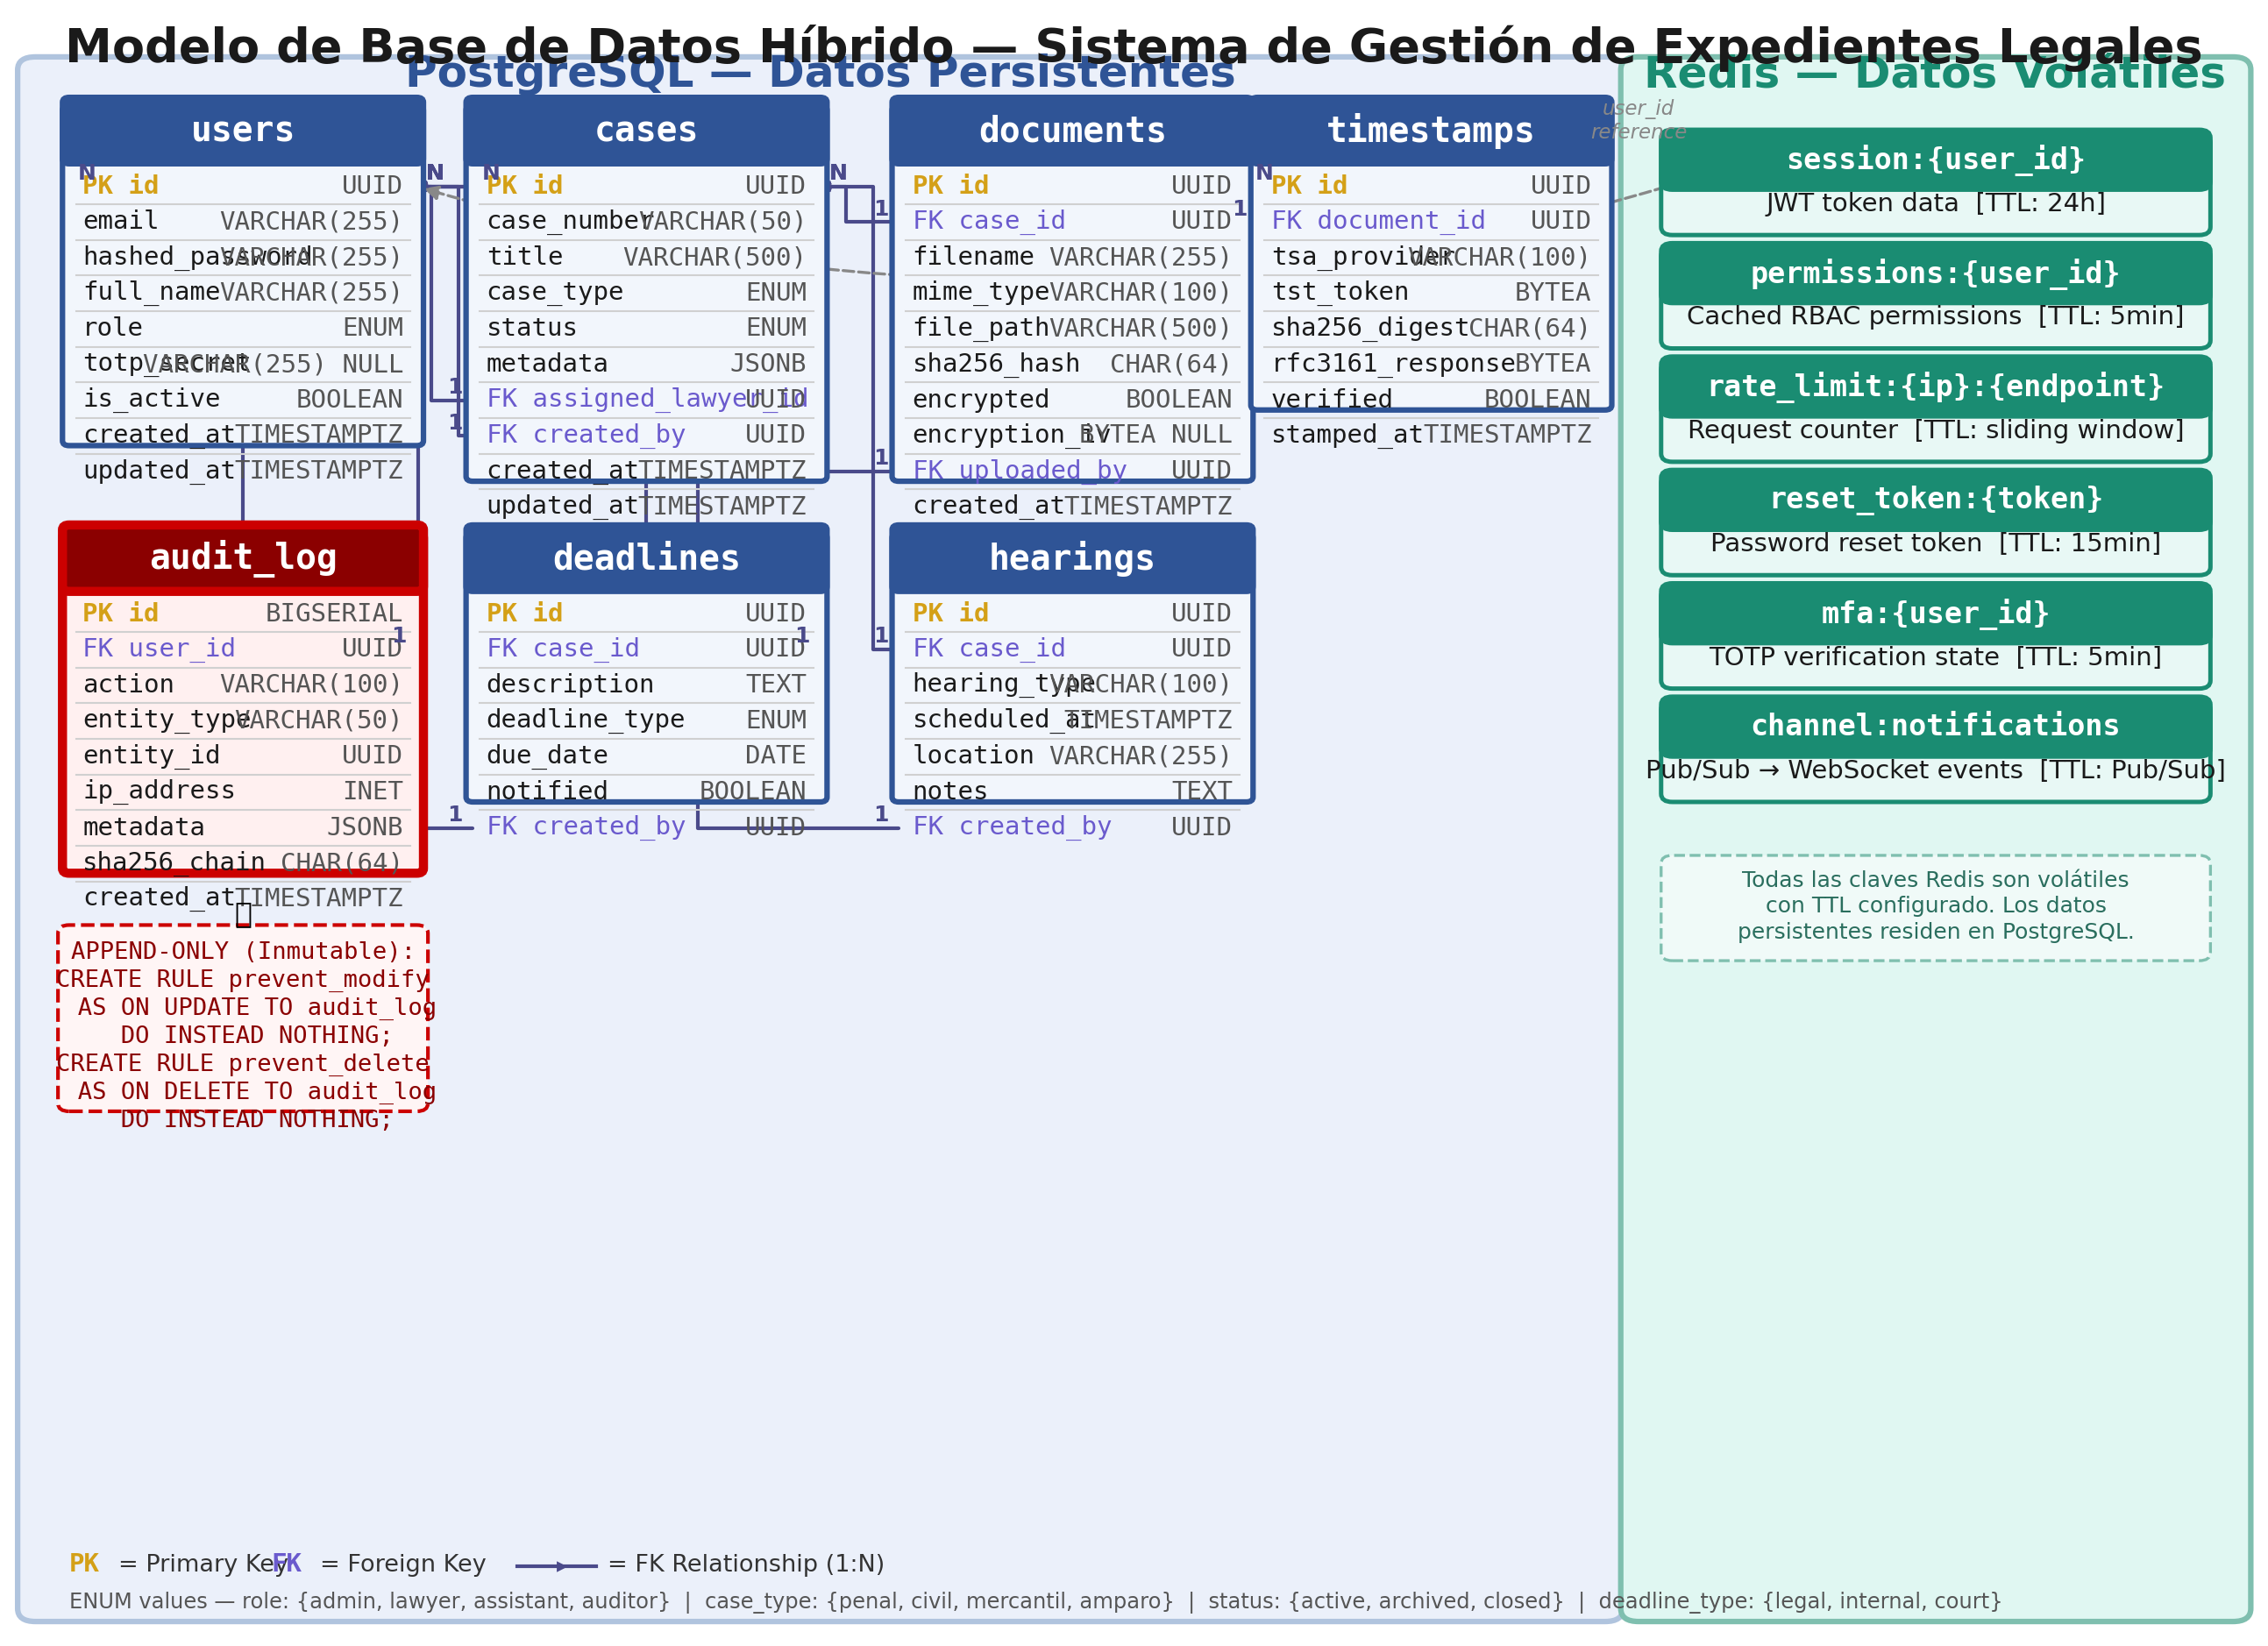
\includegraphics[width=0.9\linewidth]{image6.png}
  \caption{Diagrama CU-02. Gestión del ciclo de vida de miembros del equipo.}
  \label{fig:cu-02}
\end{figure}

\subsubsection{CU-03 --- Inicio de sesión y gestión de sesiones}

\begin{table}[H]
  \centering
  \caption{Caso de uso CU-03: Inicio de sesión y gestión de sesiones.}
  \label{tab:cu-03}
  \begin{tabularx}{\linewidth}{@{}>{\bfseries}l X@{}}
    \toprule
    ID & \textbf{CU-03} \\
    \midrule
    Nombre & Inicio de sesión y gestión de sesiones \\
    Actor principal & Usuario del sistema (Owner, Litigante, Paralegal, Cliente) \\
    Actores secundarios & --- \\
    Precondiciones & El usuario posee una cuenta activa en el sistema. \\
    Flujo principal & 1. El usuario accede a la pantalla de inicio de sesión. 2. Ingresa su correo electrónico y contraseña. 3. El sistema verifica las credenciales contra el hash almacenado. 4. Si el usuario tiene habilitada la verificación en dos pasos, el sistema solicita el código temporal generado en su dispositivo. 5. El usuario ingresa el código y el sistema lo valida. 6. El sistema crea una sesión autenticada, registra el inicio de sesión en la bitácora y redirige al usuario al módulo correspondiente a su perfil. \\
    Flujos alternos & 3a. Las credenciales son incorrectas → el sistema informa el error sin revelar cuál campo es inválido. 3b. El usuario es Owner y elige autenticarse con certificado digital → el sistema genera un desafío criptográfico; el usuario firma con su clave privada; el sistema verifica la firma contra el certificado registrado. 1a. El usuario selecciona la opción de recuperación de contraseña → el sistema solicita el correo electrónico asociado a la cuenta → envía un enlace de restablecimiento con vigencia limitada → el usuario accede al enlace y establece una nueva contraseña → el sistema la almacena mediante funciones de hashing resistentes, invalida las sesiones activas previas y confirma el restablecimiento. 5a. El código temporal es inválido o ha expirado → el sistema rechaza el acceso y permite reintentar. 6a. La sesión permanece inactiva por el tiempo configurado → el sistema la invalida y requiere nueva autenticación, preservando los datos no guardados. \\
    Postcondiciones & El usuario queda autenticado con una sesión activa. El inicio de sesión, incluyendo método de autenticación utilizado y dirección IP, se registra en la bitácora. \\
    Derivado de & HU-05, HU-06, HU-07, HU-08, HU-09 \\
    RF relacionados & RF-01, RF-02 \\
    RNF relacionados & RNF-02, RNF-05 \\
    \bottomrule
  \end{tabularx}
\end{table}

\begin{figure}[H]
  \centering
  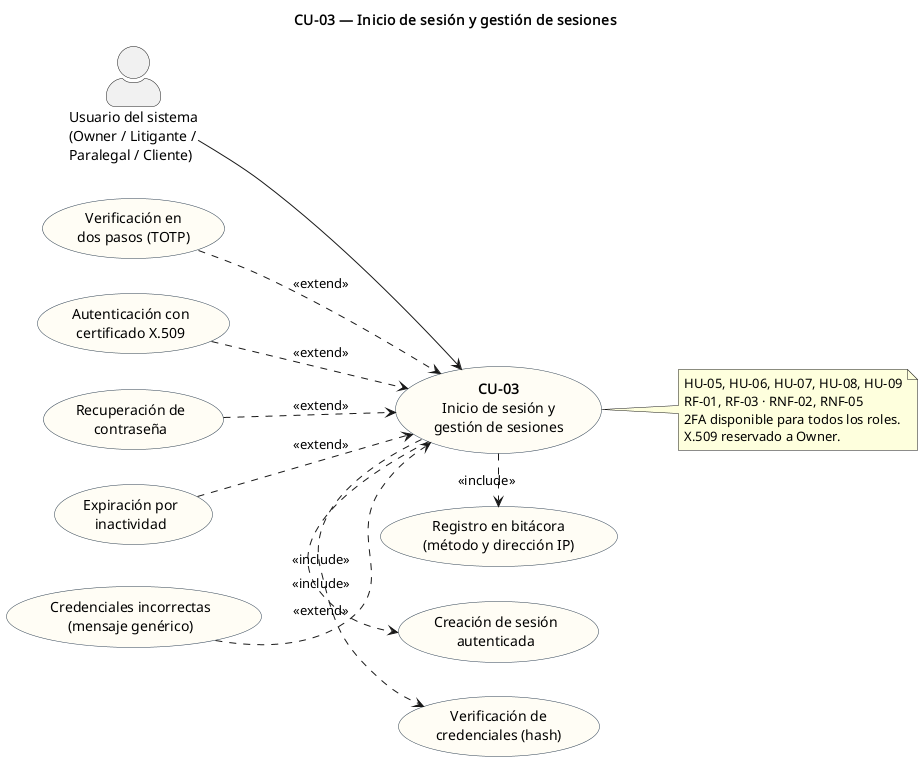
\includegraphics[width=0.9\linewidth]{image7.png}
  \caption{Diagrama CU-03. Inicio de sesión y gestión de sesiones.}
  \label{fig:cu-03}
\end{figure}

\subsubsection{CU-04 --- Control de acceso por perfil}

\begin{table}[H]
  \centering
  \caption{Caso de uso CU-04: Control de acceso por perfil.}
  \label{tab:cu-04}
  \begin{tabularx}{\linewidth}{@{}>{\bfseries}l X@{}}
    \toprule
    ID & \textbf{CU-04} \\
    \midrule
    Nombre & Control de acceso por perfil \\
    Actor principal & Usuario autenticado (cualquier rol) \\
    Actores secundarios & --- \\
    Precondiciones & El usuario tiene sesión activa. \\
    Flujo principal & 1. El usuario solicita acceso a un módulo o recurso del sistema. 2. El sistema evalúa el perfil del usuario contra la matriz de permisos del módulo solicitado. 3. Si el perfil tiene permiso, el sistema concede el acceso y presenta la interfaz correspondiente. \\
    Flujos alternos & 3a. El perfil no tiene permiso sobre el módulo solicitado → el sistema deniega el acceso con un mensaje explicativo y registra el intento en la bitácora. 3b. El usuario intenta acceder a un recurso fuera de su ámbito de autorización (por ejemplo, manipulando identificadores de expedientes no asignados) → el sistema devuelve un error de autorización sin revelar la existencia del recurso. \\
    Postcondiciones & El acceso queda concedido o denegado. Cada intento de acceso, exitoso o fallido, se registra en la bitácora. \\
    Derivado de & HU-10 \\
    RF relacionados & RF-02 \\
    RNF relacionados & RNF-01, RNF-05 \\
    \bottomrule
  \end{tabularx}
\end{table}

\begin{figure}[H]
  \centering
  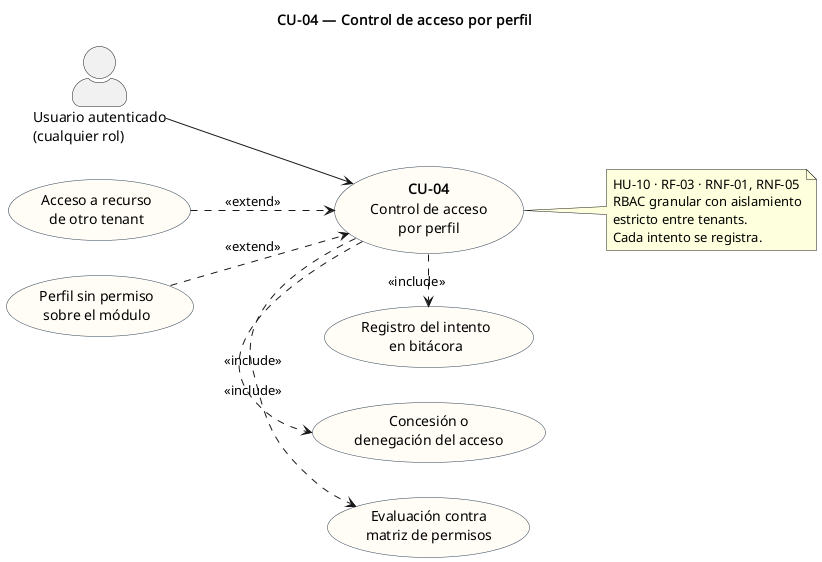
\includegraphics[width=0.9\linewidth]{image8.png}
  \caption{Diagrama CU-04. Control de acceso por perfil.}
  \label{fig:cu-04}
\end{figure}

\subsection{Gestión Procesal Penal (Ciclo de Vida del Expediente)}\label{sec:cu-gestion-procesal}

\subsubsection{CU-05 --- Registro y administración de expediente penal}

\begin{table}[H]
  \centering
  \caption{Caso de uso CU-05: Registro y administración de expediente penal.}
  \label{tab:cu-05}
  \begin{tabularx}{\linewidth}{@{}>{\bfseries}l X@{}}
    \toprule
    ID & \textbf{CU-05} \\
    \midrule
    Nombre & Registro y administración de expediente penal \\
    Actor principal & Litigante \\
    Actores secundarios & Paralegal (consulta) \\
    Precondiciones & El Litigante tiene sesión activa y pertenece al despacho. \\
    Flujo principal & 1. El Litigante accede al módulo de gestión procesal y selecciona la opción de nuevo expediente. 2. Ingresa los identificadores oficiales: Número Único de Caso (NUC) y Carpeta Judicial. 3. Registra el tipo de delito, los datos generales del asunto y los metadatos asociados. 4. El sistema valida que los campos obligatorios estén completos y que los identificadores no estén duplicados dentro del despacho. 5. El sistema persiste el expediente con estado inicial “Investigación”, genera la marca de tiempo de creación y registra la operación en la bitácora. \\
    Flujos alternos & 4a. Faltan campos obligatorios (NUC o Carpeta Judicial) → el sistema rechaza el registro e indica los campos faltantes. 4b. El NUC ya existe en el despacho → el sistema informa la duplicidad. \\
    Postcondiciones & El expediente queda registrado con estado “Investigación”, disponible para los usuarios autorizados del despacho. \\
    Derivado de & HU-12, HU-17, HU-18 \\
    RF relacionados & RF-04 \\
    RNF relacionados & RNF-04, RNF-10 \\
    \bottomrule
  \end{tabularx}
\end{table}

\begin{figure}[H]
  \centering
  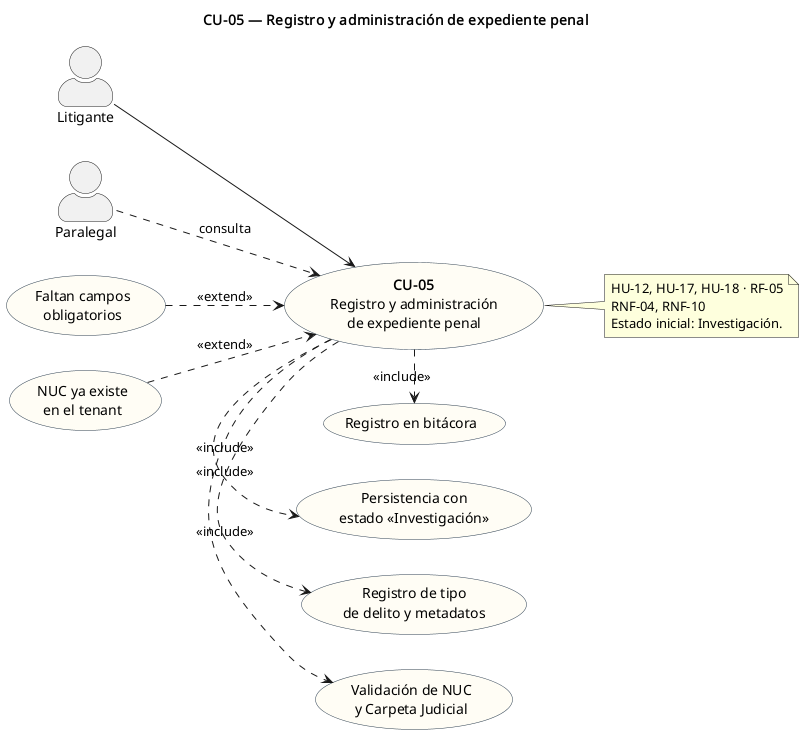
\includegraphics[width=0.9\linewidth]{image9.png}
  \caption{Diagrama CU-05. Registro y administración de expediente penal.}
  \label{fig:cu-05}
\end{figure}

\subsubsection{CU-06 --- Gestión del directorio de participantes}

\begin{table}[H]
  \centering
  \caption{Caso de uso CU-06: Gestión del directorio de participantes.}
  \label{tab:cu-06}
  \begin{tabularx}{\linewidth}{@{}>{\bfseries}l X@{}}
    \toprule
    ID & \textbf{CU-06} \\
    \midrule
    Nombre & Gestión del directorio de participantes \\
    Actor principal & Litigante \\
    Actores secundarios & --- \\
    Precondiciones & Existe un expediente activo al cual vincular participantes. \\
    Flujo principal & 1. El Litigante accede al expediente y selecciona el módulo de directorio de participantes. 2. Selecciona el tipo de sujeto procesal (imputado, víctima, defensor, juez de control, Ministerio Público, entre otros). 3. Ingresa los datos identificadores del participante según su tipo (nombre, CURP, cédula profesional, órgano jurisdiccional, según aplique). 4. El sistema valida los datos requeridos según el tipo de sujeto procesal y registra al participante vinculado al expediente. \\
    Flujos alternos & 3a. Para un juez de control, no se proporciona el órgano jurisdiccional ni la FIREL → el sistema rechaza el registro e indica los campos faltantes. 4a. El participante ya existe en el directorio del caso con el mismo rol → el sistema informa la duplicidad. \\
    Postcondiciones & El participante queda vinculado al expediente con su rol procesal. Un mismo individuo puede tener roles distintos en expedientes diferentes. \\
    Derivado de & HU-13 \\
    RF relacionados & RF-06 \\
    RNF relacionados & RNF-10 \\
    \bottomrule
  \end{tabularx}
\end{table}

\begin{figure}[H]
  \centering
  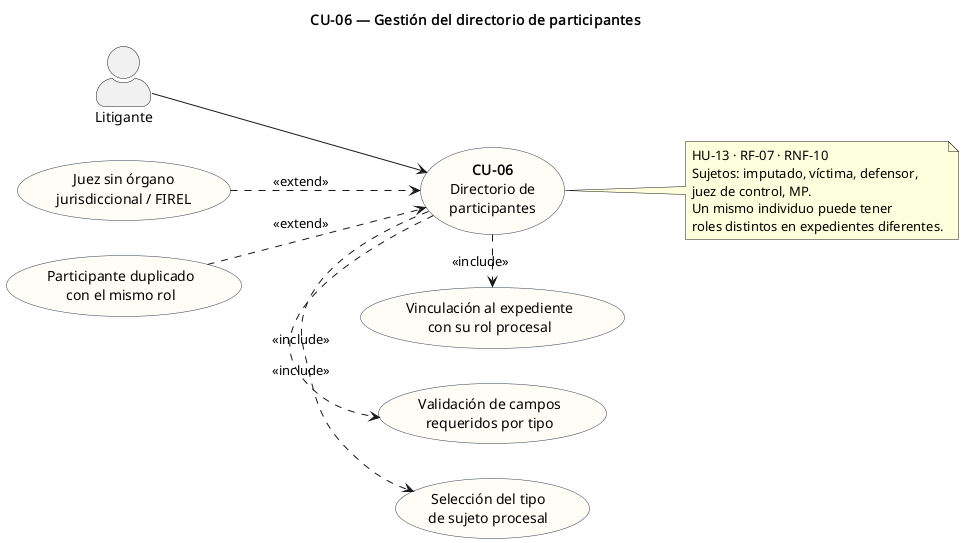
\includegraphics[width=0.9\linewidth]{image10.png}
  \caption{Diagrama CU-06. Gestión del directorio de participantes.}
  \label{fig:cu-06}
\end{figure}

\subsubsection{CU-07 --- Transición de etapa procesal}

\begin{table}[H]
  \centering
  \caption{Caso de uso CU-07: Transición de etapa procesal.}
  \label{tab:cu-07}
  \begin{tabularx}{\linewidth}{@{}>{\bfseries}l X@{}}
    \toprule
    ID & \textbf{CU-07} \\
    \midrule
    Nombre & Transición de etapa procesal \\
    Actor principal & Litigante \\
    Actores secundarios & --- \\
    Precondiciones & El expediente se encuentra en una etapa procesal que admite transición (Investigación, Intermedia o Juicio Oral). \\
    Flujo principal & 1. El Litigante accede al expediente y solicita avanzar a la siguiente etapa procesal. 2. El sistema solicita la carga del documento habilitante correspondiente (escrito de acusación para Investigación → Intermedia; auto de apertura para Intermedia → Juicio Oral). 3. El Litigante carga el documento procesal. 4. El sistema almacena el documento con las protecciones de integridad y confidencialidad correspondientes. 5. El sistema registra la transición de forma inmutable: marca de tiempo, usuario responsable y documento asociado. 6. El sistema habilita los módulos correspondientes a la nueva etapa. \\
    Flujos alternos & 2a. El Litigante intenta avanzar de etapa sin cargar el documento habilitante → el sistema rechaza la transición e indica el documento requerido. 3a. El documento cargado no corresponde al formato admitido → el sistema rechaza la carga. \\
    Postcondiciones & El expediente se encuentra en la nueva etapa procesal. La transición queda registrada de forma inmutable en el historial del expediente y no puede revertirse. \\
    Derivado de & HU-14, HU-15, HU-16 \\
    RF relacionados & RF-05 \\
    RNF relacionados & RNF-04, RNF-10 \\
    \bottomrule
  \end{tabularx}
\end{table}

\begin{figure}[H]
  \centering
  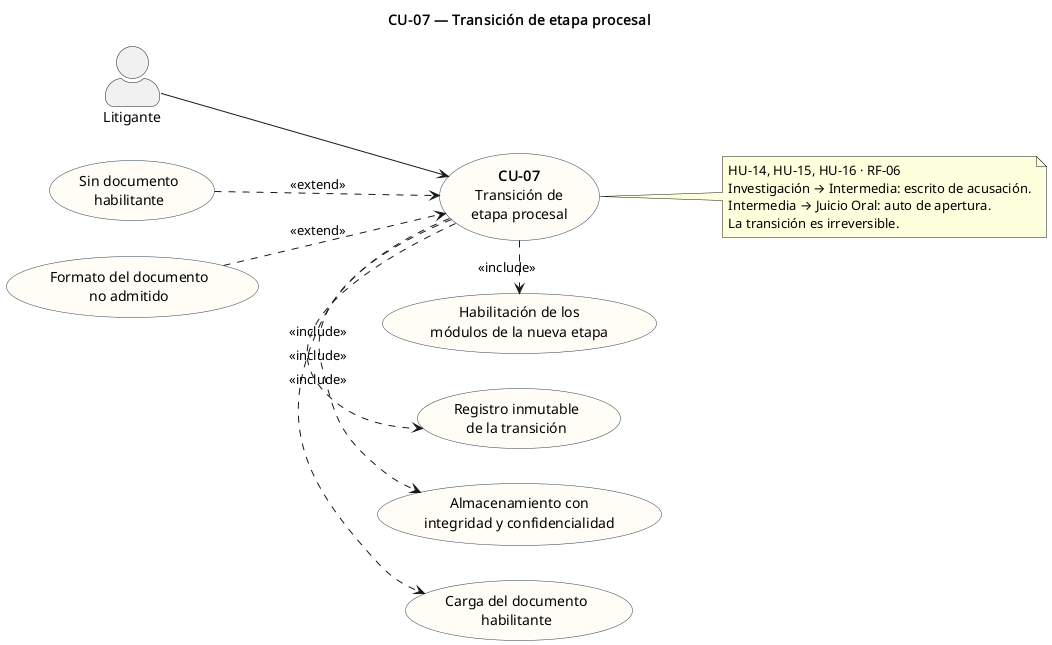
\includegraphics[width=0.9\linewidth]{image11.png}
  \caption{Diagrama CU-07. Transición de etapa procesal.}
  \label{fig:cu-07}
\end{figure}

\subsection{Calendario Jurídico, Plazos y Alertas}\label{sec:cu-calendario}

\subsubsection{CU-08 --- Programación de audiencia y activación de plazos}

\begin{table}[H]
  \centering
  \caption{Caso de uso CU-08: Programación de audiencia y activación de plazos.}
  \label{tab:cu-08}
  \begin{tabularx}{\linewidth}{@{}>{\bfseries}l X@{}}
    \toprule
    ID & \textbf{CU-08} \\
    \midrule
    Nombre & Programación de audiencia y activación de plazos \\
    Actor principal & Litigante \\
    Actores secundarios & Sistema de cómputo de plazos \\
    Precondiciones & Existe un expediente activo con una etapa procesal que admite la audiencia a programar. \\
    Flujo principal & 1. El Litigante accede al expediente y selecciona la opción de programar audiencia. 2. Selecciona el tipo de audiencia del catálogo tipificado conforme al CNPP (inicial, intermedia, juicio oral, individualización de sanciones). 3. Ingresa fecha, hora, participantes y modalidad (presencial o videoconferencia). 4. El sistema valida la coherencia procesal (el tipo de audiencia corresponde a la etapa vigente del expediente). 5. El sistema registra la audiencia vinculada al expediente. 6. Al registrar el resultado de la audiencia (por ejemplo, vinculación a proceso), el sistema activa automáticamente los plazos derivados, calculando las fechas de vencimiento conforme a las reglas del artículo 94 del CNPP (véase §2.2.5) y al calendario de días inhábiles configurado. \\
    Flujos alternos & 4a. El tipo de audiencia no corresponde a la etapa procesal vigente → el sistema rechaza la programación. 6a. El resultado de la audiencia no genera plazos derivados → el sistema registra el resultado sin activar cómputos adicionales. \\
    Postcondiciones & La audiencia queda registrada y visible en el calendario del despacho. Los plazos derivados, si los hay, quedan activos con sus fechas de vencimiento calculadas y las alertas preventivas programadas. \\
    Derivado de & HU-19, HU-20, HU-21 \\
    RF relacionados & RF-07, RF-08 \\
    RNF relacionados & RNF-10 \\
    \bottomrule
  \end{tabularx}
\end{table}

\begin{figure}[H]
  \centering
  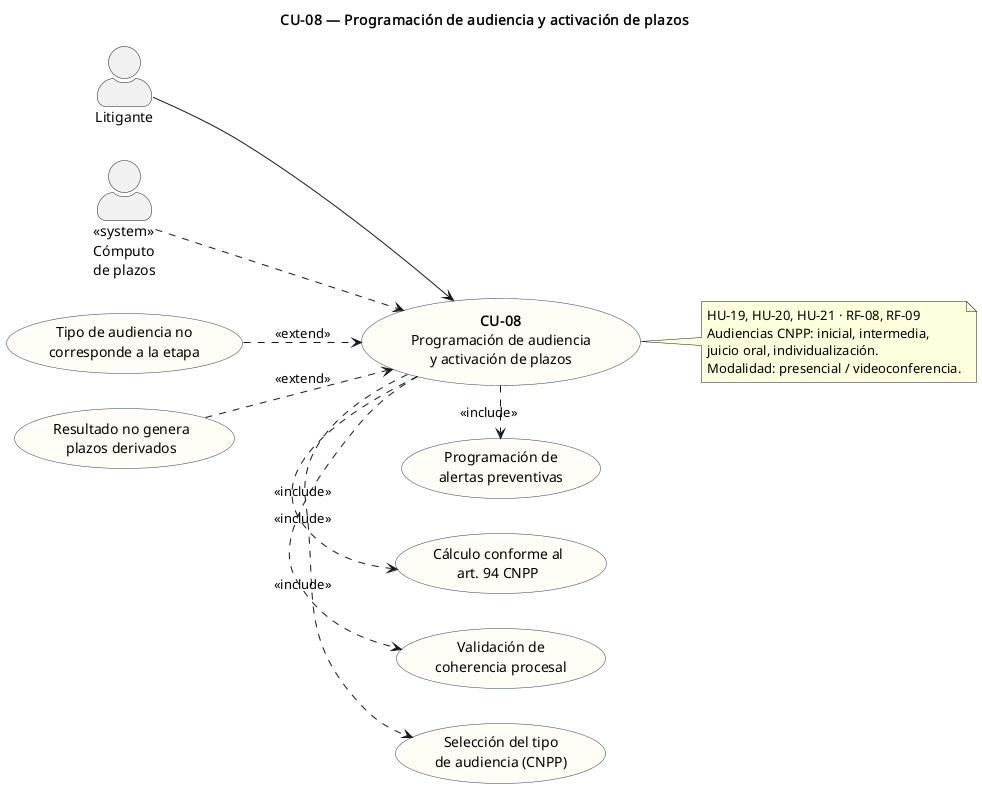
\includegraphics[width=0.9\linewidth]{image12.png}
  \caption{Diagrama CU-08. Programación de audiencia y activación de plazos.}
  \label{fig:cu-08}
\end{figure}

\subsubsection{CU-09 --- Configuración del calendario judicial}

\begin{table}[H]
  \centering
  \caption{Caso de uso CU-09: Configuración del calendario judicial.}
  \label{tab:cu-09}
  \begin{tabularx}{\linewidth}{@{}>{\bfseries}l X@{}}
    \toprule
    ID & \textbf{CU-09} \\
    \midrule
    Nombre & Configuración del calendario judicial \\
    Actor principal & Owner \\
    Actores secundarios & --- \\
    Precondiciones & El Owner tiene sesión activa. \\
    Flujo principal & 1. El Owner accede al módulo de configuración del despacho. 2. Selecciona la entidad federativa y el fuero para los cuales configurará los días inhábiles. 3. Registra los periodos de receso judicial, días feriados y días inhábiles específicos de la jurisdicción. 4. El sistema almacena la configuración y recalcula los plazos activos que dependan de ese calendario. \\
    Flujos alternos & 3a. Se registra un día inhábil que afecta un plazo con vencimiento inminente (menos de 48 horas) → el sistema recalcula la fecha y emite una alerta al Litigante responsable. \\
    Postcondiciones & El calendario judicial del despacho queda actualizado. Todos los cómputos de plazos futuros utilizan la configuración vigente. \\
    Derivado de & HU-22 \\
    RF relacionados & RF-08 \\
    RNF relacionados & RNF-10 \\
    \bottomrule
  \end{tabularx}
\end{table}

\begin{figure}[H]
  \centering
  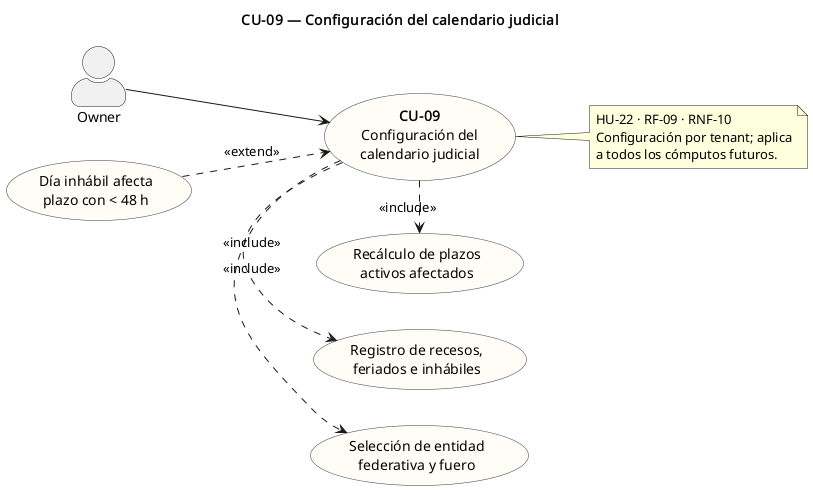
\includegraphics[width=0.9\linewidth]{image13.png}
  \caption{Diagrama CU-09. Configuración del calendario judicial.}
  \label{fig:cu-09}
\end{figure}

\subsubsection{CU-10 --- Monitoreo de plazos y emisión de alertas}

\begin{table}[H]
  \centering
  \caption{Caso de uso CU-10: Monitoreo de plazos y emisión de alertas.}
  \label{tab:cu-10}
  \begin{tabularx}{\linewidth}{@{}>{\bfseries}l X@{}}
    \toprule
    ID & \textbf{CU-10} \\
    \midrule
    Nombre & Monitoreo de plazos y emisión de alertas \\
    Actor principal & Sistema (proceso automático) \\
    Actores secundarios & Litigante (receptor de alertas), sistema de correo transaccional \\
    Precondiciones & Existen plazos activos en el sistema. \\
    Flujo principal & 1. El sistema ejecuta periódicamente la verificación de plazos activos. 2. Para cada plazo próximo a vencer (dentro del umbral configurado: 48 h y 24 h por defecto), el sistema genera una notificación. 3. La notificación se envía al Litigante responsable por correo electrónico y se muestra como alerta en el tablero de control. 4. El envío de la notificación se registra en la bitácora de actividad. \\
    Flujos alternos & 2a. El plazo ya venció sin que se registrara la actuación correspondiente → el sistema emite una alerta de nivel crítico. \\
    Postcondiciones & El Litigante ha sido notificado de la proximidad del vencimiento. El envío queda registrado en la bitácora. \\
    Derivado de & HU-23, HU-24 \\
    RF relacionados & RF-09, RF-10 \\
    RNF relacionados & RNF-06 \\
    \bottomrule
  \end{tabularx}
\end{table}

\begin{figure}[H]
  \centering
  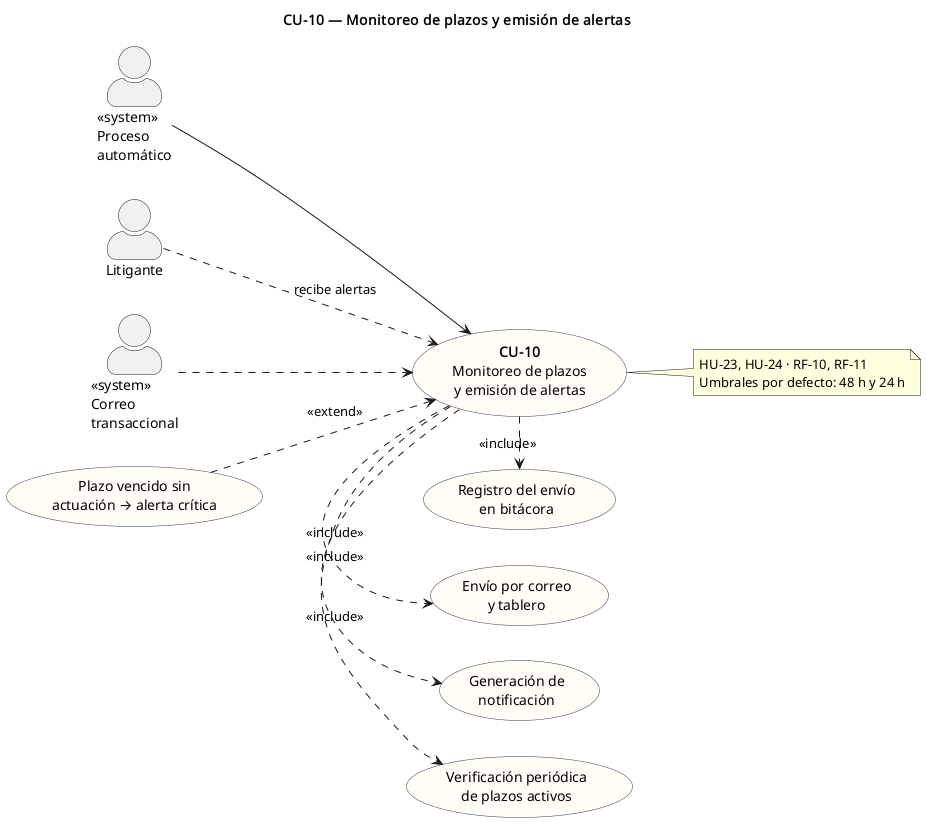
\includegraphics[width=0.9\linewidth]{image14.png}
  \caption{Diagrama CU-10. Monitoreo de plazos y emisión de alertas.}
  \label{fig:cu-10}
\end{figure}

\subsection{Gestión Documental y Cadena de Custodia}\label{sec:cu-documental}

\subsubsection{CU-11 --- Carga y clasificación de documentos}

\begin{table}[H]
  \centering
  \caption{Caso de uso CU-11: Carga y clasificación de documentos.}
  \label{tab:cu-11}
  \begin{tabularx}{\linewidth}{@{}>{\bfseries}l X@{}}
    \toprule
    ID & \textbf{CU-11} \\
    \midrule
    Nombre & Carga y clasificación de documentos \\
    Actor principal & Litigante \\
    Actores secundarios & Paralegal (consulta posterior) \\
    Precondiciones & Existe un expediente al cual asociar el documento. El usuario tiene perfil con permisos de carga. \\
    Flujo principal & 1. El Litigante accede al repositorio documental del expediente. 2. Selecciona el archivo a cargar (PDF, DOCX u otro formato admitido). 3. Asigna tipo documental, clasificación y etiquetas al documento. 4. El sistema calcula la huella digital del archivo al momento de la carga. 5. El sistema cifra el documento y lo almacena en el repositorio. 6. El sistema registra en la cadena de custodia: tipo de operación (carga), usuario responsable, marca de tiempo, huella digital del documento y estado del documento. \\
    Flujos alternos & 2a. El formato del archivo no está admitido → el sistema rechaza la carga e informa los formatos permitidos. 2b. El archivo excede el tamaño máximo admitido → el sistema rechaza la carga. \\
    Postcondiciones & El documento queda almacenado cifrado, indexado con su huella digital y disponible para consulta por los perfiles autorizados. La operación queda registrada en la cadena de custodia. \\
    Derivado de & HU-25, HU-26, HU-28, HU-30, HU-32 \\
    RF relacionados & RF-12, RF-13, RF-14 \\
    RNF relacionados & RNF-03, RNF-04 \\
    \bottomrule
  \end{tabularx}
\end{table}

\begin{figure}[H]
  \centering
  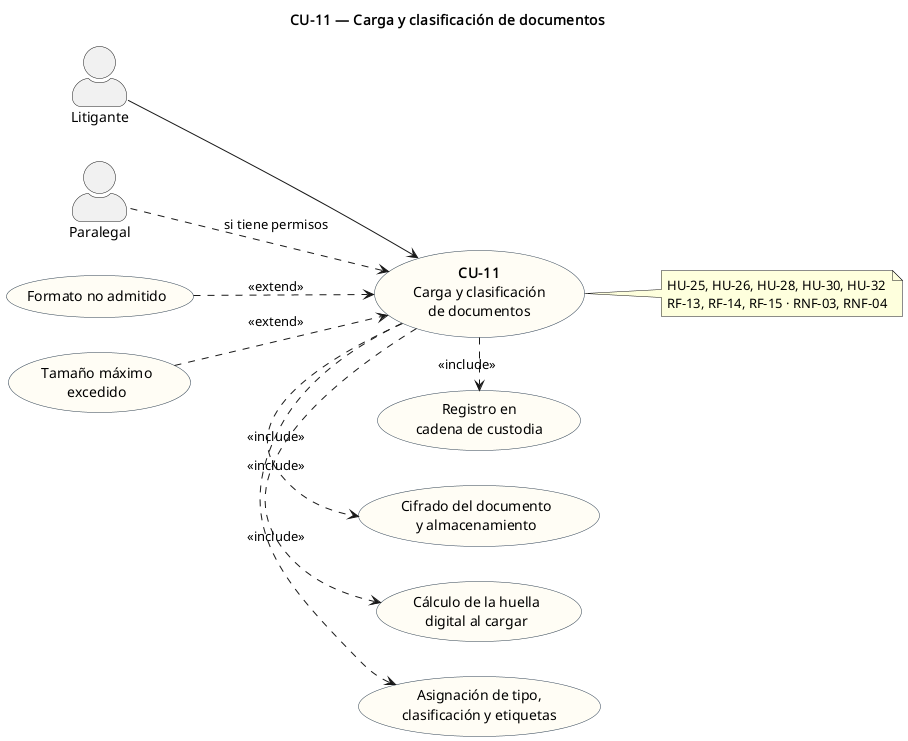
\includegraphics[width=0.9\linewidth]{image15.png}
  \caption{Diagrama CU-11. Carga y clasificación de documentos.}
  \label{fig:cu-11}
\end{figure}

\subsubsection{CU-12 --- Consulta de documentos con verificación de integridad}

\begin{table}[H]
  \centering
  \caption{Caso de uso CU-12: Consulta de documentos con verificación de integridad.}
  \label{tab:cu-12}
  \begin{tabularx}{\linewidth}{@{}>{\bfseries}l X@{}}
    \toprule
    ID & \textbf{CU-12} \\
    \midrule
    Nombre & Consulta de documentos con verificación de integridad \\
    Actor principal & Litigante o Paralegal \\
    Actores secundarios & --- \\
    Precondiciones & El usuario tiene perfil con acceso al expediente que contiene el documento. \\
    Flujo principal & 1. El usuario accede al repositorio documental del expediente. 2. Selecciona el documento a consultar. 3. El sistema verifica que el perfil del usuario tiene permiso de acceso al expediente. 4. El sistema descifra el documento. 5. El sistema recalcula la huella digital del documento descifrado y la compara con el valor de referencia almacenado al momento de la carga. 6. Si las huellas coinciden, el sistema entrega el documento al usuario. 7. La operación de consulta se registra en la cadena de custodia. \\
    Flujos alternos & 3a. El usuario no tiene permiso sobre el expediente → el sistema deniega el acceso. 4a. La verificación de la etiqueta de autenticación del cifrado falla (el contenido cifrado fue manipulado en el almacenamiento) → el sistema rechaza el descifrado, notifica al usuario y al Owner, y registra el incidente como alerta de seguridad. 5a. La huella digital recalculada no coincide con la referencia → el sistema alerta al usuario de que el documento fue modificado, bloquea la entrega y registra la discrepancia. \\
    Postcondiciones & El usuario recibe el documento íntegro, o recibe una alerta explícita de alteración. La consulta y su resultado quedan registrados en la cadena de custodia. \\
    Derivado de & HU-27, HU-29, HU-31, HU-33 \\
    RF relacionados & RF-11, RF-12, RF-13, RF-14 \\
    RNF relacionados & RNF-03, RNF-04 \\
    \bottomrule
  \end{tabularx}
\end{table}

\begin{figure}[H]
  \centering
  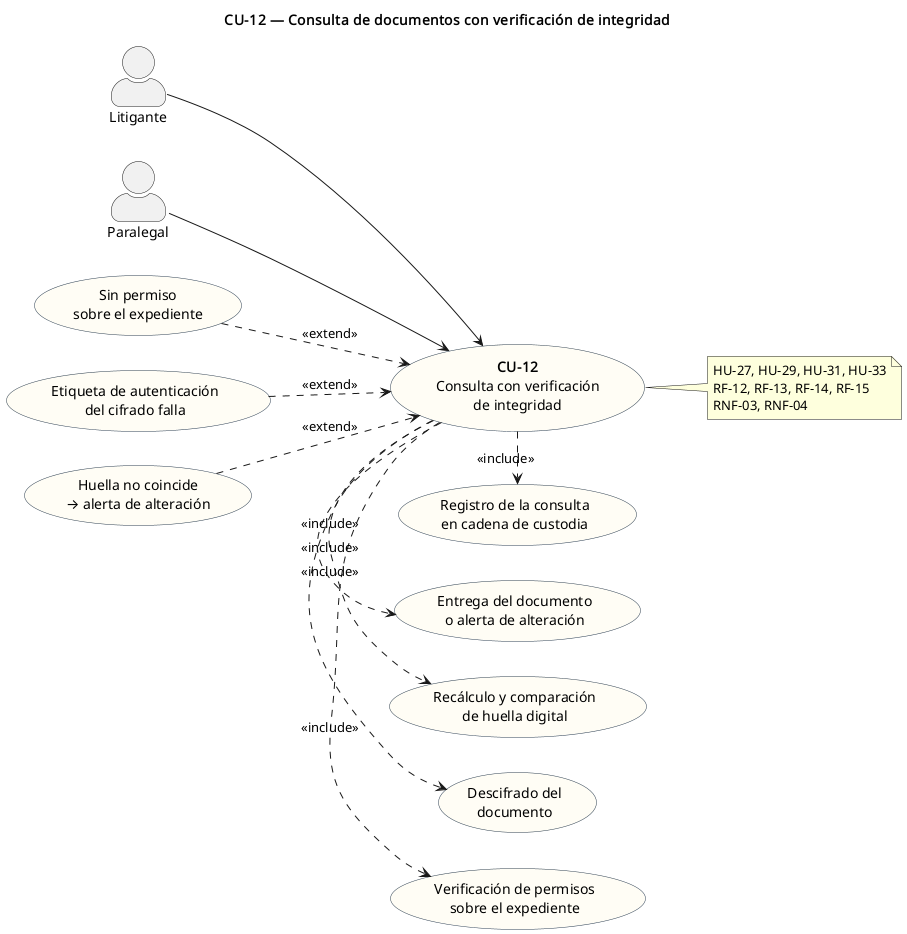
\includegraphics[width=0.9\linewidth]{image16.png}
  \caption{Diagrama CU-12. Consulta de documentos con verificación de integridad.}
  \label{fig:cu-12}
\end{figure}

\subsection{Firma de Contratos y Constancia de Fecha}\label{sec:cu-firma}

\subsubsection{CU-13 --- Firma digital de contrato con sellado de tiempo}

\begin{table}[H]
  \centering
  \caption{Caso de uso CU-13: Firma digital de contrato con sellado de tiempo.}
  \label{tab:cu-13}
  \begin{tabularx}{\linewidth}{@{}>{\bfseries}l X@{}}
    \toprule
    ID & \textbf{CU-13} \\
    \midrule
    Nombre & Firma digital de contrato con sellado de tiempo \\
    Actor principal & Litigante (firmante) \\
    Actores secundarios & TSA configurada (autoridad local en la demostración; PSC autorizado solo en una integración futura) \\
    Precondiciones & El contrato existe en el repositorio en formato PDF y está listo para firma. El firmante tiene un certificado digital X.509 vigente registrado en el sistema. \\
    Flujo principal & 1. El Litigante accede al contrato y selecciona la opción de firma digital. 2. El sistema presenta el contenido del contrato y solicita confirmación explícita de la acción de firma. 3. El Litigante confirma la firma. 4. El sistema calcula la huella digital del contrato. 5. El sistema firma la huella digital con la clave privada del certificado X.509 del firmante, vinculando criptográficamente su identidad con el contenido del documento. 6. El sistema envía la huella digital a la TSA configurada mediante el protocolo de sellado de tiempo. 7. La TSA retorna el token RFC 3161 que acredita criptográficamente el digest y su tiempo de generación. 8. El sistema almacena el contrato firmado junto con la firma digital, los metadatos del certificado y el token de sello de tiempo. 9. La operación se registra en la bitácora de actividad y en la cadena de custodia del expediente. \\
    Flujos alternos & 2a. El certificado del firmante ha expirado o está revocado → el sistema informa la situación e impide la firma. 6a. La TSA no responde dentro del tiempo límite → el sistema informa o encola la solicitud según la política explícita del emisor; no conmuta silenciosamente a otra autoridad. 7a. El token recibido no supera la validación de formato → el sistema rechaza el sello y registra el error. \\
    Postcondiciones & El contrato queda firmado con evidencia criptográfica verificable de la identidad del firmante y del momento de la firma. Si la autoridad es la TSA local, el resultado acredita el flujo técnico RFC 3161, pero no constituye por sí mismo una constancia NOM-151 de un PSC autorizado. \\
    Derivado de & HU-34, HU-35 \\
    RF relacionados & RF-15, RF-16 \\
    RNF relacionados & RNF-03, RNF-11 \\
    \bottomrule
  \end{tabularx}
\end{table}

\begin{figure}[H]
  \centering
  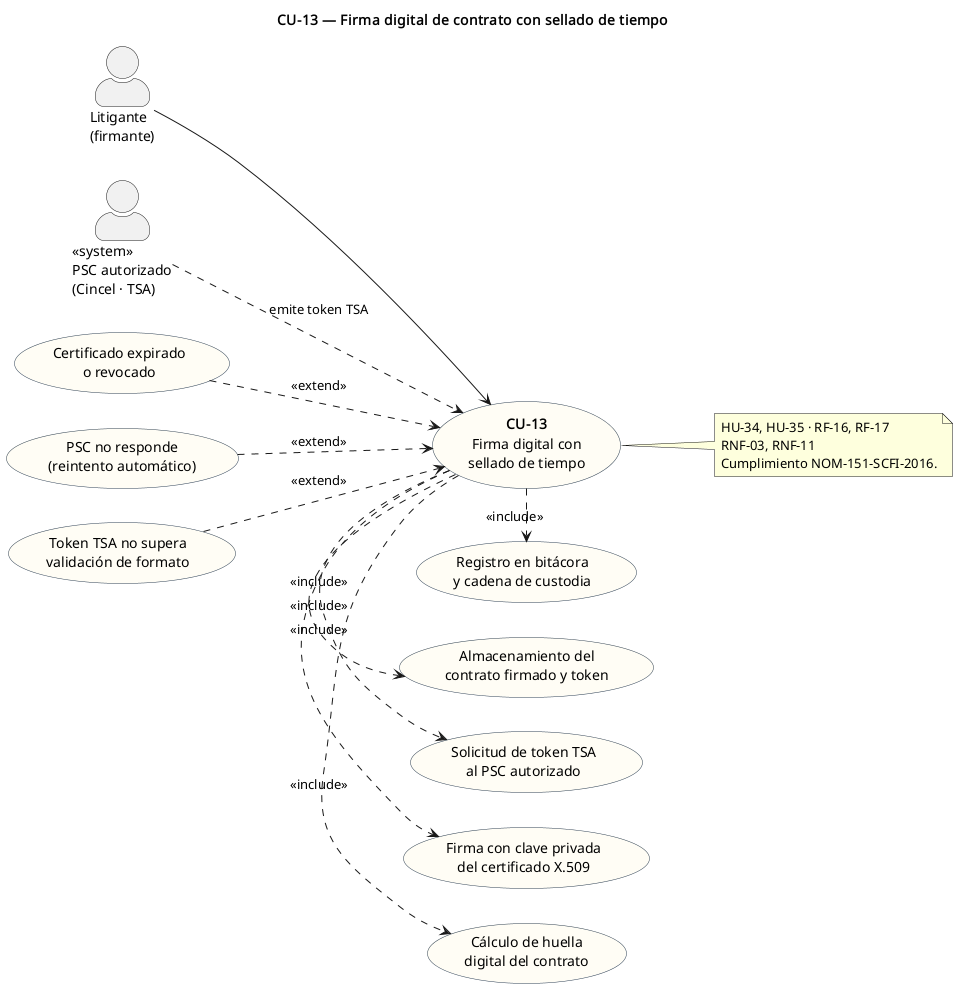
\includegraphics[width=0.9\linewidth]{image17.png}
  \caption{Diagrama CU-13. Firma digital de contrato con sellado de tiempo.}
  \label{fig:cu-13}
\end{figure}

\subsubsection{CU-14 --- Verificación de firma digital y sello de tiempo}

\begin{table}[H]
  \centering
  \caption{Caso de uso CU-14: Verificación de firma digital y sello de tiempo.}
  \label{tab:cu-14}
  \begin{tabularx}{\linewidth}{@{}>{\bfseries}l X@{}}
    \toprule
    ID & \textbf{CU-14} \\
    \midrule
    Nombre & Verificación de firma digital y sello de tiempo \\
    Actor principal & Usuario autenticado con acceso al contrato \\
    Actores secundarios & --- \\
    Precondiciones & El contrato ha sido firmado digitalmente y posee un token de sello de tiempo asociado. \\
    Flujo principal & 1. El usuario accede al contrato firmado y selecciona la opción de verificación. 2. El sistema recalcula la huella digital del contrato actual. 3. El sistema verifica la firma digital: descifra la firma con la clave pública del certificado X.509 del firmante y compara el resultado con la huella digital recalculada. 4. El sistema valida el estado del certificado del firmante (vigente, revocado o expirado) consultando la cadena de certificación. 5. El sistema verifica la autenticidad del token de sello de tiempo validando la firma del PSC. 6. El sistema presenta al usuario un reporte de verificación con el resultado de cada componente. \\
    Flujos alternos & 3a. La huella digital recalculada no coincide con la contenida en la firma → el sistema reporta que el documento fue modificado después de firmado e indica la causa de la invalidación. 4a. El certificado del firmante ha expirado o fue revocado → el sistema lo indica en el reporte sin invalidar necesariamente la firma (la firma era válida al momento del sellado). 5a. El token de sello de tiempo no supera la validación → el sistema reporta que la constancia de fecha no es verificable. \\
    Postcondiciones & El usuario dispone de un reporte de verificación con el estado de cada componente: validez de la firma, estado del certificado, validez del sello de tiempo e integridad del documento. \\
    Derivado de & HU-36, HU-37 \\
    RF relacionados & RF-17 \\
    RNF relacionados & RNF-11 \\
    \bottomrule
  \end{tabularx}
\end{table}

\begin{figure}[H]
  \centering
  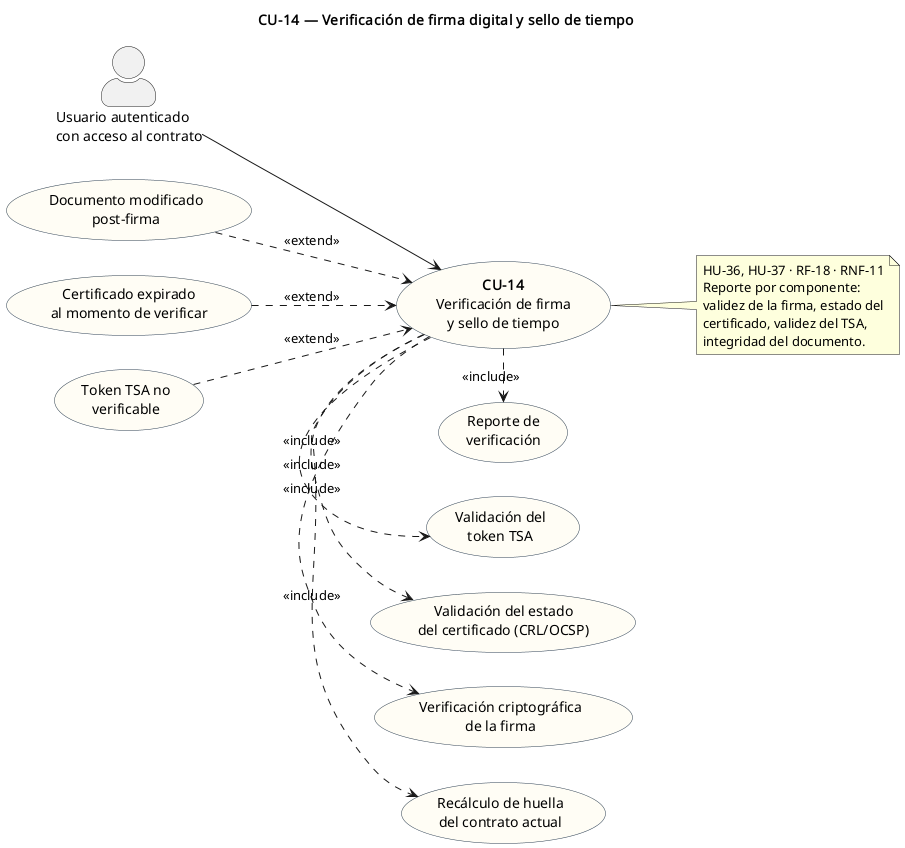
\includegraphics[width=0.9\linewidth]{image18.png}
  \caption{Diagrama CU-14. Verificación de firma digital y sello de tiempo.}
  \label{fig:cu-14}
\end{figure}

\subsection{Operación y Monitoreo}\label{sec:cu-operacion}

\subsubsection{CU-15 --- Consulta del tablero de control}

\begin{table}[H]
  \centering
  \caption{Caso de uso CU-15: Consulta del tablero de control.}
  \label{tab:cu-15}
  \begin{tabularx}{\linewidth}{@{}>{\bfseries}l X@{}}
    \toprule
    ID & \textbf{CU-15} \\
    \midrule
    Nombre & Consulta del tablero de control \\
    Actor principal & Owner o Litigante \\
    Actores secundarios & --- \\
    Precondiciones & El usuario tiene sesión activa. \\
    Flujo principal & 1. El usuario accede al tablero de control del despacho. 2. El sistema consulta los indicadores operativos del despacho: casos activos, plazos por vencer en 48 h y 7 días, contratos pendientes de firma y carga de trabajo por abogado. 3. El sistema presenta los indicadores con diferenciación visual por nivel de urgencia. \\
    Flujos alternos & 2a. Existen plazos fatales por vencer en menos de 48 horas → el sistema los destaca con indicador de alerta de nivel crítico, diferenciado visualmente del resto de elementos. \\
    Postcondiciones & El usuario visualiza el estado actual del despacho. \\
    Derivado de & HU-38 \\
    RF relacionados & RF-18 \\
    RNF relacionados & RNF-07 \\
    \bottomrule
  \end{tabularx}
\end{table}

\begin{figure}[H]
  \centering
  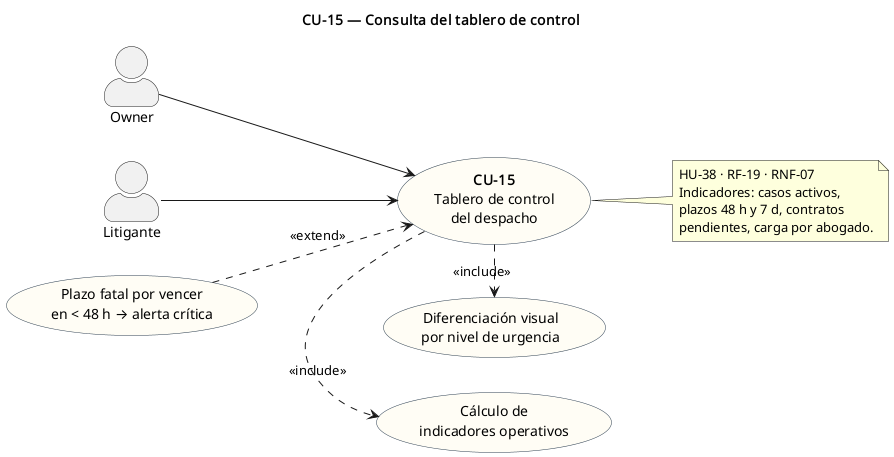
\includegraphics[width=0.9\linewidth]{image19.png}
  \caption{Diagrama CU-15. Consulta del tablero de control.}
  \label{fig:cu-15}
\end{figure}

\subsubsection{CU-16 --- Generación de informes}

\begin{table}[H]
  \centering
  \caption{Caso de uso CU-16: Generación de informes.}
  \label{tab:cu-16}
  \begin{tabularx}{\linewidth}{@{}>{\bfseries}l X@{}}
    \toprule
    ID & \textbf{CU-16} \\
    \midrule
    Nombre & Generación de informes \\
    Actor principal & Owner \\
    Actores secundarios & Sistema de colas de trabajo \\
    Precondiciones & El Owner tiene sesión activa. \\
    Flujo principal & 1. El Owner accede al módulo de reportes. 2. Selecciona el tipo de informe y los filtros aplicables (rango de fechas, abogado responsable, estado de los casos). 3. El sistema encola la solicitud de generación como tarea en segundo plano. 4. El sistema confirma la recepción de la solicitud y muestra un indicador de progreso. 5. Al completar la generación, el sistema notifica al Owner y pone el informe disponible para descarga en formato PDF o CSV. \\
    Flujos alternos & 3a. El volumen de datos supera el umbral de procesamiento inmediato → el sistema informa el tiempo estimado y envía notificación por correo cuando el reporte esté listo. \\
    Postcondiciones & El informe queda disponible para descarga. La interfaz permanece responsiva durante el procesamiento. \\
    Derivado de & HU-39 \\
    RF relacionados & RF-19 \\
    RNF relacionados & RNF-06, RNF-07 \\
    \bottomrule
  \end{tabularx}
\end{table}

\begin{figure}[H]
  \centering
  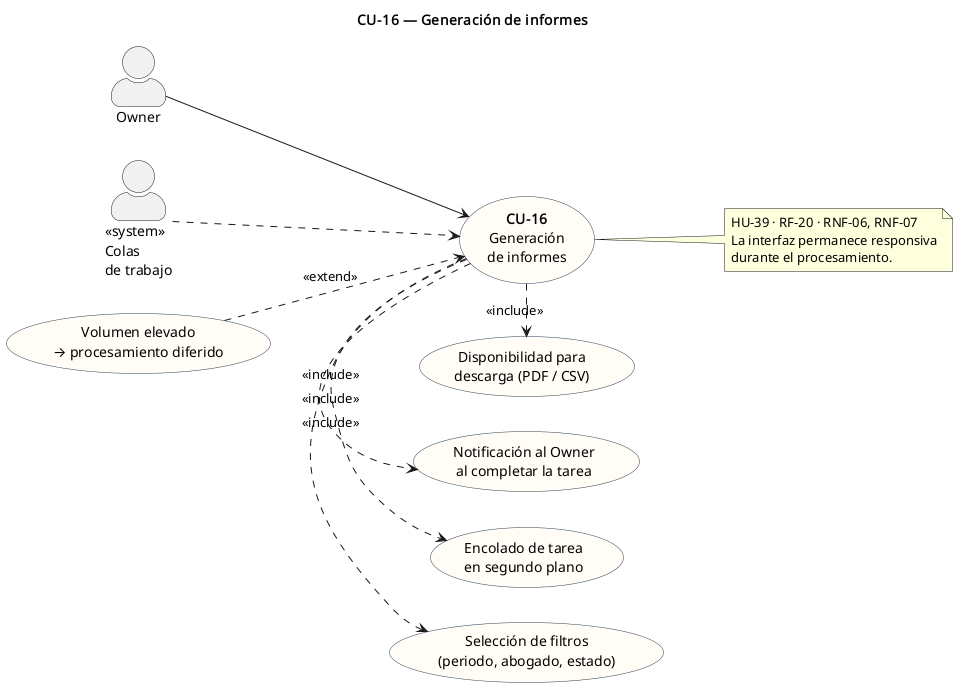
\includegraphics[width=0.9\linewidth]{image20.png}
  \caption{Diagrama CU-16. Generación de informes.}
  \label{fig:cu-16}
\end{figure}

\subsubsection{CU-17 --- Consulta de bitácora de actividad}

\begin{table}[H]
  \centering
  \caption{Caso de uso CU-17: Consulta de bitácora de actividad.}
  \label{tab:cu-17}
  \begin{tabularx}{\linewidth}{@{}>{\bfseries}l X@{}}
    \toprule
    ID & \textbf{CU-17} \\
    \midrule
    Nombre & Consulta de bitácora de actividad \\
    Actor principal & Owner \\
    Actores secundarios & --- \\
    Precondiciones & El Owner tiene sesión activa. \\
    Flujo principal & 1. El Owner accede al módulo de bitácora de actividad. 2. Aplica filtros de búsqueda (rango de fechas, usuario, tipo de operación, recurso afectado). 3. El sistema presenta los registros cronológicamente, mostrando para cada entrada: identificador del usuario, tipo de operación, recurso afectado, marca de tiempo y dirección IP. \\
    Flujos alternos & --- (la bitácora es de solo lectura; no existen operaciones de modificación o eliminación). \\
    Postcondiciones & El Owner visualiza los registros solicitados. Los registros de la bitácora no pueden modificarse ni eliminarse por ningún usuario del sistema, incluido el Owner. \\
    Derivado de & HU-40 \\
    RF relacionados & RF-20 \\
    RNF relacionados & RNF-04 \\
    \bottomrule
  \end{tabularx}
\end{table}

\begin{figure}[H]
  \centering
  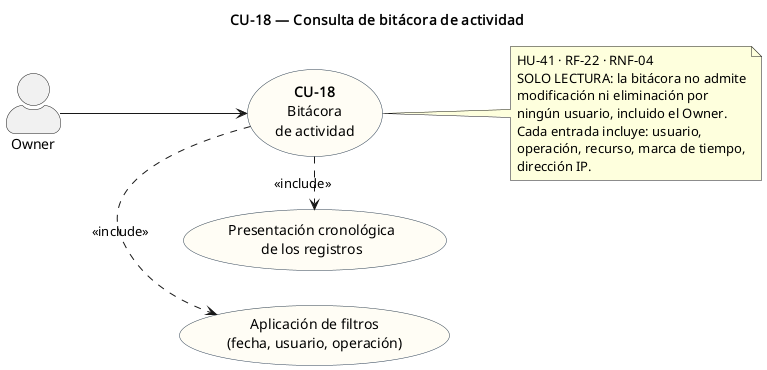
\includegraphics[width=0.9\linewidth]{image22.png}
  \caption{Diagrama CU-17. Consulta de bitácora de actividad.}
  \label{fig:cu-17}
\end{figure}


\section{Requerimientos del Sistema}\label{sec:requerimientos}

Los requerimientos se derivan de los objetivos definidos anteriormente y se organizan en funcionales y no funcionales. Los requerimientos funcionales definen los servicios que el sistema debe proporcionar y cómo debe reaccionar ante entradas particulares. Los requerimientos no funcionales describen restricciones y atributos de calidad que limitan las decisiones de diseño e implementación.

\subsection{Requerimientos Funcionales}\label{sec:requerimientos-funcionales}

Los requerimientos funcionales especifican los servicios que el sistema debe proporcionar, las entradas que acepta, las salidas que produce y el comportamiento esperado ante condiciones particulares. Cada requerimiento se deriva de las historias de usuario definidas en la \cref{sec:historias-usuario} y se formaliza mediante una estructura que incluye descripción, entradas, salidas, actores involucrados y criterio de aceptación verificable. Los requerimientos se agrupan en cinco categorías funcionales alineadas con los módulos del prototipo.

\subsubsection{Autenticación y Control de Acceso}

\begin{table}[H]
  \centering
  \caption{RF-01: Autenticación y gestión de sesiones}
  \label{tab:rf-01}
  \begin{tabularx}{\linewidth}{@{}L{3.2cm}X@{}}
    \toprule
    \textbf{ID} & RF-01 \\
    \midrule
    \textbf{Nombre} & Autenticación y gestión de sesiones \\
    \textbf{Descripción} & El sistema debe proveer mecanismos seguros de inicio de sesión, recuperación de contraseñas, expiración de sesiones por inactividad y protección contra fijación de sesión. \\
    \textbf{Entrada} & Credenciales del usuario (usuario/contraseña o certificado digital); solicitud de recuperación de contraseña. \\
    \textbf{Salida} & Sesión autenticada con token de acceso; notificación de expiración; redireccionamiento al inicio de sesión tras inactividad sin pérdida de datos no guardados. \\
    \textbf{Actores involucrados} & Todos los roles (Owner, Litigante, Paralegal, Cliente); sistema de gestión de sesiones. \\
    \textbf{Criterio de aceptación} & Dado un usuario inactivo por el tiempo configurado, cuando vence la sesión, entonces el sistema la invalida automáticamente y requiere nueva autenticación sin pérdida de datos no guardados. \\
    \bottomrule
  \end{tabularx}
\end{table}

\begin{table}[H]
  \centering
  \caption{RF-02: Control de acceso basado en roles (RBAC)}
  \label{tab:rf-02}
  \begin{tabularx}{\linewidth}{@{}L{3.2cm}X@{}}
    \toprule
    \textbf{ID} & RF-02 \\
    \midrule
    \textbf{Nombre} & Control de acceso basado en roles (RBAC) \\
    \textbf{Descripción} & El sistema debe asignar permisos de forma granular a través de roles predefinidos (Owner, Litigante, Paralegal, Cliente) para restringir el acceso a módulos y operaciones sensibles. \\
    \textbf{Entrada} & Rol asignado al usuario; recurso o módulo al que se intenta acceder. \\
    \textbf{Salida} & Permiso concedido o denegado; registro en bitácora del intento de acceso. \\
    \textbf{Actores involucrados} & Owner (configuración de roles); todos los usuarios como sujetos de control; sistema de autorización. \\
    \textbf{Criterio de aceptación} & Dado un usuario con rol Paralegal, cuando intenta acceder a un módulo restringido a Owner o Litigante, entonces el sistema deniega el acceso con mensaje explicativo y registra el intento en la bitácora. \\
    \bottomrule
  \end{tabularx}
\end{table}

\begin{table}[H]
  \centering
  \caption{RF-03: Gestión de equipos colaborativos}
  \label{tab:rf-03}
  \begin{tabularx}{\linewidth}{@{}L{3.2cm}X@{}}
    \toprule
    \textbf{ID} & RF-03 \\
    \midrule
    \textbf{Nombre} & Gestión de equipos colaborativos \\
    \textbf{Descripción} & El sistema debe permitir invitar nuevos miembros al despacho mediante correo electrónico, gestionar la aceptación de invitaciones y administrar el alta y baja de usuarios en el equipo. \\
    \textbf{Entrada} & Correo electrónico del nuevo miembro; rol a asignar; acción de aceptación del invitado. \\
    \textbf{Salida} & Invitación enviada; usuario creado y asociado al despacho; acceso habilitado según el rol asignado. \\
    \textbf{Actores involucrados} & Owner (invita y da de baja); usuario invitado; sistema de correo transaccional. \\
    \textbf{Criterio de aceptación} & Dado un Owner que envía una invitación, cuando el invitado la acepta dentro del periodo de validez del enlace, entonces queda registrado con el rol indicado; si el enlace vence, la invitación queda inactiva automáticamente. \\
    \bottomrule
  \end{tabularx}
\end{table}

\subsubsection{Gestión Procesal Penal}

\begin{table}[H]
  \centering
  \caption{RF-04: Expediente penal digital}
  \label{tab:rf-04}
  \begin{tabularx}{\linewidth}{@{}L{3.2cm}X@{}}
    \toprule
    \textbf{ID} & RF-04 \\
    \midrule
    \textbf{Nombre} & Expediente penal digital \\
    \textbf{Descripción} & El sistema debe permitir el registro y administración integral de casos penales, incluyendo identificadores oficiales (NUC, Carpeta Judicial), delitos y metadatos asociados. \\
    \textbf{Entrada} & NUC, Carpeta Judicial, tipo de delito, datos del caso y metadatos ingresados por el Litigante. \\
    \textbf{Salida} & Expediente registrado con identificadores únicos, estado inicial `Investigación' y timestamp de creación. \\
    \textbf{Actores involucrados} & Litigante, Paralegal; base de datos relacional. \\
    \textbf{Criterio de aceptación} & Dado un Litigante que registra un nuevo caso, cuando omite el NUC o la Carpeta Judicial, entonces el sistema rechaza el registro con indicación del campo faltante; cuando los datos son completos, el expediente queda persistido y disponible en el módulo de gestión procesal. \\
    \bottomrule
  \end{tabularx}
\end{table}

\begin{table}[H]
  \centering
  \caption{RF-05: Control de etapas procesales (CNPP)}
  \label{tab:rf-05}
  \begin{tabularx}{\linewidth}{@{}L{3.2cm}X@{}}
    \toprule
    \textbf{ID} & RF-05 \\
    \midrule
    \textbf{Nombre} & Control de etapas procesales (CNPP) \\
    \textbf{Descripción} & El sistema debe gestionar la transición entre etapas procesales (Investigación, Intermedia, Juicio Oral) conforme al CNPP, manteniendo un historial inmutable de cambios y validaciones procesales. \\
    \textbf{Entrada} & Documento procesal habilitante cargado por el usuario (ej. escrito de acusación para transitar de Investigación a Intermedia). \\
    \textbf{Salida} & Registro inmutable de la transición con marca de tiempo, identificador de usuario y documento asociado; módulo de la siguiente etapa habilitado. \\
    \textbf{Actores involucrados} & Litigante (Owner); sistema de gestión procesal; bitácora de auditoría. \\
    \textbf{Criterio de aceptación} & Dado un expediente en etapa de Investigación, cuando se intenta avanzar sin cargar el escrito de acusación, entonces el sistema rechaza la transición; cuando se carga el documento habilitante, la transición se registra de forma inmutable y no puede revertirse. \\
    \bottomrule
  \end{tabularx}
\end{table}

\begin{table}[H]
  \centering
  \caption{RF-06: Directorio de participantes}
  \label{tab:rf-06}
  \begin{tabularx}{\linewidth}{@{}L{3.2cm}X@{}}
    \toprule
    \textbf{ID} & RF-06 \\
    \midrule
    \textbf{Nombre} & Directorio de participantes \\
    \textbf{Descripción} & El sistema debe permitir la gestión de sujetos procesales vinculados a cada caso (imputados, víctimas, jueces, peritos), definiendo su rol procesal y estatus jurídico. \\
    \textbf{Entrada} & Datos del sujeto procesal (nombre, rol, cédula, CURP u otros identificadores según tipo); caso al que se vincula. \\
    \textbf{Salida} & Participante registrado y vinculado al expediente con su rol procesal; historial de cambios de rol disponible. \\
    \textbf{Actores involucrados} & Litigante; sistema de gestión de directorio. \\
    \textbf{Criterio de aceptación} & Dado un caso activo, cuando se registra un participante con rol `Juez de control', entonces el sistema valida que se proporcione el órgano jurisdiccional y la firma electrónica (FIREL); un mismo usuario puede tener roles distintos en casos diferentes sin conflicto. \\
    \bottomrule
  \end{tabularx}
\end{table}

\begin{table}[H]
  \centering
  \caption{RF-07: Gestión de audiencias especializadas}
  \label{tab:rf-07}
  \begin{tabularx}{\linewidth}{@{}L{3.2cm}X@{}}
    \toprule
    \textbf{ID} & RF-07 \\
    \midrule
    \textbf{Nombre} & Gestión de audiencias especializadas \\
    \textbf{Descripción} & El sistema debe permitir la programación y seguimiento de audiencias tipificadas según el CNPP, registrando resultados, asistentes y acuerdos derivados. \\
    \textbf{Entrada} & Tipo de audiencia (del catálogo CNPP), fecha, hora, participantes y modalidad (presencial o videoconferencia). \\
    \textbf{Salida} & Audiencia agendada vinculada al expediente; activación automática del cómputo de plazos derivados; registro de resultados y acuerdos. \\
    \textbf{Actores involucrados} & Litigante; sistema de calendario; módulo de plazos. \\
    \textbf{Criterio de aceptación} & Dado el registro de una `Audiencia inicial' con vinculación a proceso, cuando se confirma, entonces el sistema activa automáticamente el plazo de investigación complementaria (2 o 6 meses) y genera la alerta preventiva correspondiente. \\
    \bottomrule
  \end{tabularx}
\end{table}

\begin{table}[H]
  \centering
  \caption{RF-08: Blindaje de plazos procesales}
  \label{tab:rf-08}
  \begin{tabularx}{\linewidth}{@{}L{3.2cm}X@{}}
    \toprule
    \textbf{ID} & RF-08 \\
    \midrule
    \textbf{Nombre} & Blindaje de plazos procesales \\
    \textbf{Descripción} & El sistema debe permitir el registro y cálculo de términos constitucionales y plazos fatales, con derivación automática a partir de actuaciones o audiencias registradas. \\
    \textbf{Entrada} & Actuación o audiencia registrada que activa un plazo constitucional; calendario de días inhábiles configurado por entidad federativa. \\
    \textbf{Salida} & Plazo calculado con fecha y hora de vencimiento; alerta programada; registro en el módulo de plazos del expediente. \\
    \textbf{Actores involucrados} & Litigante; sistema de cómputo de plazos; calendario judicial configurable. \\
    \textbf{Criterio de aceptación} & Dado el registro de vinculación a proceso con plazo de 6 meses de investigación complementaria, entonces el sistema calcula la fecha de vencimiento excluyendo correctamente los días inhábiles del calendario configurado para la entidad federativa correspondiente. \\
    \bottomrule
  \end{tabularx}
\end{table}

\begin{table}[H]
  \centering
  \caption{RF-09: Sistema de alertas preventivas}
  \label{tab:rf-09}
  \begin{tabularx}{\linewidth}{@{}L{3.2cm}X@{}}
    \toprule
    \textbf{ID} & RF-09 \\
    \midrule
    \textbf{Nombre} & Sistema de alertas preventivas \\
    \textbf{Descripción} & El sistema debe generar notificaciones automáticas ante la proximidad de vencimientos de plazos o audiencias programadas. \\
    \textbf{Entrada} & Plazos activos registrados; reglas de anticipación configurables (ej. alerta a 48 h y a 24 h del vencimiento). \\
    \textbf{Salida} & Notificación enviada al Litigante responsable por correo y visible en el dashboard del sistema. \\
    \textbf{Actores involucrados} & Litigante; sistema de notificaciones; módulo de colas de trabajo. \\
    \textbf{Criterio de aceptación} & Dado un plazo de vinculación a proceso con vencimiento en 48 horas, cuando el sistema ejecuta la verificación periódica de plazos, entonces envía una notificación de alerta roja al Litigante responsable; el envío se registra en la bitácora. \\
    \bottomrule
  \end{tabularx}
\end{table}

\begin{table}[H]
  \centering
  \caption{RF-10: Calendario jurídico integrado}
  \label{tab:rf-10}
  \begin{tabularx}{\linewidth}{@{}L{3.2cm}X@{}}
    \toprule
    \textbf{ID} & RF-10 \\
    \midrule
    \textbf{Nombre} & Calendario jurídico integrado \\
    \textbf{Descripción} & El sistema debe proveer una visualización unificada de la agenda del despacho, integrando audiencias y plazos límite en un calendario interactivo. \\
    \textbf{Entrada} & Audiencias programadas; plazos activos; configuración de la vista seleccionada (día, semana o mes). \\
    \textbf{Salida} & Calendario unificado con codificación de color por tipo de evento y acceso directo al expediente relacionado desde cada entrada. \\
    \textbf{Actores involucrados} & Litigante, Paralegal, Owner. \\
    \textbf{Criterio de aceptación} & Dado un despacho con 5 o más casos activos, cuando el Litigante accede al calendario, entonces visualiza todos los vencimientos y audiencias de sus casos en una sola vista sin necesidad de navegar por cada expediente individualmente. \\
    \bottomrule
  \end{tabularx}
\end{table}

\subsubsection{Gestión Documental y Evidencias}

\begin{table}[H]
  \centering
  \caption{RF-11: Cadena de custodia digital}
  \label{tab:rf-11}
  \begin{tabularx}{\linewidth}{@{}L{3.2cm}X@{}}
    \toprule
    \textbf{ID} & RF-11 \\
    \midrule
    \textbf{Nombre} & Cadena de custodia digital \\
    \textbf{Descripción} & El sistema debe proveer un módulo para el registro de evidencias físicas y digitales, garantizando la trazabilidad de sus movimientos y resguardos mediante un registro cronológico inmutable. \\
    \textbf{Entrada} & Evidencia física o digital ingresada al sistema; operación de movimiento o consulta de la evidencia. \\
    \textbf{Salida} & Registro cronológico append-only con: tipo de operación, identificador de la evidencia, usuario responsable, timestamp y estado de la evidencia. \\
    \textbf{Actores involucrados} & Litigante, Paralegal; sistema de almacenamiento NoSQL (registro de auditoría). \\
    \textbf{Criterio de aceptación} & Dado un registro de evidencia existente, cuando cualquier usuario intenta modificar o eliminar una entrada de la cadena de custodia, entonces el sistema rechaza la operación; cada nuevo movimiento genera únicamente un registro de inserción nuevo. \\
    \bottomrule
  \end{tabularx}
\end{table}

\begin{table}[H]
  \centering
  \caption{RF-12: Repositorio documental}
  \label{tab:rf-12}
  \begin{tabularx}{\linewidth}{@{}L{3.2cm}X@{}}
    \toprule
    \textbf{ID} & RF-12 \\
    \midrule
    \textbf{Nombre} & Repositorio documental \\
    \textbf{Descripción} & El sistema debe permitir cargar, clasificar, consultar y compartir documentos procesales asociados a expedientes, asegurando su organización, disponibilidad y control de versiones. \\
    \textbf{Entrada} & Archivo digital (PDF, DOCX, multimedia); clasificación y metadatos ingresados por el usuario; expediente al que se asocia. \\
    \textbf{Salida} & Documento almacenado cifrado (AES-256-GCM), indexado con su hash SHA-256 y disponible para consulta por los roles autorizados. \\
    \textbf{Actores involucrados} & Litigante, Paralegal; sistema de almacenamiento cifrado. \\
    \textbf{Criterio de aceptación} & Dado un documento cargado al repositorio, cuando un Paralegal intenta acceder a un documento de un expediente no asignado, entonces el sistema deniega el acceso; el documento debe ser recuperable en menos de 3 segundos para archivos de hasta 10 MB. \\
    \bottomrule
  \end{tabularx}
\end{table}

\subsubsection{Servicios Criptográficos}

\begin{table}[H]
  \centering
  \caption{RF-13: Verificación de integridad de documentos}
  \label{tab:rf-13}
  \begin{tabularx}{\linewidth}{@{}L{3.2cm}X@{}}
    \toprule
    \textbf{ID} & RF-13 \\
    \midrule
    \textbf{Nombre} & Verificación de integridad de documentos \\
    \textbf{Descripción} & El sistema debe calcular y almacenar el hash SHA-256 (véase §2.3.1) de cada documento al momento de su carga. En cada consulta posterior, debe recalcular el hash y compararlo con el valor de referencia, notificando al usuario si se detecta una discrepancia. \\
    \textbf{Entrada} & Archivo digital cargado al sistema (PDF, DOCX u otro formato admitido). \\
    \textbf{Salida} & Hash SHA-256 almacenado en base de datos; alerta visible al usuario en caso de discrepancia detectada en consulta posterior. \\
    \textbf{Actores involucrados} & Litigante, Paralegal; sistema de almacenamiento (backend). \\
    \textbf{Criterio de aceptación} & Dado un documento cargado, cuando se modifica 1 byte del archivo almacenado, entonces el sistema detecta la discrepancia y muestra una alerta en la siguiente consulta sin requerir intervención manual. \\
    \bottomrule
  \end{tabularx}
\end{table}

\begin{table}[H]
  \centering
  \caption{RF-14: Cifrado autenticado de expedientes y documentos}
  \label{tab:rf-14}
  \begin{tabularx}{\linewidth}{@{}L{3.2cm}X@{}}
    \toprule
    \textbf{ID} & RF-14 \\
    \midrule
    \textbf{Nombre} & Cifrado autenticado de expedientes y documentos \\
    \textbf{Descripción} & El sistema debe cifrar los documentos y expedientes almacenados mediante AES-256-GCM (véase §2.3.2), proveyendo simultáneamente confidencialidad e integridad. Cada operación de cifrado debe emplear un vector de inicialización (IV) único generado aleatoriamente. \\
    \textbf{Entrada} & Documento o expediente a cifrar; clave maestra del despacho; IV generado aleatoriamente por operación. \\
    \textbf{Salida} & Contenido cifrado con AES-256-GCM almacenado en el repositorio; IV almacenado de forma separada de los datos cifrados. \\
    \textbf{Actores involucrados} & Sistema de cifrado (backend); módulo de gestión de claves. \\
    \textbf{Criterio de aceptación} & Dado un documento cifrado almacenado, cuando se modifica 1 byte del texto cifrado directamente en el almacenamiento, entonces la verificación de la etiqueta de autenticación GCM falla y el sistema rechaza el descifrado; cada operación debe utilizar un IV único, verificable mediante pruebas TDD. \\
    \bottomrule
  \end{tabularx}
\end{table}

\begin{table}[H]
  \centering
  \caption{RF-15: Firma digital de contratos}
  \label{tab:rf-15}
  \begin{tabularx}{\linewidth}{@{}L{3.2cm}X@{}}
    \toprule
    \textbf{ID} & RF-15 \\
    \midrule
    \textbf{Nombre} & Firma digital de contratos \\
    \textbf{Descripción} & El sistema debe permitir la firma digital de contratos mediante certificados X.509 (véase §2.3.3), vinculando criptográficamente la identidad del firmante con el contenido del documento. \\
    \textbf{Entrada} & Contrato en formato PDF listo para firmar; certificado X.509 del firmante; confirmación de la acción de firma por el usuario. \\
    \textbf{Salida} & Documento firmado con hash SHA-256 cifrado con la clave privada del firmante; metadatos de firma (timestamp local, identificador del certificado) almacenados junto al documento. \\
    \textbf{Actores involucrados} & Litigante (firmante); sistema de firma digital; módulo de certificados X.509. \\
    \textbf{Criterio de aceptación} & Dado un contrato firmado digitalmente, cuando se modifica cualquier byte del documento posterior a la firma, entonces la verificación retorna inválida; la firma solo puede verificarse exitosamente con la clave pública del certificado X.509 del firmante. \\
    \bottomrule
  \end{tabularx}
\end{table}

\begin{table}[H]
  \centering
  \caption{RF-16: Sellado de tiempo (NOM-151)}
  \label{tab:rf-16}
  \begin{tabularx}{\linewidth}{@{}L{3.2cm}X@{}}
    \toprule
    \textbf{ID} & RF-16 \\
    \midrule
    \textbf{Nombre} & Sellado de tiempo (NOM-151) \\
    \textbf{Descripción} & El sistema debe obtener un token RFC 3161 para cada contrato firmado mediante la TSA configurada, acreditando criptográficamente la existencia del digest en un momento determinado. La constancia NOM-151 de un PSC autorizado no se afirma para la TSA local. \\
    \textbf{Entrada} & Hash SHA-256 del contrato firmado y solicitud al adaptador de TSA configurado. \\
    \textbf{Salida} & Token de sello de tiempo (TimeStampToken) en formato ASN.1/.tsr almacenado y vinculado al contrato; la naturaleza técnica o regulada del emisor queda identificada en el paquete. \\
    \textbf{Actores involucrados} & Sistema backend (cliente TSA); TSA local de demostración o PSC autorizado futuro; módulo de firma digital. \\
    \textbf{Criterio de aceptación} & Dado un contrato firmado, cuando se solicita el sello a la TSA configurada, el sistema almacena un token RFC 3161 que cubre el digest y puede verificarse de forma independiente con OpenSSL sin requerir acceso al sistema. La campaña de estabilidad de un PSC externo queda fuera del alcance actual. \\
    \bottomrule
  \end{tabularx}
\end{table}

\begin{table}[H]
  \centering
  \caption{RF-17: Verificación de firmas y sellos de tiempo}
  \label{tab:rf-17}
  \begin{tabularx}{\linewidth}{@{}L{3.2cm}X@{}}
    \toprule
    \textbf{ID} & RF-17 \\
    \midrule
    \textbf{Nombre} & Verificación de firmas y sellos de tiempo \\
    \textbf{Descripción} & El sistema debe permitir verificar la validez de las firmas digitales y los sellos de tiempo asociados a un contrato, incluyendo la cadena de certificados X.509, vigencia del certificado e integridad del documento. \\
    \textbf{Entrada} & Contrato firmado con su token de sello de tiempo; cadena de certificados X.509 del firmante. \\
    \textbf{Salida} & Resultado de verificación con detalle de: validez de la firma, estado del certificado (vigente/revocado/expirado), validez del sello de tiempo e integridad del documento. \\
    \textbf{Actores involucrados} & Cualquier usuario autenticado con acceso al contrato; sistema de verificación criptográfica. \\
    \textbf{Criterio de aceptación} & Dado un contrato con firma válida e integridad verificada, cuando se ejecuta la verificación, entonces todos los componentes se reportan como válidos; dado un contrato modificado, cuando se verifica, entonces el sistema reporta la firma como inválida con indicación explícita de la causa. \\
    \bottomrule
  \end{tabularx}
\end{table}

\subsubsection{Operación y Monitoreo}

\begin{table}[H]
  \centering
  \caption{RF-18: Dashboard ejecutivo}
  \label{tab:rf-18}
  \begin{tabularx}{\linewidth}{@{}L{3.2cm}X@{}}
    \toprule
    \textbf{ID} & RF-18 \\
    \midrule
    \textbf{Nombre} & Dashboard ejecutivo \\
    \textbf{Descripción} & El sistema debe proveer un tablero de control que visualice indicadores operativos clave: casos activos, plazos próximos y carga de trabajo por abogado. \\
    \textbf{Entrada} & Datos de casos activos, plazos próximos y asignación de carga del despacho. \\
    \textbf{Salida} & Tablero visual con indicadores actualizados: número de casos activos, plazos por vencer en 48 h/7 días, contratos pendientes de firma. \\
    \textbf{Actores involucrados} & Owner, Litigante; sistema de consulta de datos agregados. \\
    \textbf{Criterio de aceptación} & Dado un Owner que accede al dashboard, cuando existen plazos fatales por vencer en menos de 48 horas, entonces el sistema los destaca visualmente con indicador de alerta roja diferenciado del resto de elementos del tablero. \\
    \bottomrule
  \end{tabularx}
\end{table}

\begin{table}[H]
  \centering
  \caption{RF-19: Generación de reportes}
  \label{tab:rf-19}
  \begin{tabularx}{\linewidth}{@{}L{3.2cm}X@{}}
    \toprule
    \textbf{ID} & RF-19 \\
    \midrule
    \textbf{Nombre} & Generación de reportes \\
    \textbf{Descripción} & El sistema debe permitir generar informes sobre el estado de los casos, desempeño de abogados y métricas operativas del despacho. \\
    \textbf{Entrada} & Parámetros de filtrado seleccionados por el usuario (rango de fechas, abogado, estado del caso, tipo de reporte). \\
    \textbf{Salida} & Reporte generado en formato PDF o exportable a CSV con los datos solicitados. \\
    \textbf{Actores involucrados} & Owner, Litigante; sistema de generación de reportes asíncrono (cola de trabajo). \\
    \textbf{Criterio de aceptación} & Dado un Owner que solicita un reporte mensual, cuando el procesamiento supera 3 segundos, entonces la interfaz permanece responsiva, muestra indicador de progreso y entrega el reporte mediante notificación sin bloquear la sesión. \\
    \bottomrule
  \end{tabularx}
\end{table}

\begin{table}[H]
  \centering
  \caption{RF-20: Bitácora de actividad (Audit Trail)}
  \label{tab:rf-20}
  \begin{tabularx}{\linewidth}{@{}L{3.2cm}X@{}}
    \toprule
    \textbf{ID} & RF-20 \\
    \midrule
    \textbf{Nombre} & Bitácora de actividad (Audit Trail) \\
    \textbf{Descripción} & El sistema debe mantener un registro cronológico inmutable de todas las acciones realizadas, incluyendo el identificador del usuario, la operación realizada, la marca de tiempo y el recurso afectado. \\
    \textbf{Entrada} & Cualquier operación realizada por un usuario autenticado (consulta, carga, firma, modificación de rol, etc.). \\
    \textbf{Salida} & Registro append-only en base de datos NoSQL con los campos: \texttt{user\_id}, \texttt{action\_type}, \texttt{resource\_id}, \texttt{timestamp}, \texttt{ip\_address}. \\
    \textbf{Actores involucrados} & Todos los roles del sistema; motor NoSQL de auditoría. \\
    \textbf{Criterio de aceptación} & Dado cualquier usuario autenticado, cuando ejecuta cualquier operación en el sistema, entonces se genera un registro en la bitácora en menos de 500 ms; el registro no puede eliminarse ni modificarse por ningún rol, incluido Owner. \\
    \bottomrule
  \end{tabularx}
\end{table}

\subsection{Requerimientos No Funcionales}\label{sec:requerimientos-no-funcionales}

Los requerimientos no funcionales describen las restricciones y atributos de calidad que el sistema debe satisfacer de forma transversal a todas sus funcionalidades. Se formulan en términos del atributo de calidad, no de la tecnología específica que lo implementa, y se agrupan en cuatro categorías: seguridad y protección de datos, rendimiento y operación, usabilidad y experiencia de usuario, y cumplimiento normativo y mantenibilidad.

\subsubsection{Seguridad y Protección de Datos}

\begin{table}[H]
  \centering
  \caption{RNF-01: Aislamiento lógico de la información del despacho}
  \label{tab:rnf-01}
  \begin{tabularx}{\linewidth}{@{}L{3.2cm}X@{}}
    \toprule
    \textbf{ID} & RNF-01 \\
    \midrule
    \textbf{Nombre} & Aislamiento lógico de la información del despacho \\
    \textbf{Descripción} & El sistema debe garantizar la segregación estricta de la información del despacho: cada instancia (single-tenant) atiende a un solo despacho con su propia base de datos y material criptográfico, y dentro de la instancia ninguna consulta, operación o error de lógica debe exponer información a usuarios sin autorización sobre el recurso. \\
    \textbf{Entrada} & Consulta o operación de cualquier usuario autenticado sobre cualquier recurso del sistema. \\
    \textbf{Salida} & Respuesta que contiene únicamente datos que el rol y las asignaciones del usuario autenticado le permiten consultar. \\
    \textbf{Actores involucrados} & Todos los usuarios; capa de middleware de autorización; base de datos relacional. \\
    \textbf{Criterio de aceptación} & Dado un usuario autenticado, cuando realiza cualquier consulta (incluso manipulando parámetros e identificadores de recursos), entonces el sistema nunca devuelve datos fuera de su ámbito de autorización; verificable mediante pruebas automatizadas que simulen manipulación de identificadores de recursos ajenos. \\
    \bottomrule
  \end{tabularx}
\end{table}

\begin{table}[H]
  \centering
  \caption{RNF-02: Gestión segura de credenciales}
  \label{tab:rnf-02}
  \begin{tabularx}{\linewidth}{@{}L{3.2cm}X@{}}
    \toprule
    \textbf{ID} & RNF-02 \\
    \midrule
    \textbf{Nombre} & Gestión segura de credenciales \\
    \textbf{Descripción} & Las contraseñas de los usuarios deben almacenarse mediante funciones de hashing resistentes (Argon2 o bcrypt) con salt (sal) aleatorio por contraseña. El sistema no debe almacenar contraseñas en texto plano ni usar SHA-256/MD5 para este fin. \\
    \textbf{Entrada} & Contraseña en texto plano proporcionada durante el registro o cambio de contraseña. \\
    \textbf{Salida} & Hash de la contraseña almacenado con Argon2 o bcrypt con salt aleatorio; contraseña original descartada inmediatamente. \\
    \textbf{Actores involucrados} & Sistema de autenticación; base de datos de credenciales. \\
    \textbf{Criterio de aceptación} & Dado el acceso directo a la base de datos, cuando se inspeccionan las credenciales almacenadas, entonces ninguna contraseña aparece en texto plano ni como hash SHA-256 o MD5; el tiempo de verificación debe superar los 100 ms para dificultar ataques de fuerza bruta. \\
    \bottomrule
  \end{tabularx}
\end{table}

\begin{table}[H]
  \centering
  \caption{RNF-03: Gestión de material criptográfico}
  \label{tab:rnf-03}
  \begin{tabularx}{\linewidth}{@{}L{3.2cm}X@{}}
    \toprule
    \textbf{ID} & RNF-03 \\
    \midrule
    \textbf{Nombre} & Gestión de material criptográfico \\
    \textbf{Descripción} & El sistema debe garantizar que las claves de cifrado se almacenen de forma segura y separada de los datos cifrados, que los IV para AES-GCM sean únicos por operación (véase §3.11.4) y que las claves privadas nunca se transmitan por la red ni se almacenen en texto plano. \\
    \textbf{Entrada} & Operación de cifrado o descifrado; solicitud de uso de clave privada por el firmante. \\
    \textbf{Salida} & Operación ejecutada sin exposición de material criptográfico sensible en logs, respuestas API o almacenamiento temporal. \\
    \textbf{Actores involucrados} & Sistema de cifrado (backend); módulo de gestión de claves; desarrolladores (auditores). \\
    \textbf{Criterio de aceptación} & Dado el análisis de los logs del sistema en cualquier nivel de verbosidad, cuando se buscan patrones de claves o IV en texto plano, entonces no debe encontrarse ninguna clave maestra, clave privada ni IV almacenado junto al contenido cifrado en el mismo registro. \\
    \bottomrule
  \end{tabularx}
\end{table}

\begin{table}[H]
  \centering
  \caption{RNF-04: Inmutabilidad de registros críticos}
  \label{tab:rnf-04}
  \begin{tabularx}{\linewidth}{@{}L{3.2cm}X@{}}
    \toprule
    \textbf{ID} & RNF-04 \\
    \midrule
    \textbf{Nombre} & Inmutabilidad de registros críticos \\
    \textbf{Descripción} & Los registros de historial procesal, cadena de custodia y bitácora de actividad deben seguir un modelo de solo inserción (append-only), impidiendo la modificación o eliminación de trazas históricas. \\
    \textbf{Entrada} & Intento de operación UPDATE o DELETE sobre tablas de historial procesal, cadena de custodia o bitácora de actividad. \\
    \textbf{Salida} & Operación rechazada con código de error; registro del intento en la bitácora de sistema. \\
    \textbf{Actores involucrados} & Cualquier usuario o proceso del sistema; motor de base de datos NoSQL. \\
    \textbf{Criterio de aceptación} & Dado un registro existente en la bitácora de auditoría, cuando cualquier proceso —incluidos scripts administrativos— intenta modificarlo o eliminarlo, entonces el motor rechaza la operación; verificable mediante pruebas de integración automatizadas. \\
    \bottomrule
  \end{tabularx}
\end{table}

\begin{table}[H]
  \centering
  \caption{RNF-05: Privacidad de la información del despacho}
  \label{tab:rnf-05}
  \begin{tabularx}{\linewidth}{@{}L{3.2cm}X@{}}
    \toprule
    \textbf{ID} & RNF-05 \\
    \midrule
    \textbf{Nombre} & Privacidad de la información del despacho \\
    \textbf{Descripción} & El sistema debe prohibir cualquier fuga de información hacia usuarios sin autorización o hacia el exterior de la instancia del despacho, verificable mediante pruebas automatizadas de aislamiento. \\
    \textbf{Entrada} & Consultas con parámetros manipulados que incluyan identificadores de recursos fuera del ámbito del usuario. \\
    \textbf{Salida} & Respuesta vacía o error de autorización; nunca datos fuera del ámbito autorizado. \\
    \textbf{Actores involucrados} & Middleware de autorización; capa de acceso a datos; equipo de QA. \\
    \textbf{Criterio de aceptación} & Dado un conjunto de pruebas automatizadas de aislamiento ejecutadas contra el entorno de staging, entonces el 100 \% de los intentos de acceso a datos fuera del ámbito de autorización deben resultar en error de autorización. \\
    \bottomrule
  \end{tabularx}
\end{table}

\subsubsection{Rendimiento y Operación}

\begin{table}[H]
  \centering
  \caption{RNF-06: Procesamiento asíncrono}
  \label{tab:rnf-06}
  \begin{tabularx}{\linewidth}{@{}L{3.2cm}X@{}}
    \toprule
    \textbf{ID} & RNF-06 \\
    \midrule
    \textbf{Nombre} & Procesamiento asíncrono \\
    \textbf{Descripción} & Las tareas intensivas (envío de notificaciones, generación de reportes, operaciones criptográficas de larga duración) deben procesarse en segundo plano mediante colas de trabajo, sin bloquear la interfaz de usuario. \\
    \textbf{Entrada} & Solicitud de tarea intensiva por parte del usuario. \\
    \textbf{Salida} & Confirmación inmediata de recepción; entrega del resultado mediante notificación cuando el procesamiento concluye. \\
    \textbf{Actores involucrados} & Usuario solicitante; sistema de colas de trabajo (backend); módulo de notificaciones. \\
    \textbf{Criterio de aceptación} & Dado un usuario que solicita la generación de un reporte, cuando el procesamiento supera 2 segundos, entonces la interfaz permanece responsiva con indicador de progreso; el usuario no necesita mantener la pantalla activa para recibir el resultado. \\
    \bottomrule
  \end{tabularx}
\end{table}

\begin{table}[H]
  \centering
  \caption{RNF-07: Tiempo de respuesta de interfaz}
  \label{tab:rnf-07}
  \begin{tabularx}{\linewidth}{@{}L{3.2cm}X@{}}
    \toprule
    \textbf{ID} & RNF-07 \\
    \midrule
    \textbf{Nombre} & Tiempo de respuesta de interfaz \\
    \textbf{Descripción} & Las operaciones interactivas del sistema deben ofrecer tiempos de respuesta perceptiblemente inmediatos, con actualizaciones reactivas que no requieran recargas completas de página. \\
    \textbf{Entrada} & Interacción del usuario con cualquier elemento de la interfaz (clic, búsqueda, navegación). \\
    \textbf{Salida} & Actualización reactiva de la interfaz sin recarga completa de página. \\
    \textbf{Actores involucrados} & Usuario final; frontend del sistema; API REST del backend. \\
    \textbf{Criterio de aceptación} & Dado un usuario en condiciones de red estándar (>10 Mbps), cuando realiza cualquier operación interactiva que no involucre procesamiento asíncrono, entonces la interfaz responde con retroalimentación visual en menos de 300 ms. \\
    \bottomrule
  \end{tabularx}
\end{table}

\subsubsection{Usabilidad y Experiencia de Usuario}

\begin{table}[H]
  \centering
  \caption{RNF-08: Diseño responsivo}
  \label{tab:rnf-08}
  \begin{tabularx}{\linewidth}{@{}L{3.2cm}X@{}}
    \toprule
    \textbf{ID} & RNF-08 \\
    \midrule
    \textbf{Nombre} & Diseño responsivo \\
    \textbf{Descripción} & La interfaz debe adaptarse fluidamente a dispositivos de escritorio y tabletas, respetando los lineamientos de legibilidad y jerarquía visual del sistema de diseño. \\
    \textbf{Entrada} & Acceso al sistema desde dispositivos con resoluciones entre 768 px (tablet) y 1920 px (escritorio). \\
    \textbf{Salida} & Interfaz adaptada correctamente al ancho de pantalla del dispositivo sin desbordamientos ni pérdida de funcionalidad. \\
    \textbf{Actores involucrados} & Litigante, Paralegal, Owner; sistema de diseño (componentes UI). \\
    \textbf{Criterio de aceptación} & Dado un dispositivo tablet con resolución de 768 px de ancho, cuando el usuario accede a cualquier módulo, entonces todos los elementos interactivos son accesibles y legibles sin requerir desplazamiento horizontal. \\
    \bottomrule
  \end{tabularx}
\end{table}

\begin{table}[H]
  \centering
  \caption{RNF-09: Soporte de localización}
  \label{tab:rnf-09}
  \begin{tabularx}{\linewidth}{@{}L{3.2cm}X@{}}
    \toprule
    \textbf{ID} & RNF-09 \\
    \midrule
    \textbf{Nombre} & Soporte de localización \\
    \textbf{Descripción} & La plataforma debe manejar formatos de fecha, moneda y textos en español de México (es-MX) como configuración predeterminada. \\
    \textbf{Entrada} & Configuración regional del sistema establecida como es-MX. \\
    \textbf{Salida} & Fechas en formato DD/MM/AAAA, montos en MXN con separador de miles y dos decimales, textos de interfaz en español de México. \\
    \textbf{Actores involucrados} & Sistema de internacionalización (i18n); todos los usuarios. \\
    \textbf{Criterio de aceptación} & Dado cualquier módulo del sistema, cuando se muestran fechas o montos, entonces el formato corresponde a es-MX sin que el usuario deba configurar manualmente su preferencia regional. \\
    \bottomrule
  \end{tabularx}
\end{table}

\subsubsection{Cumplimiento Normativo y Mantenibilidad}

\begin{table}[H]
  \centering
  \caption{RNF-10: Conformidad con el CNPP}
  \label{tab:rnf-10}
  \begin{tabularx}{\linewidth}{@{}L{3.2cm}X@{}}
    \toprule
    \textbf{ID} & RNF-10 \\
    \midrule
    \textbf{Nombre} & Conformidad con el CNPP \\
    \textbf{Descripción} & El modelado de datos y los flujos de trabajo deben adherirse estrictamente a la terminología y plazos del Código Nacional de Procedimientos Penales. \\
    \textbf{Entrada} & Flujo de trabajo relacionado con etapas procesales, plazos o tipos de audiencia. \\
    \textbf{Salida} & Terminología, plazos y secuencias de estados alineados al CNPP vigente. \\
    \textbf{Actores involucrados} & Litigante; equipo legal del despacho (validador); desarrolladores. \\
    \textbf{Criterio de aceptación} & Dado el catálogo de tipos de audiencia implementado, cuando se compara contra los artículos 307-403 del CNPP, entonces cada tipo debe tener correspondencia exacta con el artículo aplicable y activar los plazos correctos. \\
    \bottomrule
  \end{tabularx}
\end{table}

\begin{table}[H]
  \centering
  \caption{RNF-11: Conformidad con la NOM-151}
  \label{tab:rnf-11}
  \begin{tabularx}{\linewidth}{@{}L{3.2cm}X@{}}
    \toprule
    \textbf{ID} & RNF-11 \\
    \midrule
    \textbf{Nombre} & Conformidad con la NOM-151 \\
    \textbf{Descripción} & Los mecanismos de sellado de tiempo y conservación de mensajes de datos deben cumplir con los requisitos de la NOM-151-SCFI-2016 y el protocolo RFC 3161. \\
    \textbf{Entrada} & Solicitud de sellado de tiempo de un contrato firmado. \\
    \textbf{Salida} & Token RFC 3161 válido y verificable de forma independiente; la constancia de un PSC autorizado es una condición de despliegue regulado, no de la TSA local de demostración. \\
    \textbf{Actores involucrados} & Sistema backend; TSA configurada; equipo legal. \\
    \textbf{Criterio de aceptación} & Dado un token emitido por el sistema, cuando se verifica con OpenSSL usando el ancla de confianza correspondiente, la verificación resulta exitosa. Si el emisor es local, el resultado se reporta como evidencia técnica sin atribuir una fuente externa sincronizada con CENAM. \\
    \bottomrule
  \end{tabularx}
\end{table}

\begin{table}[H]
  \centering
  \caption{RNF-12: Cumplimiento de la LFPDPPP}
  \label{tab:rnf-12}
  \begin{tabularx}{\linewidth}{@{}L{3.2cm}X@{}}
    \toprule
    \textbf{ID} & RNF-12 \\
    \midrule
    \textbf{Nombre} & Cumplimiento de la LFPDPPP \\
    \textbf{Descripción} & El tratamiento de datos personales debe cumplir con las obligaciones de la LFPDPPP, particularmente las medidas de seguridad exigidas por su artículo 19. \\
    \textbf{Entrada} & Dato personal de un cliente del despacho ingresado al sistema. \\
    \textbf{Salida} & Dato almacenado cifrado, accesible únicamente por roles autorizados, con registro de acceso en la bitácora. \\
    \textbf{Actores involucrados} & Todos los usuarios; sistema de cifrado; Oficial de Privacidad del despacho. \\
    \textbf{Criterio de aceptación} & Dado el conjunto de medidas técnicas implementadas, cuando se evalúan contra el artículo 19 de la LFPDPPP, entonces el sistema debe evidenciar: cifrado AES-256-GCM (confidencialidad), hash SHA-256 (integridad), RBAC (control de acceso) y bitácora append-only (trazabilidad). \\
    \bottomrule
  \end{tabularx}
\end{table}

\begin{table}[H]
  \centering
  \caption{RNF-13: Arquitectura mantenible}
  \label{tab:rnf-13}
  \begin{tabularx}{\linewidth}{@{}L{3.2cm}X@{}}
    \toprule
    \textbf{ID} & RNF-13 \\
    \midrule
    \textbf{Nombre} & Arquitectura mantenible \\
    \textbf{Descripción} & El código debe seguir principios de diseño que faciliten la escalabilidad y el mantenimiento futuro, incluyendo separación de responsabilidades, bajo acoplamiento y alta cohesión. \\
    \textbf{Entrada} & Solicitud de cambio o nueva funcionalidad que afecte un módulo existente. \\
    \textbf{Salida} & Módulo modificado sin introducir regresiones; pruebas existentes continúan pasando. \\
    \textbf{Actores involucrados} & Equipo de desarrollo; sistema de integración continua. \\
    \textbf{Criterio de aceptación} & Dado el código fuente del sistema, cuando se analiza con métricas de código, entonces la complejidad ciclomática promedio por función no debe superar 10 y la cobertura de pruebas de los módulos criptográficos debe ser igual o mayor al 90 \%. \\
    \bottomrule
  \end{tabularx}
\end{table}

\begin{table}[H]
  \centering
  \caption{RNF-14: Aseguramiento de calidad}
  \label{tab:rnf-14}
  \begin{tabularx}{\linewidth}{@{}L{3.2cm}X@{}}
    \toprule
    \textbf{ID} & RNF-14 \\
    \midrule
    \textbf{Nombre} & Aseguramiento de calidad \\
    \textbf{Descripción} & El sistema debe someterse a pruebas de aceptación de usuario (UAT) al finalizar cada ciclo de desarrollo, complementadas con pruebas funcionales automatizadas y pruebas específicas de los servicios criptográficos. \\
    \textbf{Entrada} & Entregable de cada iteración XP; matriz de pruebas definida en la Fase I. \\
    \textbf{Salida} & Reporte de resultados de pruebas funcionales, de integración y criptográficas; lista de defectos identificados y su estado de resolución. \\
    \textbf{Actores involucrados} & Equipo de desarrollo; usuarios representativos del despacho (UAT); directora del proyecto. \\
    \textbf{Criterio de aceptación} & Dado el cierre de cada iteración, cuando se ejecuta la suite de pruebas automatizadas, entonces el 100 \% de las pruebas de módulos criptográficos (hash, cifrado, firma, sello de tiempo) deben pasar sin errores antes de considerar la iteración completada. \\
    \bottomrule
  \end{tabularx}
\end{table}


\section{Análisis de Costos}\label{sec:costos}

El presente análisis estima el costo total del proyecto en su fase de prototipo, considerando todos los recursos necesarios para el desarrollo, la infraestructura y los servicios externos requeridos. La estimación se basa en el costo de oportunidad del equipo de desarrollo y en la identificación exhaustiva de cada rubro de gasto, independientemente de que su costo sea cero en la fase actual.

\subsection{Metodología de Estimación}\label{sec:costos-metodologia}

Se utiliza un enfoque de costo de oportunidad para valorar el recurso humano: el salario de mercado que cada miembro del equipo percibiría como Desarrollador Full-Stack Junior/Mid en la Zona Metropolitana del Valle de México, convertido a tarifa horaria. Los rangos salariales se triangularon a partir de seis fuentes de datos actualizadas al periodo 2025--2026.

\begin{table}[H]
  \centering
  \caption{Fuentes salariales consultadas para la estimación del costo de recurso humano.}
  \label{tab:fuentes-salariales}
  \begin{tabularx}{\linewidth}{@{}L{0.42\linewidth}L{0.36\linewidth}R{0.16\linewidth}@{}}
    \toprule
    \textbf{Fuente} & \textbf{Rango Mensual (MXN)} & \textbf{Fecha de Datos} \\
    \midrule
    Glassdoor MX (Jr Full-Stack) & \$11,854 -- \$20,114 & Marzo 2026 \\
    Jobted MX (Jr Full-Stack) & \$11,650 promedio Jr & 2026 \\
    Indeed MX (Programador Jr) & \$12,784 promedio & Febrero 2026 \\
    Coderhouse (Jr Full-Stack) & \$22,000 -- \$28,000 & 2025 \\
    Talently (Jr Full-Stack MX) & ${\approx}$\$29,000 (${\approx}$\$1,436 USD) & Mayo 2024 \\
    Data México (ENOE Q1-2025) & \$8,410 promedio nacional* & Q1 2025 \\
    \bottomrule
  \end{tabularx}
  \par\smallskip
  {\footnotesize * Data México reporta el promedio nacional incluyendo todas las seniorities y regiones, lo cual sesga el dato hacia abajo. Se utiliza como límite inferior de referencia.}
\end{table}

A partir de estas fuentes, se definen tres escenarios salariales. El cálculo asume una jornada mensual estándar de 160 horas (40 hrs/semana $\times$ 4 semanas) bajo esquema de honorarios/freelance, lo cual incorpora el sobrecosto por ausencia de prestaciones de ley ($\approx$30--35\,\% sobre nómina tradicional).

\begin{table}[H]
  \centering
  \caption{Escenarios salariales y tarifa horaria derivada.}
  \label{tab:escenarios-salariales}
  \begin{tabularx}{\linewidth}{@{}L{0.13\linewidth}L{0.20\linewidth}L{0.13\linewidth}X@{}}
    \toprule
    \textbf{Escenario} & \textbf{Salario Mensual Equivalente} & \textbf{Tarifa / Hora} & \textbf{Justificación} \\
    \midrule
    Optimista & \$18,000 MXN & \$112.50 MXN & Piso del rango Jr según Indeed/Glassdoor; escenario donde el riesgo tiene bajo costo. \\
    Más Probable & \$25,000 MXN & \$156.25 MXN & Mediana del rango Jr-Mid; consistente con Coderhouse y Glassdoor p50. \\
    Pesimista & \$32,000 MXN & \$200.00 MXN & Techo del rango Mid; incluye prima por conocimiento criptográfico especializado. \\
    \bottomrule
  \end{tabularx}
\end{table}

Valor adoptado para los cálculos del proyecto: \textbf{\$156.25 MXN/hora} (escenario Más Probable). Los escenarios Optimista y Pesimista se reservan para el análisis de sensibilidad en la sección de riesgos.

\subsection{Capacidad del Equipo}\label{sec:costos-capacidad}

La capacidad efectiva de programación se reduce respecto a una jornada laboral típica por factores inherentes al contexto del proyecto. Los integrantes del equipo son estudiantes de último semestre con carga académica concurrente, y la metodología XP impone overhead por prácticas como Pair Programming, TDD y ceremonias iterativas.

\begin{table}[H]
  \centering
  \caption{Factores de ajuste sobre la capacidad de desarrollo.}
  \label{tab:factores-capacidad}
  \begin{tabularx}{\linewidth}{@{}L{0.28\linewidth}L{0.18\linewidth}X@{}}
    \toprule
    \textbf{Factor} & \textbf{Reducción Estimada} & \textbf{Razón} \\
    \midrule
    Carga académica concurrente & $-$30\,\% & Otras materias, exámenes y prácticas reducen la disponibilidad a 30 hrs/semana por desarrollador. \\
    Pair Programming (XP) & Factor $\times$2 en costo & Ambos desarrolladores trabajan simultáneamente en la misma tarea; se contabiliza el esfuerzo de ambos. \\
    TDD (Test-Driven Development) & $-$15\,\% & Overhead por escritura de pruebas antes de código funcional; compensado por menor deuda técnica. \\
    Ceremonias XP (standups, planning, retros) & $-$5\,\% & Iteraciones cortas (1--2 semanas) requieren reuniones frecuentes de coordinación. \\
    \bottomrule
  \end{tabularx}
\end{table}

Partiendo de una disponibilidad base de 30 horas semanales por desarrollador (jornada reducida por carga académica), y aplicando el overhead combinado de TDD y ceremonias XP ($-$20\,\%), se obtienen 24 horas efectivas de programación por desarrollador por semana. Con un equipo de 2 desarrolladores y 5 semanas de codificación intensiva (Fase II del plan de iteraciones), la capacidad total es de 240 horas-persona.

\begin{table}[H]
  \centering
  \caption{Resumen de capacidad del equipo y presupuesto base.}
  \label{tab:capacidad-resumen}
  \begin{tabularx}{\linewidth}{@{}X r@{}}
    \toprule
    \textbf{Métrica} & \textbf{Valor} \\
    \midrule
    Horas efectivas por desarrollador / semana & 24 horas \\
    Horas efectivas del equipo / semana & 48 horas-persona \\
    Semanas de codificación (Fase II) & 5 semanas \\
    Capacidad total & 240 horas-persona \\
    Presupuesto base (recurso humano) & \$37,500.00 MXN \\
    \bottomrule
  \end{tabularx}
\end{table}

\textbf{Nota:} En sesiones de Pair Programming, ambos desarrolladores trabajan en la misma tarea. Esto se refleja contabilizando las horas de ambos (48 hrs-equipo/semana), pero la producción de funcionalidades corresponde a una línea de trabajo, no dos paralelas.

\subsection{Desglose de Costos por Rubro}\label{sec:costos-desglose}

La siguiente tabla presenta el desglose completo de costos del proyecto en su fase de prototipo. Los rubros con costo cero se documentan explícitamente para transparentar que fueron evaluados y que su gratuidad corresponde a decisiones técnicas deliberadas, no a omisiones en la estimación.

\begin{table}[H]
  \centering
  \caption{Desglose de costos del proyecto en fase de prototipo.}
  \label{tab:desglose-costos}
  \begin{tabularx}{\linewidth}{@{}L{0.22\linewidth}L{0.20\linewidth}L{0.14\linewidth}X@{}}
    \toprule
    \textbf{Rubro} & \textbf{Proveedor / Herramienta} & \textbf{Costo en Fase Prototipo} & \textbf{Justificación} \\
    \midrule
    Recurso humano (2 desarrolladores) & Costo de oportunidad & \$37,500.00 MXN & 240 hrs-persona $\times$ \$156.25/hr. Escenario Más Probable. \\
    Sellado de tiempo externo (PSC) & Cincel PSC -- Sandbox & No contratado & La API no ofreció garantía operativa suficiente y el sandbox requiere pago con precios no transparentes. La evidencia de esta entrega utiliza la TSA local; no se presupone un costo externo. \\
    Infraestructura de servidor & VPS preexistente (aportación del equipo) & \$0.00 MXN & Infraestructura personal aportada por el equipo. No genera costo incremental para el proyecto. \\
    Correo transaccional & Resend -- Plan gratuito & \$0.00 MXN & Plan gratuito suficiente para el volumen de notificaciones del prototipo. \\
    Framework y herramientas de desarrollo & Rust, Axum, Astro, Svelte, Git (open source) & \$0.00 MXN & Stack completamente open source. Sin licencias comerciales requeridas. \\
    Base de datos & MySQL + almacenamiento NoSQL (open source) & \$0.00 MXN & Motores de base de datos open source desplegados en el VPS del equipo. \\
    Certificados SSL/TLS & Let's Encrypt & \$0.00 MXN & Autoridad de certificación gratuita y automatizada. \\
    Reserva de contingencia & Derivada del análisis de riesgos (sección \ref{sec:riesgos}) & \$45,578.13 MXN & VME total de línea base. Representa el costo esperado ponderado antes de actualizar el estado de materialización. \\
    \bottomrule
  \end{tabularx}
\end{table}

\subsection{Resumen Financiero}\label{sec:costos-resumen}

\begin{table}[H]
  \centering
  \caption{Resumen financiero del proyecto.}
  \label{tab:resumen-financiero}
  \begin{tabularx}{\linewidth}{@{}X r@{}}
    \toprule
    \textbf{Concepto} & \textbf{Monto} \\
    \midrule
    Costo base del proyecto (recurso humano) & \$37,500.00 MXN \\
    Costos conocidos de infraestructura y servicios & \$0.00 MXN \\
    Sandbox del PSC & No incorporado \\
    Costo total conocido sin contingencia & \$37,500.00 MXN \\
    Reserva de contingencia (VME total de línea base) & \$45,578.13 MXN \\
    Presupuesto conocido, sin sandbox del PSC & \$83,078.13 MXN \\
    \bottomrule
  \end{tabularx}
\end{table}

La reserva de contingencia de línea base representa el 121.5\,\% del costo base, lo cual refleja el alto riesgo técnico inherente a la integración de servicios criptográficos con tolerancia cero a fallos en un cronograma de 5 semanas de codificación. Este porcentaje es consistente con las recomendaciones del PMI para proyectos con incertidumbre técnica elevada. El presupuesto es una cota inferior: el costo del sandbox del PSC permanece separado hasta definir el tamaño de la campaña y contar con una tarifa verificable.

Es importante señalar que los costos conocidos de infraestructura y servicios son cero exclusivamente en la fase de prototipo y no incluyen el sandbox de pago del PSC. Un despliegue en producción requeriría contratar un servicio de sellado con volumen y estabilidad verificables, infraestructura cloud dedicada con respaldos, y licencias de dominio y certificados de producción, rubros que quedan fuera del alcance de la presente estimación.

\section{Análisis de Riesgos}\label{sec:riesgos}

El presente análisis identifica, evalúa y prioriza los riesgos que pueden afectar el desarrollo del prototipo, considerando tanto su probabilidad de ocurrencia como su impacto en tiempo y costo. La evaluación combina un enfoque cualitativo (matriz de severidad) con uno cuantitativo (Valor Monetario Esperado) para proporcionar una base objetiva en la toma de decisiones sobre mitigación y asignación de recursos.

\subsection{Modelo de Evaluación}\label{sec:riesgos-modelo}

El impacto financiero de cada riesgo materializado se calcula mediante la fórmula: IF = H(retraso) $\times$ N(devs) $\times$ T(hora), donde H(retraso) es el número de horas de retraso estimadas, N(devs) es el número de desarrolladores afectados (1 o 2) y T(hora) es la tarifa horaria del escenario Más Probable (\$156.25 MXN). El Valor Monetario Esperado (VME) pondera el impacto financiero por la probabilidad de ocurrencia: VME = P $\times$ IF.

\begin{table}[H]
  \centering
  \caption{Escala de probabilidad de ocurrencia.}
  \label{tab:escala-probabilidad}
  \begin{tabularx}{\linewidth}{@{}L{0.10\linewidth}L{0.08\linewidth}L{0.14\linewidth}X@{}}
    \toprule
    \textbf{Nivel} & \textbf{Valor} & \textbf{Rango} & \textbf{Criterio Orientativo} \\
    \midrule
    Bajo & 1 & $<$ 20\,\% & El riesgo es poco probable; el equipo tiene experiencia previa en el área o existen mitigaciones naturales. \\
    Medio & 2 & 20 -- 60\,\% & El riesgo tiene posibilidades razonables de materializarse; depende de factores parcialmente controlables. \\
    Alto & 3 & $>$ 60\,\% & El riesgo es altamente probable; involucra tecnología no dominada, dependencias externas críticas o restricciones de tiempo severas. \\
    \bottomrule
  \end{tabularx}
\end{table}

\begin{table}[H]
  \centering
  \caption{Escala de impacto en tiempo.}
  \label{tab:escala-impacto}
  \begin{tabularx}{\linewidth}{@{}L{0.10\linewidth}L{0.08\linewidth}L{0.20\linewidth}X@{}}
    \toprule
    \textbf{Nivel} & \textbf{Valor} & \textbf{Retraso} & \textbf{Criterio Orientativo} \\
    \midrule
    Bajo & 1 & 1 -- 2 días ($\leq$ 16 hrs) & Impacto menor; se puede absorber dentro de la iteración XP sin reprogramar. \\
    Medio & 2 & 3 -- 5 días (17--40 hrs) & Impacto significativo; requiere repriorizar historias de usuario y posiblemente reducir alcance de la iteración. \\
    Alto & 3 & $>$ 5 días ($>$ 40 hrs) & Impacto crítico; compromete el hito de entrega de la iteración o del proyecto completo; requiere escalamiento. \\
    \bottomrule
  \end{tabularx}
\end{table}

La multiplicación de ambas escalas produce un índice de severidad que permite priorizar la atención a riesgos:

\begin{table}[H]
  \centering
  \caption{Matriz de severidad (Probabilidad $\times$ Impacto).}
  \label{tab:matriz-severidad}
  \begin{tabular}{@{}cccc@{}}
    \toprule
    \textbf{Prob. \textbackslash{} Impacto} & \textbf{Bajo (1)} & \textbf{Medio (2)} & \textbf{Alto (3)} \\
    \midrule
    Bajo (1) & 1 -- Trivial & 2 -- Menor & 3 -- Moderado \\
    Medio (2) & 2 -- Menor & 4 -- Significativo & 6 -- Grave \\
    Alto (3) & 3 -- Moderado & 6 -- Grave & 9 -- Crítico \\
    \bottomrule
  \end{tabular}
\end{table}

Clasificación por rango de severidad: 1--2 (Verde): Aceptar y monitorear sin acción inmediata. 3--4 (Amarillo): Mitigar, definir plan de contingencia y asignar responsable. 6 (Naranja): Priorizar, implementar mitigación activa y considerar reducción de alcance. 9 (Rojo): Escalar, riesgo crítico que amenaza la viabilidad del proyecto y requiere acción inmediata.

\subsection{Riesgos Técnicos y Criptográficos}\label{sec:riesgos-tecnicos}

\begin{table}[H]
  \centering
  \caption{Ficha del riesgo RTC-01: Inestabilidad en la integración con el PSC (RFC 3161).}
  \label{tab:rtc-01}
  \begin{tabularx}{\linewidth}{@{}>{\bfseries}l X@{}}
    \toprule
    ID & RTC-01 \\
    Nombre & Inestabilidad en la integración con el PSC (RFC 3161) \\
    Cat. & Técnico \\
    Sev. & 6 -- Grave \\
    \midrule
    Declaración & \emph{Existe el riesgo de \textbf{que la integración con la API del PSC (Cincel) no sea suficientemente estable durante el flujo de sellado de tiempo}, debido a \textbf{respuestas externas no deterministas, disponibilidad fuera del control del equipo y acceso de pago al sandbox}, lo que podría resultar en \textbf{pruebas no reproducibles, costo variable de reintentos y bloqueo temporal de la emisión de constancias externas}.} \\
    Mitigación & Validar el contrato remoto mediante un Spike, aislarlo detrás del puerto \texttt{TimestampService}, cubrir sus estados con un stub HTTP y mantener una TSA RFC 3161 local para pruebas y demostraciones deterministas. \\
    Impacto & 2 -- Medio (30 h) \\
    VME & \$6,562.50 MXN \\
    Estado al corte & Materializado. El registro se completó, pero la API observada no ofreció estabilidad suficiente para una campaña repetible y el sandbox requiere pago. \\
    Contingencia & Emitir tokens RFC 3161 con una TSA local cuyo certificado deriva de la CA interna. Esta vía conserva el flujo técnico, pero se etiqueta como evidencia interna y no sustituye la confianza independiente de un PSC autorizado. \\
    \bottomrule
  \end{tabularx}
\end{table}

\begin{table}[H]
  \centering
  \caption{Ficha del riesgo RTC-02: Implementación insegura de AES-256-GCM.}
  \label{tab:rtc-02}
  \begin{tabularx}{\linewidth}{@{}>{\bfseries}l X@{}}
    \toprule
    ID & RTC-02 \\
    Nombre & Implementación insegura de AES-256-GCM \\
    Cat. & Técnico \\
    Sev. & 6 -- Grave \\
    \midrule
    Declaración & \emph{Existe el riesgo de \textbf{que el esquema de cifrado autenticado quede criptográficamente comprometido}, debido a \textbf{una generación predecible o reutilización del Vector de Inicialización (IV) en AES-256-GCM}, lo que podría resultar en \textbf{la pérdida simultánea de confidencialidad e integridad de todos los expedientes cifrados almacenados en el sistema}.} \\
    Mitigación & Aplicar Pair Programming obligatorio en este módulo. Desarrollar pruebas unitarias TDD que validen la aleatoriedad y no reutilización del IV mediante \texttt{random\_bytes}. \\
    Impacto & 3 -- Alto (45 h) \\
    VME & \$5,625.00 MXN \\
    Contingencia & Aislar y revertir el código vulnerado, purgar la base de datos de pruebas, rotar las llaves maestras de cifrado y refactorizar la lógica criptográfica. \\
    \bottomrule
  \end{tabularx}
\end{table}

\begin{table}[H]
  \centering
  \caption{Ficha del riesgo RTC-03: Mala configuración de infraestructura.}
  \label{tab:rtc-03}
  \begin{tabularx}{\linewidth}{@{}>{\bfseries}l X@{}}
    \toprule
    ID & RTC-03 \\
    Nombre & Mala configuración de infraestructura \\
    Cat. & Técnico \\
    Sev. & 2 -- Menor \\
    \midrule
    Declaración & \emph{Existe el riesgo de \textbf{que el módulo de almacenamiento de objetos quede inaccesible o con permisos incorrectos}, debido a \textbf{una configuración errónea de políticas de acceso o del servicio de almacenamiento en el servidor de desarrollo}, lo que podría resultar en \textbf{el bloqueo de las operaciones de carga y descarga de documentos, impidiendo avanzar con las iteraciones de gestión documental}.} \\
    Mitigación & Diseñar la configuración de infraestructura con políticas de mínimo privilegio desde la Iteración 4 y documentarla en el repositorio compartido. \\
    Impacto & 1 -- Bajo (15 h) \\
    VME & \$703.13 MXN \\
    Contingencia & Un desarrollador asume la resolución de infraestructura mientras el otro migra temporalmente el almacenamiento al disco local del servidor para no detener el avance. \\
    \bottomrule
  \end{tabularx}
\end{table}

\begin{table}[H]
  \centering
  \caption{Ficha del riesgo RTC-04: Pérdida de clave maestra de cifrado.}
  \label{tab:rtc-04}
  \begin{tabularx}{\linewidth}{@{}>{\bfseries}l X@{}}
    \toprule
    ID & RTC-04 \\
    Nombre & Pérdida de clave maestra de cifrado \\
    Cat. & Técnico \\
    Sev. & 3 -- Moderado \\
    \midrule
    Declaración & \emph{Existe el riesgo de \textbf{que los expedientes cifrados se vuelvan irrecuperables de forma permanente}, debido a \textbf{la ausencia de un procedimiento formal de resguardo, rotación y recuperación de la clave maestra AES del despacho}, lo que podría resultar en \textbf{la pérdida total e irreversible de la información cifrada de todos los clientes del despacho, sin posibilidad de restauración}.} \\
    Mitigación & Definir desde la Iteración 4 el procedimiento de resguardo de claves con almacenamiento separado de los datos cifrados (ej. variable de entorno o servicio de gestión de secretos). \\
    Impacto & 3 -- Alto ($>$40 h) \\
    VME & \$7,031.25 MXN \\
    Contingencia & Restaurar desde la copia de seguridad del almacén de claves; si no existe respaldo, declarar incidente crítico de pérdida de datos y notificar a los interesados. \\
    \bottomrule
  \end{tabularx}
\end{table}

\begin{table}[H]
  \centering
  \caption{Ficha del riesgo RTC-05: Expiración de certificado X.509 en producción.}
  \label{tab:rtc-05}
  \begin{tabularx}{\linewidth}{@{}>{\bfseries}l X@{}}
    \toprule
    ID & RTC-05 \\
    Nombre & Expiración de certificado X.509 en producción \\
    Cat. & Técnico \\
    Sev. & 4 -- Significativo \\
    \midrule
    Declaración & \emph{Existe el riesgo de \textbf{que el flujo de firma digital quede inoperante de forma inesperada en producción}, debido a \textbf{la falta de monitoreo automatizado de la fecha de vencimiento del certificado X.509 utilizado por el despacho}, lo que podría resultar en \textbf{la interrupción del servicio de no repudio y el potencial incumplimiento de compromisos contractuales con clientes activos del despacho}.} \\
    Mitigación & Implementar en el módulo de administración una alerta preventiva configurable (ej. 30 y 7 días antes del vencimiento) vinculada al atributo de expiración del certificado X.509. \\
    Impacto & 2 -- Medio (20 h) \\
    VME & \$3,125.00 MXN \\
    Contingencia & Emitir un certificado de reemplazo de forma urgente ante el PSC correspondiente; notificar a los firmantes afectados y reprogramar las operaciones de firma pendientes. \\
    \bottomrule
  \end{tabularx}
\end{table}

\subsection{Riesgos Legales y de Cumplimiento}\label{sec:riesgos-legales}

\begin{table}[H]
  \centering
  \caption{Ficha del riesgo RLC-01: Discrepancia de hashes SHA-256 (NOM-151).}
  \label{tab:rlc-01}
  \begin{tabularx}{\linewidth}{@{}>{\bfseries}l X@{}}
    \toprule
    ID & RLC-01 \\
    Nombre & Discrepancia de hashes SHA-256 (NOM-151) \\
    Cat. & Legal \\
    Sev. & 6 -- Grave \\
    \midrule
    Declaración & \emph{Existe el riesgo de \textbf{que las constancias de conservación emitidas por el PSC sean declaradas inválidas ante una instancia judicial}, debido a \textbf{una discrepancia entre el hash SHA-256 calculado por el sistema y el hash recibido por la TSA, originada por inconsistencias en la serialización del documento previo al sellado}, lo que podría resultar en \textbf{la pérdida del valor probatorio de todos los contratos firmados y el incumplimiento formal de la NOM-151-SCFI-2016, exponiendo al despacho a impugnaciones}.} \\
    Mitigación & Estudiar exhaustivamente el anexo técnico de la NOM-151. Auditar los digests generados en Rust cruzando resultados con herramientas certificadas (OpenSSL CLI) en cada Spike. \\
    Impacto & 3 -- Alto (48 h) \\
    VME & \$7,500.00 MXN \\
    Contingencia & Detener el flujo de firmas, validar técnicamente la estructura del hash y refactorizar la lógica de serialización antes de cualquier nuevo envío al PSC. \\
    \bottomrule
  \end{tabularx}
\end{table}

\begin{table}[H]
  \centering
  \caption{Ficha del riesgo RLC-02: Mutabilidad en registros de auditoría (CNPP).}
  \label{tab:rlc-02}
  \begin{tabularx}{\linewidth}{@{}>{\bfseries}l X@{}}
    \toprule
    ID & RLC-02 \\
    Nombre & Mutabilidad en registros de auditoría (CNPP) \\
    Cat. & Legal \\
    Sev. & 2 -- Menor \\
    \midrule
    Declaración & \emph{Existe el riesgo de \textbf{que la cadena de custodia digital pierda su valor probatorio ante un tribunal revisor}, debido a \textbf{la ausencia de controles de inmutabilidad en la capa de persistencia que permitan operaciones UPDATE o DELETE sobre los registros de auditoría}, lo que podría resultar en \textbf{la ruptura de la cadena de custodia conforme a los artículos 227 y 228 del CNPP, invalidando la evidencia digital presentada en juicio}.} \\
    Mitigación & Diseñar la capa de persistencia y el modelo NoSQL para prohibir operaciones UPDATE o DELETE en las bitácoras, forzando un esquema estrictamente append-only desde el inicio. \\
    Impacto & 2 -- Medio (24 h) \\
    VME & \$1,125.00 MXN \\
    Contingencia & Restaurar la base de datos desde respaldo previo a la mutación, auditar los registros afectados y aplicar un parche urgente a nivel de base de datos bloqueando la mutabilidad. \\
    \bottomrule
  \end{tabularx}
\end{table}

\begin{table}[H]
  \centering
  \caption{Ficha del riesgo RLC-03: Fuga de datos personales por fallas de autorización (LFPDPPP).}
  \label{tab:rlc-03}
  \begin{tabularx}{\linewidth}{@{}>{\bfseries}l X@{}}
    \toprule
    ID & RLC-03 \\
    Nombre & Fuga de datos personales por fallas de autorización (LFPDPPP) \\
    Cat. & Legal \\
    Sev. & 3 -- Moderado \\
    \midrule
    Declaración & \emph{Existe el riesgo de \textbf{que datos confidenciales del despacho sean accesibles por usuarios sin autorización}, debido a \textbf{una falla en el middleware de autorización que permita consultas sin restricción de rol o de ámbito del usuario}, lo que podría resultar en \textbf{una brecha de datos personales que viola el artículo 19 de la LFPDPPP, con exposición a sanciones administrativas y daño reputacional irreversible para el despacho}.} \\
    Mitigación & Inyectar restricción obligatoria de autorización (rol y ámbito del usuario) en toda consulta relacional y verificar el aislamiento mediante pruebas automatizadas en cada iteración. \\
    Impacto & 3 -- Alto (50 h) \\
    VME & \$1,562.50 MXN \\
    Contingencia & Activar modo de mantenimiento, purgar registros expuestos, rotar credenciales comprometidas y refactorizar los middlewares de aislamiento antes de restaurar el servicio. \\
    \bottomrule
  \end{tabularx}
\end{table}

\begin{table}[H]
  \centering
  \caption{Ficha del riesgo RLC-04: Indisponibilidad o degradación del PSC (Cincel).}
  \label{tab:rlc-04}
  \begin{tabularx}{\linewidth}{@{}>{\bfseries}l X@{}}
    \toprule
    ID & RLC-04 \\
    Nombre & Indisponibilidad o degradación del PSC (Cincel) \\
    Cat. & Legal \\
    Sev. & 4 -- Significativo \\
    \midrule
    Declaración & \emph{Existe el riesgo de \textbf{que el módulo de sellado externo quede indisponible o opere de forma degradada durante ventanas críticas de firma}, debido a \textbf{interrupciones o inestabilidad en la infraestructura del Prestador de Servicios de Certificación seleccionado}, lo que podría resultar en \textbf{retrasos en la obtención de la constancia NOM-151 y afectación al flujo operativo}.} \\
    Mitigación & Mantener una interfaz abstracta que permita configurar otro PSC sin modificar la lógica central y separar las pruebas deterministas de la disponibilidad del proveedor comercial. \\
    Impacto & 2 -- Medio (20 h) \\
    VME & \$3,125.00 MXN \\
    Estado al corte & Materializado parcialmente como degradación e inestabilidad de la API, no como una interrupción total del registro o del servicio. \\
    Contingencia & Encolar las solicitudes externas y reintentar con límites explícitos; para continuidad técnica usar la TSA interna, sin conmutación silenciosa y sin presentar sus tokens como constancias emitidas por un tercero. \\
    \bottomrule
  \end{tabularx}
\end{table}

\subsection{Riesgos Operativos y de Metodología XP}\label{sec:riesgos-operativos}

\begin{table}[H]
  \centering
  \caption{Ficha del riesgo ROP-01: Curva de aprendizaje TDD en módulos criptográficos.}
  \label{tab:rop-01}
  \begin{tabularx}{\linewidth}{@{}>{\bfseries}l X@{}}
    \toprule
    ID & ROP-01 \\
    Nombre & Curva de aprendizaje TDD en módulos criptográficos \\
    Cat. & Operativo \\
    Sev. & 4 -- Significativo \\
    \midrule
    Declaración & \emph{Existe el riesgo de \textbf{que el desarrollo de los módulos criptográficos supere el tiempo planificado de forma significativa}, debido a \textbf{la dificultad adicional de formular pruebas unitarias para operaciones criptográficas cuyo comportamiento correcto no siempre es intuitivo (verificación de IV, validación de cadenas de certificados)}, lo que podría resultar en \textbf{el consumo del margen de contingencia del cronograma de la Fase II, poniendo en riesgo la entrega del módulo de no repudio en las Iteraciones 7 y 8}.} \\
    Mitigación & Aplicar TDD estricto solo en los flujos criptográficos core (hash, cifrado AES, validación X.509) y relajarlo para CRUDs básicos que no comprometan la seguridad. \\
    Impacto & 2 -- Medio (35 h) \\
    VME & \$5,468.75 MXN \\
    Contingencia & Transicionar a pruebas de integración (test-after) en componentes secundarios si un test unitario excede 4 horas de bloqueo productivo sin resolución. \\
    \bottomrule
  \end{tabularx}
\end{table}

\begin{table}[H]
  \centering
  \caption{Ficha del riesgo ROP-02: Scope creep en interfaces gráficas.}
  \label{tab:rop-02}
  \begin{tabularx}{\linewidth}{@{}>{\bfseries}l X@{}}
    \toprule
    ID & ROP-02 \\
    Nombre & Scope creep en interfaces gráficas \\
    Cat. & Operativo \\
    Sev. & 4 -- Significativo \\
    \midrule
    Declaración & \emph{Existe el riesgo de \textbf{que el esfuerzo dedicado a interfaces gráficas consuma tiempo crítico de las semanas 9 y 10}, debido a \textbf{la tendencia a invertir iteraciones en refinamiento visual más allá de lo planificado, en detrimento de las historias de gestión procesal y documental que comparten la Iteración 9}, lo que podría resultar en \textbf{el desplazamiento de dichas historias y de las pruebas finales de la Iteración 10 hacia fuera del cronograma, comprometiendo el objetivo de gestión procesal del prototipo}.} \\
    Mitigación & Congelar las historias de usuario visuales y utilizar bibliotecas de componentes preconstruidas para la interfaz, prohibiendo el diseño a medida en la Fase II. La mitigación se refuerza estructuralmente porque el desarrollo de interfaz se traslada a la Iteración 9, posterior al hito criptográfico de la Iteración 8; el riesgo residual se concentra en el objetivo de gestión procesal (OE-2) por la compresión de esas historias en una sola iteración. \\
    Impacto & 2 -- Medio (20 h) \\
    VME & \$3,125.00 MXN \\
    Contingencia & Recortar características no críticas (RF-19 Dashboard Ejecutivo o reportes visuales) para canalizar el esfuerzo íntegramente a las historias de gestión procesal y documental de la Iteración 9. \\
    \bottomrule
  \end{tabularx}
\end{table}

\begin{table}[H]
  \centering
  \caption{Ficha del riesgo ROP-03: Ruptura de cadencia de Pair Programming.}
  \label{tab:rop-03}
  \begin{tabularx}{\linewidth}{@{}>{\bfseries}l X@{}}
    \toprule
    ID & ROP-03 \\
    Nombre & Ruptura de cadencia de Pair Programming \\
    Cat. & Operativo \\
    Sev. & 2 -- Menor \\
    \midrule
    Declaración & \emph{Existe el riesgo de \textbf{que la práctica de Pair Programming quede interrumpida por ausencia temporal de un desarrollador}, debido a \textbf{indisposición o compromisos académicos imprevistos de uno de los integrantes del equipo durante la Fase II de codificación}, lo que podría resultar en \textbf{la generación de silos de conocimiento en módulos críticos de seguridad y la pérdida de velocidad de desarrollo durante el periodo de ausencia}.} \\
    Mitigación & Mantener política de propiedad colectiva del código e integración continua diaria para garantizar que ambos desarrolladores conozcan todos los módulos. \\
    Impacto & 1 -- Bajo (16 h) \\
    VME & \$625.00 MXN \\
    Contingencia & El desarrollador activo pivota a tareas de menor riesgo técnico (maquetación, diccionarios de datos) hasta que la célula de pares se restablezca. \\
    \bottomrule
  \end{tabularx}
\end{table}

\subsection{Resumen Cuantitativo de Riesgos}\label{sec:riesgos-resumen}

\begin{table}[H]
  \centering
  \caption{Resumen cuantitativo de los riesgos identificados con su severidad y VME.}
  \label{tab:riesgos-cuantitativo}
  \small
  \begin{tabularx}{\linewidth}{@{}l X L{0.13\linewidth}L{0.13\linewidth}L{0.16\linewidth}r@{}}
    \toprule
    \textbf{ID} & \textbf{Nombre} & \textbf{Prob.} & \textbf{Impacto} & \textbf{Severidad} & \textbf{VME (MXN)} \\
    \midrule
    \textbf{RTC-01} & Inestabilidad en integración con PSC (RFC 3161) & 3 Alto (70\,\%) & 2 Medio (30 h) & \textbf{6 -- Grave} & \$6,562.50 MXN \\
    \textbf{RTC-02} & Implementación insegura de AES-256-GCM & 2 Medio (40\,\%) & 3 Alto (45 h) & \textbf{6 -- Grave} & \$5,625.00 MXN \\
    \textbf{RTC-03} & Mala configuración de infraestructura & 2 Medio (30\,\%) & 1 Bajo (15 h) & \textbf{2 -- Menor} & \$703.13 MXN \\
    \textbf{RTC-04} & Pérdida de clave maestra de cifrado & 1 Bajo (15\,\%) & 3 Alto ($>$40 h) & \textbf{3 -- Moderado} & \$7,031.25 MXN \\
    \textbf{RTC-05} & Expiración de certificado X.509 en producción & 2 Medio (40\,\%) & 2 Medio (20 h) & \textbf{4 -- Significativo} & \$3,125.00 MXN \\
    \textbf{RLC-01} & Discrepancia de hashes SHA-256 (NOM-151) & 2 Medio (50\,\%) & 3 Alto (48 h) & \textbf{6 -- Grave} & \$7,500.00 MXN \\
    \textbf{RLC-02} & Mutabilidad en registros de auditoría (CNPP) & 1 Bajo (15\,\%) & 2 Medio (24 h) & \textbf{2 -- Menor} & \$1,125.00 MXN \\
    \textbf{RLC-03} & Fuga de datos personales por fallas de autorización (LFPDPPP) & 1 Bajo (10\,\%) & 3 Alto (50 h) & \textbf{3 -- Moderado} & \$1,562.50 MXN \\
    \textbf{RLC-04} & Indisponibilidad o degradación del PSC (Cincel) & 2 Medio (30\,\%) & 2 Medio (20 h) & \textbf{4 -- Significativo} & \$3,125.00 MXN \\
    \textbf{ROP-01} & Curva de aprendizaje TDD en módulos criptográficos & 2 Medio (50\,\%) & 2 Medio (35 h) & \textbf{4 -- Significativo} & \$5,468.75 MXN \\
    \textbf{ROP-02} & Scope creep en interfaces gráficas & 2 Medio (50\,\%) & 2 Medio (20 h) & \textbf{4 -- Significativo} & \$3,125.00 MXN \\
    \textbf{ROP-03} & Ruptura de cadencia de Pair Programming & 2 Medio (25\,\%) & 1 Bajo (16 h) & \textbf{2 -- Menor} & \$625.00 MXN \\
    \bottomrule
  \end{tabularx}
\end{table}

\textbf{VME total del proyecto: \$45,578.13 MXN.} Si llegaran a materializarse simultáneamente los riesgos de mayor severidad (RTC-01, RLC-01 y ROP-01), el retraso combinado sería de 113 horas de reloj, equivalente a 2.35 semanas (113 $\div$ 48 horas-equipo/semana), lo que consumiría el 47\,\% del cronograma de codificación de 5 semanas. En términos de presupuesto, el impacto conjunto asciende a 226 horas-persona (113 $\times$ 2 desarrolladores), equivalente al 94\,\% de la capacidad total disponible.

\subsection{Actualización del riesgo del proveedor al cierre del núcleo criptográfico}\label{sec:riesgo-psc-materializado}

El registro en el entorno de Cincel pudo completarse; por tanto, el problema observado no fue una imposibilidad de alta. El riesgo se materializó durante el consumo del servicio: la API no ofreció respuesta y estabilidad suficientes para convertirla en una dependencia determinista de la suite, de la integración continua o de la demostración, y el sandbox requiere pago con precios no transparentes. La combinación introduce fallos ajenos al código propio, costo variable al repetir solicitudes y una dependencia operacional que el equipo no controla. En consecuencia, la prueba de humo se conserva como referencia técnica ignorada y la evidencia externa de Cincel queda fuera del alcance de esta entrega.

En términos de gestión, RTC-01 cambia de amenaza a incidencia materializada. Su probabilidad de 70\,\% y su VME de \$6,562.50 MXN se conservan como valores de la línea base previa para mantener trazabilidad, no como medición del costo ya incurrido. El impacto efectivo permanece sin cuantificar porque no se autoriza una campaña de pago; el riesgo residual se traslada a cualquier despliegue futuro que requiera confianza externa y deberá resolverse mediante un PSC con contrato y disponibilidad verificables.

La respuesta aplicada supera la contingencia de simulación prevista originalmente. La CA interna emite un certificado exclusivo de TSA y \texttt{LocalOpensslTsa} produce tokens RFC 3161 reales, verificables con \texttt{openssl ts -verify}, detrás del mismo puerto que utiliza el adaptador de Cincel. Esto permite reproducir el flujo criptográfico completo sin acoplar las pruebas a la disponibilidad o al costo del proveedor. La procedencia del token debe conservarse explícita: la TSA interna aporta continuidad y evidencia técnica, pero no independencia de tercero ni una constancia NOM-151 emitida por un PSC autorizado. En producción no debe existir una conmutación silenciosa entre ambos emisores; una falla externa debe encolarse o exponerse al usuario, y la selección de otra TSA regulada debe realizarse como sustitución consciente del adaptador y de su ancla de confianza.

\textbf{Recomendación:} El éxito del prototipo radica en su validez como evidencia técnica, no en su amplitud estética ni de reportes. El flujo RFC 3161 local ya fue comprobado de extremo a extremo y permite avanzar hacia la API, la persistencia y la interfaz web sin depender de Cincel. La integración con un PSC externo queda como sustitución futura y consciente del adaptador, no como condición para continuar el desarrollo.

\subsection{Trazabilidad Riesgo--Objetivo}\label{sec:riesgos-trazabilidad}

La siguiente tabla relaciona cada riesgo identificado en las secciones \ref{sec:riesgos-tecnicos} a \ref{sec:riesgos-operativos} con los objetivos específicos que se verían comprometidos si el riesgo se materializa. Este mapeo permite priorizar las mitigaciones cuya ausencia afectaría de forma más directa la entrega del prototipo.

\begin{table}[H]
  \centering
  \caption{Trazabilidad entre riesgos identificados y objetivos específicos.}
  \label{tab:riesgos-trazabilidad}
  \begin{tabularx}{\linewidth}{@{}lX L{0.30\linewidth}@{}}
    \toprule
    \textbf{ID} & \textbf{Descripción} & \textbf{Objetivo(s) afectado(s)} \\
    \midrule
    RTC-01 & Inestabilidad en integración con PSC (RFC 3161) & OE-3 \\
    RTC-02 & Implementación insegura de AES-256-GCM & OE-4 \\
    RTC-03 & Mala configuración de infraestructura & OE-1, OE-6 \\
    RTC-04 & Pérdida de clave maestra de cifrado & OE-4 \\
    RTC-05 & Expiración de certificado X.509 en producción & OE-3, OE-5 \\
    RLC-01 & Discrepancia de hashes SHA-256 (NOM-151) & OE-3, OE-4 \\
    RLC-02 & Mutabilidad en registros de auditoría (CNPP) & OE-2, OE-6 \\
    RLC-03 & Fuga de datos personales por fallas de autorización (LFPDPPP) & OE-4, OE-5 \\
    RLC-04 & Indisponibilidad o degradación del PSC (Cincel) & OE-3 \\
    ROP-01 & Curva de aprendizaje TDD en módulos criptográficos & OE-3, OE-4, OE-5 \\
    ROP-02 & Scope creep en interfaces gráficas & OE-1, OE-2 \\
    ROP-03 & Ruptura de cadencia de Pair Programming & Transversal (OE-1 a OE-6) \\
    \bottomrule
  \end{tabularx}
\end{table}


\section{Diseño de Arquitectura del Sistema}\label{sec:arquitectura}

Esta sección documenta las decisiones arquitectónicas que estructuran el prototipo y articula su correspondencia con los requerimientos funcionales y no funcionales especificados en §3.3 y §3.4. La arquitectura se construye alrededor de los atributos de calidad priorizados en §3.7.1, se materializa en el estilo hexagonal seleccionado en §3.7.3, y se enforce mediante el sistema de tipos de Rust y la organización del workspace de Cargo descrita en §3.7.6. Las vistas adicionales —de contexto, componentes, despliegue y seguridad— se derivan del modelo C4 propuesto por Brown \cite{brown2024} y del modelo 4+1 de Kruchten \cite{kruchten1995}, adaptados al alcance del prototipo. Las decisiones arquitectónicas significativas se registran en formato ADR (Architecture Decision Record) propuesto por Nygard \cite{nygard2011} en §3.7.10, y la coherencia interna del capítulo se verifica mediante la matriz de trazabilidad de §3.7.11.

\subsection{Drivers Arquitectónicos: Atributos de Calidad}\label{sec:drivers-calidad}

La arquitectura del sistema no se selecciona por adherencia a una moda tecnológica sino por su capacidad para satisfacer un conjunto explícito de atributos de calidad derivados de los requerimientos no funcionales del §3.4.2. La norma ISO/IEC 25010:2011 \cite{iso25010} clasifica los atributos de calidad de software en ocho características principales (adecuación funcional, eficiencia de desempeño, compatibilidad, usabilidad, fiabilidad, seguridad, mantenibilidad y portabilidad), de las cuales se priorizan aquellas que tienen mayor impacto sobre el dominio jurídico-criptográfico que aborda el prototipo.

El primer atributo prioritario es la seguridad, condicionada por los requerimientos RNF-01 (aislamiento lógico), RNF-02 (gestión segura de credenciales) y RNF-03 (gestión de material criptográfico). La seguridad no se concibe como una capa añadida al final del diseño sino como una propiedad transversal que la arquitectura debe garantizar desde sus fundamentos. La adopción de Rust como lenguaje del backend, la separación estricta de material criptográfico mediante el patrón envelope encryption (véase §3.11.4), y el aislamiento de los puertos criptográficos mediante traits intercambiables son decisiones arquitectónicas que materializan este atributo.

El segundo atributo prioritario es la integridad y trazabilidad, condicionada por RNF-04 (inmutabilidad de registros críticos) y RNF-11 (conformidad con la NOM-151). Los documentos gestionados por el sistema poseen valor probatorio bajo los Artículos 33 del Código de Comercio y 89-bis del mismo ordenamiento, así como bajo la NOM-151-SCFI-2016. Esto exige que la arquitectura garantice la imposibilidad de modificación retroactiva de la bitácora de auditoría —implementada mediante el encadenamiento SHA-256 descrito en §3.8.1—, así como la conservación criptográficamente verificable de los hashes y sellos de tiempo de cada documento.

El tercer atributo es la evolvabilidad, definida por Ford, Parsons y Kua como la capacidad de un sistema para cambiar guiado \cite{ford2023}. El prototipo se diseña para que la sustitución de cualquier sistema externo —el Prestador de Servicios de Certificación (Cincel por SeguriData o CECOBAN), el motor de base de datos, el proveedor de correo— requiera únicamente la implementación de un nuevo adaptador, sin modificación del dominio. Esta propiedad se garantiza mediante la regla de dependencias de la arquitectura hexagonal, formalizada en §3.7.4.

El cuarto atributo es la testabilidad, condicionada por la metodología Extreme Programming adoptada en §3.1, que prescribe Test-Driven Development como práctica central. Una arquitectura es testeable cuando permite ejercitar la lógica de dominio sin requerir infraestructura real (bases de datos, servicios de red, sistemas externos). La separación explícita del dominio respecto a sus dependencias mediante puertos permite inyectar adaptadores de prueba (mocks o stubs) durante la ejecución de la suite de pruebas, manteniendo el dominio agnóstico respecto a la infraestructura.

El quinto atributo es la mantenibilidad —entendida como bajo acoplamiento y alta cohesión—, y el sexto es la observabilidad, esencial para la operación del sistema en producción. Atributos de menor prioridad, pero considerados son la performance (en tanto el sistema deba responder a consultas interactivas en menos de 200 ms), y la portabilidad (limitada al despliegue en sistemas Linux POSIX-compliant).

La \cref{tab:atributos-calidad} formaliza la priorización adoptada y su mapeo a los requerimientos no funcionales que la justifican. Esta priorización guía todas las decisiones arquitectónicas posteriores: ante un trade-off entre dos atributos en tensión, se favorece aquel de mayor prioridad.

\begin{table}[H]
  \centering
  \caption{Priorización de atributos de calidad y su mapeo a requerimientos no funcionales.}
  \label{tab:atributos-calidad}
  \begin{tabularx}{\linewidth}{@{}C{0.18\linewidth}L{0.34\linewidth}X@{}}
    \toprule
    \textbf{Prioridad} & \textbf{Atributo de calidad} & \textbf{RNFs que lo motivan} \\
    \midrule
    1 (más alta) & Seguridad & RNF-01, RNF-02, RNF-03 \\
    2 & Integridad y trazabilidad & RNF-04, RNF-11 \\
    3 & Evolvabilidad & Sustitución de PSC, BD, SMTP \\
    4 & Testabilidad & XP/TDD (§3.1) \\
    5 & Mantenibilidad & Bajo acoplamiento, alta cohesión \\
    6 (más baja) & Observabilidad y performance & Operación productiva \\
    \bottomrule
  \end{tabularx}
\end{table}

\subsection{Vista de Contexto del Sistema}\label{sec:vista-contexto}

La vista de contexto, correspondiente al primer nivel del modelo C4 de Brown \cite{brown2024}, representa al sistema como una caja negra que interactúa con actores humanos y sistemas externos. Su propósito es establecer las fronteras del alcance del prototipo y los protocolos de integración antes de descender a los detalles internos.

La Figura 4 presenta los tres tipos de actores humanos contemplados —socio (abogado titular), paralegal (rol operativo) y cliente (firmante de contratos de prestación de servicios)— y los sistemas externos con los que el sistema se integra: el Prestador de Servicios de Certificación Cincel para sellado de tiempo conforme al RFC 3161 y la NOM-151-SCFI-2016, el proveedor de correo electrónico SMTP para notificaciones, y los navegadores web utilizados como cliente de la aplicación. Las flechas etiquetan el protocolo o estándar que regula cada interacción.

\emph{Figura 4. Vista de contexto del sistema: actores humanos y sistemas externos con sus protocolos de integración.}

El sistema queda explícitamente fuera del alcance respecto a la firma criptográfica realizada por entidades distintas a las partes contractuales (por ejemplo, no se integra con el SAT para emisión de e.firma; las razones se discuten en §3.11.2). Las integraciones con sistemas judiciales públicos (Tribunales, Fiscalías) tampoco están en alcance del prototipo, aunque la arquitectura permite añadirlas en el futuro como adaptadores driving adicionales sin modificar el dominio.

\subsection{Selección del Estilo Arquitectónico}\label{sec:estilo-arquitectonico}

La selección del estilo arquitectónico es la decisión más estructurante del diseño porque condiciona todas las decisiones subsiguientes sobre organización del código, manejo de dependencias y estrategia de pruebas. Para el presente proyecto se evaluaron seis alternativas mayores, todas documentadas en la literatura canónica de arquitectura de software: arquitectura en capas tradicional (N-tier), Clean Architecture de Martin \cite{martin2017}, Onion Architecture de Palermo, arquitectura hexagonal o de puertos y adaptadores de Cockburn \cite{cockburn2005}, microservicios \cite{newman2021} y monolito modular sin patrón hexagonal.

La arquitectura en capas tradicional fue descartada por su acoplamiento estructural del dominio a la persistencia: en este estilo, el dominio depende típicamente del repositorio (que a su vez depende del motor de base de datos), lo que impide aislar la lógica de negocio para pruebas sin levantar infraestructura real. Este acoplamiento contradice directamente los atributos de testabilidad y evolvabilidad priorizados en §3.7.1, y resulta especialmente inadecuado para un proyecto que adopta TDD como práctica central.

Los microservicios fueron descartados por desproporción operativa respecto al alcance. Newman documenta el conjunto de prerrequisitos operacionales que un sistema basado en microservicios necesita —orquestación, descubrimiento de servicios, gestión de configuración distribuida, observabilidad cross-service, pipelines de despliegue independientes por servicio, infraestructura de comunicación inter-servicios— \cite{newman2021}. Para un prototipo desarrollado por un equipo de dos personas en un periodo académico, esta complejidad es claramente desproporcionada respecto al beneficio. Fowler ha argumentado explícitamente la conveniencia de iniciar con un monolito modular y extraer microservicios solo cuando la escala lo justifique \cite{fowler2015}.

Las tres arquitecturas restantes —Clean, Onion y Hexagonal— comparten el mismo principio fundamental: la regla de dependencias hacia adentro, que establece que las capas internas (dominio) no deben conocer las capas externas (infraestructura). Difieren en su formulación y en el grado de subdivisión que prescriben. Clean Architecture introduce cuatro capas concéntricas (Entities, Use Cases, Interface Adapters, Frameworks \& Drivers); Onion Architecture introduce variantes de dos a cinco capas según el autor; Hexagonal —en su formulación original de Cockburn— establece únicamente la distinción entre el dominio (interior) y los adaptadores (exterior), conectados por puertos (interfaces de entrada y salida).

Se selecciona la arquitectura hexagonal por tres razones específicas. Primero, su formulación es la más simple: dos categorías (puertos driving y puertos driven) capturan toda la diversidad de adaptadores necesarios sin obligar a clasificaciones más finas que el alcance no amerita. Segundo, la metáfora del hexágono comunica explícitamente que los adaptadores son intercambiables: el dominio queda en el centro y alrededor pueden orbitar tantos adaptadores driving (REST, CLI, WebSocket) y driven (PostgreSQL, Redis, Cincel) como sea necesario. Tercero, la correspondencia con el sistema de tipos de Rust es directa: los puertos se materializan como traits y los adaptadores como structs con bloques impl, y el compilador garantiza mecánicamente la regla de dependencias mediante el grafo de dependencias del workspace de Cargo (véase §3.7.6).

La \cref{tab:comparativa-estilos} sintetiza la comparativa entre las seis alternativas consideradas, evaluándolas contra los atributos de calidad priorizados en §3.7.1. La decisión final se enuncia formalmente como ADR-01 en §3.7.10.

\begin{table}[H]
  \centering
  \caption{Comparativa de estilos arquitectónicos contra atributos de calidad priorizados.}
  \label{tab:comparativa-estilos}
  \begin{tabularx}{\linewidth}{@{}L{0.30\linewidth}C{0.13\linewidth}C{0.13\linewidth}X@{}}
    \toprule
    \textbf{Estilo arquitectónico} & \textbf{Testabilidad} & \textbf{Evolvabilidad} & \textbf{Adecuación al alcance} \\
    \midrule
    N-tier (capas tradicional) & Baja & Baja & Inadecuada (acoplamiento BD) \\
    Clean Architecture & Alta & Alta & Adecuada pero más prescriptiva \\
    Onion Architecture & Alta & Alta & Equivalente a Hexagonal pero menos clara \\
    Hexagonal (Cockburn) & Alta & Alta & Óptima para el alcance \\
    Microservicios & Media & Alta & Desproporcionada operativamente \\
    Monolito modular sin hexagonal & Media & Media & Insuficiente para enforce dependencias \\
    \bottomrule
  \end{tabularx}
\end{table}

\subsection{Arquitectura Hexagonal: Definición y Aplicación}\label{sec:hexagonal-definicion}

La arquitectura hexagonal, propuesta originalmente por Alistair Cockburn en 2005 \cite{cockburn2005} y refinada por Vernon \cite{vernon2013} en el contexto del Domain-Driven Design \cite{evans2003}, organiza una aplicación de software en tres capas concéntricas: el dominio en el centro, la aplicación en la capa intermedia, y los adaptadores en la capa exterior.

El dominio contiene los conceptos centrales del problema modelado: entidades (Case, Document, User, Signature, Hearing, AuditEvent, Certificate), value objects (Nuc, ProcessStage, DocumentHash) y servicios de dominio (lógica de negocio que no pertenece naturalmente a una entidad específica). La regla fundamental que gobierna esta capa es que su código no importa absolutamente nada de las capas externas: depende exclusivamente de la biblioteca estándar de Rust y de un conjunto mínimo de crates de bajo nivel (serde para serialización, thiserror para errores tipados, time para manejo de fechas, uuid para identificadores únicos, y zeroize para el borrado garantizado del material secreto en memoria al liberarlo).

La capa de aplicación contiene los casos de uso del sistema: SignContract, RegisterCase, ScheduleHearing, VerifySignature, TransitionCaseStage, QueryAuditLog, entre otros. Cada caso de uso orquesta las entidades del dominio para satisfacer una intención específica del usuario, y declara las dependencias que requiere del exterior mediante traits (los puertos). La aplicación depende exclusivamente del dominio.

Los adaptadores son las implementaciones concretas que conectan el sistema con el mundo exterior. Se clasifican en dos categorías: los puertos driving (también llamados primary o inbound) son aquellos por los que el sistema recibe peticiones —el adaptador REST construido con Axum, los handlers de WebSocket para notificaciones en tiempo real, y opcionalmente un adaptador de línea de comandos para tareas administrativas y procesos batch—; los puertos driven (también llamados secondary u outbound) son aquellos a través de los cuales el sistema invoca servicios externos —repositorios sobre PostgreSQL vía sqlx, almacén de sesiones sobre Redis vía fred, servicios criptográficos sobre la biblioteca ring, cliente RFC 3161 hacia Cincel vía reqwest, y dispatcher SMTP vía lettre.

La regla de dependencias se enuncia formalmente así: ningún módulo de una capa interior puede importar símbolos de una capa exterior. El dominio no importa de aplicación ni de adaptadores; la aplicación no importa de adaptadores. Esta regla se garantiza mecánicamente mediante el grafo de dependencias del workspace de Cargo (véase §3.7.6): si un desarrollador intentara importar \texttt{infrastructure::PostgresCaseRepository} desde un módulo del crate \texttt{domain}, el compilador rechazaría la compilación por dependencia inexistente, dado que el \texttt{Cargo.toml} del crate \texttt{domain} no declara a \texttt{infrastructure} entre sus dependencias.

La \cref{fig:hexagonal} presenta la arquitectura hexagonal aplicada al prototipo en su forma conceptual. La versión completa, con todos los puertos nombrados como traits específicos y todos los adaptadores nombrados como structs específicas, se presenta en la Figura A.2 del Anexo A.

\begin{figure}[H]
  \centering
  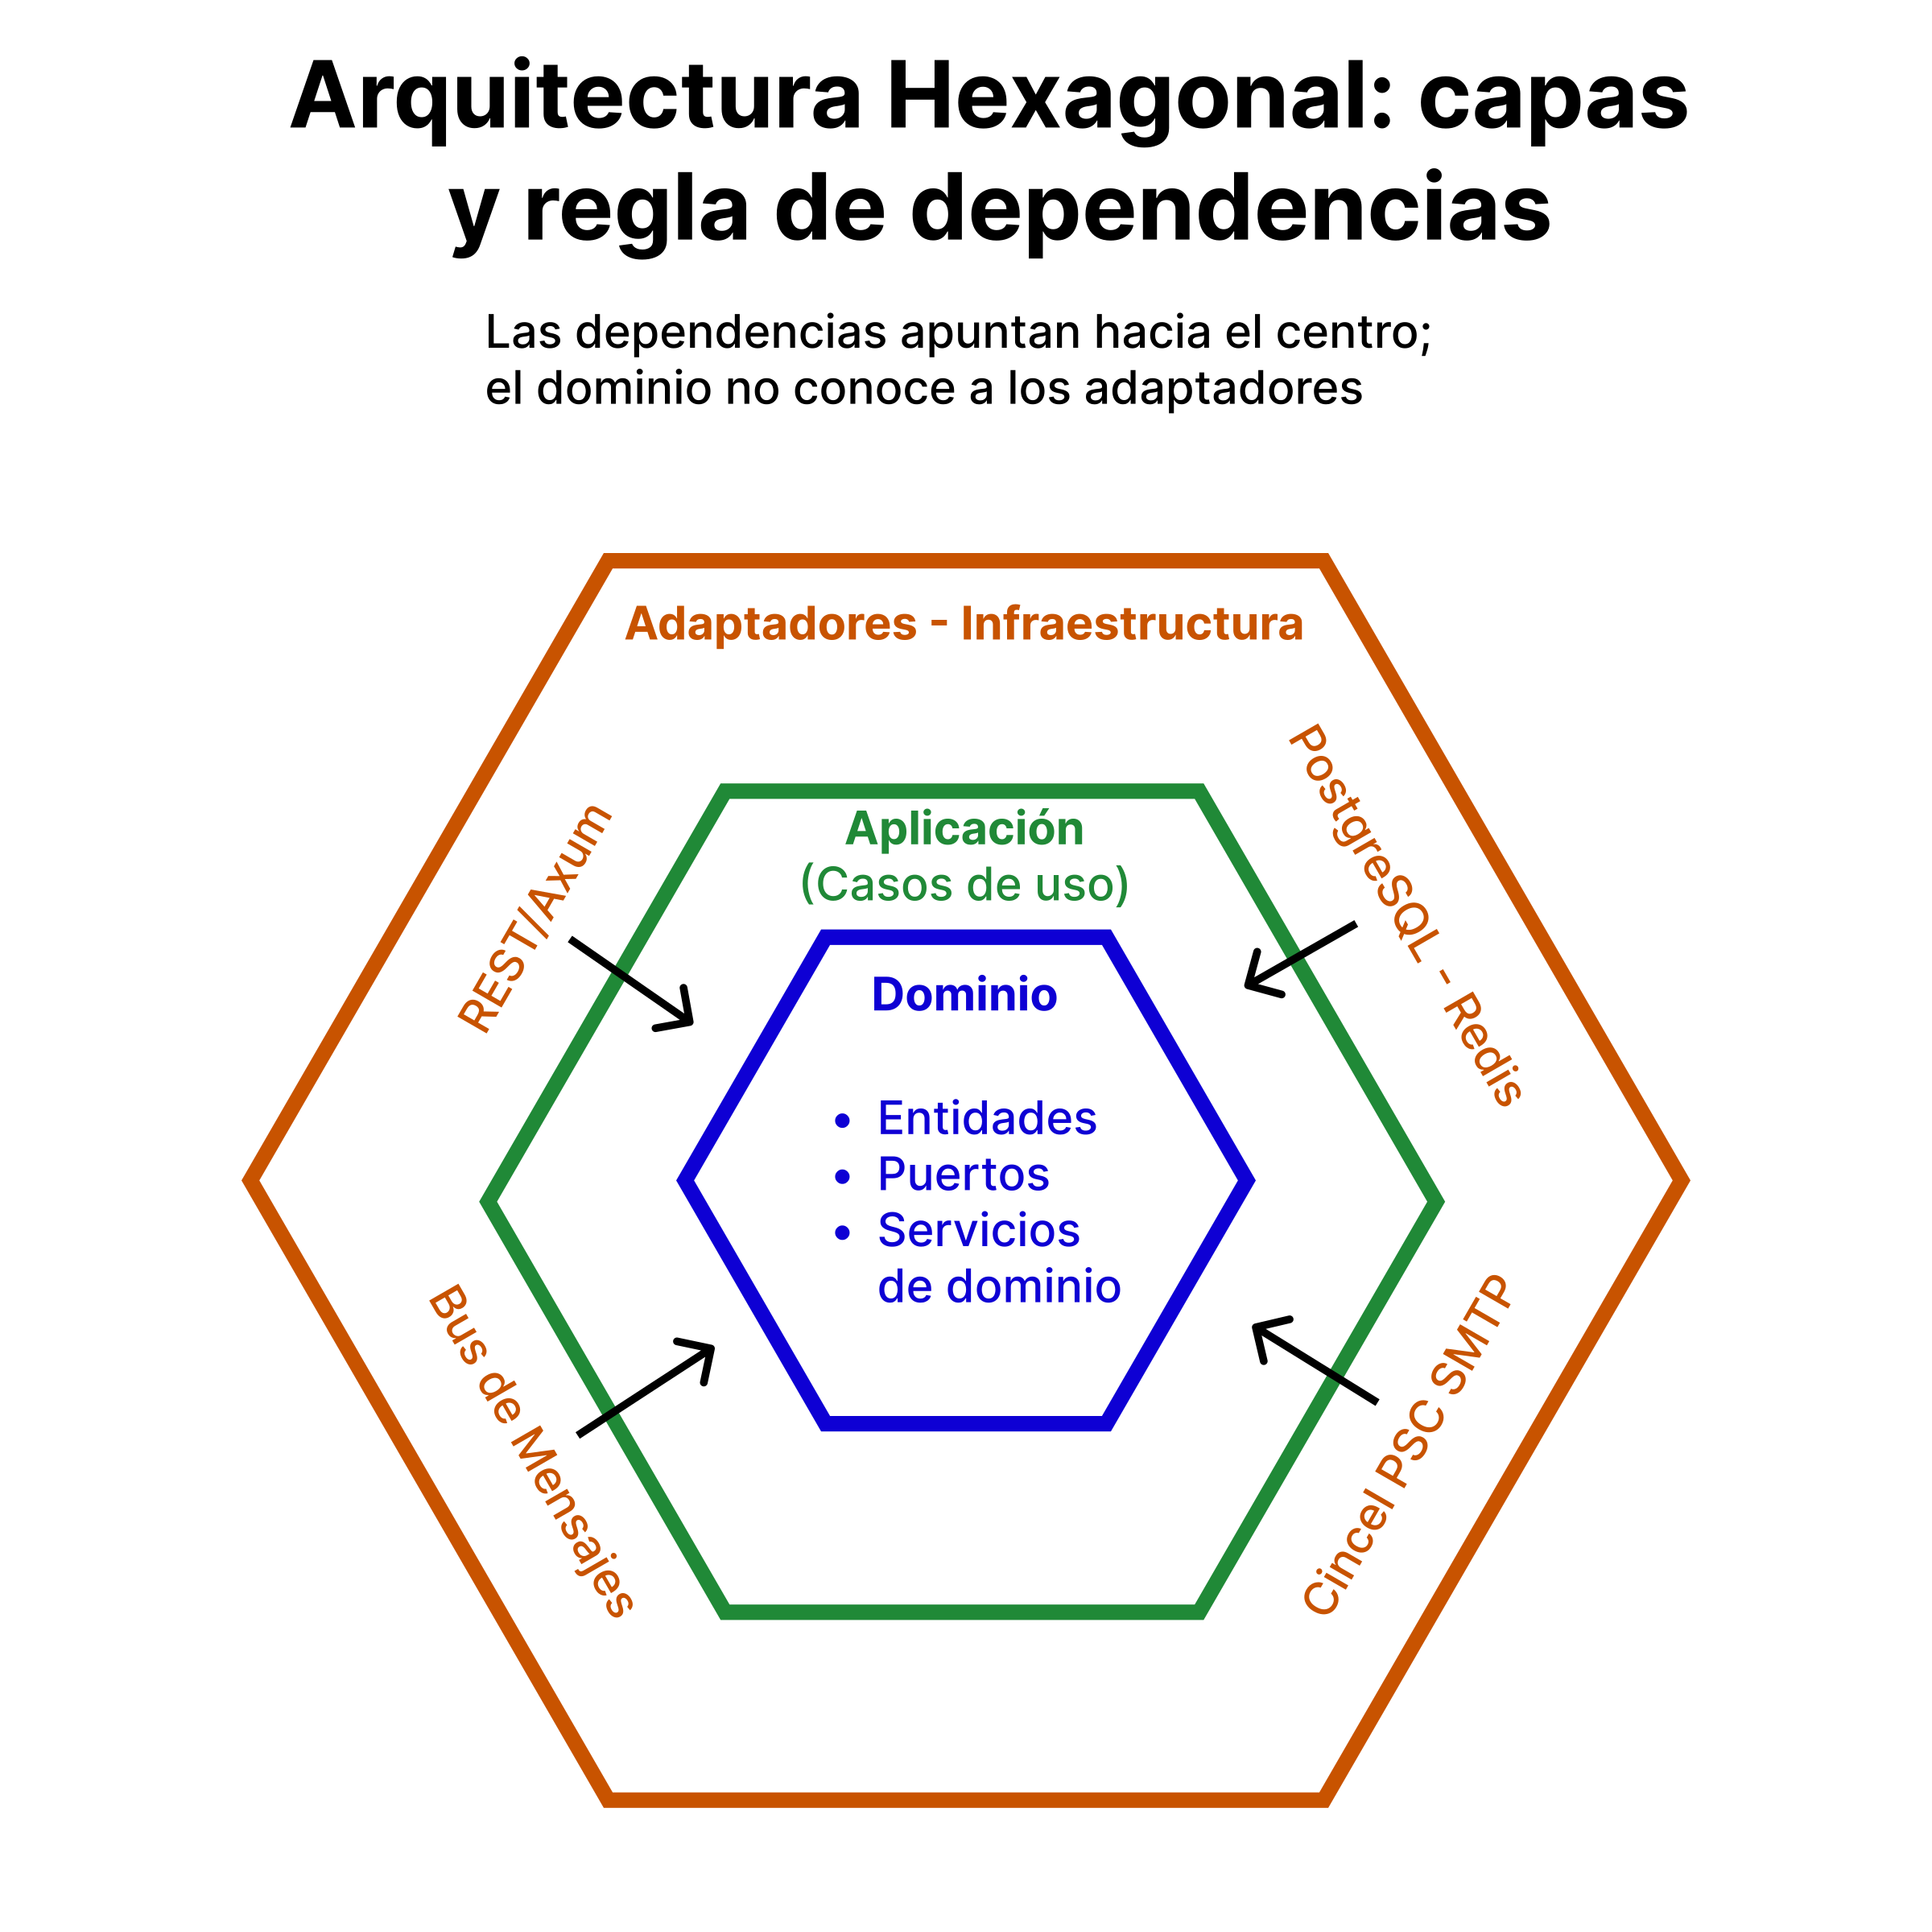
\includegraphics[width=0.82\linewidth]{image24.png}
  \caption{Arquitectura Hexagonal: capas conceptuales y regla de dependencias. Las dependencias siempre apuntan hacia el dominio.}
  \label{fig:hexagonal}
\end{figure}

El compilador de Rust verifica en tiempo de compilación que PostgresCaseRepository cumple con el contrato declarado por el trait CaseRepository. Cualquier divergencia (firma incorrecta, tipo de retorno incompatible, ausencia de un método requerido) impide la compilación del programa. Esta verificación mecánica elimina una categoría completa de errores que en lenguajes con tipado dinámico solo se manifestarían en tiempo de ejecución.

\subsection{Vista de Componentes y Bounded Contexts}\label{sec:vista-componentes}

La vista de componentes desciende un nivel respecto a la vista de contexto y muestra la organización interna del sistema en términos de bounded contexts —contextos limitados— derivados directamente de las siete agrupaciones funcionales declaradas en §3.2. El concepto de bounded context, introducido por Eric Evans en el contexto de Domain-Driven Design \cite{evans2003}, denota una zona del modelo dentro de la cual los conceptos del lenguaje ubicuo tienen un significado específico y consistente.

El sistema se descompone en siete bounded contexts: Identidad y Acceso (autenticación, RBAC, MFA), Gestión de Casos (expedientes y transiciones procesales), Calendario y Plazos (audiencias y plazos del CNPP), Documentos y Custodia (carga, clasificación y cadena de custodia), Servicios Criptográficos (firma, sellado y verificación), Firma de Contratos (firma con sellado de tiempo) y Operaciones y Auditoría (tableros de control, informes y bitácora). Servicios Criptográficos es un servicio compartido del que dependen tanto Documentos y Custodia como Firma de Contratos.

\begin{figure}[H]
  \centering
  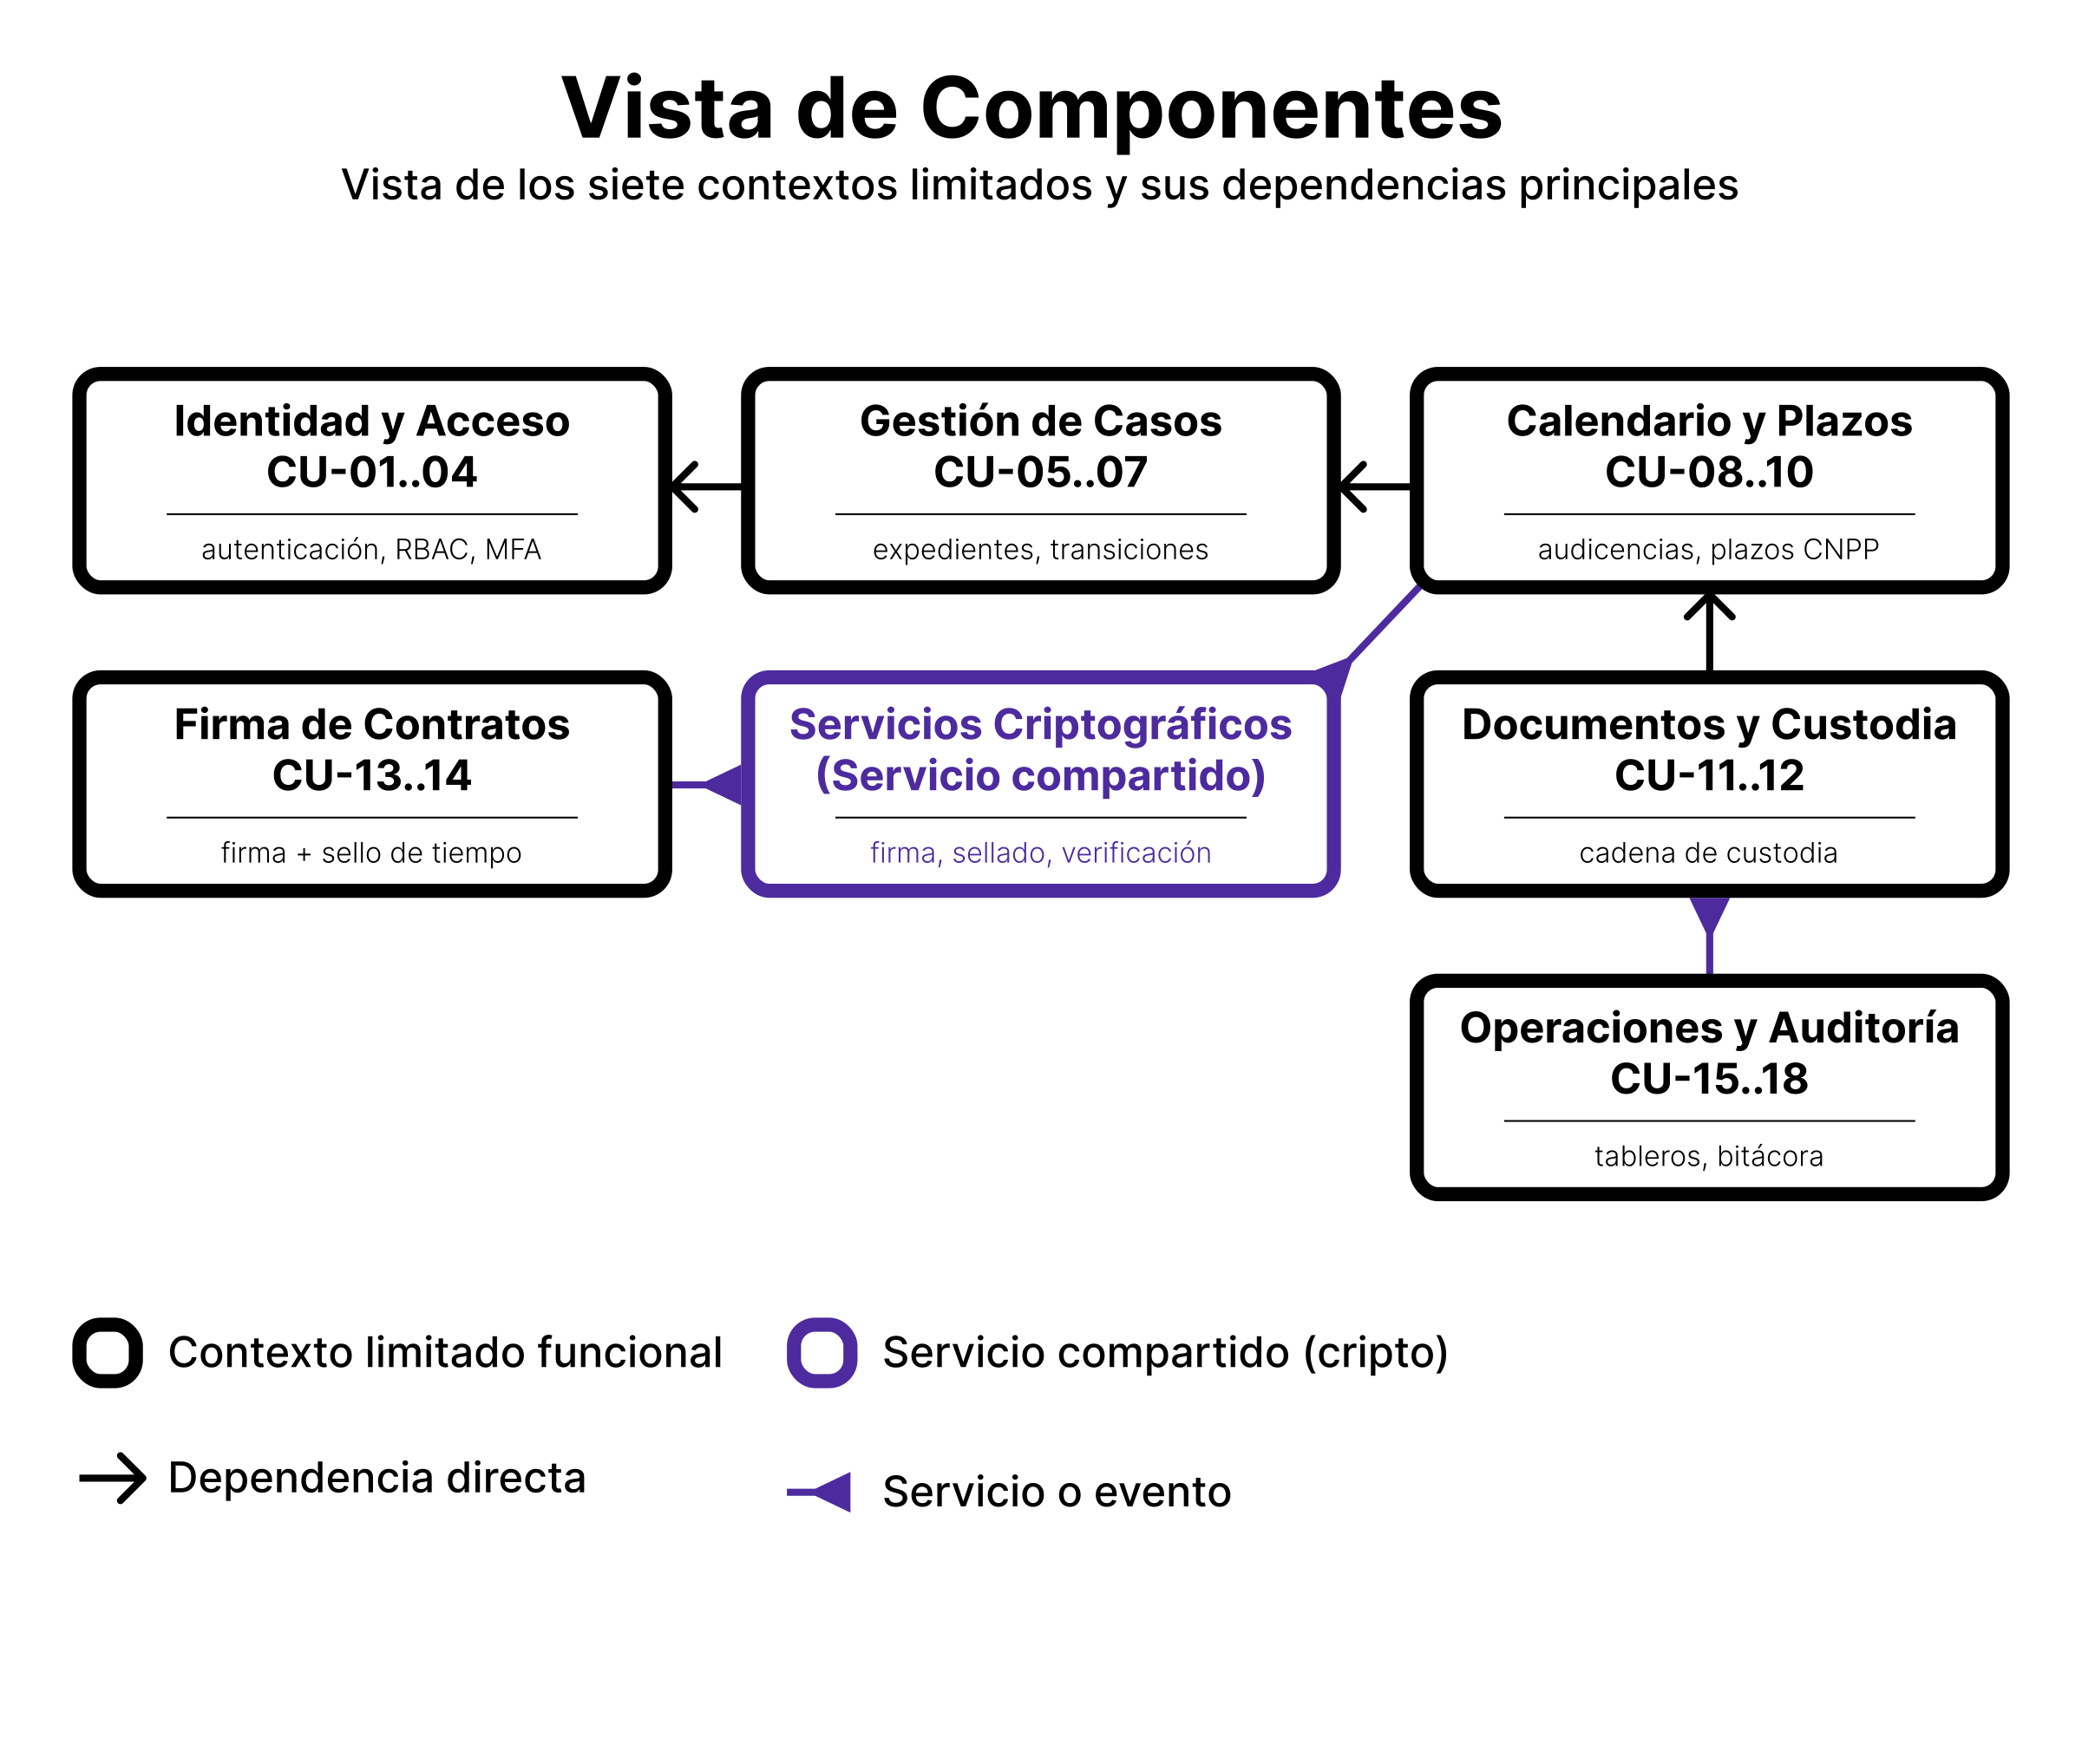
\includegraphics[width=0.9\linewidth]{image25.png}
  \caption{Vista de componentes: siete contextos limitados del sistema y sus dependencias principales.}
  \label{fig:componentes}
\end{figure}

El mapeo entre cada bounded context, los casos de uso que implementa y el crate del workspace de Cargo donde reside su código se presenta en la \cref{tab:bounded-contexts}. Esta correspondencia permite que las modificaciones a un bounded context queden contenidas dentro de un crate específico, facilitando la atribución de cambios y la asignación de responsabilidades.

\begin{table}[H]
  \centering
  \caption{Mapeo entre contextos delimitados, casos de uso y módulos del workspace de Cargo.}
  \label{tab:bounded-contexts}
  \begin{tabularx}{\linewidth}{@{}L{0.30\linewidth}C{0.18\linewidth}X@{}}
    \toprule
    \textbf{Contexto delimitado} & \textbf{Casos de uso} & \textbf{Crate / módulo} \\
    \midrule
    Identidad y Acceso & CU-01..04 & \texttt{domain::identity}, \texttt{application::identity} \\
    Gestión de Casos & CU-05..07 & \texttt{domain::case}, \texttt{application::case} \\
    Calendario y Plazos & CU-08..10 & \texttt{domain::calendar}, \texttt{application::calendar} \\
    Documentos y Custodia & CU-11..12 & \texttt{domain::document}, \texttt{application::document} \\
    Servicios Criptográficos & (transversal) & \texttt{domain::crypto}, \texttt{infrastructure::crypto} \\
    Firma de Contratos & CU-13..14 & \texttt{domain::contract}, \texttt{application::contract} \\
    Operaciones y Auditoría & CU-15..18 & \texttt{domain::audit}, \texttt{application::audit} \\
    \bottomrule
  \end{tabularx}
\end{table}

\subsection{Estructura del Workspace de Cargo}\label{sec:workspace-cargo}

El proyecto se organiza como un workspace de Cargo —el sistema de compilación y gestión de paquetes de Rust— compuesto por cinco crates miembros con responsabilidades estrictamente delimitadas y dependencias permitidas que enforce mecánicamente la regla de la arquitectura hexagonal. Esta estructura se documenta en el \texttt{Cargo.toml} raíz del proyecto y se valida en cada compilación.

Los cinco crates son: domain (entidades, value objects, traits/puertos y errores de dominio; sus únicas dependencias externas son serde, thiserror, time, uuid y zeroize), application (casos de uso, comandos y consultas; depende exclusivamente de domain y de async-trait), infrastructure (adaptadores driven que implementan los traits del dominio; depende de domain y application), web (adaptadores driving HTTP construidos con Axum, middleware Tower, DTOs y serialización HTTP; depende de application y domain), y bin (composition root que instancia los adaptadores concretos y los inyecta en los casos de uso; depende de todos los anteriores). La \cref{fig:workspace} representa esta estructura y las dependencias que el grafo de Cargo permite o prohíbe.

\begin{figure}[H]
  \centering
  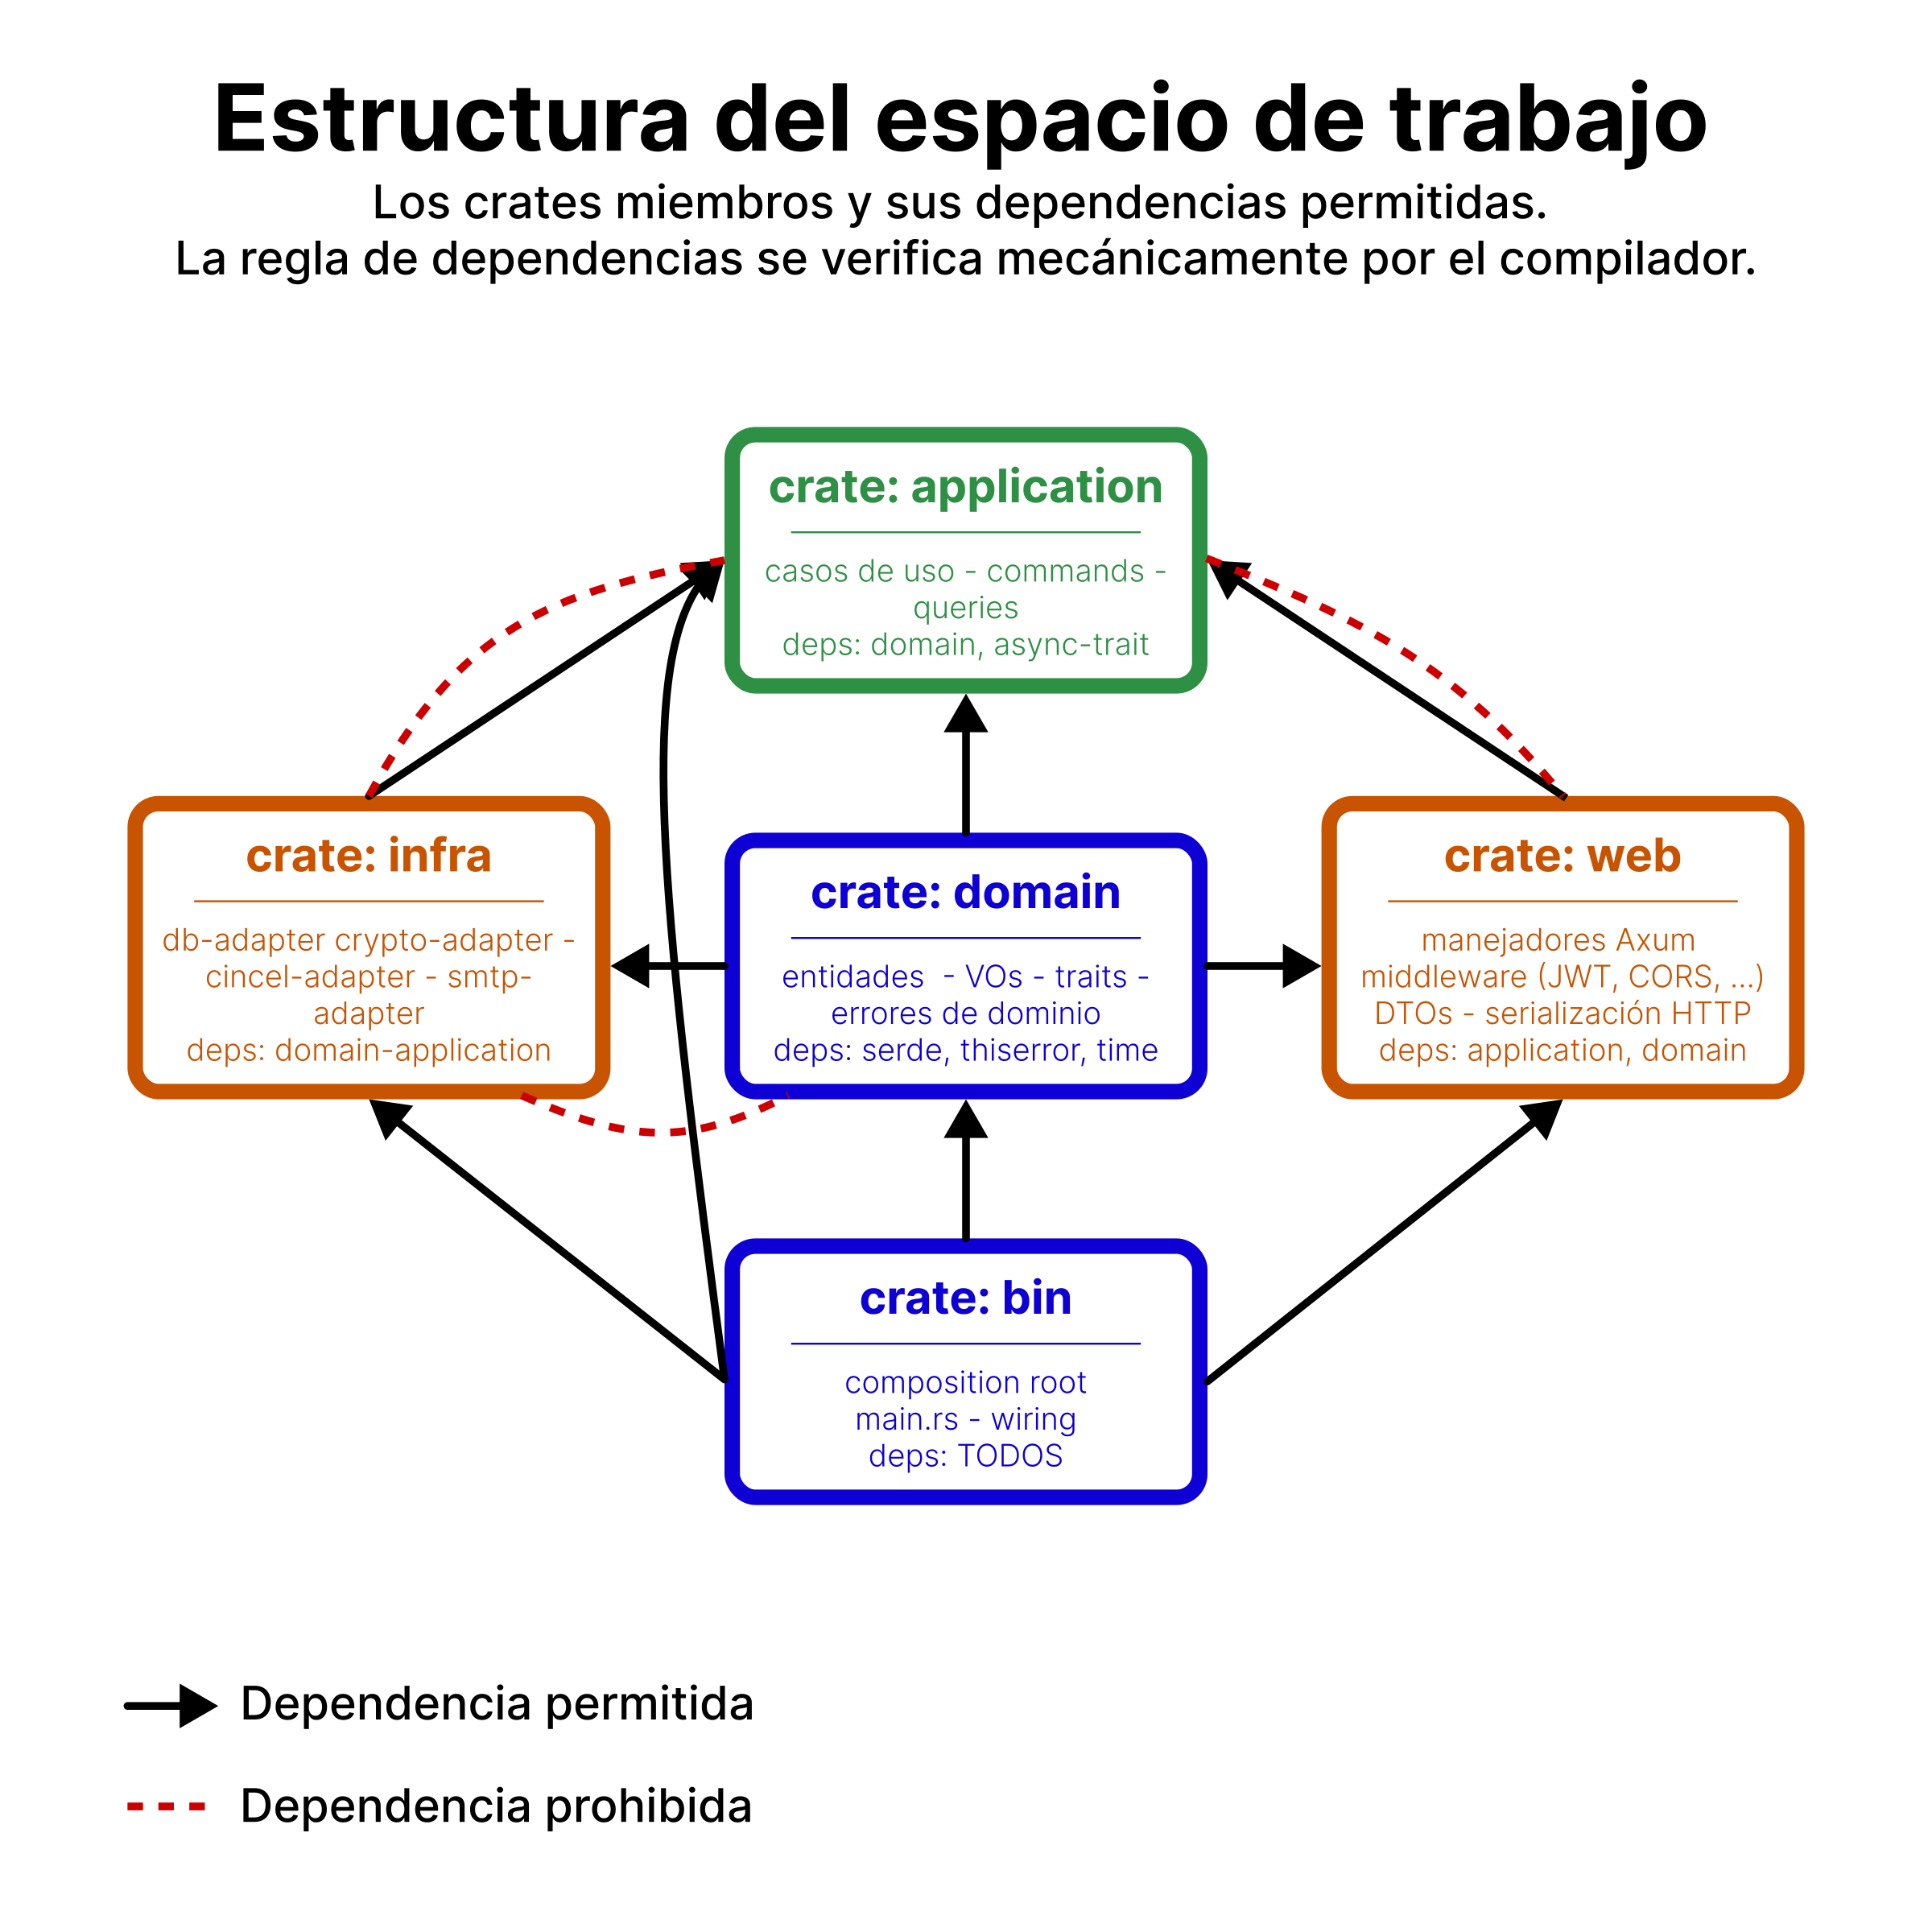
\includegraphics[width=0.9\linewidth]{image26.png}
  \caption{Estructura del workspace de Cargo: cinco crates miembros con dependencias permitidas (flechas negras) y prohibidas (flechas rojas punteadas).}
  \label{fig:workspace}
\end{figure}

La consecuencia técnica de esta organización es que las dependencias prohibidas no son una convención que el equipo deba recordar respetar: son una imposibilidad mecánica. Si un módulo del crate domain intenta importar un símbolo del crate infrastructure mediante una declaración \texttt{use infrastructure::PostgresCaseRepository}, el compilador emite el error «unresolved import» porque el \texttt{Cargo.toml} de domain no incluye infrastructure entre sus dependencias. La regla de dependencias se verifica mecánicamente por el compilador en cada build.

El sistema de Cargo features se utiliza para alternar adaptadores intercambiables en tiempo de compilación. Por ejemplo, la feature cincel-tsa activa el adaptador para el PSC Cincel, mientras que una futura feature seguridata-tsa activaría un adaptador alternativo para el PSC SeguriData. La selección se realiza al compilar el binario, manteniendo un único path de código para cada despliegue específico y evitando la complejidad de un sistema de inyección de dependencias en runtime.

\subsection{Stack Tecnológico}\label{sec:stack-tecnologico}

Esta subsección documenta y justifica las tecnologías concretas seleccionadas para implementar el sistema. Cada elección se sustenta en los atributos de calidad priorizados en §3.7.1 y se compara explícitamente con sus alternativas serias del ecosistema actual. Las decisiones más estructurantes se registran adicionalmente como ADRs formales en §3.7.10.

\subsubsection{Justificación de Rust como lenguaje del backend}\label{sec:rust-backend}

El backend del prototipo se implementa en Rust \cite{klabnik2023}. La selección responde principalmente a los atributos de seguridad e integridad priorizados en §3.7.1, en cuanto Rust elimina por construcción —mediante su sistema de ownership y verificación en tiempo de compilación— las clases de errores de memoria que han sido históricamente la fuente principal de vulnerabilidades explotables en software de sistemas. Microsoft ha documentado que aproximadamente el 70\% de las vulnerabilidades reportadas en sus productos a lo largo de una década correspondieron a errores de manejo de memoria \cite{msrc2019}; un porcentaje similar ha sido reportado por el equipo de seguridad de Chromium. Rust elimina categóricamente estos errores sin recurrir a un recolector de basura, lo que lo distingue de Go, Java o cualquier lenguaje con runtime managed.

Frente a Go, Rust ofrece tipos algebraicos (Result, Option, enums con datos asociados) que permiten modelar errores y casos especiales como parte del sistema de tipos, en lugar de mediante valores centinela o múltiples valores de retorno como hace Go. Esta expresividad es particularmente valiosa para un dominio en el que los errores deben ser explícitos y exhaustivos —una operación de firma puede fallar por certificado revocado, por reloj fuera de sincronía con la TSA, por documento que excede el tamaño máximo, entre otros casos—, y donde olvidar manejar uno de ellos no debe ser silencioso. Rust también ofrece zero-cost abstractions, permitiendo construir abstracciones de alto nivel (traits genéricos, iteradores) sin penalización en tiempo de ejecución, lo que Go renuncia a soportar por su modelo de simplicidad explícita.

Frente a Java o Kotlin con Spring, Rust evita el costo del runtime JVM —tiempo de arranque del orden de segundos, huella de memoria elevada, dependencia de un intérprete de bytecode— que es desproporcionado para un prototipo desarrollado en un equipo de desarrollo individual. Frente a Node.js con TypeScript, Rust proporciona tipado estático verificado en compilación (TypeScript es type erasure: los tipos desaparecen en runtime y no protegen contra errores reales del mundo) y rendimiento criptográfico sustancialmente superior, esencial para un sistema cuyo eje son las operaciones de firma, hash y cifrado intensivo. Frente a Python con FastAPI, Rust elimina el Global Interpreter Lock que limita la concurrencia real de Python, y ofrece un ecosistema criptográfico que ha sido sometido a auditorías formales independientes (particularmente la biblioteca ring, que utilizamos para las primitivas).

Una propiedad operacional adicional de Rust pertinente al alcance del prototipo es que el binario resultante es ejecutable único, sin dependencia de runtime, intérprete ni gestor de paquetes en producción. El despliegue se reduce a copiar un archivo de aproximadamente 15 MB al servidor objetivo, lo que simplifica la operación y reduce significativamente la superficie de ataque del entorno desplegado.

\subsubsection{Backend: Axum sobre el ecosistema tokio, tower y hyper}\label{sec:axum}

Como framework web se selecciona Axum, desarrollado por el equipo de tokio. Axum se construye sobre tres capas estándar de facto en el ecosistema Rust: tokio como runtime asíncrono multi-thread con scheduler work-stealing, tower como abstracción de middleware componible basada en el trait \texttt{Service<Request, Response>}, y hyper como implementación de los protocolos HTTP/1.1 y HTTP/2. Esta estratificación permite que cada nivel de la pila se evalúe y evolucione independientemente, y que los componentes desarrollados para tower puedan reutilizarse fuera del contexto HTTP.

Axum se distingue de alternativas como actix-web o rocket por no ser opinado respecto a la organización del código de la aplicación, lo que facilita la implementación del estilo arquitectónico hexagonal seleccionado en §3.7.3 sin tener que combatir las convenciones del framework. Los handlers de Axum reciben sus dependencias mediante extractores tipados (extractors), permitiendo inyectar los casos de uso de la capa de aplicación de manera explícita y verificable en compilación.

El pipeline de middleware Tower se configura para ejecutar, en orden, los siguientes interceptores transversales: CORS para el control de origen cruzado de peticiones del navegador; Rate Limiting con ventana deslizante para protección contra abuso; Tracing con propagación de identificador de petición para observabilidad; autenticación JWT para verificación de identidad del solicitante; logging estructurado para auditoría operativa. Cada middleware es composable —su ejecución se especifica declarativamente al construir el router— y verificable en compilación por el sistema de tipos.

\subsubsection{Frontend: Astro con Svelte Islands}\label{sec:frontend-astro}

El frontend del sistema se implementa con Astro como meta-framework y Svelte como librería de componentes interactivos, siguiendo el patrón Islands Architecture propuesto por Sylor-Miller y Miller \cite{sylormiller2019}. Bajo este patrón, las páginas se renderizan como HTML estático por defecto, y solo los componentes que requieren interactividad (calendario jurídico, dashboard, interfaz de verificación de firma) se hidratan selectivamente como islas reactivas. Esta estrategia minimiza el JavaScript enviado al navegador a aquello estrictamente necesario, mejorando los tiempos de carga y reduciendo la superficie de ataque del cliente.

Frente a Next.js con React, Astro y Svelte tienen tres ventajas específicas para el alcance del prototipo. Primero, Svelte compila a JavaScript imperativo sin Virtual DOM ni runtime de framework, produciendo bundles considerablemente más ligeros que React. Segundo, la reactividad de Svelte es sintáctica —se declara con \texttt{\$:} y asignaciones a variables— lo que reduce el boilerplate frente al modelo de hooks de React. Tercero, Astro está diseñado desde su concepción para emitir el mínimo JavaScript posible, mientras que Next.js parte del modelo de SPA hidratada completa y solo recientemente ha introducido los Server Components para mitigar ese problema.

Frente a SvelteKit puro, Astro se elige porque las páginas mayoritariamente informativas del sistema (landing, documentación, vistas de solo lectura) no se benefician de hidratación completa; ahí Astro emite HTML estático directamente. SvelteKit, en cambio, hidrata todas las páginas como SPA, perdiendo la oportunidad de servir contenido estático puro. La combinación Astro + Svelte aprovecha lo mejor de ambos: contenido estático por defecto y reactividad rica solo donde se necesita.

\subsubsection{Persistencia híbrida}\label{sec:persistencia-hibrida}

El sistema emplea un modelo de persistencia híbrido que combina PostgreSQL como base de datos relacional para los datos con valor probatorio, con Redis como almacén clave-valor en memoria para datos volátiles y comunicación en tiempo real. La justificación completa de esta separación, los esquemas de cada motor, y el mecanismo de encadenamiento criptográfico SHA-256 que garantiza la inmutabilidad de la bitácora de auditoría se documentan en §3.8 (Modelado de Base de Datos Híbrida). Los crates utilizados para acceder a cada motor son sqlx para PostgreSQL —que ofrece verificación de queries SQL en tiempo de compilación contra el esquema real— y fred para Redis —cliente asíncrono con soporte nativo para pub/sub.

\subsubsection{Inventario completo de crates}\label{sec:inventario-crates}

El proyecto utiliza un conjunto curado de crates externos del ecosistema Rust, todos publicados en crates.io con versiones pinneadas en los archivos \texttt{Cargo.toml} de cada crate del workspace. Los crates se agrupan por capa arquitectónica para facilitar la auditoría y para enforce las reglas de dependencias entre capas discutidas en §3.7.6. La \cref{tab:inventario-crates} enumera los crates principales del proyecto, agrupados por capa y con sus respectivas funciones. La versión mínima soportada del compilador (Minimum Supported Rust Version, MSRV) es Rust 1.78 estable.

\begin{longtable}{@{}L{0.22\linewidth}L{0.22\linewidth}L{0.46\linewidth}@{}}
  \caption{Inventario de crates externos utilizados por el proyecto, agrupados por capa arquitectónica.}
  \label{tab:inventario-crates} \\
  \toprule
  \textbf{Capa} & \textbf{Crate} & \textbf{Función} \\
  \midrule
  \endfirsthead
  \toprule
  \textbf{Capa} & \textbf{Crate} & \textbf{Función} \\
  \midrule
  \endhead
  \midrule
  \multicolumn{3}{r@{}}{\emph{Continúa en la página siguiente}} \\
  \endfoot
  \bottomrule
  \endlastfoot
  Dominio & serde & Serialización/deserialización tipada \\
  Dominio & thiserror & Errores tipados por capa \\
  Dominio & time & Manejo de fechas con zona horaria \\
  Dominio & uuid & Identificadores únicos universales \\
  Dominio & zeroize & Borrado de material secreto en memoria al liberar (higiene de memoria) \\
  Aplicación & async-trait & Traits asíncronos \\
  Infraestructura cripto & ring & Hash, AES-GCM, HMAC (auditado) \\
  Infraestructura cripto & x509-cert + der & Manejo de certificados X.509 RFC 5280 \\
  Infraestructura cripto & rsa & Firma digital RSA-3072 PKCS\#1 v1.5 \\
  Infraestructura cripto & argon2 & Hashing de contraseñas (RFC 9106) \\
  Infraestructura cripto & totp-rs & Autenticación multifactor TOTP (RFC 6238) \\
  Infraestructura cripto & cms + x509-tsp & Parseo del token de sellado de tiempo RFC 3161 (CMS SignedData y TSTInfo) \\
  Infraestructura datos & sqlx & Cliente PostgreSQL con verificación en compile-time \\
  Infraestructura datos & fred & Cliente Redis asíncrono con pub/sub \\
  Infraestructura datos & fs2 & Bloqueo advisory de archivos compartidos entre procesos \\
  Infraestructura red & reqwest & Cliente HTTP asíncrono (Cincel TSA) \\
  Infraestructura red & lettre & Cliente SMTP con TLS y SASL \\
  Web/HTTP & axum & Framework web sobre tokio/tower/hyper \\
  Web/HTTP & tower / tower-http & Middleware composable \\
  Web/HTTP & tokio & Runtime asíncrono multi-thread \\
  Interfaz de línea de comandos & clap & Análisis declarativo de argumentos y subcomandos \\
  Observabilidad & tracing + tracing-subscriber & Logs estructurados con spans \\
  Validación & validator & Validación de DTOs HTTP \\
  Configuración & config + dotenvy & Carga de configuración desde entorno \\
  Errores (boundaries) & anyhow & Errores polimórficos en \texttt{main.rs} y tests \\
  Testing & mockall, proptest, rstest, wiremock & Mocks, pruebas basadas en propiedades, fixtures, mock HTTP \\
\end{longtable}

\subsection{Patrones Arquitectónicos Transversales}\label{sec:patrones-transversales}

Esta subsección documenta cuatro patrones que atraviesan transversalmente todas las capas de la arquitectura. Su tratamiento explícito y consistente es lo que permite que el sistema mantenga coherencia operativa en escala: errores tipados, concurrencia estructurada, inyección de dependencias por composición, y observabilidad estructurada.

\subsubsection{Manejo de errores}\label{sec:manejo-errores}

El sistema adopta una estrategia de errores tipados por capa, implementada con la macro derive de thiserror. Cada capa define su propio tipo de error con variantes específicas: DomainError captura las violaciones de invariantes de negocio (caso inválido, transición prohibida, firma rechazada); ApplicationError envuelve errores de orquestación de casos de uso e incluye DomainError como variante; los crates de infraestructura definen errores específicos de su backend (PostgresError, CincelError, SmtpError); finalmente, ApiError representa errores HTTP y mapea desde las capas anteriores mediante el trait IntoResponse de Axum.

Esta tipificación contrasta con el uso indiscriminado de anyhow, que se reserva exclusivamente para el binario principal (\texttt{bin/main.rs}) y para las pruebas, donde la conveniencia del polimorfismo de errores supera la necesidad de discriminar tipos. En cambio, en los crates de dominio, aplicación e infraestructura, los errores deben ser exhaustivos y discriminables porque cada caller necesita decidir qué hacer ante cada variante específica.

\subsubsection{Modelo de concurrencia asíncrona}\label{sec:concurrencia-asincrona}

El sistema utiliza tokio como runtime asíncrono multi-thread con scheduler work-stealing, configurado por defecto con tantos worker threads como núcleos lógicos disponibles. Las operaciones I/O bound (consultas a PostgreSQL, llamadas a Cincel, envíos SMTP) se ejecutan asíncronamente sin bloquear los workers, permitiendo concurrencia masiva con un consumo modesto de threads del sistema operativo. La concurrencia entre tareas se estructura mediante \texttt{tokio::spawn} con joins explícitos —siguiendo el principio de structured concurrency— para garantizar que ninguna tarea escape del scope de su parent y produzca leaks o panics no manejados.

Las operaciones que pueden quedar bloqueadas indefinidamente (invocaciones HTTP a sistemas externos, esperas a locks distribuidos) se envuelven con \texttt{tokio::time::timeout} para garantizar terminación acotada. Las operaciones cancelables utilizan CancellationToken propagado desde el handler raíz, permitiendo que un cliente que cierra la conexión HTTP libere inmediatamente todos los recursos asociados a su petición. Los traits Send + Sync requeridos para los puertos garantizan en tiempo de compilación que cualquier implementación es segura para usar entre threads, eliminando una categoría completa de errores de concurrencia.

\subsubsection{Inyección de dependencias por composición}\label{sec:inyeccion-dependencias}

La inyección de dependencias se realiza por composición explícita en el composition root —el archivo \texttt{bin/main.rs}—, sin recurrir a un contenedor de DI en runtime. Los casos de uso reciben sus dependencias como parámetros genéricos restringidos por traits (\texttt{impl Trait}) o como trait objects (\texttt{Arc<dyn Trait>}). Por ejemplo, el caso de uso SignContract se define como \texttt{SignContract<R, S, T>} donde R: CaseRepository, S: DocumentSigner, T: TimestampService; \texttt{main.rs} construye PostgresCaseRepository, RsaPkcs1Signer y CincelTsaAdapter, los inyecta en SignContract, y registra el resultado en el router de Axum. Esta estrategia es completamente verificable en tiempo de compilación —si un adaptador no satisface el contrato del puerto, el programa no compila— y elimina la categoría de errores característicos de los frameworks DI (dependencias no resueltas, ciclos detectados solo en runtime, configuraciones mal escritas).

\subsubsection{Observabilidad estructurada}\label{sec:observabilidad}

El sistema utiliza el ecosistema tracing para producir logs estructurados con spans tipados. Cada petición HTTP genera un span raíz con un \texttt{request\_id} propagado a través de todas las invocaciones asíncronas mediante el contexto de tokio. Los logs se emiten en formato JSON line-delimited (JSONL), facilitando su ingesta por agregadores como Vector, Loki o Elasticsearch. Los niveles de verbosidad son configurables por módulo a través de la variable de entorno \texttt{RUST\_LOG}, permitiendo aumentar temporalmente el detalle de una capa específica sin reiniciar el servicio. Para trazabilidad distribuida, el crate tracing-opentelemetry permite exportar spans a backends compatibles (Jaeger, Tempo) sin modificar el código de la aplicación. La política de redacción de información sensible (referencia cruzada a RNF-03) está implementada como un layer personalizado del subscriber, que aplica patrones regex sobre los campos antes de su emisión para sanitizar secretos y material criptográfico que pudieran filtrarse.

\subsection{Vista de Seguridad: Fronteras de Confianza}\label{sec:vista-seguridad}

Esta subsección desarrolla la vista de seguridad arquitectónica, complementaria al diseño criptográfico detallado en §3.11. Mientras §3.11 documenta los algoritmos criptográficos específicos (RSA-3072, AES-256-GCM, SHA-256, RFC 3161, PKI con CA interna) y sus parámetros, esta subsección documenta cómo esos mecanismos se distribuyen entre las distintas zonas de confianza del sistema y qué controles se aplican en cada cruce de frontera.

El modelo adoptado sigue el principio de defensa en profundidad formalizado por Saltzer y Schroeder \cite{saltzer1975} y desarrollado operativamente en el OWASP Application Security Verification Standard \cite{owasp2021}. La Figura A.1 en el Anexo A presenta el modelo completo con cuatro zonas de confianza y los controles de seguridad aplicados en cada cruce.

El sistema se modela como cuatro zonas de confianza separadas por tres fronteras explícitas. La primera zona, la red pública, comprende todo aquello que no está bajo control directo del sistema: el navegador del usuario final, los actores adversarios potenciales, y los servicios externos como Cincel PSC y los proveedores SMTP que aunque sean legítimos no operan dentro del perímetro de seguridad del prototipo. La segunda zona, el perímetro de aplicación, contiene el reverse proxy con terminación TLS y la API pública expuesta. La tercera zona, el núcleo aplicativo, contiene el binario Rust con sus tres módulos internos (web, application, domain). La cuarta y más confiable zona, datos persistentes y secretos, contiene PostgreSQL, Redis y el subsistema de gestión de claves criptográficas.

El cruce de la primera frontera —de la red pública al perímetro de aplicación— se controla mediante terminación TLS 1.3 con suites de cifrado modernas; rate limiting con ventana deslizante para protección contra abuso de la API; un Web Application Firewall que filtra patrones de ataque conocidos; y cabeceras CORS estrictas que restringen el origen de las peticiones legítimas. La superficie expuesta a esta frontera es deliberadamente mínima: solo los endpoints HTTPS estrictamente necesarios.

El cruce de la segunda frontera —del perímetro al núcleo aplicativo— se controla mediante autenticación basada en JWT (JSON Web Token) firmado por la propia aplicación; validación exhaustiva de toda entrada del usuario antes de cualquier procesamiento; y autorización basada en roles (RBAC) que restringe qué operaciones puede invocar cada rol (socio, paralegal, cliente). Cualquier petición que no satisfaga las tres verificaciones es rechazada con un código de error apropiado y registrada en la bitácora de auditoría.

El cruce de la tercera frontera —del núcleo aplicativo a datos persistentes y secretos— se controla mediante conexiones TLS internas entre el binario Rust y los motores de PostgreSQL y Redis; uso obligatorio de consultas parametrizadas mediante sqlx (que verifica en compile-time la conformidad de cada query con el esquema, eliminando la posibilidad de inyección SQL); y cifrado en reposo de todos los documentos mediante el patrón envelope encryption con KEK protegida por el módulo de gestión de claves (cuyo diseño detallado se documenta en §3.11.4).

Los servicios externos se modelan como entidades de la zona no confiable a las que el sistema invoca explícitamente con canales seguros: un PSC externo futuro para sellado de tiempo (RFC 3161) utilizará TLS y verificación de la firma del sello recibido; la TSA local de demostración opera sin salir del perímetro del prototipo; la integración con el proveedor SMTP utiliza TLS más autenticación SASL. En ningún caso se confía en estos servicios para operaciones de seguridad sin verificación local del resultado: un sello recibido se verifica criptográficamente contra la cadena de certificados del emisor antes de ser aceptado e incorporado al expediente.

El modelo de amenazas STRIDE de Shostack \cite{shostack2014} se aplicó como herramienta de revisión sistemática durante el diseño para verificar que cada una de las seis categorías de amenazas (Spoofing, Tampering, Repudiation, Information Disclosure, Denial of Service, Elevation of Privilege) tuviese al menos un control asignado. La matriz resultante demuestra que la combinación de los controles enumerados ofrece cobertura para todas las categorías, con énfasis particular en Tampering (mediante el encadenamiento SHA-256 de la bitácora) y Repudiation (mediante el sellado de tiempo independiente del PSC).

\subsection{Decisiones Arquitectónicas Significativas (ADRs)}\label{sec:adrs}

Las decisiones arquitectónicas más estructurantes del sistema se registran formalmente como Architecture Decision Records (ADRs) en el formato propuesto por Michael Nygard \cite{nygard2011}. Cada ADR documenta de forma autocontenida cuatro elementos: el contexto del problema que motivó la decisión, las alternativas consideradas, la decisión adoptada, y las consecuencias —tanto positivas como negativas— de la decisión. Los seis ADRs siguientes cubren las decisiones cuya reversión implicaría una refactorización significativa.

\subsubsection{ADR-01. Adopción de Arquitectura Hexagonal}\label{sec:adr-01}

Contexto: el sistema requiere alta testabilidad (XP/TDD) y evolvabilidad (sustitución de PSC, motor de BD). Alternativas: N-tier, Clean, Onion, Hexagonal, Microservicios, Monolito Modular sin patrón hexagonal. Decisión: Monolito Modular con Arquitectura Hexagonal de Cockburn. Consecuencias positivas: dominio aislado y testeable, adaptadores intercambiables, regla de dependencias verificable mecánicamente. Consecuencias negativas: ligero overhead de indirección por cada operación que cruza una capa, requiere disciplina del equipo para no introducir atajos.

\subsubsection{ADR-02. Rust como lenguaje del backend}\label{sec:adr-02}

Contexto: prototipo de seguridad con operaciones criptográficas intensivas. Alternativas: Go, Java/Kotlin con Spring, Node.js con TypeScript, Python con FastAPI. Decisión: Rust. Consecuencias positivas: seguridad de memoria sin GC, sistema de tipos algebraicos, ecosistema criptográfico auditado, binario único sin runtime. Consecuencias negativas: curva de aprendizaje del ownership y borrow checker, ecosistema más pequeño que Java o Node, tiempos de compilación más largos.

\subsubsection{ADR-03. Axum como framework web}\label{sec:adr-03}

Contexto: necesidad de un framework HTTP que no impusiera estructura incompatible con el estilo hexagonal. Alternativas: actix-web, rocket, warp. Decisión: Axum sobre tokio/tower/hyper. Consecuencias positivas: framework no opinado, ecosistema tower reutilizable para otros servicios, mantenido por el equipo de tokio. Consecuencias negativas: API ergonómica menos madura que actix-web, documentación todavía en evolución.

\subsubsection{ADR-04. Astro + Svelte Islands para el frontend}\label{sec:adr-04}

Contexto: páginas mayoritariamente informativas con islas de interactividad rica (calendario, dashboard, verificación de firma). Alternativas: Next.js + React, SvelteKit puro, Remix. Decisión: Astro como meta-framework con Svelte como librería de componentes interactivos. Consecuencias positivas: HTML estático por defecto, JavaScript mínimo enviado al cliente, Svelte sin Virtual DOM. Consecuencias negativas: dos sistemas de templating (Astro y Svelte) que el desarrollador debe conocer, ecosistema de componentes Svelte más pequeño que React.

\subsubsection{ADR-05. Monolito Modular sobre Microservicios}\label{sec:adr-05}

Contexto: equipo de desarrollo de dos personas en periodo académico, alcance del prototipo no requiere despliegue distribuido. Alternativas: descomposición en microservicios desde el inicio, monolito modular. Decisión: Monolito Modular siguiendo la recomendación MonolithFirst de Fowler \cite{fowler2015}. Consecuencias positivas: simplicidad operativa, despliegue como binario único, sin overhead de comunicación inter-servicios, facilidad de refactorización. Consecuencias negativas: escalado monolítico (ya aceptable para el alcance del prototipo), imposibilidad de desplegar componentes independientemente.

\subsubsection{ADR-06. Persistencia híbrida PostgreSQL + Redis}\label{sec:adr-06}

Contexto: el sistema maneja tanto datos con valor probatorio (que requieren persistencia transaccional duradera) como datos volátiles para sesiones, caché y notificaciones en tiempo real. Alternativas: PostgreSQL exclusivamente, Redis exclusivamente, PostgreSQL + Redis. Decisión: PostgreSQL para datos persistentes con responsabilidades específicas en §3.8.1, Redis para datos volátiles con TTL conforme a §3.8.2. Consecuencias positivas: cada motor utilizado para lo que mejor hace, baja latencia para sesiones y notificaciones, integridad transaccional para operaciones críticas. Consecuencias negativas: necesidad de operar dos motores de almacenamiento, mayor complejidad operativa, necesidad de coherencia eventual entre ambos.

\subsection{Trazabilidad Arquitectura ↔ Requerimientos}\label{sec:trazabilidad}

Esta subsección presenta la matriz de trazabilidad que cierra el Capítulo 3 demostrando que cada requerimiento funcional y no funcional cuenta con un componente arquitectónico responsable, y que ningún componente arquitectónico carece de justificación en un requerimiento. La \cref{tab:trazabilidad} sintetiza este mapeo en una vista de alto nivel; la matriz completa, con los diecisiete casos de uso (CU-01 a CU-17) y los catorce requerimientos no funcionales (RNF-01 a RNF-14 de §3.4), se entrega como anexo electrónico complementario al documento.

\begin{table}[H]
  \centering
  \caption{Mapeo de alto nivel entre componentes arquitectónicos y los requerimientos que satisfacen.}
  \label{tab:trazabilidad}
  \begin{tabularx}{\linewidth}{@{}L{0.42\linewidth}X@{}}
    \toprule
    \textbf{Componente arquitectónico} & \textbf{Requerimientos atendidos} \\
    \midrule
    Bounded Context «Identidad y Acceso» & CU-01..04, RNF-01, RNF-02 \\
    Bounded Context «Gestión de Casos» & CU-05..07, RNF-04 (parcial) \\
    Bounded Context «Calendario y Plazos» & CU-08..10 \\
    Bounded Context «Documentos y Custodia» & CU-11..12, RNF-03, RNF-04 \\
    Bounded Context «Servicios Criptográficos» & CU-11..14, RNF-03 \\
    Bounded Context «Firma de Contratos» & CU-13..14 \\
    Bounded Context «Operaciones y Auditoría» & CU-15..17, RNF-04, RF-20 \\
    Crate \texttt{domain} con traits (puertos) & Soporta evolvabilidad transversal \\
    Workspace de Cargo con regla de dependencias & Mantenibilidad transversal \\
    Pipeline Tower middleware & RF-01 (autenticación y sesiones), seguridad cross-cutting \\
    Modelo de fronteras de confianza (§3.7.9) & RNF-01, RNF-02, RNF-03 \\
    Subsistema observabilidad (tracing) & RF-20 (bitácora de actividad) \\
    \bottomrule
  \end{tabularx}
\end{table}

\subsubsection{Fitness functions}\label{sec:fitness-functions}

Siguiendo el enfoque de arquitecturas evolutivas formalizado por Ford, Parsons y Kua \cite{ford2023}, la coherencia entre la arquitectura prescrita y la arquitectura efectiva del código se verifica mediante un conjunto de fitness functions: pruebas automatizadas que comprueban propiedades arquitectónicas que no podrían verificarse mediante pruebas funcionales tradicionales. Estas fitness functions se ejecutan como parte del pipeline de Integración Continua y, en caso de fallo, bloquean la integración del cambio en la rama principal.

Las fitness functions implementadas para el prototipo son: (1) verificación de que ningún módulo del crate domain importa símbolos de los crates infrastructure ni web (verificada por el compilador en cada build); (2) verificación de que todo handler HTTP envuelve su lógica en un span de tracing (verificada con un lint personalizado de clippy); (3) verificación de que ningún log emitido contiene literales que matcheen patrones de claves criptográficas (verificada con un test que ejecuta toda la suite e inspecciona los logs producidos); (4) verificación de que cada trait que define un puerto driven tiene al menos una implementación concreta y al menos un mock para tests (verificada por inspección del workspace en cada build); (5) verificación de que el binario compilado no excede 25 MB (verificada por el pipeline de release).


\section{Modelado de Base de Datos Híbrida}\label{sec:bd-hibrida}

El sistema emplea un modelo de persistencia híbrido que combina \textbf{PostgreSQL} (base de datos relacional) con \textbf{Redis} (almacén clave-valor en memoria), con responsabilidades estrictamente delimitadas. Esta decisión responde a los requisitos funcionales y no funcionales identificados en el protocolo, particularmente RF-20 (bitácora de actividad), RNF-04 (integridad append-only) y la necesidad de notificaciones en tiempo real.

\subsection{PostgreSQL: Datos Persistentes con Valor Probatorio}\label{sec:postgresql}

PostgreSQL se selecciona como motor relacional principal por las siguientes razones: (1) soporte nativo de \textbf{JSONB} para metadatos variables de expedientes, lo que permite modelar la diversidad del sistema acusatorio oral mexicano (CNPP, Art. 211-215) sin sacrificar la integridad referencial; (2) \textbf{RULE} para enforce de append-only en la bitácora de auditoría, impidiendo operaciones UPDATE y DELETE a nivel de motor; (3) extensiones criptográficas nativas (pgcrypto); (4) tipo de dato INET para registro de direcciones IP en la bitácora.

La bitácora de auditoría (audit\_log) implementa un mecanismo de \textbf{encadenamiento SHA-256}: cada registro incluye un campo sha256\_chain calculado como el hash SHA-256 (véase §2.3.1) del valor sha256\_chain del registro anterior concatenado con los datos del registro actual, es decir, $\mathrm{sha256\_chain}(n) = \mathrm{SHA\text{-}256}(\mathrm{sha256\_chain}(n-1) \,\|\, \mathrm{registro}(n))$. Esto crea una cadena verificable de integridad que permite detectar cualquier manipulación retroactiva, cumpliendo con el Art. 33 del Código de Comercio (retención mínima de 10 años).

\subsubsection{Decisión de diseño: Single-Tenant}

El sistema se diseña para un solo despacho legal (single-tenant), eliminando la complejidad de aislamiento multi-tenant contemplada en el protocolo original (cuyos requerimientos se reformulan en RNF-01 y RNF-05 como aislamiento y privacidad de la información del despacho dentro de su instancia). Esta simplificación es coherente con el alcance del prototipo y reduce significativamente la superficie de ataque.

\subsection{Redis: Datos Volátiles y Comunicación en Tiempo Real}\label{sec:redis}

Redis se emplea exclusivamente para datos efímeros que \textbf{no requieren persistencia a largo plazo ni tienen valor probatorio}:

\begin{itemize}
  \item \textbf{Sesiones JWT}: almacenamiento de tokens de sesión con TTL configurable (24h por defecto), permitiendo invalidación inmediata por revocación.
  \item \textbf{Caché de permisos}: materialización temporal de las autorizaciones del usuario (TTL 5 minutos) para evitar consultas repetidas a PostgreSQL en cada petición.
  \item \textbf{Pub/Sub para notificaciones}: canal de comunicación entre el backend y los clientes WebSocket. Cuando ocurre un evento relevante (nuevo documento, firma completada, deadline próximo), se publica en un canal Redis que el adaptador WebSocket consume y retransmite al navegador del usuario.
  \item \textbf{Rate limiting}: contadores con ventana deslizante para protección contra abuso de la API.
  \item \textbf{Tokens temporales}: tokens de un solo uso para restablecimiento de contraseña y verificación MFA (TTL 15 minutos).
\end{itemize}

\subsection{Diagrama del Modelo de Datos}\label{sec:diagrama-datos}

La \cref{fig:modelo-datos} presenta el modelo de datos completo, mostrando las tablas de PostgreSQL (izquierda) con sus relaciones y las estructuras de Redis (derecha) con sus políticas de TTL.

\begin{figure}[H]
  \centering
  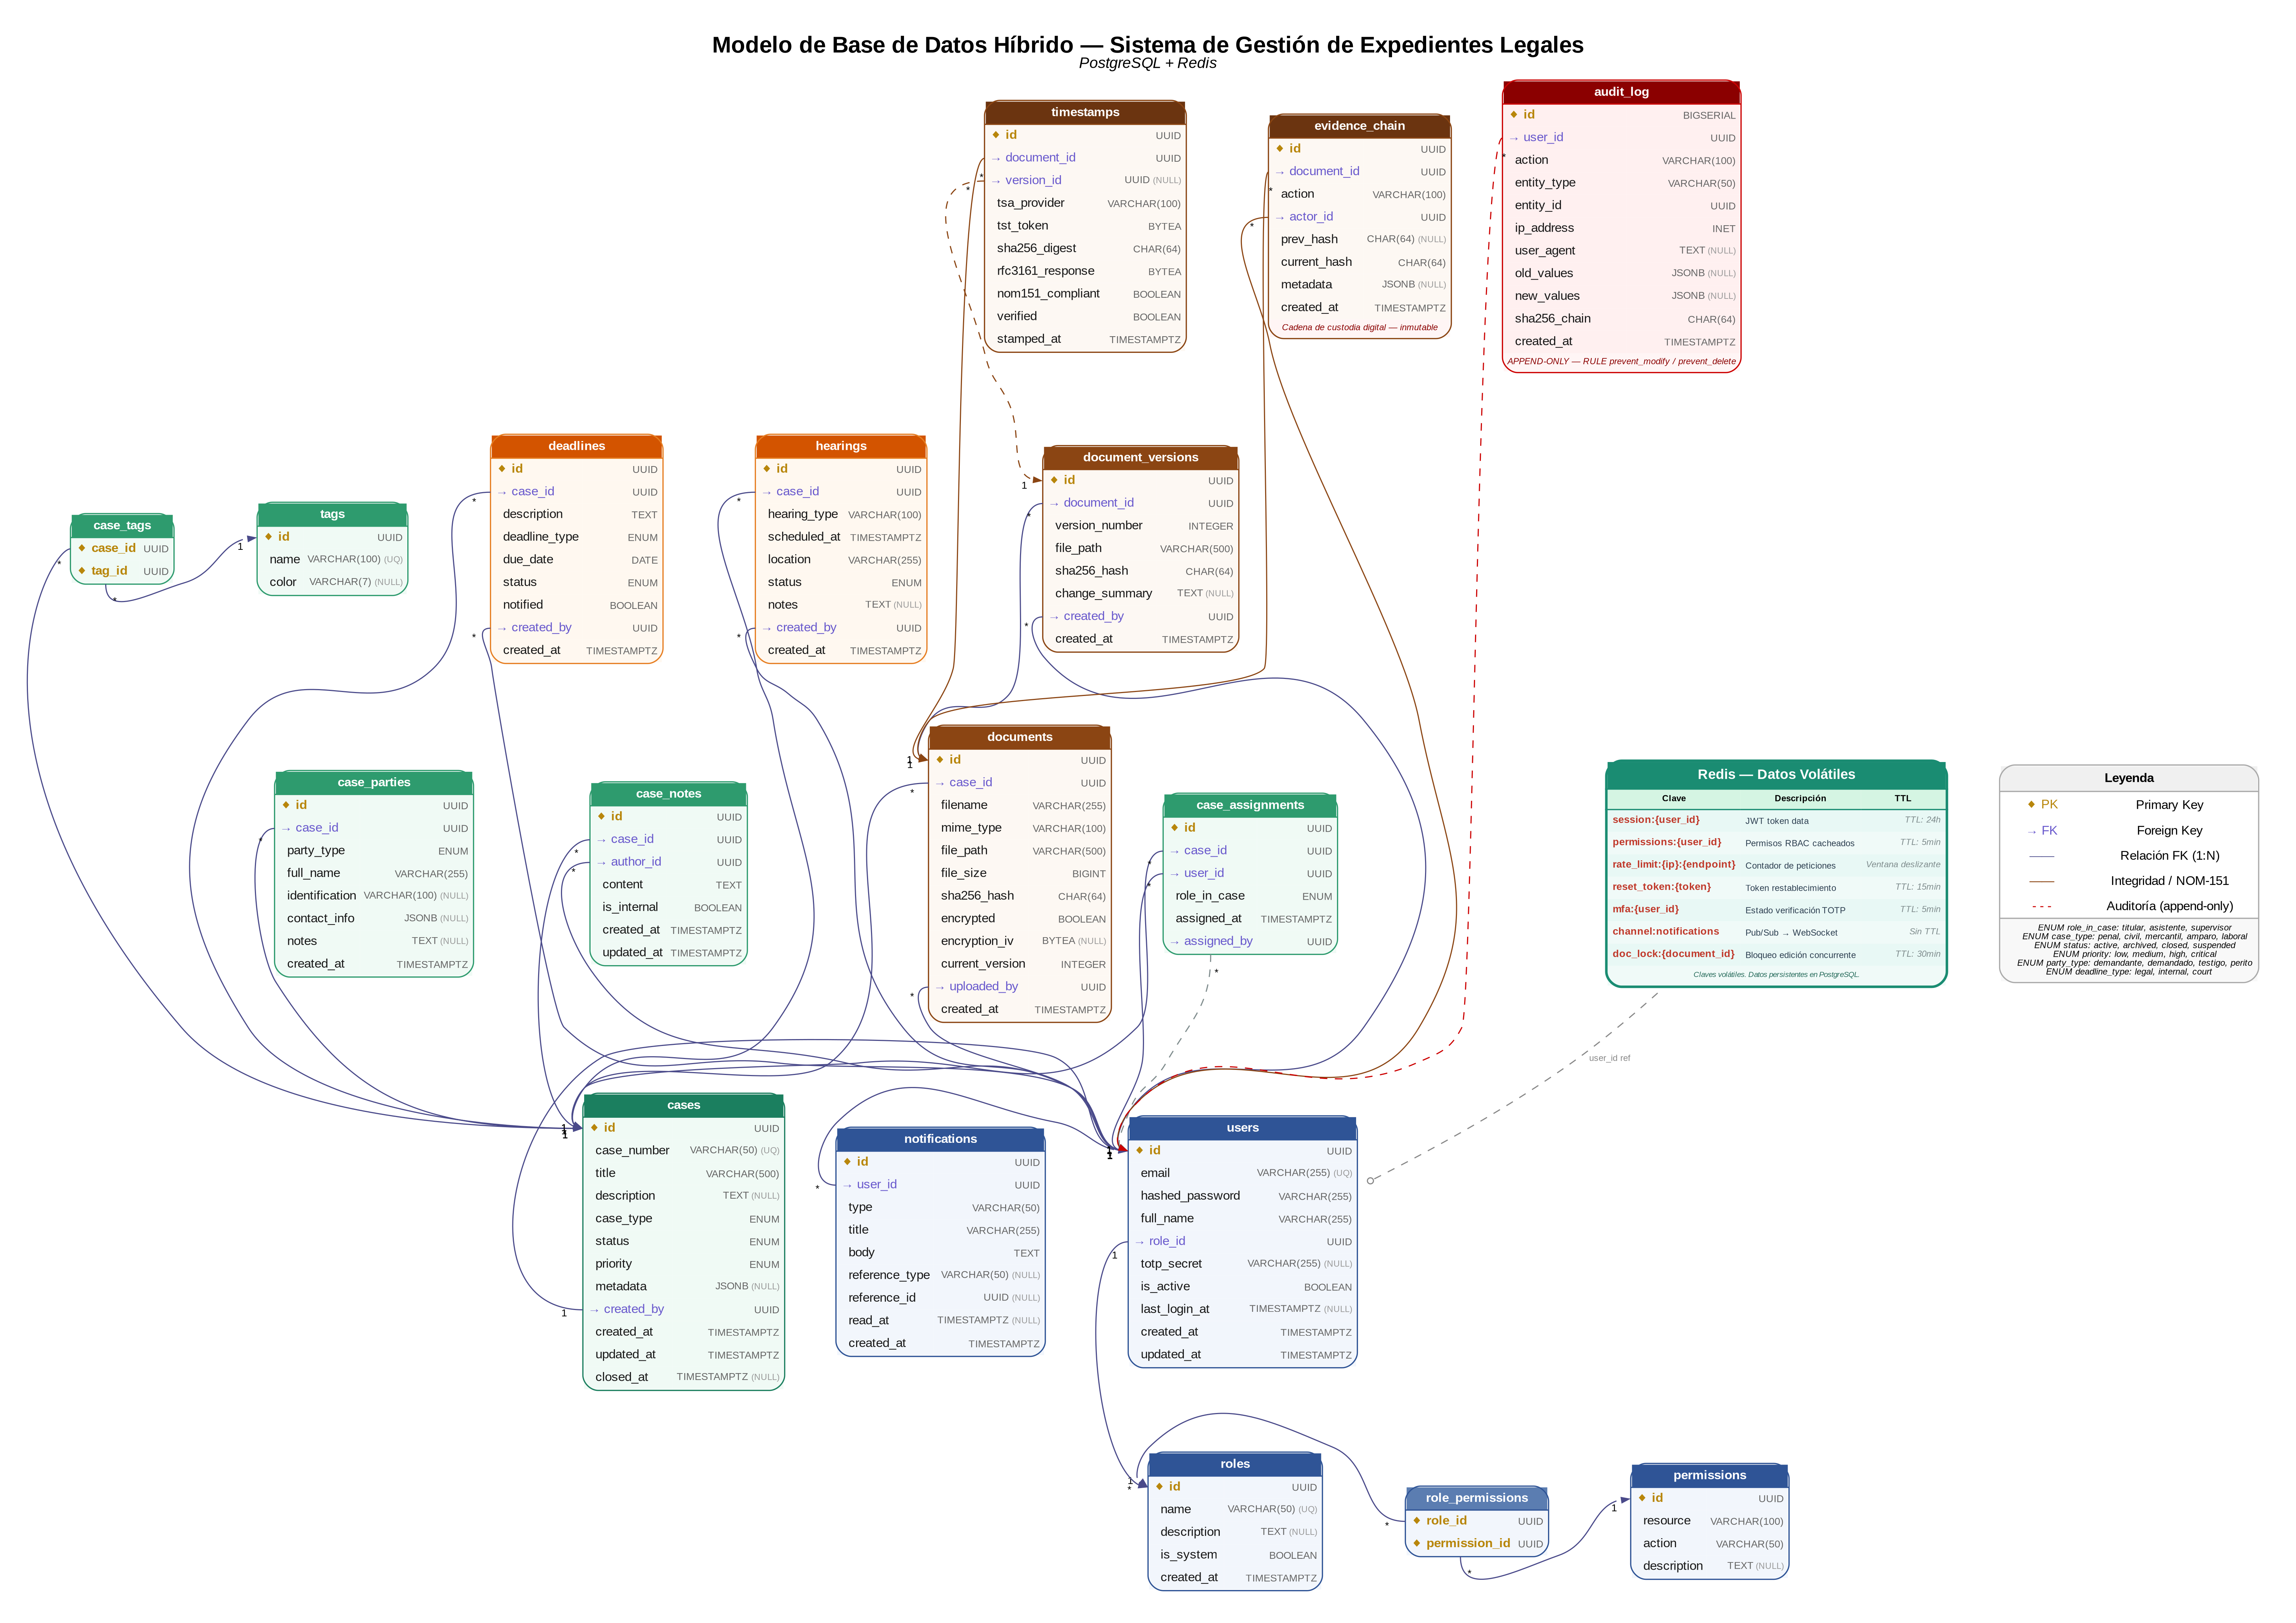
\includegraphics[width=0.9\linewidth]{image27.png}
  \caption{Modelo de datos híbrido: PostgreSQL para datos persistentes con valor probatorio, Redis para datos volátiles.}
  \label{fig:modelo-datos}
\end{figure}

Nótese que la tabla audit\_log está resaltada en rojo para indicar su naturaleza especial: es la única tabla del sistema con restricción RULE que impide UPDATE y DELETE. Su campo sha256\_chain implementa el encadenamiento criptográfico descrito en la \cref{sec:postgresql}. El campo metadata JSONB en la tabla cases permite almacenar atributos específicos de cada tipo de procedimiento sin necesidad de alterar el esquema relacional.

\section{Diagrama de Despliegue y Stack Tecnológico}\label{sec:despliegue}

La \cref{fig:despliegue} presenta la vista de despliegue del sistema, ilustrando la interacción entre las capas del frontend, el backend y los servicios de infraestructura.

\begin{figure}[H]
  \centering
  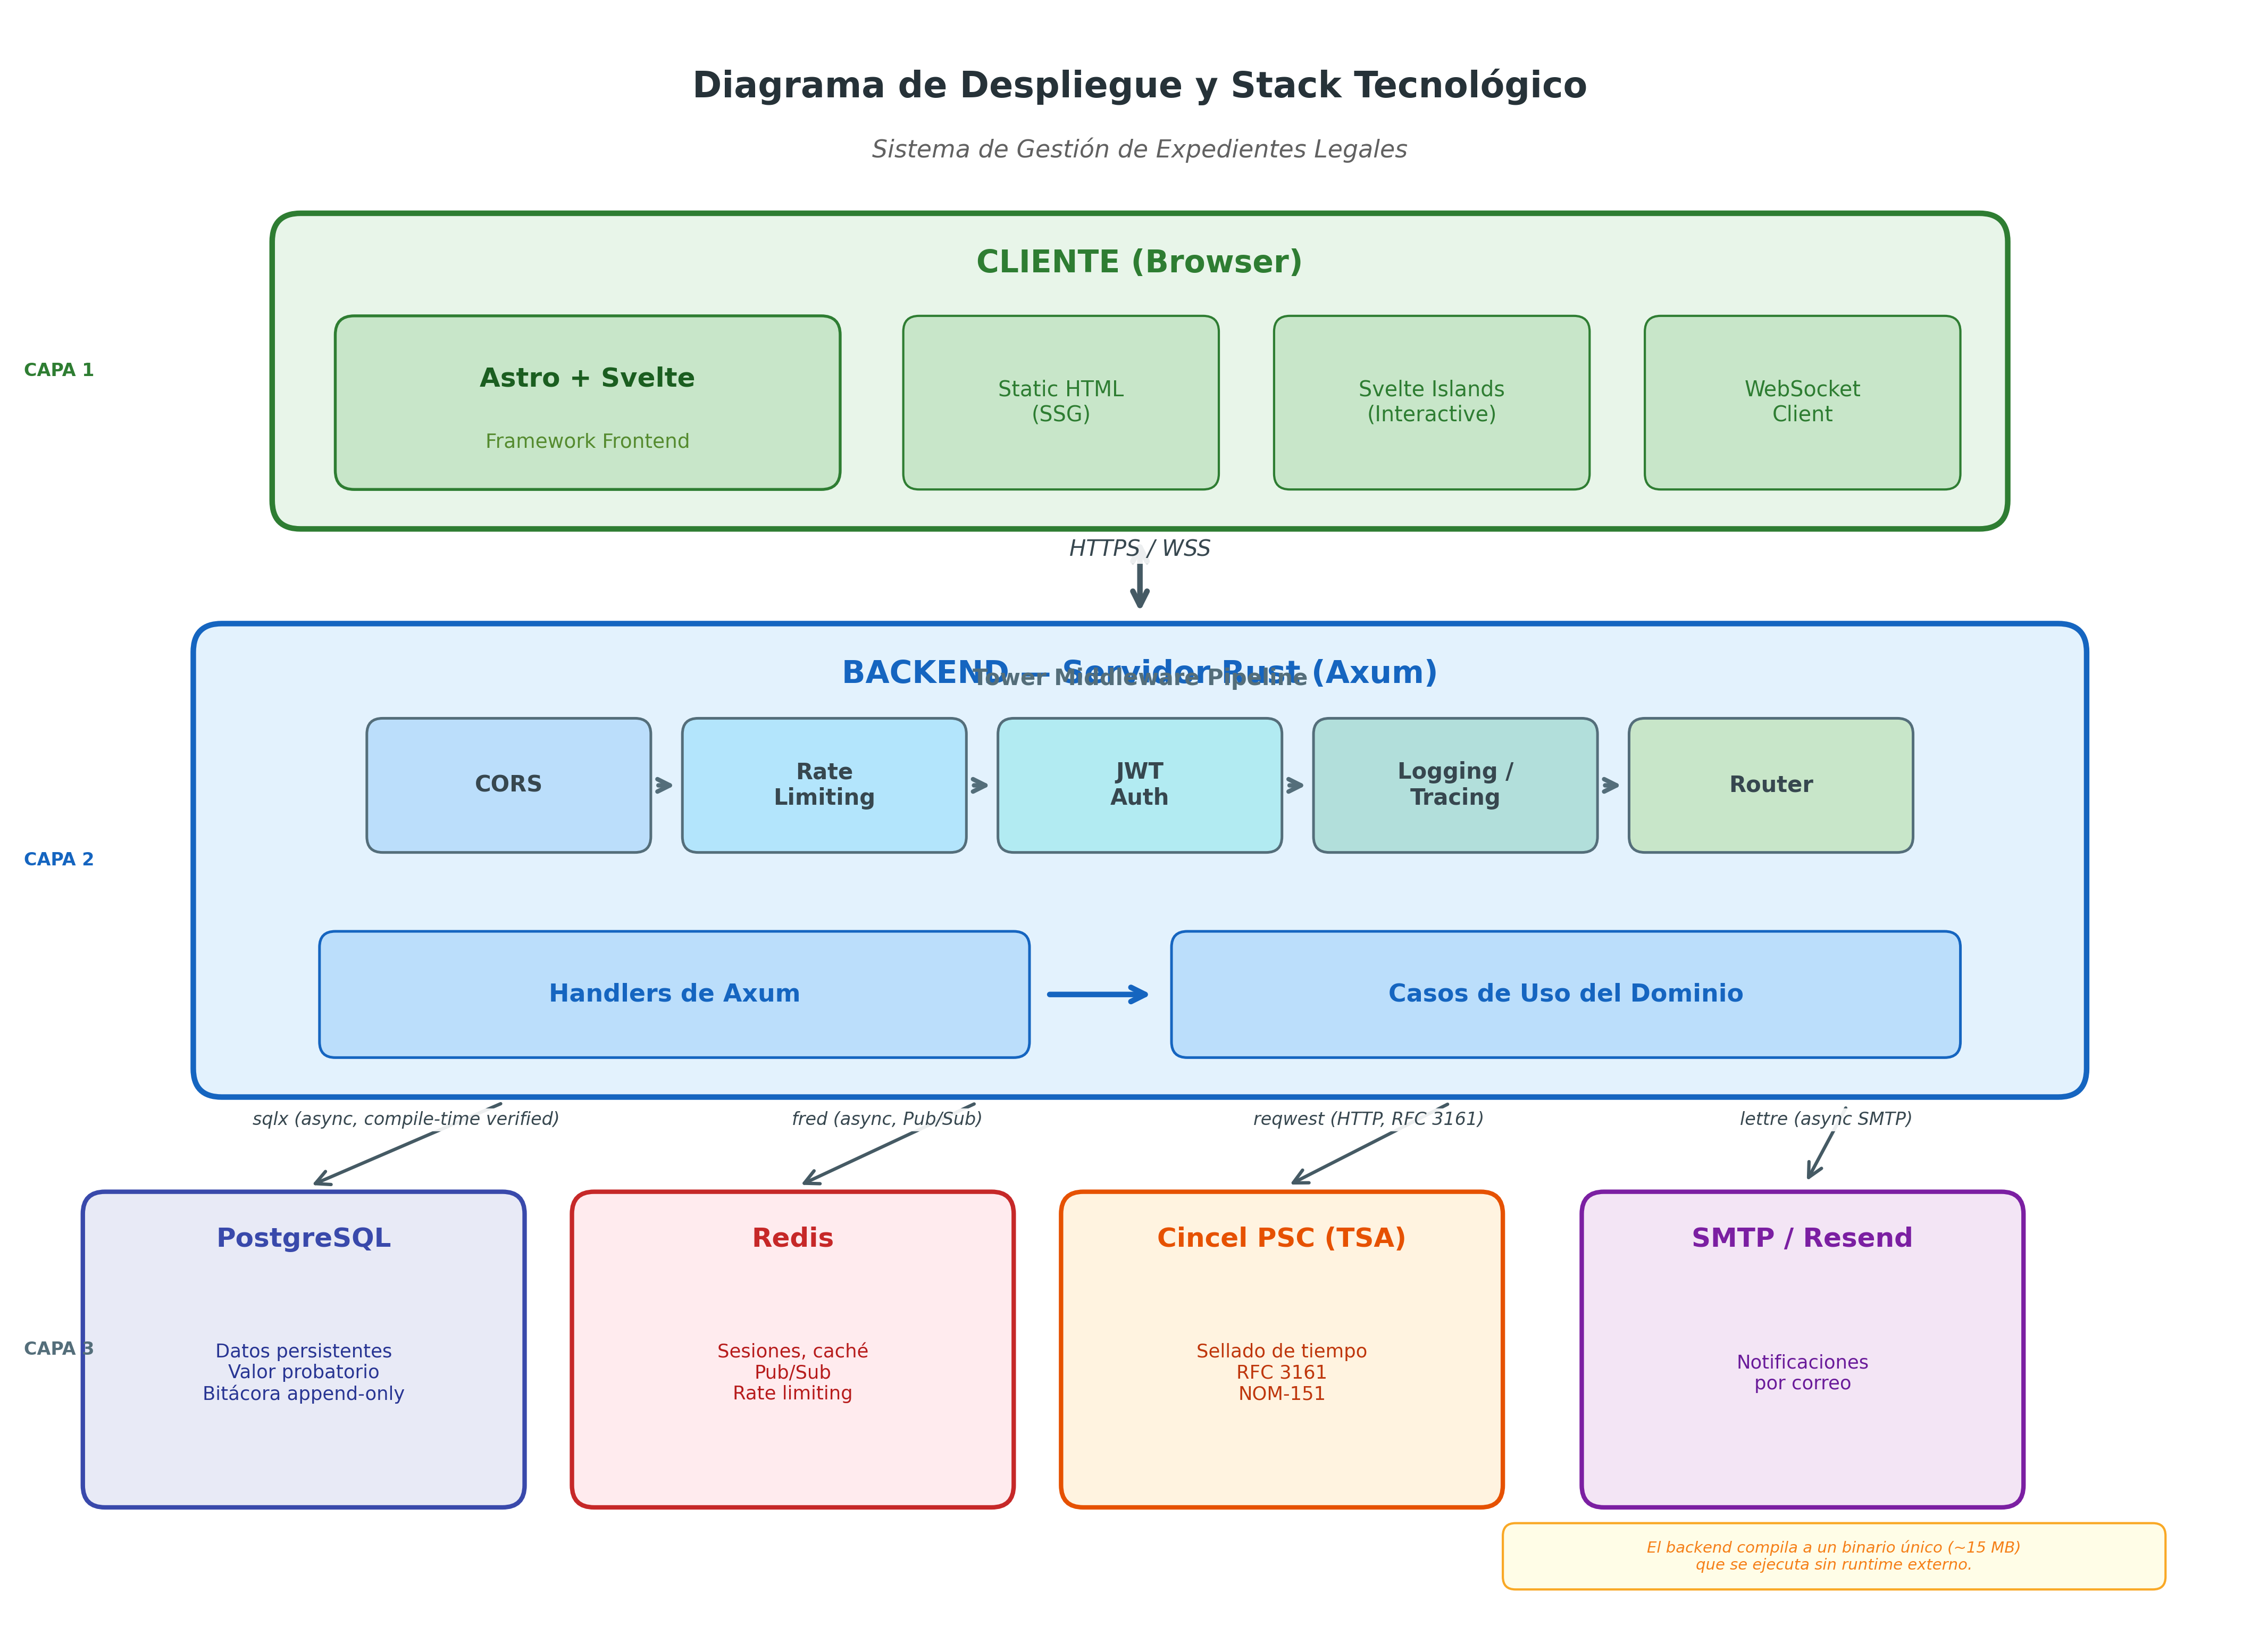
\includegraphics[width=0.9\linewidth]{image28.png}
  \caption{Diagrama de despliegue: Astro+Svelte (cliente) → Axum/Rust (backend) → PostgreSQL + Redis + servicios externos.}
  \label{fig:despliegue}
\end{figure}

El backend Rust compila a un \textbf{binario único} de aproximadamente 15 MB que incluye todas las dependencias. El binario Rust se ejecuta directamente sin runtime externo, eliminando la necesidad de intérpretes, servidores web adicionales o gestores de paquetes. Esto simplifica significativamente el despliegue y reduce la superficie de ataque del servidor.

La capa de \textbf{Tower Middleware} opera como un pipeline composable donde cada middleware es una capa que envuelve al siguiente. El flujo de una petición HTTP es: CORS → Rate Limiting → Autenticación JWT → Logging → Handler de Axum → Dominio. Esta composición es declarativa y verificada en tiempo de compilación por el sistema de tipos de Rust.

La comunicación con \textbf{Cincel PSC} para sellado de tiempo RFC 3161 se realiza a través de reqwest (cliente HTTP asíncrono). El diseño del puerto TimestampService como trait abstracto permite sustituir Cincel por cualquier otra TSA (SeguriData, CECOBAN; véase §2.3.3.4) implementando únicamente un nuevo adaptador, sin modificar el dominio ni los demás componentes del sistema.

Las conexiones a \textbf{PostgreSQL} se gestionan mediante sqlx, que ofrece verificación de queries SQL en tiempo de compilación contra el esquema real de la base de datos. Las conexiones a \textbf{Redis} se gestionan mediante fred, un cliente asíncrono compatible con cluster que soporta pub/sub nativo para las notificaciones en tiempo real.

\section{Modelo de Datos Jurídico-Técnico}\label{sec:modelo-juridico}

La fundamentación del proceso penal expuesta en el marco teórico tiene una consecuencia directa sobre el diseño del prototipo: la base de datos no puede ser un conjunto de tablas genéricas, sino que debe reflejar fielmente las dependencias y restricciones que el CNPP impone. Esta sección articula los vínculos explícitos entre la teoría jurídica y los requerimientos funcionales.

Un caso en el prototipo no es un registro estático, sino una entidad que evoluciona a través de los estados que el CNPP define como etapas \cite{cnpp2021}. La transición de un estado a otro solo es posible mediante la carga del documento procesal habilitante: de Investigación a Intermedia únicamente mediante el escrito de acusación; de Intermedia a Juicio Oral mediante el auto de apertura. El historial de transiciones debe mantenerse de forma inmutable como parte del expediente, dado que un tribunal revisor puede requerir verificar la secuencia procesal completa.

\section{Diseño Criptográfico del Prototipo}\label{sec:diseno-cripto}

Esta sección documenta las decisiones de diseño criptográfico adoptadas para el prototipo, fundamentadas en los conceptos teóricos expuestos en el capítulo 2 y en las restricciones impuestas por el marco legal mexicano. Cada decisión se justifica con referencia a los estándares y publicaciones del NIST, las RFC del IETF y las guías de OWASP que las sustentan.

\subsection{Nivel de Seguridad Objetivo}\label{sec:nivel-seguridad}

El prototipo adopta un nivel de fortaleza de seguridad de 128 bits conforme a NIST SP 800-57 Part 1 Rev 5 \cite{barker2020}. Este nivel unificado exige que cada primitivo criptográfico ofrezca al menos 128 bits de resistencia: SHA-256 proporciona 128 bits de resistencia a colisiones, AES-256 proporciona 256 bits de fortaleza, y RSA-3072 proporciona aproximadamente 128 bits. La elección de 128 bits como objetivo coherente garantiza que ningún eslabón de la cadena criptográfica sea más débil que los demás. NIST considera este nivel seguro al menos hasta 2030 para aplicaciones de uso general.

La Tabla 2 del NIST SP 800-57 \cite{barker2020} clasifica los niveles de fortaleza en función de los tamaños de clave recomendados para cada familia de algoritmos. El nivel de 112 bits, correspondiente a RSA-2048, está clasificado como legacy-use: aceptable para procesar información existente, pero no recomendado para proteger información nueva más allá de 2030. El nivel de 128 bits, correspondiente a RSA-3072, AES-128 o AES-256 y SHA-256, es el primer nivel que NIST clasifica como aceptable para uso general sin restricción temporal. Dado que el prototipo gestiona documentos con valor probatorio que pueden requerirse como prueba judicial años después de su firma, la elección del nivel de 128 bits proporciona un margen de seguridad adecuado frente a la evolución del poder computacional. Cabe señalar que la e.firma del SAT utiliza RSA-2048 (112 bits), un nivel inferior al adoptado por el prototipo; la libertad de elegir parámetros que otorga la CA interna permite superar ese piso normativo.

La coherencia entre primitivos se verifica de la siguiente manera: SHA-256 proporciona 128 bits de resistencia a colisiones y 256 bits de resistencia a preimagen; RSA-3072 proporciona aproximadamente 128 bits de fortaleza para firma digital; AES-256 proporciona 256 bits de fortaleza para cifrado simétrico, superando el nivel objetivo pero seleccionado por ser el tamaño estándar de clave para GCM en aplicaciones de nivel 128 bits o superior; y Argon2id con hash de salida de 32 bytes proporciona 256 bits de resistencia a preimagen para el almacenamiento de contraseñas. Ningún primitivo del sistema presenta una fortaleza inferior a 128 bits, lo que garantiza la ausencia de un eslabón débil en la cadena criptográfica. Esta propiedad de coherencia es especialmente relevante en un sistema que combina múltiples servicios criptográficos —integridad, confidencialidad, no repudio y autenticación—, ya que un atacante racional concentraría su esfuerzo en el primitivo más débil.

\subsection{Firma Digital}\label{sec:firma-digital}

El esquema de firma digital emplea RSA-3072 con SHA-256 y padding PKCS\#1 v1.5, con sha256\-With\-RSA\-Encryption como OID del algoritmo de firma. Se descartó ECDSA P-256 tras verificar que la Política de Certificados de la ACR2-SE \cite{economia_acr2se} establece que los certificados emitidos bajo la jerarquía PKI mexicana deben contener claves públicas RSA con sha256WithRSAEncryption como algoritmo de firma; ECDSA no está contemplado para certificados legalmente reconocidos bajo PSC mexicano. La elección de PKCS\#1 v1.5 sobre PSS se justifica por la alineación con el esquema que usa la PKI mexicana real (ACR2-SE y e.firma), lo que facilita la migración futura a certificados emitidos por un PSC sin rediseñar el verificador.

Los certificados X.509 v3 de los socios del despacho son emitidos por una Autoridad Certificadora (CA) interna del prototipo, implementada con OpenSSL scriptado en una topología de una sola capa: un certificado raíz autofirmado con vigencia de cinco años firma directamente los certificados de los socios con vigencia de un año. Esta elección expone al equipo al ciclo de vida completo de una PKI —generación de la clave raíz, emisión de CSRs (Certificate Signing Request, solicitudes de firma de certificado), firma de certificados, validación de cadena y revocación— que una integración con la e.firma del SAT o un PSC comercial ocultaría detrás de una API. El módulo de firma acepta cualquier certificado X.509 RSA + SHA-256, de modo que en un despliegue productivo la CA interna podría sustituirse por la e.firma o un PSC autorizado sin modificar la lógica de verificación.

La validación del estado de revocación se realiza mediante una Lista de Certificados Revocados (CRL) conforme a RFC 5280 \cite{cooper2008}, publicada como archivo PEM en el endpoint GET /pki/crl.pem con vigencia de siete días. La CRL se regenera bajo demanda tras cada revocación y periódicamente antes de su expiración. Se descartó OCSP por la escala reducida del prototipo (\textasciitilde{}2--5 certificados), donde la CRL es de tamaño despreciable y no requiere un servicio persistente adicional.

La elección de una CA interna sobre la e.firma del SAT o un PSC comercial responde a múltiples consideraciones. En primer lugar, las firmas generadas con certificados de la CA interna emplean los mismos mecanismos técnicos que las generadas con certificados de la e.firma o de un PSC: RSA-3072 con SHA-256, estructura X.509 v3 y verificación de cadena. Lo que cambia es el emisor y, con él, el nivel de confianza jurídica atribuible al certificado. Esta elección permite demostrar integridad y autoría dentro del alcance académico, pero no debe presentarse como equivalente a una firma avanzada. En segundo lugar, un sello RFC 3161 emitido por un PSC autorizado puede aportar la independencia temporal prevista por la NOM-151 \cite{adams2001,nom151_2016}; un sello emitido por la TSA interna conserva el mismo flujo criptográfico, pero permanece dentro de la frontera de confianza del prototipo.

En tercer lugar, usar la e.firma habría obligado a que el socio subiera su archivo .key y su contraseña al prototipo, o a implementar firma del lado del cliente parseando el formato propietario del SAT. Ambas rutas introducen un problema de custodia de claves que contradice el objetivo declarado de no repudio: si el servidor custodia la clave privada del firmante, la firma pierde su propiedad vinculante porque no puede atribuirse exclusivamente a su titular. Con la CA interna, el ciclo de vida de las claves queda bajo control del prototipo y es auditable. Finalmente, montar la CA internamente expone al equipo al ciclo de vida completo de una PKI —generación de la clave raíz, emisión de CSRs, firma de certificados con extensiones X.509 v3, construcción de la cadena de confianza, validación y revocación— que una integración con la e.firma o un PSC comercial ocultaría detrás de una API externa. Este aprendizaje es parte del valor formativo declarado del Trabajo Terminal.

La implementación de la CA se realiza con OpenSSL scriptado en lugar de herramientas como step-ca o EJBCA. OpenSSL expone cada paso del proceso de forma transparente y auditable: la generación de la clave raíz (openssl genrsa), la creación del certificado autofirmado (openssl req -x509), la firma de solicitudes de certificado (openssl x509 -req -CA) y la generación de CRLs (openssl ca -gencrl) se encapsulan en aproximadamente cuatro invocaciones cuyo resultado es verificable con openssl x509 -text. step-ca automatiza y oculta esa mecánica detrás de una API REST, lo cual es deseable en producción pero contraproducente para un ejercicio académico. Además, OpenSSL no introduce dependencias adicionales al stack del prototipo. Respecto a las vigencias, el certificado raíz tiene una validez de cinco años para sobrevivir ampliamente al ciclo de vida del proyecto y al período de evaluación, mientras que los certificados de los socios tienen una validez de un año, alineada con la práctica estándar de la industria y suficiente para demostrar que el prototipo contempla la renovación de certificados.

\subsection{Sellado de Tiempo}\label{sec:sellado-tiempo}

El sellado de tiempo se diseña detrás del puerto \texttt{TimestampService}, con \texttt{LocalOpensslTsa} como adaptador actual de demostración y un adaptador de PSC externo como sustitución futura. En ambos casos el flujo opera conforme al protocolo RFC 3161 \cite{adams2001}: se calcula el hash SHA-256 del documento firmado, se solicita el sello al emisor configurado y se almacena la respuesta \texttt{TimeStampResp} en formato ASN.1 DER como artefacto independiente (.tsr). Esta abstracción permite sustituir la TSA local por Cincel, SeguriData, CECOBAN u otra TSA compatible sin modificar la lógica central. La equivalencia es de protocolo, no de confianza: únicamente el camino hacia un PSC autorizado y contratado puede producir la constancia externa prevista por la NOM-151-SCFI-2016.

Para facilitar la verificación independiente por un tercero (tribunal, contraparte, perito), el prototipo genera un paquete ZIP descargable que contiene el documento original, la firma RSA del socio, el sello de tiempo .tsr, los certificados del firmante y de la CA raíz, e instrucciones con comandos OpenSSL para la verificación completa. Este diseño garantiza que la verificación no dependa de la disponibilidad de la plataforma.

La selección inicial de Cincel como proveedor de sellado de tiempo obedeció a tres factores. Primero, Cincel es un PSC acreditado por la Secretaría de Economía para la emisión de Sellos Digitales de Tiempo (SDT) y constancias de conservación de mensajes de datos (CCMD), con acreditación publicada en el Diario Oficial de la Federación el 24 de noviembre de 2023 \cite{comparasoftware2026}. Segundo, ofrece un entorno de sandbox y recursos de integración. Tercero, la interfaz documentada permite enviar el hash SHA-256 y recuperar el artefacto ASN.1 DER conforme a RFC 3161 \cite{cincel2024,adams2001}, incluidos estados de procesamiento diferido que el prototipo maneja mediante reintentos configurables. La experiencia de integración corrigió la segunda premisa: aunque el registro se completó, el sandbox requiere pago con precios no transparentes y la API no ofreció respuesta y estabilidad suficientes para una campaña repetible. En consecuencia, Cincel no se utiliza como evidencia de esta entrega; permanece únicamente como adaptador externo opcional, mientras la TSA interna verifica el flujo completo sin convertir la disponibilidad comercial en requisito de desarrollo.

El sello de tiempo se almacena como la respuesta cruda \texttt{TimeStampResp} en formato ASN.1 DER (extensión .tsr) en lugar de empaquetarlo en una estructura CAdES-T o embebido en un PDF (PAdES-T). Esta decisión se justifica por tres razones. Primera, con artefactos independientes cada componente del flujo criptográfico —documento, firma, sello, certificado— puede inspeccionarse y verificarse por separado con herramientas estándar; el comando \texttt{openssl ts -verify} opera directamente sobre archivos .tsr sin necesidad de parsear contenedores CMS ni estructuras PDF. Segunda, CAdES-T requeriría construir estructuras CMS con atributos no firmados y PAdES-T requeriría manipular los mecanismos internos del formato PDF (\texttt{ByteRange}, diccionarios de firma y guardados incrementales), tareas de ingeniería de formatos que consumirían tiempo del cronograma sin aportar al objetivo criptográfico del Trabajo Terminal. Tercera, el contenedor no altera el token RFC 3161 subyacente ni la identidad de su emisor: el alcance jurídico depende de la autoridad y su cadena de confianza, no de almacenar el token como .tsr, CAdES-T o PAdES-T \cite{nom151_2016}.

El flujo de verificación completo del sello de tiempo procede en cuatro pasos: (1) se parsea la \texttt{TimeStampResp} para extraer el \texttt{TimeStampToken}; (2) se verifica que \texttt{messageImprint.\allowbreak{}hashedMessage} coincida con el hash SHA-256 recalculado del documento original; (3) se verifica la firma de la TSA sobre el token; y (4) se valida su certificado contra el ancla de confianza correspondiente. Para la TSA interna, esa ancla es la CA del prototipo; para una constancia externa, debe ser la cadena del PSC emisor hasta la ACR2-SE \cite{economia_acr2se}. Con OpenSSL, el proceso se ejecuta con \texttt{openssl ts -verify -data documento.pdf -in sello.tsr -CAfile ancla.pem}. Un despliegue productivo podría migrar a CAdES-T o PAdES-T sin cambiar el token subyacente ni el flujo de obtención.

\subsection{Cifrado en Reposo}\label{sec:cifrado-reposo}

Los documentos almacenados se cifran con AES-256-GCM conforme a NIST SP 800-38D \cite{dworkin2007}. Cada operación utiliza un nonce (número de uso único) aleatorio de 96 bits generado con un CSPRNG (Generador de Números Pseudoaleatorios Criptográficamente Seguro), cuya probabilidad de colisión es despreciable cuando cada documento emplea su propia clave (NIST SP 800-38D §8.3 establece un límite de 2³² invocaciones por clave). La gestión de claves sigue un esquema de envelope encryption: una Clave de Cifrado de Clave (KEK), almacenada en una variable de entorno del servidor, envuelve una Clave de Cifrado de Datos (DEK) generada aleatoriamente para cada documento conforme a NIST SP 800-38F \cite{dworkin2012}. Esta separación permite rotar la KEK re-cifrando únicamente las DEKs envueltas, sin necesidad de re-cifrar los documentos del repositorio. Los Datos Adicionales Autenticados (AAD) de GCM incluyen el identificador del documento y su versión, lo que previene ataques de intercambio (swap) y de reversión (rollback) entre documentos.

La elección de un nonce aleatorio sobre un nonce de contador responde a la prioridad de evitar el modo de fallo más catastrófico de GCM: la reutilización de un par (clave, nonce). Un nonce de contador requiere mantener un estado persistente que se incremente atómicamente en cada operación de cifrado; si ese estado se reinicia por un error de software, una restauración de respaldo o una condición de carrera, el contador repite un valor y el esquema GCM se rompe irrecuperablemente, exponiendo tanto el texto claro como la clave de autenticación. Un nonce aleatorio de 96 bits generado con un CSPRNG elimina esta dependencia de estado por diseño: cada invocación es independiente y no requiere coordinación con invocaciones anteriores. NIST SP 800-38D \cite{dworkin2007} §8.3 establece que con nonces aleatorios de 96 bits el número total de invocaciones por clave no debe exceder 2³² (aproximadamente 4,300 millones) para mantener la probabilidad de colisión por debajo de \textasciitilde{}2⁻³³. Con envelope encryption, donde cada documento emplea su propia DEK, el número de invocaciones por clave es efectivamente uno, lo que hace la probabilidad de colisión exactamente cero en la práctica.

La arquitectura de envelope encryption se seleccionó sobre dos alternativas: una clave única compartida para todo el repositorio y una derivación de claves mediante HKDF. Una sola clave compartida concentra el riesgo —su compromiso expone la totalidad de la información— y hace la rotación prohibitivamente costosa porque cada documento debe re-cifrarse. Un esquema basado en HKDF derivaría una clave por documento a partir de una clave maestra y un contexto único (por ejemplo, el identificador del documento), lo que evita almacenar claves envueltas pero presenta dos desventajas: si la clave maestra se compromete, todas las claves derivadas caen sin posibilidad de revocar una sola; y la unicidad absoluta del contexto de derivación reintroduce un problema de estado similar al del nonce de contador. Envelope encryption aísla el daño por diseño: el compromiso de una DEK solo expone un documento, y el compromiso de la KEK requiere además acceso al almacenamiento cifrado para descifrar las DEKs. Este es el patrón estándar de la industria, implementado por AWS KMS, Google Cloud KMS y Azure Key Vault \cite{dworkin2012}.

El flujo de cifrado procede de la siguiente manera al almacenar un documento: (1) se genera una DEK aleatoria de 32 bytes con un CSPRNG; (2) se genera un nonce aleatorio de 12 bytes; (3) se cifra el documento con AES-256-GCM utilizando la DEK, el nonce y los AAD (document\_id + version), obteniendo el ciphertext y un authentication tag de 16 bytes; (4) se genera un segundo nonce de 12 bytes para la envoltura; y (5) se cifra la DEK con la KEK usando AES-256-GCM. El paquete cifrado del documento se almacena en formato nonce (12 bytes) ‖ ciphertext ‖ tag (16 bytes), y la DEK envuelta sigue el mismo formato. El flujo de descifrado invierte el proceso: primero se descifra la DEK con la KEK verificando la integridad del tag, y después se descifra el documento con la DEK recuperada. Si cualquiera de los dos tags falla la verificación, la operación se rechaza íntegramente, lo que previene la entrega de documentos corrompidos o manipulados.

La rotación de la KEK es una operación ligera que no requiere re-cifrar ningún documento. Al generar una nueva KEK con un CSPRNG, se itera sobre las DEKs del repositorio: cada una se descifra con la KEK vigente y se re-cifra con la nueva. Dado que las DEKs son bloques de 32 bytes, esta operación es de tamaño fijo y se ejecuta en tiempo constante por documento, independientemente del tamaño del documento protegido. Los documentos en sí no se tocan: sus DEKs no cambian, solo cambia su envoltura. Esta separación es la ventaja principal de envelope encryption sobre un esquema de clave única: la rotación opera sobre claves (rápida, de tamaño fijo) y no sobre documentos (potencialmente de varios megabytes). Para el prototipo, basta con implementar y documentar el mecanismo de rotación; ejecutar una rotación periódica queda fuera del alcance de la demostración.

\subsection{Autenticación y Control de Acceso}\label{sec:autenticacion}

Las contraseñas de los usuarios se almacenan hasheadas con Argon2id (RFC 9106) \cite{biryukov2015,biryukov2021}, la variante híbrida recomendada por OWASP \cite{owasp_pwstorage2024} y NIST SP 800-63B Rev 4 \cite{nist2024} para nuevas implementaciones. Los parámetros adoptados son: memoria m = 256 MiB (262\,144 KiB), iteraciones t = 4, paralelismo p = 1, sal de 16 bytes y hash de salida de 32 bytes. En el hardware de referencia (AMD Ryzen 7 7730U, 16 hilos lógicos) cinco corridas promediaron 607.8 ms, dentro de la banda objetivo de 0.5--1.0 segundo por intento legítimo. Si el hardware de despliegue difiere, la medición debe repetirse antes de la puesta en producción.

Los clientes del despacho cuentan adicionalmente con autenticación de doble factor mediante TOTP (RFC 6238) \cite{mraihi2011,owasp_mfa2024} con HMAC-SHA1, códigos de 6 dígitos, período de 30 segundos y secreto de 20 bytes, alcanzando el nivel AAL2 de NIST SP 800-63B \cite{nist2024}. Se descartó WebAuthn/FIDO2 (AAL3) por la barrera de adopción que representa para clientes de un despacho legal que requiere solo un smartphone con una app autenticadora estándar. Los socios, por su parte, se autentican mediante certificados digitales X.509 emitidos por la CA interna (\cref{sec:firma-digital}), lo que provee un nivel de aseguramiento equivalente a AAL3 sin hardware dedicado adicional.

La selección de Argon2id sobre bcrypt se fundamenta en la propiedad de dureza de memoria (memory-hardness). bcrypt, diseñado en 1999, es resistente a fuerza bruta en CPU gracias a su costo iterativo, pero utiliza únicamente aproximadamente 4 KiB de memoria por invocación, lo que permite a un atacante con GPUs o ASICs ejecutar miles de instancias en paralelo a bajo costo por unidad de intento. Argon2id obliga a reservar 256 MiB por cada intento de hash en la configuración calibrada, lo que hace que escalar el ataque con hardware masivo sea prohibitivamente caro porque la memoria DRAM es el recurso que peor escala en paralelo. Argon2 fue el ganador de la Password Hashing Competition (PHC) en julio de 2015 \cite{biryukov2015}, una competencia abierta de dos años con 24 candidatos evaluados por un panel de criptógrafos. Esta validación pública es análoga a la que AES recibió del concurso NIST en 2001 y aporta confianza en que el diseño ha sido ampliamente escrutado.

Argon2 define tres variantes que difieren en su resistencia a distintos vectores de ataque. Argon2d maximiza la resistencia a ataques con GPU y ASIC, pero es vulnerable a ataques de canal lateral si el atacante puede observar los patrones de acceso a memoria del proceso. Argon2i es resistente a ataques de canal lateral al usar un patrón de acceso independiente de los datos, pero ofrece ligeramente menos resistencia a hardware especializado. Argon2id es la variante híbrida: ejecuta Argon2i en el primer pase para proteger contra canal lateral, y Argon2d en los pases subsiguientes para maximizar la resistencia a GPU. RFC 9106 \cite{biryukov2021} §4 recomienda explícitamente Argon2id para hashing de contraseñas por esta combinación de protecciones. Los parámetros adoptados (m = 256 MiB, t = 4, p = 1, sal de 16 bytes, hash de 32 bytes) fueron seleccionados por calibración del hardware de referencia; la sal de 128 bits excede el mínimo de 64 bits de RFC 9106 y es el valor recomendado por OWASP.

La selección de HMAC-SHA1 como función base del TOTP merece una justificación explícita dado que SHA-1 está desaconsejado para firmas digitales desde 2017 por la demostración práctica de colisiones. Sin embargo, la seguridad de HMAC no depende de la resistencia a colisiones de la función hash subyacente, sino de la pseudoaleatoriedad de su función de compresión interna. NIST SP 800-107 Rev 1 \cite{dang2012} confirma que HMAC-SHA-1 sigue siendo aceptable para autenticación de mensajes y generación de códigos. Adicionalmente, HMAC-SHA1 es el único algoritmo soportado universalmente por todas las aplicaciones autenticadoras del mercado; Google Authenticator históricamente solo soporta SHA-1, lo que haría que la adopción de HMAC-SHA256 o HMAC-SHA512 excluyera a una parte significativa de los dispositivos de los clientes del despacho.

El flujo de registro (enrollment) del segundo factor procede de la siguiente manera: (1) el cliente inicia sesión con usuario y contraseña; (2) el sistema genera un secreto de 20 bytes con un CSPRNG; (3) se codifica como URI otpauth (otpauth://totp/Despacho:cliente@email?secret=BASE32(secret)) y se presenta como código QR; (4) el cliente escanea con su aplicación autenticadora; (5) el cliente ingresa el código actual para confirmar la configuración; y (6) el sistema almacena el secreto cifrado con AES-256-GCM y genera ocho códigos de recuperación de un solo uso, hasheados con Argon2id antes de almacenarse. Durante la autenticación, el sistema calcula el TOTP esperado para tres ventanas temporales (t₀₋₁, t₀, t₀₊₁), lo que tolera un desfase de reloj de hasta 30 segundos entre servidor y dispositivo. Se aplica rate limiting de cinco intentos fallidos consecutivos con bloqueo temporal de 15 minutos para prevenir fuerza bruta en línea sobre el espacio de 10⁶ combinaciones (6 dígitos).

\subsection{Postura Legal del Prototipo}\label{sec:postura-legal}

La firma generada por el prototipo constituye una firma electrónica simple conforme al artículo 89 del Código de Comercio \cite{ccom2018}, dado que los certificados no provienen de un PSC autorizado (artículo 97, requisito 5). Su argumentación probatoria se apoya en: (1) la admisibilidad de la firma simple como prueba, ya que el artículo 89 no condiciona la admisibilidad a la intervención de un PSC; y (2) la cláusula de equivalencia funcional del artículo 100, que permite argumentar la fiabilidad del método con base en estándares reconocidos internacionalmente (RSA-3072 conforme a NIST SP 800-57 \cite{barker2020} y SHA-256 conforme a FIPS 180-4 \cite{nist2015fips1804}). Un sello emitido por un PSC autorizado añadiría fecha cierta e independencia de tercero conforme al marco de la NOM-151; el token de la TSA interna demuestra el mecanismo RFC 3161, pero no añade esa garantía externa. La distinción práctica respecto de una firma avanzada radica en la carga de la prueba: quien invoca la firma simple debe acreditar la fiabilidad del método, mientras que la firma avanzada goza de presunción legal. En un despliegue productivo, la sustitución de la CA interna por un PSC autorizado convertiría la firma en avanzada sin cambios arquitectónicos, dado que el módulo de firma acepta cualquier certificado X.509 RSA + SHA-256.

La arquitectura del prototipo está diseñada para que la transición de firma simple a firma avanzada sea una operación de configuración, no de rediseño. El módulo de firma define una interfaz abstracta que acepta cualquier certificado X.509 con clave RSA y algoritmo sha256WithRSAEncryption. En un despliegue productivo, el despacho podría sustituir la CA interna por certificados emitidos por un PSC autorizado como SeguriData \cite{seguridata} o CECOBAN \cite{cecoban}, convirtiendo la firma en avanzada conforme al artículo 97 del Código de Comercio \cite{ccom2018}; o bien integrar la e.firma del SAT si los socios ya disponen de ella, sin modificar la lógica de verificación. De forma análoga, el módulo de sellado de tiempo define una interfaz abstracta que permite sustituir Cincel por cualquier TSA que implemente RFC 3161 \cite{adams2001}. Esta portabilidad del emisor es un acierto arquitectónico deliberado: el prototipo demuestra la corrección de los mecanismos criptográficos con una infraestructura soberana del despacho, mientras que la producción puede adoptar la infraestructura regulada sin tocar el código de verificación.

% =====================================================================
%  04-implementacion.tex — Capitulo 4: Implementacion del prototipo
% =====================================================================

\chapter{Implementación del prototipo}\label{cap:implementacion}

Este capítulo documenta la implementación del prototipo cuyo análisis y diseño se presentó en el Capítulo~\ref{cap:analisis}. La implementación conserva la dirección de dependencias de ese diseño: el sistema se construyó como un workspace de Cargo de cinco crates con la regla de dependencias de la arquitectura hexagonal impuesta por el grafo de compilación (\cref{sec:workspace-cargo}), y cada uno de los servicios criptográficos especificados en el diseño criptográfico (\cref{sec:diseno-cripto}) se materializó mediante puertos de dominio, casos de uso y adaptadores concretos de infraestructura, tal como anticipó la definición de la arquitectura hexagonal (\cref{sec:hexagonal-definicion}). El capítulo se organiza en seis secciones. La primera describe la estructura real del workspace y el andamiaje de calidad que lo rodea: perfil de compilación, configuración, telemetría, integración continua y política de dependencias. La segunda recorre los diez servicios criptográficos implementados, identificando para cada uno su puerto, su adaptador, los crates empleados y las decisiones técnicas registradas. La tercera presenta la interfaz de línea de comandos que expone los casos de uso. La cuarta documenta la aplicación HTTP autenticada, PostgreSQL, Redis y la persistencia documental cifrada. La quinta reporta los resultados de la exploración del sellado de tiempo, el componente que el análisis de riesgos señaló como el de mayor exposición (\cref{sec:riesgos-tecnicos}). La sexta registra las divergencias respecto al diseño del Capítulo~\ref{cap:analisis} y las decisiones de arquitectura documentadas durante la construcción.

\section{Estructura del workspace y andamiaje}\label{sec:impl-workspace}

\textbf{Estado implementado al 12 de septiembre de 2026.} El prototipo expone una API Axum multiusuario con alta inicial, autenticación Argon2id, TOTP o recuperación, sesiones revocables, expedientes y asignaciones. Las operaciones documentales exigen un expediente y comprueban el acceso tanto antes de preparar el resultado como al confirmarlo. PostgreSQL persiste usuarios, expedientes, pertenencias, documentos cifrados y una cadena de auditoría compartida; Redis conserva el estado efímero de autenticación. Están implementados carga, sellado local, verificación y exportación de evidencia. Permanecen pendientes la interfaz de producto, las consultas e historial de versiones documentales y la actividad procesal.

{\emergencystretch=2em El prototipo es un workspace de Cargo con cinco crates miembros bajo \rutarepo{crates/}: \texttt{domain}, \texttt{application}, \texttt{infrastructure}, \texttt{web} y \texttt{bin}, conforme a la estructura de \cref{sec:workspace-cargo}. La dirección de dependencias apunta al dominio: \texttt{domain} no depende de otro crate del workspace; \texttt{application} depende de \texttt{domain}; \texttt{infrastructure} y \texttt{web} dependen de las dos capas interiores; y \texttt{bin}, raíz de composición que produce \texttt{despacho-cli}, depende de todas. Este último es el único crate que utiliza \texttt{anyhow} en la frontera del proceso. HTTP consume los puertos de aplicación \texttt{Identity\allowbreak Workflow}, \texttt{Case\allowbreak Workflow} y \texttt{Case\allowbreak Document\allowbreak Workflow}, sin conocer los adaptadores concretos. La \cref{tab:impl-crates} sintetiza las responsabilidades; las pruebas unitarias viven en \texttt{src} y las de integración en \texttt{tests/}. La convención de mantenimiento limita a menos de 400 líneas cada archivo de código, según \texttt{CONTRIBUTING.md}.\par}

\begin{table}[H]
  \centering
  \caption{Responsabilidades de los crates del workspace.}
  \label{tab:impl-crates}
  \begin{tabularx}{\linewidth}{@{}l X X@{}}
    \toprule
    \textbf{Crate} & \textbf{Responsabilidad} & \textbf{Elementos del flujo integrado} \\
    \midrule
    \texttt{domain} & Valores, reglas, puertos y errores; sin E/S & Identidad, expedientes, permisos, criptografía y cadena de auditoría. \\
    \texttt{application} & Casos de uso y fronteras de persistencia & Autenticación, asignaciones y operaciones documentales por expediente. \\
    \texttt{infrastructure} & Adaptadores de servicios y almacenamiento & PostgreSQL, Redis, cifrado, firma, TSA, ZIP e importación local. \\
    \texttt{web} & Adaptador HTTP y DTO & Extracción de peticiones, rutas, errores y límites de concurrencia. \\
    \texttt{bin} & Composición y comandos & Servidor, preparación de esquema, importación y herramientas offline. \\
    \bottomrule
  \end{tabularx}
\end{table}

La regla de dependencias no descansa en la disciplina del equipo sino en dos mecanismos verificables. El primero es el propio grafo de Cargo: como se argumentó en el diseño (\cref{sec:workspace-cargo}), una importación prohibida produce un error de compilación, no una advertencia de revisión. El segundo es una prueba de arquitectura, \rutarepo{crates/bin/tests/architecture.rs}, que lee el manifiesto del crate \texttt{domain} y falla si este declara dependencia alguna de \texttt{application}, \texttt{infrastructure} o \texttt{web}; esta prueba protege contra la degradación gradual del manifiesto, que el compilador no reportaría mientras los símbolos prohibidos no se usen. Una segunda prueba estructural, \rutarepo{crates/bin/tests/port_coverage.rs}, recorre el workspace y exige que cada \texttt{pub trait} del dominio ---cada puerto--- tenga al menos un adaptador (\texttt{impl <Trait> for}) en \texttt{infrastructure} y al menos un mock generado con \texttt{mockall} en los tests; para detectar un escáner degradado, la prueba usa puertos centinela (\texttt{AuditLog}, \texttt{Document\allowbreak Hasher}, \texttt{KeyManager}) cuya ausencia delataría un análisis roto.

La versión mínima soportada del compilador es Rust 1.88, declarada mediante \texttt{rust-version} en el \texttt{Cargo.toml} raíz y comprobada por un job obligatorio de integración continua. La elevación desde 1.78 permite adoptar correcciones de seguridad de \texttt{time} y de la familia PostgreSQL, conforme a \rutarepo{docs/adr/0013-raise-msrv-for-security-fixes.md}. Se conserva la familia de APIs construida alrededor de \texttt{der}~0.7 ---\texttt{x509-cert}~0.2, \texttt{cms}~0.2, \texttt{x509-tsp}~0.1 y \texttt{rsa}~0.9--- porque su sustitución exige una migración coordinada, no porque 1.78 siga siendo el requisito vigente. Las dependencias compartidas se declaran en \texttt{[workspace.dependencies]}. El perfil de release aplica \texttt{strip = true} y \texttt{lto = true}; en desarrollo se optimizan los núcleos \texttt{argon2}, \texttt{blake2}, \texttt{num-bigint-dig} y \texttt{rsa}, manteniendo información de depuración en el resto del workspace.

La configuración se carga desde variables de entorno con \texttt{dotenvy} (archivo \texttt{.env} local, nunca versionado; la plantilla comentada \texttt{.env.example} sí lo está). La \cref{tab:impl-env} lista las variables. Dos decisiones de manejo de secretos son transversales: la carga de configuración registra en la bitácora únicamente la \emph{presencia} de cada variable, jamás su valor; y todo material secreto leído del entorno o de la entrada estándar (la KEK, la credencial del proveedor de sellado, las contraseñas) aterriza en buffers \texttt{Zeroizing} que sobrescriben su contenido al liberarse, conforme al ADR \rutarepo{docs/adr/0003-zeroize-secret-material-in-domain.md}.

\begin{table}[H]
  \centering
  \caption{Variables de entorno del prototipo (plantilla \texttt{.env.example}).}
  \label{tab:impl-env}
  \begin{tabularx}{\linewidth}{@{}l X@{}}
    \toprule
    \textbf{Variable} & \textbf{Propósito} \\
    \midrule
    \texttt{RUST\_LOG} & Filtro de severidad de la telemetría (por defecto \texttt{info}). \\
    \texttt{CINCEL\_BASE\_URL} & URL base del proveedor remoto de sellado de tiempo. \\
    \texttt{CINCEL\_API\_KEY} & Credencial del proveedor de sellado (secreto; se llena localmente). \\
    \texttt{DATABASE\_URL} & PostgreSQL para usuarios, expedientes, documentos y auditoría; conexión administrativa para migrar y rol restringido para servir. \\
    \texttt{REDIS\_URL} & Cadena de conexión Redis para sesiones, desafíos y límites. \\
    \texttt{KEK\_BASE64} & Clave de cifrado de claves: 32 bytes aleatorios en base64 (secreto). \\
    \texttt{NEW\_KEK\_BASE64} & KEK de reemplazo; la lee únicamente \texttt{vault rotate-kek}. \\
    \texttt{AUDIT\_LOG\_PATH} & Ruta de la bitácora offline; HTTP usa PostgreSQL (por defecto \texttt{audit-log.jsonl}). \\
    \texttt{PKI\_CA\_DIR} & Directorio de trabajo de la CA interna (por defecto \texttt{pki-ca}). \\
    \texttt{TSA\_DIR} & Directorio de trabajo de la TSA local (por defecto \texttt{pki-tsa}). \\
    \bottomrule
  \end{tabularx}
\end{table}

La telemetría usa \texttt{tracing} y \texttt{tracing-subscriber} con filtro por entorno, materializando la observabilidad estructurada prevista en el diseño (\cref{sec:observabilidad}). Todos los diagnósticos se emiten por la salida de error estándar, de modo que la salida estándar queda limpia para resultados y tuberías de shell. La promesa de que ningún secreto aparece en los diagnósticos no es una convención: la prueba \rutarepo{crates/bin/tests/log_redaction.rs} ejecuta los flujos con el nivel de log más verboso e inspecciona lo emitido, fallando si algún material secreto conocido aparece en la salida de error.

El workflow de integración continua ejecuta siete jobs en cada push y pull request (\cref{tab:impl-ci}). La comprobación de MSRV es obligatoria y usa Rust 1.88. Los jobs de pruebas y cobertura preparan PostgreSQL y Redis y separan las bases de identidad, expedientes y documentos, de modo que las pruebas de persistencia no se omiten por ausencia de configuración. El umbral de \rutarepo{scripts/coverage-gate.sh} exige 90\,\% de líneas por crate en \texttt{domain}, \texttt{application} e \texttt{infrastructure}; \texttt{bin} se reporta sin bloquear. Estos valores son criterios de aceptación configurados, no mediciones de una ejecución concreta.

\begin{table}[H]
  \centering
  \caption{Jobs del workflow de integración continua.}
  \label{tab:impl-ci}
  \begin{tabularx}{\linewidth}{@{}l l X@{}}
    \toprule
    \textbf{Job} & \textbf{Herramienta} & \textbf{Criterio de aprobación} \\
    \midrule
    format & \texttt{cargo fmt} & Formato canónico en todo el workspace. \\
    lint & \texttt{cargo clippy} & Cero advertencias (\texttt{-D warnings}). \\
    test & \texttt{cargo test} & Suite completa del workspace en verde. \\
    msrv & \texttt{cargo check} & Compila con Rust 1.88; comprobación obligatoria. \\
    coverage & \texttt{cargo-llvm-cov} & $\geq$ 90\,\% de líneas por crate criptográfico. \\
    deny & \texttt{cargo-deny} & Avisos, licencias, duplicados y fuentes en regla. \\
    binary-size & \texttt{cargo build -{}-release} & \texttt{despacho-cli} $\leq$ 25~MB. \\
    \bottomrule
  \end{tabularx}
\end{table}

El diseño comprometió cinco fitness functions como verificaciones automatizadas de los atributos de calidad (\cref{sec:fitness-functions}) \cite{ford2023}. La \cref{tab:impl-fitness} muestra dónde vive cada una en el repositorio. Cuatro de las cinco diseñadas se implementaron directamente; la función que exige un span de \texttt{tracing} por handler HTTP sigue pendiente aun cuando los handlers ya existen, y en su lugar se incorporó el umbral de cobertura por crate como función de aptitud adicional.

\begin{table}[H]
  \centering
  \caption{Fitness functions implementadas y su ubicación en el repositorio.}
  \label{tab:impl-fitness}
  \begin{tabularx}{\linewidth}{@{}l L{6.4cm} X@{}}
    \toprule
    \textbf{Id} & \textbf{Propiedad verificada} & \textbf{Verificación implementada} \\
    \midrule
    FF-1 & El dominio no depende de capas externas & Grafo de Cargo en cada build y \rutarepo{crates/bin/tests/architecture.rs}. \\
    FF-2 & Ningún log contiene material secreto & \rutarepo{crates/bin/tests/log_redaction.rs} al nivel de log más verboso. \\
    FF-3 & Todo puerto tiene adaptador y mock & \rutarepo{crates/bin/tests/port_coverage.rs} con puertos centinela. \\
    FF-4 & Cobertura $\geq$ 90\,\% en crates criptográficos & \rutarepo{scripts/coverage-gate.sh} sobre el reporte de \texttt{cargo-llvm-cov}. \\
    FF-5 & Binario release $\leq$ 25~MB & Job \texttt{binary-size} del workflow de integración continua. \\
    \bottomrule
  \end{tabularx}
\end{table}

La política de dependencias revisa avisos, licencias, duplicados y fuentes del grafo. Se configura en \texttt{deny.toml} para \texttt{cargo-deny} y en \texttt{audit.toml} para \texttt{cargo-audit}. Permanece declarada la excepción RUSTSEC-2023-0071 \cite{rustsec2023_0071}, relativa a temporización en operaciones de clave privada del crate \texttt{rsa}. El razonamiento original de \rutarepo{docs/adr/0002-rsa-signing-crate-and-advisory.md} suponía firma por CLI; esa premisa no describe la exposición HTTP actual. La autenticación y los límites de concurrencia acotan quién puede solicitar firmas y cuántas se ejecutan, pero no corrigen el canal lateral. Antes de un despliegue público se requiere revisar el modelo de amenaza y resolver la elección del firmante. La API local no se presenta como una configuración de producción validada.

\section{Servicios criptográficos}\label{sec:impl-servicios}

El diseño criptográfico del Capítulo~\ref{cap:analisis} (\cref{sec:diseno-cripto}) especificó los servicios de integridad, confidencialidad, no repudio y autenticación del prototipo. Esta sección los recorre como diez servicios implementados, S1 a S10, cada uno con la misma anatomía: un puerto (trait) en \texttt{domain}, un adaptador en \texttt{infrastructure} y un caso de uso en \texttt{application} que los orquesta. La \cref{tab:impl-servicios} presenta el mapa completo. Dos convenciones atraviesan todos los servicios. Primera: los rechazos criptográficos son \emph{resultados} tipados (enumeraciones como \texttt{Signature\allowbreak Verification} o \texttt{Certificate\allowbreak Validation}), nunca errores; el camino de error queda reservado a fallos del backend o a evidencia inevaluable, lo que permite construir políticas futuras ---por ejemplo, bloqueo de cuenta--- sin confundir un intento fallido con una falla del sistema. Segunda: la delegación a la herramienta \texttt{openssl} como subproceso ocurre en exactamente tres puntos ---la CA interna, la TSA local y la etapa criptográfica del verificador RFC 3161---; todo lo demás es Rust nativo sobre \texttt{ring}, \texttt{rsa}, \texttt{sha2}, \texttt{x509-cert}, \texttt{cms}, \texttt{x509-tsp}, \texttt{argon2} y \texttt{totp-rs}.

El manejo de errores materializa el patrón de errores tipados por capa que el diseño estableció (\cref{sec:manejo-errores}). El crate de dominio define \texttt{DomainError} (\rutarepo{crates/domain/src/error.rs}) con 26 variantes tipadas mediante \texttt{thiserror}, una por condición de fallo con significado propio ---longitud de digest inválida, payload sellado malformado, CRL vencida, nombre de entrada de archivo inutilizable---. Una variante merece mención explícita: \texttt{Authentication\allowbreak Failed}, el rechazo de un descifrado autenticado, es deliberadamente opaca y no revela si falló la clave, el tag o los datos, negando a un adversario la retroalimentación que distingue esos casos. Los errores de los backends de infraestructura (\texttt{CryptoError}, \texttt{TsaError}) se convierten hacia el dominio mediante conversiones \texttt{From}, y la capa de aplicación añade en \texttt{Application\allowbreak Error} solo lo que le es propio: el fallo genérico de un puerto, un archivo vault malformado y un certificado recién emitido que no supera su validación posterior a la emisión.

\begin{table}[H]
  \centering
  \caption{Servicios criptográficos implementados: puertos del dominio y adaptadores de infraestructura.}
  \label{tab:impl-servicios}
  \begin{tabularx}{\linewidth}{@{}l L{3.4cm} L{4.6cm} X@{}}
    \toprule
    \textbf{Id} & \textbf{Servicio} & \textbf{Puerto(s) del dominio} & \textbf{Adaptador(es)} \\
    \midrule
    S1 & Hash de documentos & \texttt{Document\allowbreak Hasher} & \texttt{Ring\allowbreak Sha256\allowbreak Hasher} \\
    S2 & Cifrado autenticado y envelope encryption & \texttt{Authenticated\allowbreak Cipher}, \texttt{KeyManager} & \texttt{Ring\allowbreak Aes\allowbreak Gcm\allowbreak Cipher}, \texttt{Envelope\allowbreak Key\allowbreak Manager} \\
    S3 & PKI interna & \texttt{Certificate\allowbreak Authority}, \texttt{Certificate\allowbreak Validator} & \texttt{Openssl\allowbreak Ca\allowbreak Adapter}, \texttt{X509\allowbreak Chain\allowbreak Validator} \\
    S4 & Firma digital & \texttt{Document\allowbreak Signer}, \texttt{Signature\allowbreak Verifier} & \texttt{Rsa\allowbreak Pkcs1\allowbreak Signer}, \texttt{Rsa\allowbreak Pkcs1\allowbreak Verifier} \\
    S5 & Sellado de tiempo & \texttt{Timestamp\allowbreak Service}, \texttt{Timestamp\allowbreak Verifier} & \texttt{Local\allowbreak Openssl\allowbreak Tsa}, \texttt{Cincel\allowbreak Tsa\allowbreak Adapter}, \texttt{Rfc3161\allowbreak Verifier} \\
    S6 & Verificación integral & (compone los de S1, S3, S4 y S5) & caso de uso \texttt{Verify\allowbreak Document} \\
    S7 & Hash de contraseñas & \texttt{Password\allowbreak Hasher} & \texttt{Argon2id\allowbreak Hasher} \\
    S8 & Segundo factor TOTP & \texttt{Totp\allowbreak Provider}, \texttt{Recovery\allowbreak Code\allowbreak Generator} & \texttt{Totp\allowbreak Rs\allowbreak Provider}, \texttt{Random\allowbreak Recovery\allowbreak Code\allowbreak Generator} \\
    S9 & Cadena de auditoría & \texttt{AuditLog}, \texttt{Clock} & \texttt{Postgres\allowbreak Audit\allowbreak Log}, \texttt{File\allowbreak Audit\allowbreak Log}, \texttt{SystemClock} \\
    S10 & Paquete de evidencia & \texttt{Archive\allowbreak Writer} & \texttt{Stored\allowbreak Zip\allowbreak Writer} \\
    \bottomrule
  \end{tabularx}
\end{table}

\subsection{S1. Hash de documentos con SHA-256}\label{sec:impl-s1-hash}

El puerto \texttt{Document\allowbreak Hasher} (\rutarepo{crates/domain/src/crypto/hasher.rs}) es el más simple del sistema y sirve para ilustrar el patrón que repiten todos los demás: un trait del dominio que declara el contrato criptográfico sin nombrar backend alguno. El Listado~\ref{lst:impl-puerto-hasher} lo reproduce íntegro.

\begin{lstlisting}[language=Rust,caption={Puerto de hashing del dominio (\texttt{crates/domain/src/crypto/hasher.rs}).},label={lst:impl-puerto-hasher}]
/// Computes SHA-256 digests of document content.
///
/// Adapters implement this port with a concrete cryptographic backend. Both
/// operations must produce the same digest for the same input bytes.
pub trait DocumentHasher {
    /// Hashes a byte slice already held in memory.
    fn hash_bytes(&self, data: &[u8]) -> Sha256Digest;

    /// Hashes a stream by consuming it in fixed-size blocks, so inputs of
    /// any length are digested without loading them fully into memory.
    ///
    /// # Errors
    ///
    /// Returns [`DomainError::StreamRead`] when reading from `reader` fails.
    fn hash_stream(&self, reader: &mut dyn Read) -> Result<Sha256Digest, DomainError>;
}
\end{lstlisting}

El adaptador \texttt{Ring\allowbreak Sha256\allowbreak Hasher} (\rutarepo{crates/infrastructure/src/hashing.rs}) lo implementa con el crate \texttt{ring}~0.17. La variante de flujo consume la entrada en bloques de 64~KiB, de modo que el consumo de memoria es plano para entradas de cualquier tamaño, y reintenta las lecturas interrumpidas por señales del sistema operativo. El resultado es el value object \texttt{Sha256\allowbreak Digest}, un arreglo fijo de 32 bytes con constructores que rechazan longitudes o codificaciones hexadecimales inválidas. Siguiendo la práctica de desarrollo guiado por pruebas del proyecto, los primeros tests del adaptador son los vectores oficiales de FIPS 180-4 \cite{nist2015fips1804}, complementados con una verificación de interoperabilidad contra \texttt{sha256sum} y con propiedades verificadas por generación aleatoria de casos. El caso de uso \texttt{Hash\allowbreak Document} expone el servicio a la interfaz de usuario.

\subsection{S2. Cifrado autenticado y envelope encryption}\label{sec:impl-s2-cifrado}

{\emergencystretch=2em La confidencialidad en reposo diseñada en \cref{sec:cifrado-reposo} se implementa con dos puertos. El primero, \texttt{Authenticated\allowbreak Cipher} (\rutarepo{crates/domain/src/crypto/cipher.rs}), declara las operaciones de sellado y apertura autenticados; el material de clave cruza la interfaz como slices de bytes para que el crate de dominio permanezca libre de dependencias criptográficas, mientras los buffers propietarios viven en contenedores \texttt{Zeroizing} del lado del llamador. Su adaptador, \texttt{Ring\allowbreak Aes\allowbreak Gcm\allowbreak Cipher} (\rutarepo{crates/infrastructure/src/encryption.rs}), implementa AES-256-GCM con \texttt{ring} \cite{dworkin2007,mcgrew2008}: en cada operación de sellado se extrae un nonce fresco de 96 bits del CSPRNG del sistema, y la salida adopta el formato fijo nonce~(12~bytes)~$\Vert$~criptograma~$\Vert$~tag~(16~bytes), representado por el value object \texttt{Sealed\allowbreak Payload}, que rechaza cualquier secuencia menor a 28 bytes. Todo rechazo de descifrado se colapsa deliberadamente en el error opaco \texttt{Authentication\allowbreak Failed}, que no revela si falló la clave, el tag o los datos.\par}

Los datos adicionales autenticados ligan cada criptograma a la identidad y versión del documento, tal como exigió el diseño para prevenir ataques de intercambio y de reversión. La función de dominio \texttt{document\_aad} (Listado~\ref{lst:impl-document-aad}) construye ese vínculo: 16 bytes crudos del UUID del documento seguidos de la versión como 4 bytes big-endian.

\begin{lstlisting}[language=Rust,caption={Construcción del AAD que liga el criptograma a su documento (\texttt{crates/domain/src/crypto/cipher.rs}).},label={lst:impl-document-aad}]
/// Builds the additional authenticated data that binds a sealed document to
/// its identity: the 16 raw bytes of the document id UUID followed by the
/// document version as 4 big-endian bytes.
///
/// Sealing a document with this AAD makes decryption fail unless the caller
/// asks for exactly the same document and version. That prevents
/// substituting one document's ciphertext for another's (the id would
/// differ) and replaying an older version of the same document (the version
/// would differ).
pub fn document_aad(id: DocumentId, version: DocumentVersion) -> [u8; DOCUMENT_AAD_LEN] {
    let mut aad = [0u8; DOCUMENT_AAD_LEN];
    aad[..16].copy_from_slice(id.as_uuid().as_bytes());
    aad[16..].copy_from_slice(&version.get().to_be_bytes());
    aad
}
\end{lstlisting}

El segundo puerto, \texttt{KeyManager} (\rutarepo{crates/domain/src/crypto/keys.rs}), gobierna el esquema de envelope encryption \cite{dworkin2012}: generar una DEK, envolverla bajo la KEK, desenvolverla y re-envolverla bajo una KEK nueva. Su adaptador \texttt{Envelope\allowbreak Key\allowbreak Manager} genera una DEK aleatoria de 32 bytes por documento y la sella con el mismo cifrador AES-256-GCM, pero con AAD \emph{vacío}: la decisión, documentada en el propio código, es que la DEK envuelta ya queda ligada a su documento por el archivo que la transporta, y mantener la envoltura independiente de la identidad permite rotar la KEK re-envolviendo todas las claves sin necesidad de saber a qué documento pertenece cada una. El caso de uso \texttt{Encrypt\allowbreak Document} serializa el resultado en el formato de archivo \texttt{DVLT1} (\cref{tab:impl-vault}), definido normativamente en \rutarepo{crates/application/src/vault.rs}; \texttt{Decrypt\allowbreak Document} reconstruye el AAD con la identidad y versión que el llamador afirma, de modo que un identificador o versión incorrectos fallan exactamente igual que un criptograma alterado; y \texttt{RotateKek} re-envuelve únicamente la DEK, copiando intactos los bytes del documento sellado, con un costo independiente del tamaño del documento ---la propiedad de rotación que el diseño exigió en \cref{sec:cifrado-reposo}.

\begin{table}[H]
  \centering
  \caption[Formato del archivo vault \texttt{DVLT1}]{Formato del archivo vault \texttt{DVLT1} (definición normativa en \texttt{crates/application/src/vault.rs}).}
  \label{tab:impl-vault}
  \begin{tabularx}{\linewidth}{@{}l l X@{}}
    \toprule
    \textbf{Desplazamiento} & \textbf{Tamaño} & \textbf{Campo} \\
    \midrule
    0 & 5 & Bytes mágicos ASCII \texttt{DVLT1}. \\
    5 & 4 & Longitud $N$ (big-endian) de la DEK envuelta. \\
    9 & $N$ & DEK envuelta: nonce~$\Vert$~criptograma~$\Vert$~tag, sellada bajo la KEK con AAD vacío. \\
    $9+N$ & resto & Documento sellado: nonce~$\Vert$~criptograma~$\Vert$~tag, sellado bajo la DEK con AAD = identificador del documento (16 bytes UUID)~$\Vert$~versión (4 bytes big-endian). \\
    \bottomrule
  \end{tabularx}
\end{table}

\subsection{S3. Infraestructura de clave pública interna}\label{sec:impl-s3-pki}

La CA interna de una sola capa especificada en \cref{sec:firma-digital} se implementó como un conjunto de scripts versionados bajo \rutarepo{pki/} ---\texttt{init-ca.sh}, \texttt{issue-cert.sh}, \texttt{revoke.sh}, \texttt{gen-crl.sh}--- que operan la herramienta OpenSSL con configuración declarativa (\texttt{openssl.cnf}). Los parámetros coinciden con el diseño: claves RSA de 3\,072 bits, firma sha256WithRSAEncryption en todos los casos, certificado raíz autofirmado con vigencia de 1\,825 días (cinco años), certificados de entidad final con vigencia de 365 días y CRL con vigencia de siete días conforme a RFC 5280 \cite{cooper2008}. La política de emisión obliga a que país y organización del certificado emitido coincidan con los de la CA, ignora las extensiones solicitadas en el CSR (\texttt{copy\_extensions = none}) y aplica un retroceso deliberado de cinco minutos al inicio de vigencia ---práctica común de las autoridades públicas--- para que un certificado sea utilizable de inmediato aun con desfase de reloj entre máquinas. El puerto \texttt{Certificate\allowbreak Authority} se implementa en \texttt{Openssl\allowbreak Ca\allowbreak Adapter} (\rutarepo{crates/infrastructure/src/certificates/authority.rs}), que ejecuta esos scripts como subprocesos con el directorio de trabajo inyectado vía \texttt{PKI\_CA\_DIR} y normaliza los números de serie a hexadecimal en mayúsculas antes de invocar subproceso alguno. El caso de uso \texttt{Issue\allowbreak Certificate} rehúsa reportar éxito hasta validar el certificado recién emitido contra la raíz, de modo que una CA mal inicializada falla en la emisión y no en el primer uso. Los scripts operan con disciplina defensiva ---\texttt{set -euo pipefail}, verificación previa de que \texttt{openssl} está disponible, inicialización idempotente que rehúsa sobrescribir una CA existente--- y el material de claves privadas jamás se versiona: vive únicamente en el directorio de trabajo en tiempo de ejecución, con el \texttt{.gitignore} del repositorio como red de seguridad adicional; el \texttt{README.md} del directorio documenta el orden de uso, los comandos de verificación independiente y la versión de OpenSSL (3.5.7) con la que fueron probados.

La validación es el puerto \texttt{Certificate\allowbreak Validator}, implementado por \texttt{X509\allowbreak Chain\allowbreak Validator} (\rutarepo{crates/infrastructure/src/certificates/validator.rs}). Las crates \texttt{x509-cert}~0.2 y \texttt{der}~0.7 solo \emph{parsean} X.509 y deliberadamente no verifican firmas, así que la verificación criptográfica se implementó re-codificando a DER la estructura to-be-signed parseada y comprobando la firma PKCS\#1 v1.5 con \texttt{rsa} y \texttt{sha2} contra la clave pública del emisor ---la misma técnica para la firma de la CRL sobre su \texttt{tbsCertList}---, decisión registrada en \rutarepo{docs/adr/0004-certificate-validation-implementation.md} y correcta porque DER es una codificación canónica: decodificar y re-codificar entrada DER válida reproduce los bytes firmados. El validador ejecuta sus comprobaciones en orden fijo y reporta exactamente el primer fallo: (1) confianza del emisor ---nombre, algoritmo y firma---; (2) ventana de vigencia del certificado; (3) ventana de vigencia \emph{del emisor}, porque un emisor fuera de su propia vigencia no ancla confianza en ese instante; y (4) revocación contra la CRL opcional. El contrato de revocación es estricto: si se presenta una CRL, cualquier defecto de la lista ---ilegible, no firmada por el emisor, o vencida en su \texttt{nextUpdate}--- es un error duro y nunca un pase permisivo; omitir la CRL es una decisión explícita del llamador que el reporte de verificación hace visible. El instante de evaluación siempre es un timestamp explícito, lo que permite a las pruebas controlar el reloj.

\subsection{S4. Firma digital RSA-3072}\label{sec:impl-s4-firma}

El esquema de firma es el diseñado en \cref{sec:firma-digital}: RSA-3072 con SHA-256 y padding PKCS\#1 v1.5. Los puertos son \texttt{Document\allowbreak Signer} y \texttt{Signature\allowbreak Verifier} (\rutarepo{crates/domain/src/crypto/signature.rs}); nunca se firma el documento sino su digest SHA-256, calculado por el puerto de hashing, y el rechazo de una verificación es un resultado tipado, no un error. Los adaptadores \texttt{Rsa\allowbreak Pkcs1\allowbreak Signer} y \texttt{Rsa\allowbreak Pkcs1\allowbreak Verifier} (\rutarepo{crates/infrastructure/src/signing.rs}) usan los crates \texttt{rsa}~0.9 y \texttt{sha2}~0.10 con la feature \texttt{oid}, que liga SHA-256 a su identificador en la estructura DigestInfo del padding, de modo que los 32 bytes ya calculados se firman sin hashear dos veces. El firmador rechaza en construcción cualquier módulo menor a 3\,072 bits; acepta la clave privada en PEM PKCS\#8 o PKCS\#1, la retiene en un buffer \texttt{Zeroizing}, la parsea únicamente durante la operación de firma y la descarta al salir del ámbito, y su representación de depuración omite el material (\texttt{private key pem withheld}). El verificador acepta como material de clave tanto un certificado X.509 ---del que extrae el SubjectPublicKeyInfo--- como una clave pública SPKI en PEM; una firma cuya longitud no coincide con el tamaño de la clave se rechaza como malformada, y cualquier comprobación fallida se colapsa en \texttt{Mismatched\allowbreak Document\allowbreak Or\allowbreak Key}, porque un fallo de verificación no distingue un documento alterado de una clave ajena. La elección del crate \texttt{rsa} ---con el aviso RUSTSEC-2023-0071 aceptado y un plan de contingencia hacia \texttt{ring} si el riesgo se volviera inaceptable--- está registrada en \rutarepo{docs/adr/0002-rsa-signing-crate-and-advisory.md}.

\subsection{S5. Sellado de tiempo RFC 3161}\label{sec:impl-s5-sellado}

El sellado de tiempo conserva el contrato del diseño (\cref{sec:sellado-tiempo}): el puerto \texttt{Timestamp\allowbreak Service} recibe un digest SHA-256 y devuelve el token como bytes DER opacos, y el puerto \texttt{Timestamp\allowbreak Verifier} verifica un token contra el digest esperado y un ancla de confianza en PEM \cite{adams2001}. Existen dos adaptadores emisores, intercambiables sin tocar el dominio. \texttt{Local\allowbreak Openssl\allowbreak Tsa} (\rutarepo{crates/infrastructure/src/timestamp/local.rs}) es una autoridad de sellado local de desarrollo y demostración que ejecuta \texttt{openssl ts -query} y \texttt{openssl ts -reply} como subprocesos contra el directorio de trabajo preparado por \rutarepo{pki/issue-tsa-cert.sh}; el paso de respuesta se serializa entre hilos y procesos con un lock advisory exclusivo sobre el archivo \texttt{serial.lock} (crate \texttt{fs2}), porque OpenSSL avanza el archivo de serie con una secuencia leer-incrementar-escribir no atómica que, sin serialización, acuñaría números de serie duplicados. \texttt{Cincel\allowbreak Tsa\allowbreak Adapter} (\rutarepo{crates/infrastructure/src/timestamp/cincel.rs}) es el camino remoto hacia el sandbox del PSC \cite{cincel2024}, implementado con \texttt{reqwest}~0.12 en modo bloqueante sobre \texttt{rustls}; envía el digest por \texttt{POST} a \rutarepo{/api/v1/timestamps} con la credencial en el header \texttt{X-Api-Key}, maneja las respuestas de token inmediato, procesamiento diferido con sondeo (\texttt{RetryPolicy} configurable) y rechazo, y mantiene la credencial en un buffer \texttt{Zeroizing} excluido de la depuración y de todo mensaje de error. Los resultados de la exploración con ambos emisores se reportan en \cref{sec:impl-spike-tsa}.

{\emergencystretch=2em La verificación, \texttt{Rfc3161\allowbreak Verifier} (\rutarepo{crates/infrastructure/src/timestamp/verify.rs}), opera en dos etapas conforme a \rutarepo{docs/adr/0005-rfc3161-verification-strategy.md}. La etapa nativa decodifica el DER con \texttt{cms}~0.2 y \texttt{x509-tsp}~0.1 ---aceptando una respuesta \texttt{Time\allowbreak Stamp\allowbreak Resp} completa o un token CMS desnudo---, extrae el \texttt{TSTInfo}, compara el message imprint contra el digest esperado exigiendo tanto el OID id-sha256 (2.16.840.1.101.3.4.2.1) como la igualdad de bytes, y lee el tiempo de generación en formato RFC 3339; las entradas indecodificables y los desajustes de imprint se diagnostican aquí, con causas precisas y sin lanzar subproceso alguno. La etapa delegada encarga la comprobación de la firma CMS y de la cadena de certificados a \texttt{openssl ts -verify}, montando los archivos en un directorio temporal privado (modo 0700, nombre impredecible) que se elimina en todo camino de retorno; la aceptación produce \texttt{Valid} con el instante de generación, y un rechazo produce \texttt{Untrusted\allowbreak Token} con el diagnóstico de la herramienta. Implementar a mano la verificación CMS ---atributos firmados, comprobaciones de tipo de contenido, construcción de cadena--- habría añadido una superficie criptográfica sustancial que el prototipo no debe poseer, mientras que la dependencia de la herramienta \texttt{openssl} ya existía para la CA interna.\par}

\subsection{S6. Verificación integral}\label{sec:impl-s6-verificacion}

{\emergencystretch=2em El caso de uso \texttt{Verify\allowbreak Document} (\rutarepo{crates/application/src/verification.rs}) compone cuatro puertos ---\texttt{Document\allowbreak Hasher}, \texttt{Signature\allowbreak Verifier}, \texttt{Certificate\allowbreak Validator} y \texttt{Timestamp\allowbreak Verifier}--- en un único reporte sobre un flujo de entrada, materializando el flujo de verificación en cuatro pasos que el diseño describió en \cref{sec:sellado-tiempo}. El reporte contiene cuatro componentes (integridad, firma, certificado y sello de tiempo), cada uno con estado \texttt{Passed}, \texttt{Failed} o \texttt{Skipped} y una causa legible. La semántica es deliberadamente conservadora: los componentes cuya evidencia no se aportó se reportan omitidos \emph{con su razón}, nunca desaparecen en silencio, y no cuentan contra el veredicto; el veredicto es \texttt{NotValid} si cualquier componente ejercitado falló (Listado~\ref{lst:impl-verdict}). La integridad compara el digest recomputado contra el que atestigua el token de sellado ---sin token no existe referencia independiente y el componente se omite---, y el verificador revisa el imprint \emph{antes} que la cadena de confianza, de modo que un token no confiable aún puede confirmar que el digest coincide (integridad aprobada con sello fallido). El estado del certificado habla únicamente del instante de evaluación: que esté hoy expirado o revocado no invalida por sí mismo una firma producida cuando era válido, y el texto del reporte lo hace explícito, dejando la lectura jurídica al operador. Los errores ---flujo ilegible, PEM imparseable, CRL no confiable o vencida--- no son resultados: abortan la verificación.\par}

\begin{lstlisting}[language=Rust,caption={Veredicto de la verificación integral sobre los cuatro componentes (\texttt{crates/application/src/verification.rs}).},label={lst:impl-verdict}]
    let components = [&integrity, &signature, &certificate, &timestamp];
    let verdict = if components
        .iter()
        .any(|component| component.status == ComponentStatus::Failed)
    {
        Verdict::NotValid
    } else {
        Verdict::Valid
    };

    Ok(VerificationReport {
        document_digest_hex: digest.to_hex(),
        integrity,
        signature,
        certificate,
        timestamp,
        verdict,
    })
}
\end{lstlisting}

\subsection{S7. Hash de contraseñas con Argon2id}\label{sec:impl-s7-argon2}

El puerto \texttt{Password\allowbreak Hasher} (\rutarepo{crates/domain/src/crypto/password.rs}) declara el contrato del almacenamiento de contraseñas: cada hash usa una sal aleatoria fresca y produce una cadena en formato PHC, y una cadena almacenada ilegible es un error (\texttt{Malformed\allowbreak Password\allowbreak Hash}) que jamás se confunde con un intento de acceso fallido. El adaptador \texttt{Argon2id\allowbreak Hasher} (\rutarepo{crates/infrastructure/src/password.rs}) lo implementa con el crate \texttt{argon2}~0.5 y sales de \texttt{getrandom}, con los parámetros calibrados que fijó el diseño en \cref{sec:autenticacion} declarados como constantes (Listado~\ref{lst:impl-argon2}): 262\,144~KiB de memoria (256~MiB), dos iteraciones, un carril, sal de 16 bytes y salida de 32 bytes. El PHC resultante inicia con \texttt{\$argon2id\$v=19\$} y contiene \texttt{m=262144,t=2,p=1}, propiedad fijada por prueba. En la demostración de cierre, el hardware de referencia promedió 529.4 ms sobre cinco corridas, dentro de la banda objetivo inclusiva de 500 a 1\,000 milisegundos, y emite un veredicto \texttt{BelowBand}, \texttt{InBand} o \texttt{AboveBand}. Si el hardware de despliegue difiere, la medición debe repetirse.

\begin{lstlisting}[language=Rust,caption={Parámetros de Argon2id declarados como constantes (\texttt{crates/infrastructure/src/password.rs}).},label={lst:impl-argon2}]
/// Memory cost in KiB (256 MiB), calibrated on the reference host.
const MEMORY_KIB: u32 = 262144;

/// Number of passes over the memory.
const ITERATIONS: u32 = 2;

/// Degree of parallelism (lanes).
const PARALLELISM: u32 = 1;

/// Length in bytes of the derived hash.
const OUTPUT_LEN: usize = 32;

/// Length in bytes of the random salt drawn for every hash.
const SALT_LEN: usize = 16;
\end{lstlisting}

\subsection{S8. Segundo factor TOTP y códigos de recuperación}\label{sec:impl-s8-totp}

El puerto \texttt{Totp\allowbreak Provider} (\rutarepo{crates/domain/src/crypto/totp.rs}) declara el enrolamiento y la verificación del segundo factor; su adaptador \texttt{Totp\allowbreak Rs\allowbreak Provider} (\rutarepo{crates/infrastructure/src/totp.rs}) usa el crate \texttt{totp-rs}~5 con las features \texttt{otpauth} y \texttt{zeroize}, configurada con los parámetros del diseño (\cref{sec:autenticacion}): HMAC-SHA1, códigos de seis dígitos, paso de 30 segundos, desfase aceptado de un paso a cada lado (ventana efectiva de unos 90 segundos) y secreto de 20 bytes ---igual a la salida de HMAC-SHA1, como recomienda RFC 4226 \cite{mraihi2005}--- con un mínimo aceptado de 16 bytes \cite{mraihi2011}. El URI de aprovisionamiento \texttt{otpauth://} embebe el secreto codificado en base32 sin relleno \cite{josefsson2006}; por ello, el value object \texttt{Totp\allowbreak Enrollment} guarda sus tres campos ---secreto crudo, secreto en base32 y URI--- en buffers \texttt{Zeroizing}. La comparación de códigos ya es de tiempo constante dentro de \texttt{totp-rs}. El puerto aislado sigue siendo deliberadamente sin estado; en la aplicación HTTP, \texttt{Redis\allowbreak Session\allowbreak Store} materializa la decisión de \rutarepo{docs/adr/0008-totp-single-use-enforcement.md}: reclama atómicamente una huella del código aceptado con TTL de 90 segundos, por lo que una reproducción dentro de la ventana se rechaza.

{\emergencystretch=2em El enrolamiento completo lo orquesta el caso de uso \texttt{EnrollTotp}, que además emite los ocho códigos de recuperación de un solo uso previstos por el diseño. El generador \texttt{Random\allowbreak Recovery\allowbreak Code\allowbreak Generator} produce códigos de diez símbolos en la forma \texttt{XXXXX-XXXXX} sobre un alfabeto de 32 símbolos que excluye los caracteres confundibles I, L, O y U; cada símbolo aporta cinco bits extraídos sin sesgo de módulo, para un total de 50 bits de entropía por código. Los códigos en claro se muestran una única vez (viajan como \texttt{Zeroizing}); lo que se almacena es el value object \texttt{Recovery\allowbreak Code\allowbreak Set}: ocho ranuras con hashes PHC producidos por el mismo puerto \texttt{Password\allowbreak Hasher} de S7, cuya operación \texttt{consume} verifica un código contra las ranuras no usadas y consume la que coincide.\par}

\subsection{S9. Cadena de auditoría}\label{sec:impl-s9-auditoria}

La bitácora de auditoría es lógica de dominio pura (\rutarepo{crates/domain/src/audit/}). Cada evento registra secuencia, timestamp, actor, acción y recurso, y la cadena se define por la regla
\[
  \mathit{chain}(n) = \text{SHA-256}\bigl(\mathit{chain}(n-1) \,\Vert\, \text{bytes canónicos}(n)\bigr),
\]
con un valor génesis fijo de 32 bytes cero para la primera entrada. La codificación canónica serializa la secuencia como 8 bytes big-endian y cada campo variable con un prefijo de longitud de 4 bytes big-endian, de modo que dos eventos distintos jamás producen los mismos bytes; el timestamp se normaliza siempre a UTC y su forma RFC 3339 es la única representación textual que cubre la cadena. El Listado~\ref{lst:impl-chain} muestra el cálculo del eslabón. El hashing pasa por el puerto \texttt{Document\allowbreak Hasher}, así que ningún backend criptográfico entra al crate de dominio.

\begin{lstlisting}[language=Rust,caption={Regla de encadenamiento de la bitácora (\texttt{crates/domain/src/audit/chain.rs}).},label={lst:impl-chain}]
pub const GENESIS_PREVIOUS: Sha256Digest = Sha256Digest::from_array([0u8; SHA256_LEN]);

/// Computes the chain value of an event given the previous chain value.
///
/// # Errors
///
/// Propagates the canonical-encoding failures of
/// [`AuditEvent::canonical_bytes`].
pub fn chain_digest(
    hasher: &dyn DocumentHasher,
    previous: &Sha256Digest,
    event: &AuditEvent,
) -> Result<Sha256Digest, DomainError> {
    let canonical = event.canonical_bytes()?;
    let mut linked = Vec::with_capacity(SHA256_LEN + canonical.len());
    linked.extend_from_slice(previous.as_bytes());
    linked.extend_from_slice(&canonical);
    Ok(hasher.hash_bytes(&linked))
}
\end{lstlisting}

La verificación recomputa cada eslabón desde el génesis y señala el primer índice inconsistente. Detecta alteraciones de campos, inserciones y cambios de orden dentro de la cadena. No detecta por sí sola el truncamiento de la cola: un prefijo válido sigue verificando desde el mismo génesis. Se requiere un anclaje independiente de la cabeza para cubrir esa limitación, que permanece abierta en \rutarepo{docs/adr/0007-audit-chain-anchoring.md}.

El servidor usa \texttt{Postgres\allowbreak Audit\allowbreak Log} y comparte la cadena con las mutaciones de usuarios, expedientes, asignaciones y documentos. El adaptador transaccional calcula secuencia y hash bajo un bloqueo común; el cambio durable y su evento se confirman juntos. El timestamp se conserva como texto canónico, incluida su precisión de nanosegundos, para evitar que una conversión de almacenamiento altere los hashes. Los detalles de autorización, concurrencia y privilegios se presentan en \cref{sec:impl-http}.

\texttt{File\allowbreak Audit\allowbreak Log} permanece disponible para los comandos offline: guarda JSON Lines y coordina lectores y escritores con bloqueos sobre un archivo hermano. \texttt{In\allowbreak Memory\allowbreak Audit\allowbreak Log} sirve a pruebas y procesos efímeros. Los tres adaptadores conservan la regla del dominio; el puerto \texttt{Clock}, implementado por \texttt{SystemClock}, permite controlar el instante en pruebas. Los archivos de un origen importado quedan protegidos contra nuevas escrituras por los marcadores del procedimiento de corte.

\subsection{S10. Paquete de evidencia}\label{sec:impl-s10-evidencia}

El caso de uso \texttt{Export\allowbreak Evidence\allowbreak Package} (\rutarepo{crates/application/src/evidence.rs}) construye el paquete autocontenido que el diseño prometió en \cref{sec:sellado-tiempo}: un archivo ZIP con el documento, su firma separada (\texttt{<doc>.sig}), su sello de tiempo (\texttt{<doc>.tsr}), el certificado del firmante (\texttt{certificado.pem}), la raíz emisora (\texttt{ca.pem}), la CRL incluida como evidencia (\texttt{crl.pem}), opcionalmente la cadena de la autoridad de sellado (\texttt{tsa-chain.pem}) y un archivo \texttt{INSTRUCCIONES.md} generado desde una plantilla versionada, que documenta la verificación independiente completa en cuatro pasos con comandos literales de \texttt{openssl} ---incluida la versión local de la herramienta con que se redactaron---. La regla del ancla del sello es explícita: si \texttt{tsa-chain.pem} viaja en el paquete, la comprobación del token se ancla en esa cadena; en caso contrario, en \texttt{ca.pem}, pues la autoridad interna de sellado encadena a la misma raíz.

Los cuatro pasos de las instrucciones reproducen, con herramientas ajenas al prototipo, la verificación integral de S6:

\begin{itemize}
  \item \textbf{Integridad}: \texttt{openssl dgst -sha256} sobre el documento, comparado carácter por carácter con el resumen registrado en las propias instrucciones.
  \item \textbf{Firma}: extracción de la clave pública del certificado del firmante (\texttt{openssl x509 -pubkey}) y verificación de la firma separada con \texttt{openssl dgst -sha256 -verify}.
  \item \textbf{Certificado}: concatenación de \texttt{ca.pem} y \texttt{crl.pem}, seguida de \texttt{openssl verify} con la opción \texttt{-crl\_check}. Se identifican el instante de evaluación y la CRL suministrada. En el flujo HTTP se conserva la CRL capturada al sellar; exportar no la actualiza ni reemite la firma o el sello. El resultado técnico debe interpretarse según el material y el instante evaluados.
  \item \textbf{Sello de tiempo}: \texttt{openssl ts -verify} contra el ancla resuelta por la regla anterior, con la inspección del token disponible vía \texttt{openssl ts -reply -in <sello> -text}.
\end{itemize}

{\emergencystretch=2em El puerto \texttt{Archive\allowbreak Writer} lo implementa \texttt{Stored\allowbreak Zip\allowbreak Writer} (\rutarepo{crates/infrastructure/src/archive.rs}), una implementación propia del subconjunto mínimo del formato ZIP \cite{pkware2022}: entradas almacenadas sin compresión (método 0), un encabezado local por entrada, directorio central y registro de fin de directorio, con CRC-32 calculado bit a bit (polinomio reflejado \texttt{0xEDB88320}, verificado contra el valor de comprobación estándar \texttt{0xCBF43926}). La salida es determinista ---orden de entradas del llamador y timestamps fijos a la época DOS---, de modo que archivar dos veces el mismo contenido produce bytes idénticos. La alternativa de depender del crate \texttt{zip} se descartó en \rutarepo{docs/adr/0006-evidence-package-format.md}: el requisito de compilador fue una restricción del corte inicial, y su configuración por defecto incorporaba backends de compresión y criptografía innecesarios para el formato elegido, mientras que aquí la compresión no aporta nada ---se prioriza conservar bytes y evitar dependencias de compresión en el paquete de evidencia---. La seguridad de extracción se garantiza en el dominio: el value object \texttt{Archive\allowbreak Entry} restringe los nombres a un subconjunto ASCII conservador sin separadores de ruta, así que un archivo extraído jamás escribe fuera de su directorio destino.\par}

\section{La interfaz de línea de comandos}\label{sec:impl-cli}

El primer adaptador driving entregado por el prototipo es la interfaz de línea de comandos \texttt{despacho-cli}, construida con \texttt{clap}~4 en modo derive (\rutarepo{crates/bin/src/cli.rs}). El diseño anticipó un adaptador de línea de comandos para tareas administrativas junto a los adaptadores REST y WebSocket (\cref{sec:vista-componentes}); el orden de construcción privilegió la CLI porque permitió ejercitar primero los servicios criptográficos de extremo a extremo y después reutilizarlos desde HTTP. La bandera global \texttt{-{}-json} conmuta las operaciones administrativas a un objeto JSON legible por máquina. La \cref{tab:impl-cli-catalogo} presenta el catálogo completo de subcomandos con sus banderas reales, y la \cref{tab:impl-cli-casos} el cableado de cada grupo hacia los casos de uso de \texttt{application} y los adaptadores concretos que la raíz de composición inyecta.

\begingroup
\footnotesize
\begin{longtable}{@{}L{7.2cm}L{\dimexpr\linewidth-7.2cm-2\tabcolsep\relax}@{}}
  \caption{Catálogo de subcomandos de \texttt{despacho-cli}. La bandera global \texttt{-{}-json} aplica a todos.}
  \label{tab:impl-cli-catalogo} \\
    \toprule
    \textbf{Comando y banderas} & \textbf{Efecto} \\
    \midrule
    \endfirsthead
    \toprule
    \textbf{Comando y banderas} & \textbf{Efecto} \\
    \midrule
    \endhead

    \texttt{serve -{}-signer-cert <CERT> -{}-signer-key <KEY> [-{}-bind <ADDR>] [-{}-data-dir <DIR>]} & Inicia la API por expediente con un rol PostgreSQL restringido, sesiones Redis y TSA local. \\
    \midrule
    \texttt{database migrate -{}-runtime-role <ROLE>} & Aplica esquema y permisos con una conexión administrativa; el rol debe existir. \\
    \texttt{database import [-{}-data-dir <DIR>] -{}-mapping <PATH> [-{}-apply]} & Inspecciona origen y destino; solo \texttt{-{}-apply} confirma la importación y el corte. \\
    \midrule
    \texttt{crypto hash <FILE>} & Resumen SHA-256 del archivo. \\
    \midrule
    \texttt{vault encrypt <FILE> -{}-doc-id <UUID> [-{}-version <N>]} & Cifra con envelope encryption; escribe \texttt{<FILE>.enc}. \\
    \texttt{vault decrypt <PACKAGE> -{}-doc-id <UUID> [-{}-version <N>] [-{}-out <PATH>]} & Descifra un archivo \texttt{DVLT1}; sin \texttt{-{}-out} escribe el claro a la salida estándar. \\
    \texttt{vault rotate-kek -{}-file <PATH>} & Re-envuelve la DEK bajo la KEK de \texttt{NEW\_KEK\_BASE64}. \\
    \midrule
    \texttt{pki [-{}-scripts-dir <DIR>] init-ca} & Crea la CA raíz interna (idempotente). \\
    \texttt{pki issue -{}-cn <CN>} & Emite un certificado de entidad final. \\
    \texttt{pki revoke -{}-serial <HEX>} & Revoca por número de serie. \\
    \texttt{pki gen-crl} & Genera la CRL en PEM. \\
    \texttt{pki show <CERT>} & Inspecciona sujeto, emisor, serie y vigencia. \\
    \midrule
    \texttt{sign <FILE> -{}-cert <PATH> -{}-key <PATH>} & Firma el digest del archivo; escribe \texttt{<FILE>.sig}. \\
    \texttt{timestamp <INPUT> [-{}-mock] [-{}-out <PATH>] [-{}-pki-dir <DIR>]} & Solicita un sello RFC 3161; escribe \texttt{<INPUT>.tsr}. Con \texttt{-{}-mock} usa la TSA local; sin ella, el proveedor remoto. \\
    \texttt{verify <FILE> -{}-sig <PATH> -{}-cert <PATH> -{}-ca <PATH> [-{}-tsr] [-{}-crl] [-{}-tsa-cert] [-{}-at <RFC3339>]} & Verificación integral de cuatro componentes; \texttt{-{}-at} evalúa el certificado a un instante dado. \\
    \texttt{package export <FILE> -{}-sig -{}-tsr -{}-cert -{}-ca -{}-crl [-{}-tsa-chain] -{}-out <PATH>} & Exporta el paquete de evidencia, previa verificación de los artefactos. \\
    \midrule
    \texttt{auth calibrate} & Mide el costo real de Argon2id contra la banda de 500--1\,000 ms. \\
    \texttt{auth hash-password} & Hash PHC de una contraseña leída de la entrada estándar. \\
    \texttt{auth verify-password -{}-hash <PHC>} & Verifica una contraseña contra un PHC almacenado. \\
    \texttt{auth totp enroll -{}-user <EMAIL> -{}-secret-out <PATH>} & Enrola el segundo factor y emite los códigos de recuperación. \\
    \texttt{auth totp verify -{}-code <CODE> -{}-secret-file <PATH>} & Verifica un código TOTP. \\
    \midrule
    \texttt{audit append -{}-action <STRING> -{}-resource <STRING>} & Anexa un evento a la bitácora offline, si el origen no está bloqueado por migración. \\
    \texttt{audit verify-chain} & Verifica la cadena del archivo offline desde el génesis. \\
    \texttt{audit show} & Lista los eventos del archivo offline en orden de inserción. \\
    \bottomrule
\end{longtable}
\endgroup

\begin{table}[htbp]
  \centering
  \caption{Correspondencia entre comandos, orquestación y adaptadores compuestos por el binario.}
  \label{tab:impl-cli-casos}
  \begin{tabularx}{\linewidth}{@{}L{3.4cm} L{5.2cm} >{\raggedright\arraybackslash}X@{}}
    \toprule
    \textbf{Comando} & \textbf{Caso(s) de uso} & \textbf{Adaptadores inyectados} \\
    \midrule
    \texttt{serve} & \texttt{Identity\allowbreak Service}, \texttt{CaseService}, \texttt{CaseDocument\allowbreak Service} & PostgreSQL transaccional, Redis, Argon2id, TOTP, cifrado, firma, TSA local y ZIP \\
    \texttt{database *} & Preparación administrativa y validación de registros históricos & \texttt{initialize\_database}, \texttt{Legacy\allowbreak Import} y puertos de validación criptográfica \\
    \texttt{crypto hash} & \texttt{Hash\allowbreak Document} & \texttt{Ring\allowbreak Sha256\allowbreak Hasher} \\
    \texttt{vault *} & \texttt{Encrypt\allowbreak Document}, \texttt{Decrypt\allowbreak Document}, \texttt{RotateKek} & \texttt{Ring\allowbreak Aes\allowbreak Gcm\allowbreak Cipher}, \texttt{Envelope\allowbreak Key\allowbreak Manager} \\
    \texttt{pki *} & \texttt{Initialize\allowbreak Ca}, \texttt{Issue\allowbreak Certificate}, \texttt{Revoke\allowbreak Certificate}, \texttt{GenerateCrl}, \texttt{Inspect\allowbreak Certificate} & \texttt{Openssl\allowbreak Ca\allowbreak Adapter}, \texttt{X509\allowbreak Chain\allowbreak Validator} \\
    \texttt{sign} & \texttt{Sign\allowbreak Document} + \texttt{Verify\allowbreak Signature} & \texttt{Rsa\allowbreak Pkcs1\allowbreak Signer}, \texttt{Rsa\allowbreak Pkcs1\allowbreak Verifier} \\
    \texttt{timestamp} & \texttt{Timestamp\allowbreak Document} & \texttt{Local\allowbreak Openssl\allowbreak Tsa} o \texttt{Cincel\allowbreak Tsa\allowbreak Adapter} \\
    \texttt{verify} & \texttt{Verify\allowbreak Document} & \texttt{Ring\allowbreak Sha256\allowbreak Hasher}, \texttt{Rsa\allowbreak Pkcs1\allowbreak Verifier}, \texttt{X509\allowbreak Chain\allowbreak Validator}, \texttt{Rfc3161\allowbreak Verifier} \\
    \texttt{package export} & \texttt{Verify\allowbreak Document} + \texttt{Export\allowbreak Evidence\allowbreak Package} & los cuatro anteriores más \texttt{Stored\allowbreak Zip\allowbreak Writer} \\
    \texttt{auth calibrate}, \texttt{hash-password}, \texttt{verify-password} & \texttt{CalibratePassword\allowbreak Hashing}, \texttt{Hash\allowbreak Password}, \texttt{Verify\allowbreak Password} & \texttt{Argon2id\allowbreak Hasher} \\
    \texttt{auth totp *} & \texttt{EnrollTotp}, \texttt{VerifyTotp} & \texttt{Totp\allowbreak Rs\allowbreak Provider}, \texttt{Random\allowbreak Recovery\allowbreak Code\allowbreak Generator}, \texttt{Argon2id\allowbreak Hasher} \\
    \texttt{audit *} & \texttt{Append\allowbreak Audit\allowbreak Event}, \texttt{Verify\allowbreak Audit\allowbreak Chain}, \texttt{Show\allowbreak Audit\allowbreak Log} & \texttt{File\allowbreak Audit\allowbreak Log}, \texttt{Ring\allowbreak Sha256\allowbreak Hasher}, \texttt{SystemClock} \\
    \bottomrule
  \end{tabularx}
\end{table}

Con \texttt{-{}-json}, las operaciones finitas emiten resultados estructurados en la salida estándar ---por ejemplo, \texttt{crypto hash} emite \texttt{\{algorithm, digest, file\}} y \texttt{verify} emite el reporte completo con los cuatro componentes y el veredicto---, mientras los diagnósticos van a la salida de error. Se exceptúan el proceso persistente \texttt{serve} y \texttt{vault decrypt} sin archivo de salida, que conserva el texto claro crudo. Los códigos de salida están pensados para que los scripts bifurquen directamente: el proceso termina con código distinto de cero cuando \texttt{verify} produce un veredicto no válido, cuando \texttt{auth verify-password} reporta una contraseña que no coincide, cuando \texttt{auth totp verify} rechaza el código, cuando \texttt{audit verify-chain} encuentra la cadena rota ---imprimiendo antes el JSON de fallo con el índice del primer eslabón roto--- y cuando \texttt{package export} rehúsa exportar. Los subcomandos de lectura de la bitácora (\texttt{verify-chain}, \texttt{show}) rehúsan operar sobre un archivo inexistente: reportar una ruta equivocada o un log borrado como una cadena vacía válida frustraría el propósito de la verificación.

La raíz de composición (\rutarepo{crates/bin/src/main.rs}) es el único lugar del sistema donde los adaptadores concretos se instancian e inyectan en los casos de uso, y el único crate que usa \texttt{anyhow}, tal como estableció el patrón de inyección de dependencias por composición del diseño (\cref{sec:inyeccion-dependencias}). Ahí ---y no en los adaptadores, que quedan libres de acceso al entorno--- se leen los secretos: la KEK de \texttt{KEK\_BASE64} a un buffer \texttt{Zeroizing}, la clave privada del firmante desde su archivo PEM, la credencial del proveedor de sellado. La raíz concentra también salvaguardas operativas que no pertenecen a ningún servicio individual: \texttt{sign} verifica la firma recién producida contra el certificado \emph{antes} de escribir \texttt{<FILE>.sig}, de modo que una clave que no corresponde al certificado falla ahí y no produce una firma inverificable; \texttt{timestamp} relee el token recibido y comprueba que cubra el digest calculado antes de escribir el archivo \texttt{.tsr}; \texttt{vault rotate-kek} escribe a un archivo temporal y renombra encima, de modo que un fallo a la mitad deja el original intacto; y \texttt{package export} somete los artefactos al mismo caso de uso \texttt{Verify\allowbreak Document} de la verificación integral ---CRL y token incluidos--- y rehúsa exportar si el veredicto no es válido, nombrando cada componente fallido, porque un paquete que fallaría sus propias instrucciones de verificación no debe existir.

La integración de todos los servicios se demuestra con el guion \rutarepo{scripts/demo.sh}, que compila el binario y recorre el ciclo completo de evidencia en un directorio temporal: creación de la autoridad interna, del firmante y de la autoridad de sellado; hash del documento de muestra; cifrado en reposo con corrupción deliberada de un byte y observación del rechazo; firma y obtención del sello de tiempo; verificación integral con los cuatro componentes válidos; alteración de una copia del documento con el consecuente fallo del componente de firma; exportación del paquete de evidencia y su verificación con solo \texttt{openssl} y \texttt{unzip}; revocación del certificado y su detección; calibración de autenticación y códigos de un solo uso; y bitácora encadenada con anexado, verificación, manipulación y nueva verificación. La transcripción íntegra de una ejecución real, capturada el 12 de julio de 2026 sobre OpenSSL 3.5.7, está versionada en \rutarepo{docs/demo-transcript.md}. Una segunda demostración, \rutarepo{scripts/api-demo.sh}, recorre el mismo núcleo a través de HTTP y se describe en la sección siguiente. El entorno, los comandos y el resumen de ambos recorridos quedaron asentados en \rutarepo{docs/verification-report.md}.

\section{Aplicación HTTP autenticada y persistencia transaccional}\label{sec:impl-http}

La capa HTTP delega cada operación en un puerto de aplicación. \texttt{Identity\allowbreak Workflow} se implementa en \texttt{Identity\allowbreak Service} para autenticación; \texttt{Case\allowbreak Workflow}, en \texttt{CaseService} para expedientes; y \texttt{Case\allowbreak Document\allowbreak Workflow}, en \texttt{Case\allowbreak Document\allowbreak Service} para documentos. \texttt{Document\allowbreak Processor} concentra la preparación criptográfica compartida con el flujo offline; el servidor no inyecta el repositorio documental de archivos. La raíz de composición selecciona \texttt{Postgres\allowbreak Case\allowbreak Document\allowbreak Store}, la auditoría PostgreSQL y \texttt{Local\allowbreak Openssl\allowbreak Tsa}. La ejecución HTTP no consulta Cincel ni sustituye silenciosamente la TSA por un proveedor remoto.

\subsection{Identidad y sesiones vigentes}\label{sec:impl-http-identidad}

El alta inicial solo funciona mientras no existen usuarios. PostgreSQL serializa esa condición y confirma el primer Owner junto con su evento de auditoría. El correo se normaliza y la contraseña se almacena como PHC Argon2id; el enrolamiento entrega una sola vez el secreto TOTP y ocho códigos de recuperación. La tabla \texttt{users} conserva UUID, correo único, rol, estado activo, secreto TOTP cifrado, hashes de recuperación y revisión optimista. \texttt{Aes\allowbreak Gcm\allowbreak Secret\allowbreak Protector} liga el secreto al UUID del usuario mediante datos autenticados bajo la KEK del entorno.

Login verifica la contraseña y crea un desafío Redis con duración de cinco minutos. Cada intento de segundo factor toma ese desafío con \texttt{GETDEL}, operación atómica que impide que dos factores emitan sesiones a partir del mismo desafío; un rechazo también lo consume. TOTP utiliza además un reclamo atómico contra repetición. El consumo de recuperación actualiza el conjunto y su evento dentro de PostgreSQL. Antes de emitir una sesión se vuelve a comprobar que la cuenta esté activa. Las sesiones usan tokens opacos de 256 bits, con TTL de 24 horas; Redis conserva su índice SHA-256, no el token en claro. Cinco contraseñas rechazadas bloquean durante 15 minutos la clave normalizada del correo. Incremento y expiración del contador son atómicos.

\begin{table}[H]
  \centering
  \caption{Contrato HTTP de identidad.}
  \label{tab:impl-http-identidad}
  \begin{tabularx}{\linewidth}{@{}L{6.2cm} X@{}}
    \toprule
    \textbf{Ruta} & \textbf{Responsabilidad} \\
    \midrule
    \texttt{POST /api/v1/auth/bootstrap} & Crea el primer Owner y entrega su enrolamiento; \texttt{201}. \\
    \texttt{POST /api/v1/auth/login} & Verifica contraseña y entrega desafío MFA. \\
    \texttt{POST /api/v1/auth/mfa/totp} & Consume desafío, verifica TOTP y crea sesión. \\
    \texttt{POST /api/v1/auth/mfa/recovery} & Consume desafío y recuperación; crea sesión. \\
    \texttt{GET /api/v1/auth/me} & Devuelve identidad y rol vigentes. \\
    \texttt{POST /api/v1/auth/logout} & Revoca la sesión; \texttt{204}. \\
    \texttt{POST /api/v1/users} & Owner crea y enrola otra cuenta; \texttt{201}. \\
    \bottomrule
  \end{tabularx}
\end{table}

Cada operación protegida resuelve la sesión en Redis y recarga estado y rol desde PostgreSQL. La creación de usuarios autentica dentro del caso de uso y revalida al Owner al confirmar. PostgreSQL y Redis no comparten una transacción distribuida: si falla la auditoría tras crear un desafío o sesión, la aplicación intenta retirar la credencial y devuelve error sin token. Si también falla la limpieza, la clave puede permanecer hasta su expiración. Logout revoca primero y no restaura la sesión si falla el evento posterior. La pérdida de la respuesta de enrolamiento tampoco dispone todavía de un procedimiento completo de recuperación del ciclo de alta.

\subsection{Expedientes, pertenencia y aislamiento}\label{sec:impl-http-expedientes}

El dominio identifica cada expediente mediante \texttt{CaseId} y valida título y referencia con \texttt{Case\allowbreak Metadata}: ambos son obligatorios, se recortan espacios exteriores, se rechazan controles y se limitan a 200 y 100 caracteres, respectivamente. La referencia es una etiqueta libre, no un identificador único. PostgreSQL conserva metadatos, creador y asignaciones de usuarios. Estas asignaciones regulan acceso; todavía no representan partes procesales, audiencias ni plazos.

\begin{table}[H]
  \centering
  \caption{Contrato HTTP de expedientes y asignaciones. Los parámetros \texttt{<case>} y \texttt{<user>} son UUID.}
  \label{tab:impl-http-expedientes}
  \begin{tabularx}{\linewidth}{@{}L{6.2cm} X@{}}
    \toprule
    \textbf{Ruta} & \textbf{Responsabilidad} \\
    \midrule
    \texttt{POST /api/v1/cases} & Owner o Litigante crean y quedan asignados; \texttt{201}. \\
    \texttt{GET /api/v1/cases} & Lista únicamente metadatos visibles, con \texttt{limit} y \texttt{offset}. \\
    \texttt{GET /api/v1/cases/<case>} & Devuelve metadatos si el actor es Owner o miembro vigente. \\
    \texttt{PUT /api/v1/cases/\allowbreak <case>/members/<user>} & Owner asigna un usuario activo; operación idempotente, \texttt{204}. \\
    \texttt{DELETE /api/v1/cases/\allowbreak <case>/members/<user>} & Owner retira pertenencia; operación idempotente, \texttt{204}. \\
    \bottomrule
  \end{tabularx}
\end{table}

Owner ve todos los expedientes y administra asignaciones. Litigante puede crear un expediente, queda asignado automáticamente y pierde acceso si se retira esa asignación. Paralegal y Cliente consultan solamente metadatos asignados. La consulta filtra pertenencia antes de paginar; el límite predeterminado es 50, admite de 1 a 100 y el desplazamiento es no negativo. El orden es por UUID, sin promesa de una instantánea común entre páginas. Un expediente ajeno responde igual que uno inexistente: \texttt{404 case\_not\_found}.

\subsection{Operaciones documentales por expediente}\label{sec:impl-http-documentos}

La carga recibe hasta 16~MiB binarios y un nombre seguro en \texttt{X-Document-Name}. El actor deriva de \texttt{Authorization: Bearer}; \texttt{X-Actor} no forma parte del contrato. El servicio crea UUID y versión uno, calcula SHA-256 y prepara el paquete cifrado \texttt{DVLT1}. El AAD conserva el par identidad documental--versión; la asociación con el expediente es una restricción inmutable de PostgreSQL, no un campo agregado retroactivamente al contexto criptográfico.

\begin{table}[H]
  \centering
  \caption{Contrato documental por expediente. Todas las rutas de las cuatro primeras filas usan el prefijo \texttt{/api/v1/cases/<case>/documents}.}
  \label{tab:impl-http-rutas}
  \begin{tabularx}{\linewidth}{@{}L{5.2cm} X@{}}
    \toprule
    \textbf{Método y sufijo} & \textbf{Responsabilidad} \\
    \midrule
    \texttt{POST} al prefijo & Carga cifrada y asociada al expediente; \texttt{201}. \\
    \texttt{POST /<document>/seal} & Firma y sello local; confirma evidencia una sola vez. \\
    \texttt{POST /<document>/verify} & Reporte de integridad, firma, certificado/CRL y sello. \\
    \texttt{GET /<document>/evidence} & ZIP de evidencia y cabecera \texttt{X-Document-Digest}. \\
    \midrule
    \texttt{GET /api/v1/audit/verify} & Owner comprueba la cadena PostgreSQL completa. \\
    \texttt{GET /healthz} & Diagnóstico público del proceso. \\
    \bottomrule
  \end{tabularx}
\end{table}

Owner accede a cualquier expediente. Litigante y Paralegal necesitan pertenencia vigente para cargar, verificar o exportar; solamente Owner y Litigante pueden sellar. Cliente conserva denegadas todas las acciones documentales incluso cuando está asignado. El rol se comprueba antes de revelar el recurso. Un documento fuera del expediente indicado responde \texttt{404 document\_not\_found}, incluso para Owner o un usuario perteneciente a ambos expedientes. Las antiguas rutas globales bajo \texttt{/api/v1/documents} responden \texttt{404} y no tienen alias.

Carga y sellado devuelven un objeto con \texttt{case\_id}, \texttt{id}, \texttt{version}, \texttt{name}, \texttt{digest} y \texttt{sealed}. No existen todavía listado, detalle, búsqueda ni historial de versiones documentales. Sellar requiere descifrar y comprobar el digest, producir y verificar la firma, solicitar el token y verificarlo bajo la cadena TSA capturada. Una segunda solicitud sobre un documento sellado produce \texttt{409 document\_already\_sealed}. Exportar comprueba el contenido descifrado y empaqueta la evidencia capturada sin actualizarla; la consulta de verificación proporciona por separado el reporte criptográfico completo.

\subsection{Confirmación transaccional y continuidad de evidencia}\label{sec:impl-http-transacciones}

El esquema durable se organiza en tres migraciones:
\begin{itemize}
  \item \rutarepo{migrations/0001_identity.sql}: usuarios y credenciales protegidas.
  \item \rutarepo{migrations/0002_cases.sql}: expedientes y asignaciones.
  \item \rutarepo{migrations/0003_case_documents_audit.sql}: documentos, auditoría y recibos de importación.
\end{itemize}

El servicio autentica antes de la preparación y de nuevo inmediatamente antes de confirmar, exigiendo la misma identidad. El adaptador \texttt{Case\allowbreak Document\allowbreak Store} revalida usuario activo, rol, pertenencia y coincidencia exacta entre expediente y documento dentro de la transacción. Las operaciones costosas ---AES, RSA, TSA y ZIP--- se realizan fuera de ella.

Las transacciones mutantes del backend toman un mismo bloqueo consultivo antes de bloquear las filas pertinentes. Este orden serializa las confirmaciones y la cabeza de auditoría. Si una retirada de pertenencia confirma primero, la operación documental posterior se rechaza aun usando la misma sesión; si la operación documental obtiene primero el bloqueo, la retirada espera. Una respuesta confirmada puede terminar de transmitirse después de la revocación. La comprobación de la sesión Redis y la transacción PostgreSQL siguen siendo pasos separados, por lo que no se afirma atomicidad distribuida.

Documento y evento se confirman juntos. La creación de expediente y su asignación inicial, los cambios de pertenencia y las mutaciones durables de identidad también conservan su evento en la misma transacción. Verificación y exportación vuelven a comprobar acceso y estado documental y registran su evento antes de entregar el resultado. UUID, expediente, versión, nombre, digest, vault y evidencia ya sellada quedan protegidos por permisos de columna y un trigger. Dos preparaciones de sellado pueden competir y solicitar tokens; únicamente una persiste, y la otra recibe conflicto sin sustituir la evidencia ganadora.

\subsection{Preparación administrativa e importación}\label{sec:impl-http-migracion}

El esquema se prepara explícitamente con \texttt{database migrate -{}-runtime-role}, usando una conexión administrativa y un rol operativo previamente creado. \texttt{serve} no ejecuta DDL: valida que su rol no pueda administrar o reescribir auditoría, documentos, recibos ni el mecanismo que protege evidencia. El rol operativo puede leer y anexar eventos, pero no actualizarlos, eliminarlos ni truncarlos. Los administradores y propietarios de PostgreSQL permanecen dentro de la base de confianza.

La migración del repositorio local requiere detener escritores, conservar un respaldo y proporcionar un mapa completo entre cada documento y un expediente existente. \texttt{database import} inspecciona archivos y destino sin escribir; \texttt{-{}-apply} confirma. La inspección valida identidad, AAD, digest, firma, sello y cadena de auditoría. La cadena y CRL del firmante se evalúan en el instante autenticado del sello; la confianza en la TSA mantiene la política actual del verificador OpenSSL, de modo que una TSA expirada al ejecutar puede impedir importar evidencia histórica. Un rechazo conserva el origen para resolución manual, sin reemitir firmas ni sellos.

La primera importación exige vacíos los destinos de documentos y auditoría. Conserva la historia como prefijo, inserta documentos, añade el evento de importación y guarda el recibo en una transacción. Antes de insertar instala barreras \texttt{.migration-pending} en ambos almacenes de archivos; tras confirmar instala los marcadores \texttt{.migrated}. Si falla el corte de archivos después del commit, el error identifica la importación como confirmada y las fuentes permanecen bloqueadas. Repetir las mismas fuentes y mapa reconcilia el recibo y completa los marcadores sin duplicar datos. Los ejecutables antiguos no reconocen estas barreras y deben permanecer detenidos.

\texttt{serve -{}-data-dir} identifica el origen preservado, no el destino de documentos nuevos. El arranque reconcilia marcadores, recibo, asociaciones, documentos y cadena completa; un recibo aislado no basta para aceptar una restauración parcial. El respaldo operativo debe incluir PostgreSQL completo y proteger KEK y material criptográfico por separado. El procedimiento de importación y recuperación se desarrolla en \cref{sec:cli-database} y en \rutarepo{docs/database-operations.md}.

\subsection{Límites de ejecución y verificación integrada}\label{sec:impl-http-limites}

Los adaptadores PostgreSQL y Redis son síncronos. HTTP ejecuta los casos de uso en trabajadores bloqueantes de Tokio con un presupuesto compartido: ocho peticiones admitidas y dos operaciones bloqueantes por defecto, configurables mediante \texttt{-{}-max-in-flight-requests} y \texttt{-{}-max-blocking-operations}. La cancelación del cliente no libera el permiso hasta que termina el trabajo subyacente ni revierte una mutación ya confirmada. Sin cupo se responde \texttt{503 server\_busy}; \texttt{/healthz} permanece fuera de admisión. Los cuerpos JSON de identidad y expedientes se limitan a 16~KiB y los documentos a 16~MiB. El consumo por hash Argon2id obliga a dimensionar la concurrencia con mediciones del entorno.

Los errores de credenciales o sesión usan \texttt{401}; permisos, \texttt{403}; ausencia o aislamiento, \texttt{404}; conflictos, \texttt{409}; entradas inválidas, \texttt{400} o \texttt{422}; límite de login, \texttt{429}; y fallos internos sin secretos, \texttt{500}. El contrato se documenta en \rutarepo{docs/http-api.md}; sus límites y transacciones, en \rutarepo{docs/adr/0015-backend-concurrency-and-invariants.md} y \rutarepo{docs/adr/0016-case-document-transactions.md}. Quedan pendientes TLS, límites de transporte, pooling, plazos operativos completos, pruebas de carga, apagado ordenado y anclaje externo de auditoría.

\rutarepo{scripts/api-demo.sh} crea servicios desechables, usuarios de los cuatro roles, expedientes y documentos. Comprueba autenticación, permisos, consultas filtradas, retirada de pertenencia con la misma sesión y ausencia de accesos documentales del Cliente. Recorre firma, sello, exportación y verificación independiente con OpenSSL; ensaya también importación y restauración con evidencia sellada. \rutarepo{scripts/test-backends.sh} prepara las bases aisladas y Redis para pruebas reales. Sus ejecuciones y resultados se distinguen de la descripción funcional en el Capítulo~\ref{cap:pruebas}.

\section{Resultados de la exploración del sellado de tiempo}\label{sec:impl-spike-tsa}

El análisis de riesgos identificó la integración con la API del PSC como el riesgo técnico de mayor exposición (RTC-01, \cref{tab:rtc-01}), y previó como contingencia un servicio sustituto que simulara las respuestas de la TSA para no bloquear el desarrollo. El registro en el entorno de Cincel pudo completarse, pero el riesgo se materializó durante el consumo: la API no mostró estabilidad suficiente para sostener una campaña repetible y el sandbox requiere pago, por lo que no es una dependencia determinista ni económicamente neutra para la suite o la demostración (\cref{sec:riesgo-psc-materializado}). La respuesta de implementación fue más fuerte que la contingencia prevista: en lugar de un simulador, se construyó una \emph{autoridad de sellado real} operada localmente con OpenSSL, que emite tokens RFC 3161 auténticos, criptográficamente completos y verificables con herramientas independientes.

La autoridad local se prepara con el script \rutarepo{pki/issue-tsa-cert.sh}: la CA interna emite un certificado de TSA RSA-3072 con vigencia de 365 días cuya extensión \texttt{extended\allowbreak Key\allowbreak Usage} es crítica y contiene únicamente \texttt{time\allowbreak Stamping}, como exige RFC 3161 \cite{adams2001}. La configuración \rutarepo{pki/tsa.cnf} fija los parámetros de operación: digests de solicitud y de firma SHA-256, exactitud declarada de un segundo (\texttt{accuracy = secs:1}), sin garantía de orden entre tokens, números de serie desde 1000, y una política de emisión identificada por el OID 1.3.6.1.4.1.13762.3 ---un arco privado del árbol de empresas de IANA, declarado explícitamente como política de demostración y no como política de producción registrada; las solicitudes que pidan cualquier otra política se rehúsan---. El adaptador \texttt{Local\allowbreak Openssl\allowbreak Tsa} ejercita esta autoridad vía el comando \texttt{timestamp -{}-mock}, y las pruebas de integración \rutarepo{crates/infrastructure/tests/local_tsa_rfc3161.rs} recorren el ciclo completo contra los scripts reales en directorios temporales, cotejando los tokens emitidos con la línea de comandos de \texttt{openssl}; ninguna de esas pruebas está marcada como ignorada. La demostración de extremo a extremo del prototipo emite sus sellos con esta autoridad, y la verificación independiente del paquete de evidencia (\texttt{openssl ts -verify -data documento -in documento.tsr -CAfile ca.pem}) los acepta.

El camino remoto hacia el PSC no se eliminó: permanece como una integración explícita del comando \texttt{timestamp} cuando no se pasa \texttt{-{}-mock}. En ese modo, el binario exige \texttt{CINCEL\_BASE\_URL} y \texttt{CINCEL\_API\_KEY} no vacías en el entorno ---los valores en blanco de la plantilla no configuran nada--- y construye el \texttt{Cincel\allowbreak Tsa\allowbreak Adapter} con un tiempo límite de 15 segundos por solicitud y una política de reintento de cinco sondeos cada dos segundos. Debe decirse con precisión qué estatus tiene ese adaptador: su contrato HTTP ---envío del digest por \texttt{POST}, estados \texttt{completed}, \texttt{processing} y \texttt{rejected}, sondeo del recurso diferido--- es un contrato asumido por el adaptador y cubierto por un stub local, no un contrato confirmado por una campaña externa. El stub (\rutarepo{crates/infrastructure/tests/cincel_stub.rs}) cubre el token inmediato, el procesamiento diferido, los rechazos con detalle, los estados HTTP de error, los cuerpos indecodificables, la autoridad inalcanzable y la promesa de que la credencial jamás se filtra a los mensajes de error. La prueba de humo contra el sandbox real, \texttt{the\_real\_sandbox\_\allowbreak issues\_a\_token}, permanece ignorada: la API no ofreció garantía operativa suficiente y el sandbox requiere pago con precios no transparentes, por lo que no forma parte de la evidencia de esta entrega.

El balance honesto de la exploración es entonces el siguiente. El acceso al proveedor no produjo una ejecución suficientemente estable y repetible para declarar confirmado su contrato HTTP ni para medir el criterio de éxito de OE-3; tampoco existe un precio transparente que permita autorizar una campaña. Por decisión del proyecto, la confirmación empírica del algoritmo de firma de la TSA comercial y la tasa externa quedan fuera del alcance actual. La limitación quedó \emph{acotada arquitectónicamente}: el flujo RFC 3161 completo ---solicitud, emisión, almacenamiento del token DER y verificación en dos etapas--- está demostrado de extremo a extremo con una autoridad real, el verificador \texttt{Rfc3161\allowbreak Verifier} es agnóstico de la autoridad emisora porque verifica cualquier token contra el ancla de confianza suministrada, y el intercambio de emisor sigue siendo una sustitución explícita detrás del puerto \texttt{Timestamp\allowbreak Service}, sin tocar el dominio ni la lógica de verificación. Esta portabilidad no equipara las garantías: un token de la TSA interna prueba el funcionamiento técnico bajo la CA del prototipo, pero no constituye una constancia independiente emitida por un PSC autorizado.

\section{Divergencias respecto al diseño y decisiones registradas}\label{sec:impl-divergencias}

Durante la construcción, las decisiones con consecuencias arquitectónicas se registraron como Architecture Decision Records versionados en el directorio \rutarepo{docs/adr/} del repositorio, en el formato de Nygard \cite{nygard2011} ---contexto, decisión, estatus y consecuencias---. Estos registros son distintos y complementarios de los ADR de diseño presentados en \cref{sec:adrs}: aquellos capturaron las decisiones de arquitectura previas a la construcción; estos capturan las decisiones tomadas al materializarla, y el código y la configuración los citan por su ruta. La \cref{tab:impl-adrs} los resume.

\begingroup
\footnotesize
\begin{longtable}{@{}L{6.2cm}L{\dimexpr\linewidth-6.2cm-2\tabcolsep\relax}@{}}
  \caption{Architecture Decision Records registrados en \texttt{docs/adr/} durante la implementación.}
  \label{tab:impl-adrs} \\
    \toprule
    \textbf{Archivo} & \textbf{Decisión} \\
    \midrule
    \endfirsthead
    \toprule
    \textbf{Archivo} & \textbf{Decisión} \\
    \midrule
    \endhead

    \rutarepo{0001-msrv-and-dependency-pinning.md} & Pin inicial de los crates criptográficos a la familia \texttt{der}~0.7 (\texttt{x509-cert}~0.2, \texttt{cms}~0.2, \texttt{x509-tsp}~0.1, \texttt{rsa}~0.9; \texttt{ring} $\geq$ 0.17.12). \\
    \rutarepo{0002-rsa-signing-crate-and-advisory.md} & Firmar con el crate \texttt{rsa}; aviso RUSTSEC-2023-0071 registrado bajo el modelo inicial de amenaza local y declarado en \texttt{deny.toml} y \texttt{audit.toml}. \\
    \rutarepo{0003-zeroize-secret-material-in-domain.md} & Admitir \texttt{zeroize} en el dominio y declarar todo campo portador de secretos como buffer \texttt{Zeroizing}. \\
    \rutarepo{0004-certificate-validation-implementation.md} & Validar X.509 re-codificando a DER la estructura to-be-signed parseada y verificando la firma con \texttt{rsa} y \texttt{sha2}. \\
    \rutarepo{0005-rfc3161-verification-strategy.md} & Verificar tokens RFC 3161 en dos etapas: decodificación e imprint nativos; firma CMS y cadena delegadas a \texttt{openssl ts -verify}. \\
    \rutarepo{0006-evidence-package-format.md} & Escribir el paquete de evidencia con un writer ZIP propio de entradas almacenadas, determinista y sin dependencia nueva. \\
    \rutarepo{0007-audit-chain-anchoring.md} & Mantener la regla de cadena y documentar que el truncamiento de cola no es detectable; el anclaje de la cabeza se delega a la capa de persistencia. \\
    \rutarepo{0008-totp-single-use-enforcement.md} & Mantener el puerto TOTP sin estado y exigir un solo uso en el llamador mediante persistencia por cuenta. \\
    \rutarepo{0009-local-timestamp-authority.md} & Excluir la campaña externa no reproducible y demostrar RFC 3161 con una TSA OpenSSL local, sin atribuirle equivalencia jurídica. \\
    \rutarepo{0010-http-adapter-foundation.md} & Introducir Axum como adaptador driving, conservar la dirección de dependencias y comenzar por el contrato de salud. \\
    \rutarepo{0011-local-document-workflow.md} & Orquestar el flujo documental detrás de un puerto, persistir solo contenido cifrado y seleccionar explícitamente la TSA local en la aplicación. \\
    \rutarepo{0012-revocable-sessions-and-rbac.md} & Usar tokens opacos revocables, usuarios PostgreSQL, estado efímero Redis y RBAC conservador sin depender de Cincel. \\
    \rutarepo{0013-raise-msrv-for-security-fixes.md} & Elevar MSRV a Rust 1.88 para incorporar correcciones de seguridad y hacer obligatoria su comprobación. \\
    \rutarepo{0014-case-membership-and-isolation.md} & Persistir expedientes y asignaciones, filtrar lecturas y mantener denegado el acceso documental del Cliente. \\
    \rutarepo{0015-backend-concurrency-and-invariants.md} & Consumir desafíos MFA atómicamente, autenticar altas en aplicación y limitar trabajo HTTP bloqueante. \\
    \rutarepo{0016-case-document-transactions.md} & Autorizar documentos por expediente, confirmar cambios y auditoría en PostgreSQL e importar archivos con reconciliación. \\
    \bottomrule
\end{longtable}
\endgroup

Las divergencias sustantivas entre lo diseñado en el Capítulo~\ref{cap:analisis} y lo construido son las siguientes; se listan de forma explícita porque un documento que las omitiera daría una imagen más limpia pero menos útil del proceso de ingeniería.

\begin{itemize}
  \item \textbf{Biblioteca de firma.} El diseño situó los servicios criptográficos, de manera general, sobre la biblioteca \texttt{ring} (\cref{sec:hexagonal-definicion}). En la implementación, \texttt{ring} quedó a cargo de SHA-256 y AES-256-GCM, pero la firma se materializó con el crate \texttt{rsa} ---el adaptador conserva el nombre \texttt{Rsa\allowbreak Pkcs1\allowbreak Signer} que el diseño ya anticipaba en \cref{sec:inyeccion-dependencias}--- porque interopera directamente con las claves y certificados PEM que produce la CA interna vía \texttt{x509-cert} y \texttt{sha2}. El costo fue aceptar el aviso RUSTSEC-2023-0071 \cite{rustsec2023_0071}, con plan de contingencia de regresar la firma a \texttt{ring} si el riesgo se volviera inaceptable (\rutarepo{docs/adr/0002-rsa-signing-crate-and-advisory.md}).
  \item \textbf{Autoridad de sellado demostrada.} El diseño delegó el sellado de tiempo en el sandbox de Cincel (\cref{sec:sellado-tiempo}); la vía demostrada de extremo a extremo es la TSA local con OpenSSL. El adaptador remoto está implementado y probado contra stub, pero la inestabilidad observada de la API y el costo del sandbox impidieron una campaña externa reproducible, como detalla \cref{sec:impl-spike-tsa}.
  \item \textbf{Dependencias del dominio.} El diseño declaró que el dominio dependería exclusivamente de \texttt{serde}, \texttt{thiserror}, \texttt{time} y \texttt{uuid} (\cref{sec:hexagonal-definicion}); la implementación añadió \texttt{zeroize}, aceptado porque es un crate utilitario sin E/S ni superficie de framework que codifica una propiedad de seguridad del dominio ---este valor se borra al liberarse--- y no un detalle de infraestructura (\rutarepo{docs/adr/0003-zeroize-secret-material-in-domain.md}).
  \item \textbf{Verificación de firmas X.509.} El diseño asumió el manejo de certificados con \texttt{x509-cert} y \texttt{der} (\cref{sec:inventario-crates}) sin anticipar que esas crates no verifican firmas; la verificación se implementó por re-codificación manual de la estructura to-be-signed (\rutarepo{docs/adr/0004-certificate-validation-implementation.md}), aceptando únicamente sha256WithRSAEncryption.
  \item \textbf{Escritura del paquete ZIP.} El diseño previó un paquete ZIP descargable sin fijar el mecanismo; se implementó un writer de entradas almacenadas que conserva bytes y evita un árbol adicional de dependencias. La actualización de MSRV elimina una restricción histórica, pero no exige sustituir el writer revisado (\rutarepo{docs/adr/0006-evidence-package-format.md}).
  \item \textbf{Superficie driving y persistencia.} El prototipo entrega CLI y API HTTP multiusuario; la interfaz Astro/Svelte permanece como andamiaje. PostgreSQL conserva usuarios, expedientes, pertenencias, documentos y auditoría con confirmación transaccional. Redis mantiene sesiones y controles efímeros. Los archivos locales se preservan para herramientas offline y migración; no son el almacén documental del servidor.
  \item \textbf{Sesiones opacas en lugar de JWT.} El diseño nombró JWT para la frontera autenticada. La implementación usa tokens aleatorios opacos porque la revocación inmediata ya exige consultar Redis y porque duplicar el rol dentro de un JWT permitiría que la autorización quedara obsoleta. Cada petición recarga estado activo y rol desde PostgreSQL; la sustitución permanece detrás del puerto \texttt{Session\allowbreak Store} (\rutarepo{docs/adr/0012-revocable-sessions-and-rbac.md}).
  \item \textbf{Clientes de datos síncronos.} El diseño eligió \texttt{sqlx} y \texttt{fred}; la implementación utiliza los clientes síncronos \texttt{postgres} y \texttt{redis}, con las versiones de seguridad compatibles con Rust 1.88. La frontera HTTP aísla los casos de uso en el pool bloqueante de Tokio. Antes de despliegue público deberán evaluarse pooling, TLS interno y clientes asíncronos.
  \item \textbf{Fitness functions.} De las cinco funciones de aptitud diseñadas (\cref{sec:fitness-functions}), la que exige un span de \texttt{tracing} por handler HTTP sigue diferida aunque los handlers ya están implementados; en su lugar se incorporó el umbral de cobertura del 90\,\% por crate criptográfico (FF-4, \cref{tab:impl-fitness}).
  \item \textbf{Alcance por recurso y funcionalidad pendiente.} La autorización combina rol, usuario activo, pertenencia vigente y asociación documental exacta. Cliente puede consultar metadatos asignados, pero su acceso documental sigue denegado por política. La persistencia de asignaciones no equivale a gestión completa de participantes procesales, audiencias, plazos o versiones documentales; esas funciones permanecen fuera del alcance implementado.
\end{itemize}

La separación por puertos permitió ampliar la persistencia y el acceso documental conservando la dirección de dependencias \cite{ford2023}.

% =====================================================================
%  05-pruebas.tex - Capitulo 5: Pruebas y resultados
% =====================================================================

\chapter{Pruebas y resultados}\label{cap:pruebas}

Este capítulo reporta la validación del prototipo cuya implementación documentó el Capítulo~\ref{cap:implementacion}. La estrategia de pruebas es la que fijó la metodología del Capítulo~\ref{cap:analisis}: desarrollo guiado por pruebas \cite{beck2004}, con la regla ---registrada en \texttt{CONTRIBUTING.md}--- de que la lógica criptográfica y de dominio llega acompañada de sus pruebas en el mismo cambio, y de que los vectores de prueba oficiales de cada estándar son las primeras pruebas cuando existen. Sobre esa base, la suite se organiza como una pirámide de cinco niveles. En la base, las pruebas unitarias del crate \texttt{domain} ejercitan tipos de valor y puertos con dobles de prueba deterministas escritos a mano, sin ninguna biblioteca criptográfica; las del crate \texttt{application} verifican la orquestación de los casos de uso con mocks generados con \texttt{mockall}; y las del crate \texttt{infrastructure} ejecutan la criptografía real, comenzando por los vectores oficiales de FIPS 180-4, del modo GCM, de RFC 6238 y de RFC 4226. El segundo nivel son las pruebas de propiedades, que verifican invariantes sobre entradas generadas aleatoriamente \cite{claessen2000}. El tercero son las pruebas de integración de infraestructura, que usan como fixtures los mismos scripts versionados de \texttt{pki/} que opera producción, con instantes de evaluación derivados de las ventanas de vigencia parseadas ---nunca de esperas de reloj---, de modo que son deterministas. El cuarto son las pruebas de extremo a extremo del crate \texttt{bin}, que ejecutan el binario compilado \texttt{despacho-cli} como subproceso y observan salidas, archivos y códigos de terminación. El quinto son las fitness functions FF-1 a FF-5 (\cref{tab:impl-fitness}) \cite{ford2023}, que protegen propiedades arquitectónicas en cada integración.

El resultado global de la suite es de 394 pruebas en verde, cero fallos y una prueba ignorada: la prueba de humo contra el sandbox del proveedor externo de sellado. Se conserva para documentar el adaptador, pero no se ejecuta como requisito de la entrega porque la API no ofreció estabilidad suficiente y el sandbox es de pago con precios no transparentes (\cref{sec:impl-spike-tsa}). Las demostraciones reproducibles utilizan la TSA local y no dependen de red ni de un proveedor comercial. Las pruebas nuevas fijan identidad, RBAC, sesiones, adaptadores PostgreSQL y Redis, cifrado TOTP y los contratos documentales protegidos; la orquestación se prueba además en memoria. Este resultado se reprodujo el 17 de agosto de 2026; el corte de herramientas, comandos y resultados está versionado en \rutarepo{docs/verification-report.md}. La cobertura de líneas se mide con \texttt{cargo-llvm-cov} y se aplica como umbral en integración continua (job \texttt{coverage}, \cref{tab:impl-ci}): al menos 90\,\% de líneas por cada uno de los tres crates con lógica criptográfica ---\texttt{domain}, \texttt{application} e \texttt{infrastructure}---, conforme al requerimiento RNF-13. El capítulo se organiza en cuatro secciones: la matriz de pruebas por servicio criptográfico (\cref{sec:pruebas-matriz}), los resultados criptográficos específicos ---vectores oficiales, frescura de nonces, mutaciones, propiedades y calibración--- (\cref{sec:pruebas-cripto}), la verificación independiente con herramientas ajenas al prototipo (\cref{sec:pruebas-interop}), y la cobertura alcanzada junto con el balance contra los criterios de éxito del Capítulo~\ref{cap:introduccion} (\cref{sec:pruebas-cobertura}).

\section{Matriz de pruebas}\label{sec:pruebas-matriz}

La suite consta de 395 funciones de prueba distribuidas como muestra la \cref{tab:pruebas-conteo}: 198 unitarias embebidas en \texttt{src} y 197 de integración en los directorios \texttt{tests/} de cada crate. La única función que no se ejecuta en la corrida ordinaria es \texttt{the\_real\_sandbox\_issues\_a\_token}, marcada como ignorada porque consume el sandbox externo inestable y de pago; permanece disponible para una ejecución manual controlada. Las pruebas nuevas fijan roles y permisos, bootstrap, login, TOTP, recovery, revocación, bloqueo, persistencia y contratos HTTP con respuestas 401 y 403.

\begin{table}[H]
  \centering
  \caption{Distribución de las funciones de prueba por crate del workspace.}
  \label{tab:pruebas-conteo}
  \begin{tabularx}{\linewidth}{@{}l X R{2.6cm} R{2.9cm} R{2.0cm}@{}}
    \toprule
    \textbf{Crate} & \textbf{Dobles de prueba empleados} & \textbf{Unitarias} & \textbf{Integración} & \textbf{Total} \\
    \midrule
    \texttt{domain} & hashers falsos deterministas, sin criptografía real & 69 & 3 & 72 \\
    \texttt{application} & mocks y adaptadores en memoria de los puertos & 39 & 46 & 85 \\
    \texttt{infrastructure} & criptografía real, PostgreSQL/Redis y herramientas del sistema & 86 & 91\textsuperscript{a} & 177 \\
    \texttt{bin} & el binario compilado como subproceso & 3 & 52 & 55 \\
    \texttt{web} & contratos HTTP con workflows inyectados & 1 & 5 & 6 \\
    \midrule
    \textbf{Total} & & \textbf{198} & \textbf{197} & \textbf{395} \\
    \bottomrule
  \end{tabularx}

  \raggedright\small \textsuperscript{a}~Incluye la prueba ignorada contra el sandbox del proveedor de sellado.
\end{table}

La \cref{tab:pruebas-matriz} presenta la matriz de pruebas por servicio criptográfico, usando la misma identificación S1 a S10 del catálogo de servicios implementados (\cref{tab:impl-servicios}). Cada función de prueba se adscribe al servicio cuyo puerto, caso de uso, adaptador o subcomando ejercita; 355 funciones quedan adscritas a los diez servicios y las 40 restantes son transversales: identidad y RBAC, workflow documental, persistencia, contratos HTTP, CLI y fitness functions. La columna de tipos señala qué categorías especiales de prueba posee cada servicio, además de las unitarias y de integración clásicas que todos tienen: \textbf{V}~=~vectores oficiales del estándar, \textbf{P}~=~propiedades sobre entradas generadas aleatoriamente, \textbf{M}~=~mutación de artefactos (detección de alteraciones), \textbf{I}~=~interoperabilidad con herramientas independientes, \textbf{E}~=~extremo a extremo sobre el binario compilado.

\begin{table}[H]
  \centering
  \caption{Matriz de pruebas por servicio criptográfico: número de funciones de prueba adscritas y tipos presentes.}
  \label{tab:pruebas-matriz}
  \begin{tabularx}{\linewidth}{@{}l X C{2.2cm} C{3.2cm}@{}}
    \toprule
    \textbf{Id} & \textbf{Servicio} & \textbf{Pruebas} & \textbf{Tipos} \\
    \midrule
    S1  & Hash de documentos (SHA-256)                        & 24 & V, P, M, I, E \\
    S2  & Cifrado autenticado y envelope encryption           & 54 & V, P, M, E \\
    S3  & PKI interna: emisión, revocación y validación       & 51 & M, I, E \\
    S4  & Firma digital RSA-3072                              & 36 & M, I, E \\
    S5  & Sellado de tiempo RFC 3161                          & 50\textsuperscript{a} & M, I, E \\
    S6  & Verificación integral de cuatro componentes         & 22 & M, E \\
    S7  & Hash de contraseñas (Argon2id)                      & 15 & E \\
    S8  & Segundo factor TOTP y códigos de recuperación       & 23 & V, I, E \\
    S9  & Cadena de auditoría                                 & 52 & P, M, E \\
    S10 & Paquete de evidencia                                & 28 & V, M, I, E \\
    \midrule
    \multicolumn{2}{@{}l}{\textbf{Subtotal adscrito a servicios}} & \textbf{355} & \\
    \multicolumn{2}{@{}l}{Transversales (identidad, workflow, HTTP, CLI y fitness)} & 40 & \\
    \bottomrule
  \end{tabularx}

  \raggedright\small \textsuperscript{a}~Incluye la prueba ignorada del sandbox del proveedor; las 49 restantes se ejecutan en cada corrida.
\end{table}

El criterio del objetivo OE-6 exige que la matriz contenga, por lo menos, un caso positivo y uno negativo por caso de uso. La \cref{tab:pruebas-casos} nombra un caso representativo de cada signo por servicio; como documenta el inventario, todos los servicios poseen varios casos negativos adicionales ---el patrón general de la suite es que cada camino de rechazo tipado del dominio tiene al menos una prueba que lo provoca---. El inventario completo de las 395 funciones de prueba, función por función y con la descripción de lo que cada una fija, se entrega en el Anexo~\ref{anexo:matriz}.

\begin{longtable}{@{}l L{0.45\linewidth} L{0.45\linewidth}@{}}
  \caption{Caso positivo y caso negativo representativos por servicio criptográfico.}
  \label{tab:pruebas-casos} \\
  \toprule
  \textbf{Id} & \textbf{Caso positivo} & \textbf{Caso negativo} \\
  \midrule
  \endfirsthead
  \toprule
  \textbf{Id} & \textbf{Caso positivo} & \textbf{Caso negativo} \\
  \midrule
  \endhead
  \midrule
  \multicolumn{3}{r@{}}{\emph{Continúa en la página siguiente}} \\
  \endfoot
  \bottomrule
  \endlastfoot
  S1 & Los cuatro vectores de FIPS 180-4 se reproducen, y el digest calculado por flujo con cortes irregulares coincide con el calculado en memoria. & Un fallo de lectura del flujo se reporta como error con diagnóstico; un archivo inexistente termina el proceso con código distinto de cero. \\
  \addlinespace
  S2 & El ciclo cifrar--descifrar restaura el documento byte a byte, por propiedad y de extremo a extremo; tras rotar la KEK, el documento solo se descifra bajo la llave nueva. & Cualquier byte alterado del paquete cifrado, una KEK equivocada, la versión desplazada en uno o el identificador de otro documento producen el mismo rechazo opaco. \\
  \addlinespace
  S3 & Ciclo completo por el binario real: el certificado emitido encadena a la raíz y, tras revocar y regenerar la CRL, se reporta revocado con su número de serie. & Una CRL de una autoridad ajena se rechaza como no confiable; una CRL vencida en su \texttt{nextUpdate} es un error duro, nunca un pase permisivo. \\
  \addlinespace
  S4 & Firmar y verificar es válido tanto con el certificado como con la clave pública SPKI; las codificaciones PKCS\#1 y PKCS\#8 de una misma clave firman idéntico. & Una clave de 2\,048 bits se rechaza en construcción; un byte alterado del documento o de la firma produce el rechazo tipado de no correspondencia. \\
  \addlinespace
  S5 & Un token recién emitido verifica como válido con hora plausible, igual que el token CMS desnudo extraído de la respuesta. & Un token sobre otro digest es discrepancia de huella, detectada sin lanzar subprocesos; bytes aleatorios o DER truncado son token malformado; un ancla ajena deja el token como no confiable. \\
  \addlinespace
  S6 & Con los cuatro componentes aprobados el veredicto es válido; la evidencia no aportada se reporta omitida con su razón y no envenena el veredicto. & Cada componente se hace fallar por separado ---firma rechazada, certificado expirado o revocado, emisor no confiable, huella discrepante--- y el veredicto pasa a no válido nombrando la causa. \\
  \addlinespace
  S7 & La cadena PHC emitida registra los parámetros fijados por el diseño y la contraseña correcta verifica como coincidencia. & La contraseña incorrecta termina con código distinto de cero; un hash almacenado corrupto es un error, nunca una simple no coincidencia. \\
  \addlinespace
  S8 & Los dieciséis vectores oficiales se reproducen y un código vigente derivado del secreto enrolado se acepta de extremo a extremo. & Un código a dos pasos de distancia se rechaza, igual que un secreto demasiado corto o una codificación base32 inválida; cada código de recuperación funciona exactamente una vez y su reuso se rechaza. \\
  \addlinespace
  S9 & Treinta y dos anexados concurrentes desde ocho hilos se serializan en una sola cadena válida con secuencias únicas. & Editar un campo de una línea rompe la verificación exactamente en su índice; una bitácora ausente es un error, no una cadena vacía válida. \\
  \addlinespace
  S10 & Los comandos del instructivo del paquete, extraídos y ejecutados literalmente, aceptan el documento, la firma, el certificado y el token. & La exportación se rehúsa ante una firma alterada o una CRL ajena, sin escribir el ZIP; un byte volteado en un miembro extraído lo detectan los propios comandos y el CRC del formato. \\
\end{longtable}

Una convención del inventario merece mención explícita porque determina cómo se lee: cada función de prueba se nombra como una oración conductual que enuncia la garantía comprobada, de modo que el inventario del Anexo~\ref{anexo:matriz} funciona como una especificación ejecutable del comportamiento del sistema ---el nombre declara la garantía y la función la comprueba---. Dos ejemplos: \texttt{version\_rejects\_zero} y \texttt{an\_empty\_log\_verifies\_as\_valid}.

\section{Resultados criptográficos}\label{sec:pruebas-cripto}

\subsection{Vectores oficiales}\label{sec:pruebas-vectores}

Todos los vectores oficiales adoptados están en verde. La \cref{tab:pruebas-vectores} los resume. Para SHA-256 se reproducen los cuatro vectores de ejemplo de FIPS 180-4 \cite{nist2015fips1804}: la cadena vacía, el mensaje «abc», el mensaje de dos bloques y un millón de caracteres «a» ---este último consumido por flujo, lo que ejercita a la vez la interfaz de streaming del adaptador---. El vector «abc» se reutiliza además de extremo a extremo: la prueba del subcomando \texttt{crypto hash} verifica que el binario imprime exactamente \texttt{ba7816bf}\ldots{} ante ese contenido. Para AES-256-GCM se adoptaron los casos de prueba TC13 a TC16 de la especificación del modo GCM de McGrew y Viega \cite{mcgrewviega2004}, la base de NIST SP 800-38D \cite{dworkin2007}; los mismos valores figuran en las suites del programa de validación CAVP del NIST. El adaptador expone una operación de sellado con nonce inyectable exclusivamente para reproducir los vectores; las cuatro pruebas de cifrado exigen el criptograma y el tag exactos, dos de descifrado exigen la autenticación y el texto claro exactos, y una prueba de respuesta conocida negativa voltea el último byte del tag y exige el rechazo autenticado.

\begin{table}[H]
  \centering
  \caption{Vectores oficiales reproducidos por la suite de pruebas.}
  \label{tab:pruebas-vectores}
  \begin{tabularx}{\linewidth}{@{}L{4.4cm} X C{1.9cm}@{}}
    \toprule
    \textbf{Estándar y fuente} & \textbf{Vectores reproducidos} & \textbf{Pruebas} \\
    \midrule
    FIPS 180-4, SHA-256 \cite{nist2015fips1804} & Cadena vacía (\texttt{e3b0c442}\ldots), «abc» (\texttt{ba7816bf}\ldots), mensaje de dos bloques (\texttt{248d6a61}\ldots) y un millón de «a» por flujo (\texttt{cdc76e5c}\ldots). & 4 \\
    \addlinespace
    Casos TC13--TC16 del modo GCM \cite{mcgrewviega2004,dworkin2007} & AES-256-GCM: cifrado de los cuatro casos con criptograma y tag exactos; descifrado autenticado de TC14 y TC16; caso negativo con el último byte del tag volteado. & 7 \\
    \addlinespace
    RFC 6238, apéndice B \cite{mraihi2011} & Los seis vectores TOTP SHA-1 de ocho dígitos ($T$ desde 59 hasta 20\,000\,000\,000, secreto ASCII de referencia). & 1 (6 vectores) \\
    \addlinespace
    RFC 4226, apéndice D \cite{mraihi2005} & Los diez vectores HOTP de seis dígitos (contadores 0 a 9), como verificación cruzada del conteo de dígitos de producción. & 1 (10 vectores) \\
    \addlinespace
    CRC-32 del formato ZIP & Valor de comprobación estándar: \texttt{crc32} de \texttt{"123456789"} igual a \texttt{0xCBF43926}, y \texttt{crc32} de la cadena vacía igual a 0. & 1 \\
    \bottomrule
  \end{tabularx}
\end{table}

Para la autenticación multifactor se reproducen íntegros los dos apéndices normativos: los seis vectores TOTP de RFC 6238 con SHA-1 y ocho dígitos, y los diez vectores HOTP de RFC 4226, que cruzan el conteo de seis dígitos usado en producción. Para la firma digital RSA-3072 con padding PKCS\#1 v1.5 no se adoptaron vectores oficiales ---los publicados fijan claves de otros tamaños---; su lugar lo ocupan dos verificaciones equivalentes: el determinismo del esquema, fijado por la prueba de que las codificaciones PKCS\#1 y PKCS\#8 de una misma clave producen firmas byte a byte idénticas, y la interoperabilidad bidireccional con OpenSSL que documenta la \cref{sec:pruebas-interop}.

\subsection{Frescura de nonces}\label{sec:pruebas-nonces}

El criterio del objetivo OE-4 exige cero reutilizaciones de nonce en una suite de 10\,000 cifrados. La prueba \texttt{nonces\_are\_distinct\_across\_ten\_thousand\_seals} ejecuta 10\,000 operaciones de sellado consecutivas sobre el cifrador real y registra el nonce de 96 bits de cada una en un conjunto: la prueba falla si algún nonce se repite. El resultado es de 10\,000 nonces distintos en 10\,000 operaciones, consistente con la generación por CSPRNG fresco en cada sellado que estableció el diseño (\cref{sec:cifrado-reposo}). La misma familia de garantías de frescura está fijada por pruebas en el resto del sistema: dos DEK generadas nunca coinciden, dos enrolamientos TOTP extraen secretos distintos, cada hash de contraseña usa una sal aleatoria nueva ---dos hashes de la misma contraseña difieren y ambos verifican---, los ocho códigos de recuperación de un lote no se repiten, y ocho solicitudes concurrentes a la autoridad de sellado local producen ocho números de serie distintos.

\subsection{Detección de mutaciones}\label{sec:pruebas-mutacion}

Las pruebas de mutación alteran un artefacto criptográfico real ---un byte o un bit a la vez--- y exigen el rechazo. El resultado global es la detección del 100\,\% de las mutaciones ensayadas, en todos los servicios donde se aplicaron. La pieza central es la prueba exhaustiva del cifrado autenticado, \texttt{any\_single\_byte\_flip\_breaks\_authentication}: recorre en bucle \emph{cada} byte del payload sellado ---nonce, criptograma y tag, uno por uno--- y verifica que voltear cualquiera de ellos hace fallar la apertura con el error opaco de autenticación; para este servicio la afirmación de detección total no es muestral sino exhaustiva sobre todas las posiciones del artefacto. Alrededor de ese núcleo, la suite ensaya mutaciones sobre cada tipo de evidencia:

\begin{itemize}
  \item \textbf{Firma digital:} un byte alterado del documento firmado, o un byte alterado de la firma, produce el rechazo tipado de no correspondencia; el mismo caso se ensaya de extremo a extremo, donde el componente de firma de la verificación integral falla con su causa y el veredicto pasa a no válido.
  \item \textbf{Certificado:} corromper el último byte DER de un certificado ---su firma--- hace que el validador reporte emisor no confiable aunque la estructura siga parseando; la prueba fija que la confianza depende de la verificación criptográfica y no del parseo.
  \item \textbf{Token de sellado:} un token DER truncado o sustituido por bytes aleatorios se diagnostica como malformado; un token legítimo evaluado contra un ancla ajena queda como no confiable, conservando el diagnóstico de la herramienta.
  \item \textbf{Cadena de auditoría:} \texttt{any\_single\_corruption\_is\_detected\_at\_its\_index} corrompe un bit de un byte de cualquier campo ---valor de cadena, secuencia, actor, acción o recurso--- de cualquier entrada de bitácoras generadas aleatoriamente, y exige que la verificación se rompa exactamente en el índice alterado; el mismo comportamiento se fija a mano sobre el archivo JSONL y de extremo a extremo por el subcomando \texttt{audit verify-chain}.
  \item \textbf{Paquete cifrado y paquete de evidencia:} un byte alterado del archivo \texttt{DVLT1} produce el rechazo autenticado en el subcomando \texttt{vault decrypt}; un byte alterado de un miembro del ZIP lo detecta la herramienta independiente \texttt{unzip} por el CRC; un documento corrompido dentro del paquete extraído es rechazado por los comandos \texttt{openssl} del propio instructivo; y la exportación se rehúsa a escribir un paquete cuya firma fue alterada, nombrando el componente fallido.
\end{itemize}

Este conjunto satisface el criterio de detección del 100\,\% de alteraciones de un byte del objetivo OE-4 y materializa la mitigación comprometida en el análisis de riesgos para el compromiso del esquema de cifrado (RTC-02, \cref{tab:rtc-02}).

\subsection{Propiedades verificadas por generación aleatoria de casos}\label{sec:pruebas-propiedades}

Cinco invariantes se verifican con \texttt{proptest} sobre cientos de entradas generadas aleatoriamente por corrida, en la tradición de las herramientas de property-based testing \cite{claessen2000}:

\begin{enumerate}
  \item \textbf{Round-trip del cifrado autenticado:} para toda llave de 32 bytes, todo AAD de hasta 63 bytes y todo texto claro de hasta 1\,023 bytes, abrir lo sellado devuelve el texto claro original.
  \item \textbf{Determinismo de SHA-256:} para entradas arbitrarias de hasta 4\,095 bytes, el digest es idéntico entre corridas y entre la interfaz de bloque y la de flujo.
  \item \textbf{Sensibilidad de SHA-256:} voltear cualquier bit de cualquier byte de la entrada cambia el digest.
  \item \textbf{Validez de la cadena de auditoría:} cualquier secuencia aleatoria de 0 a 11 eventos anexados produce una cadena que verifica como válida.
  \item \textbf{Detección puntual de corrupción:} una corrupción de un bit en cualquier campo de cualquier entrada de la bitácora se detecta exactamente en su índice.
\end{enumerate}

Las dos últimas propiedades son el complemento probabilístico de las pruebas de mutación de la \cref{sec:pruebas-mutacion}: no fijan un caso concreto sino el invariante completo del que esos casos son instancias.

\subsection{Concurrencia}\label{sec:pruebas-concurrencia}

Los dos adaptadores que comparten recursos del sistema de archivos entre procesos ---la bitácora encadenada y la autoridad de sellado local--- se probaron bajo concurrencia real, no simulada. Ocho hilos que anexan cuatro eventos cada uno sobre el mismo archivo de bitácora, liberados simultáneamente con una barrera, producen 32 entradas con secuencias únicas y una sola cadena que verifica como válida: el lock exclusivo entre procesos serializa los escritores en lugar de permitir que bifurquen la cadena, y la misma garantía se fija para instancias del adaptador en procesos separados que escriben por turnos. En la autoridad de sellado, ocho solicitudes simultáneas producen ocho tokens con números de serie todos distintos ---la condición de carrera sobre el archivo de serie de OpenSSL que el adaptador debe serializar (\cref{sec:impl-s5-sellado})---, cuatro verificaciones simultáneas del mismo token concluyen todas válidas gracias al directorio de trabajo privado de cada una, y ninguna operación deja archivos de trabajo residuales en el directorio de la autoridad.

\subsection{Calibración de Argon2id}\label{sec:pruebas-argon2}

El diseño exige que el costo por intento de Argon2id quede entre 0.5 y 1.0 segundos en el hardware de despliegue (\cref{sec:autenticacion}). El caso de uso de calibración (subcomando \texttt{auth calibrate}) promedia cinco corridas de hash sobre una muestra fija y clasifica la media contra la banda objetivo inclusiva. En el hardware de referencia (AMD Ryzen 7 7730U, 16 hilos lógicos), la calibración de la demostración de cierre del 17 de agosto de 2026 fijó $m = 256$~MiB, $t = 2$, $p = 1$ y reportó 529.4 milisegundos, es decir, un veredicto dentro de la banda. Si el hardware final difiere, la misma medición debe repetirse.

La lectura operativa de este resultado es que el criterio queda cubierto para el hardware de referencia y que el ajuste está localizado en un único punto del adaptador. El hardware final debe verificarse por separado porque la memoria y el tiempo por hash cambian con el perfil de despliegue. El resto del servicio no depende de la banda: el formato PHC con los parámetros registrados, la coincidencia y no coincidencia de contraseñas, el tratamiento del hash corrupto como error y la ausencia de la contraseña en los diagnósticos están fijados por pruebas que pasan en cualquier hardware.

\section{Verificación independiente}\label{sec:pruebas-interop}

Un principio transversal de la suite es que ningún resultado criptográfico se acepta únicamente porque el software propio lo apruebe: cada artefacto que el prototipo produce se verifica también con herramientas independientes, y cada artefacto que las herramientas independientes producen se verifica con el software propio. La herramienta de referencia es OpenSSL, en la versión 3.5.7 (9 de junio de 2026) del entorno de pruebas; la versión queda registrada en tres lugares: en las pruebas ---que la leen con \texttt{openssl version}---, en el instructivo de cada paquete de evidencia exportado, y en la transcripción de la demostración. Este cruce sistemático materializa la mitigación comprometida en el análisis de riesgos para la discrepancia de digests ante el sellado de tiempo (RLC-01, \cref{tab:rlc-01}), que exigía auditar los resúmenes generados en Rust contra herramientas certificadas de línea de comandos. La \cref{tab:pruebas-interop} resume las comprobaciones cruzadas que la suite ejecuta como subprocesos en cada corrida.

\begin{table}[H]
  \centering
  \caption{Comprobaciones de interoperabilidad ejecutadas por la suite con herramientas independientes.}
  \label{tab:pruebas-interop}
  \begin{tabularx}{\linewidth}{@{}L{3.6cm} X@{}}
    \toprule
    \textbf{Artefacto} & \textbf{Comprobación cruzada} \\
    \midrule
    Resumen SHA-256 & El digest del hasher propio coincide con la salida de \texttt{sha256sum} del sistema sobre un archivo de 123\,457 bytes. \\
    \addlinespace
    Firma propia & \texttt{openssl dgst -sha256 -verify} acepta las firmas del prototipo (\texttt{Verified OK}); se ensaya en integración, de extremo a extremo tras \texttt{sign}, y sobre el paquete de evidencia. \\
    \addlinespace
    Firma ajena & Una firma generada con \texttt{openssl dgst -sha256 -sign} es aceptada por el verificador propio: la interoperabilidad es bidireccional. \\
    \addlinespace
    Certificados y CRL & \texttt{openssl verify -crl\_check} concuerda con el validador propio en el certificado vigente y en el revocado; \texttt{openssl verify -attime} concuerda en la cadena vigente y en el emisor expirado. \\
    \addlinespace
    Sellos de tiempo & \texttt{openssl ts -verify} acepta los tokens de la autoridad local, verificados por digest y por documento; \texttt{openssl ts -reply -text} se usa para leer los números de serie emitidos. \\
    \addlinespace
    Paquete ZIP & \texttt{unzip -t} acepta el paquete y la extracción restaura cada byte, incluida una entrada con los 256 valores de byte; con un byte alterado, \texttt{unzip -t} falla nombrando el CRC. \\
    \addlinespace
    Código TOTP & En la demostración, el código se recomputa con \texttt{base32}, \texttt{od} y \texttt{openssl dgst -sha1 -mac HMAC} ---sin el software propio--- y el verificador del prototipo lo acepta. \\
    \addlinespace
    Instructivo del paquete & La prueba de extremo a extremo del paquete extrae los comandos de \texttt{INSTRUCCIONES.md} y los ejecuta literalmente: las tres comprobaciones pasan sobre el paquete íntegro y rechazan el miembro corrompido. \\
    \bottomrule
  \end{tabularx}
\end{table}

La evidencia operativa de este enfoque comprende dos demostraciones de extremo a extremo. \texttt{scripts/\allowbreak demo.sh} (\cref{sec:impl-cli}), cuya transcripción íntegra ---capturada el 12 de julio de 2026 sobre OpenSSL 3.5.7 y re-ejecutada sin errores con posterioridad--- está versionada en \texttt{docs/demo-transcript.md}, recorre la CLI. \texttt{scripts/\allowbreak api-demo.sh} levanta PostgreSQL, Redis y la aplicación en puertos efímeros; prueba TOTP, RBAC, revocación, recovery de un solo uso, carga, sellado, verificación, exportación y auditoría; además comprueba que los secretos y el texto claro no se persisten y valida el ZIP con OpenSSL y \texttt{unzip}; las variables de Cincel se eliminan expresamente del entorno. Las demostraciones no son vitrinas: cada condición esperada aborta el guion si no se cumple. Los extractos siguientes reproducen tres momentos de la primera transcripción; se abrevian las rutas del directorio temporal y del binario, sin alterar ninguna salida. El primero es el reporte de la verificación integral con los cuatro componentes en verde:

\begin{lstlisting}[language={},numbers=none,caption={Verificación integral con evidencia íntegra (extracto de \texttt{docs/demo-transcript.md}).},label={lst:pruebas-verify}]
+ despacho-cli verify document.txt --sig document.txt.sig
    --tsr document.txt.tsr --cert socia-demo.crt.pem
    --ca ca.crt.pem --crl crl.pem
document:    document.txt
digest:      fb5c0a6097be9246860fa82c89db3576e8a4ba7e...
integrity:   passed: recomputed digest matches the digest
             the timestamp token attests
signature:   passed: signature verifies over the document
             digest with the signer certificate
certificate: passed: status at the evaluation time: valid
             (revocation checked against the supplied list)
timestamp:   passed: token accepted under the trust anchor;
             generated at 2026-07-12T10:19:41Z
verdict:     valid
\end{lstlisting}

El segundo es la verificación del paquete de evidencia exportado usando únicamente OpenSSL, sin el software que lo generó ---el mismo procedimiento que seguiría un perito o la contraparte procesal, reproducido paso a paso en el Anexo~\ref{anexo:verificacion}---:

\begin{lstlisting}[language={},numbers=none,caption={Verificación del paquete de evidencia con solo OpenSSL (extracto de \texttt{docs/demo-transcript.md}).},label={lst:pruebas-openssl}]
+ openssl dgst -sha256 document.txt
SHA2-256(document.txt)= fb5c0a6097be9246860fa82c89db3576...
+ openssl x509 -in certificado.pem -pubkey -noout
    -out firmante.pub.pem
+ openssl dgst -sha256 -verify firmante.pub.pem
    -signature document.txt.sig document.txt
Verified OK
+ openssl verify -crl_check -CAfile ca-y-crl.pem certificado.pem
certificado.pem: OK
+ openssl ts -verify -data document.txt -in document.txt.tsr
    -CAfile ca.pem
Using configuration from /etc/pki/tls/openssl.cnf
Verification: OK
\end{lstlisting}

El tercero es la manipulación de la bitácora encadenada: la sustitución de una acción por otra de la misma longitud ---de modo que solo el encadenamiento criptográfico puede notarlo--- y su detección en el índice exacto:

\begin{lstlisting}[language={},numbers=none,caption={Detección de la manipulación de la bitácora (extracto de \texttt{docs/demo-transcript.md}).},label={lst:pruebas-audit}]
+ despacho-cli audit verify-chain
audit chain valid (2 entries)
+ sed -i s/demo.sello/demo.XXXXX/ audit-log.jsonl
+ (expected to fail) despacho-cli audit verify-chain
Error: audit chain broken at index 1
OK: command was rejected, as expected
\end{lstlisting}

La misma transcripción registra la revocación del certificado del firmante y su efecto sobre la verificación: el componente de certificado falla reportando \texttt{revoked (serial 1000)} y el reporte añade que ese estado habla solo del instante de evaluación y no invalida por sí mismo una firma producida durante la vigencia ---la lectura jurídica cuidadosa que el diseño exigió y que las pruebas fijan textualmente en tres niveles: caso de uso, interfaz de línea de comandos y demostración---.

\section{Cobertura y criterios de éxito}\label{sec:pruebas-cobertura}

La \cref{tab:pruebas-cobertura} presenta la cobertura de líneas final por crate, medida con \texttt{cargo-llvm-cov} sobre la suite completa y reproducida en el corte del 17 de agosto de 2026. El umbral del 90\,\% que exige el requerimiento RNF-13 se aplica en integración continua a los tres crates con lógica criptográfica mediante \texttt{scripts/coverage-gate.sh}, y los tres lo superan. Los crates \texttt{bin} y \texttt{web} se reportan sin umbral: son fronteras de entrada y composición cuyo valor se complementa con pruebas de contrato y guiones E2E. Parte del margen sobre el umbral proviene de pruebas dedicadas a rutas de error de los adaptadores ---una bitácora cuya ruta es un directorio, una línea almacenada con timestamp imparseable, respuestas del proveedor de sellado sin token o con base64 inválido, material PEM corrupto en el firmador y el verificador---, de modo que los caminos de fallo están tan ejercitados como los de éxito.

\begin{table}[H]
  \centering
  \caption{Cobertura de líneas por crate medida con \texttt{cargo-llvm-cov} y umbral aplicado en integración continua.}
  \label{tab:pruebas-cobertura}
  \begin{tabularx}{\linewidth}{@{}l R{3.0cm} R{3.4cm} R{2.4cm} X@{}}
    \toprule
    \textbf{Crate} & \textbf{Líneas cubiertas} & \textbf{Líneas instrumentadas} & \textbf{Cobertura} & \textbf{Umbral en CI} \\
    \midrule
    \texttt{domain}         & 973   & 1\,013 & 96.1\,\% & 90\,\% (bloqueante) \\
    \texttt{application}    & 1\,749 & 1\,885 & 92.8\,\% & 90\,\% (bloqueante) \\
    \texttt{infrastructure} & 2\,257 & 2\,436 & 92.7\,\% & 90\,\% (bloqueante) \\
    \texttt{bin}            & 834   & 1\,034 & 80.7\,\% & informativo \\
    \texttt{web}            & 319   & 436   & 73.2\,\% & informativo \\
    \midrule
    \textbf{Workspace}      & \textbf{6\,132} & \textbf{6\,804} & \textbf{90.1\,\%} & --- \\
    \bottomrule
  \end{tabularx}
\end{table}

Sobre los umbrales conviene una precisión: el criterio de éxito del objetivo OE-6 pide cobertura de al menos 80\,\% en los módulos criptográficos, mientras que el requerimiento RNF-13 pide 90\,\%. La integración continua aplica el más estricto de los dos, y los resultados superan ambos. El requerimiento RNF-14 ---que el 100\,\% de las pruebas de los módulos criptográficos pase antes de considerar completado un incremento--- se cumple por construcción: el job de pruebas de integración continua bloquea la rama principal ante cualquier fallo, y la suite cierra con 394 de 394 pruebas ejecutadas en verde, más una prueba externa ignorada.

La \cref{tab:pruebas-criterios} confronta los resultados con los criterios de éxito verificables que el Capítulo~\ref{cap:introduccion} fijó para los objetivos específicos validables en esta fase (OE-3 a OE-6, \cref{tab:criterios-exito}), desglosados por subcriterio y con un estado explícito: cumplido, parcial o diferido.

\begin{longtable}{@{}l L{0.40\linewidth} L{0.36\linewidth} L{0.10\linewidth}@{}}
  \caption{Resultados contra los criterios de éxito de los objetivos OE-3 a OE-6.}
  \label{tab:pruebas-criterios} \\
  \toprule
  \textbf{OE} & \textbf{Criterio de éxito} & \textbf{Resultado medido} & \textbf{Estado} \\
  \midrule
  \endfirsthead
  \toprule
  \textbf{OE} & \textbf{Criterio de éxito} & \textbf{Resultado medido} & \textbf{Estado} \\
  \midrule
  \endhead
  \midrule
  \multicolumn{4}{r@{}}{\emph{Continúa en la página siguiente}} \\
  \endfoot
  \bottomrule
  \endlastfoot
  OE-3 & Firma RSA-3072 con SHA-256 verificable de forma independiente sobre el 100\,\% de los contratos firmados. & Toda firma se verifica antes de escribirse; interoperabilidad bidireccional con OpenSSL; paquete de evidencia verificable sin el software propio. & Cumplido \\
  \addlinespace
  OE-3 & Sello de tiempo RFC 3161 vinculado al hash del documento. & Tokens emitidos sobre el digest SHA-256, verificados en dos etapas y aceptados por \texttt{openssl ts -verify}; el binario comprueba que el token cubre el digest antes de almacenarlo. & Cumplido \\
  \addlinespace
  OE-3 & Tasa de verificación exitosa $\geq$ 99\,\% sobre sellos emitidos por el sandbox de Cincel. & No medible: el registro no garantizó una API operativa, la campaña requeriría un sandbox de pago con precios no transparentes y la evidencia externa fue excluida de la entrega. La TSA local sí queda verificada de extremo a extremo. & Fuera del alcance actual \\
  \addlinespace
  OE-4 & Detección del 100\,\% de alteraciones de un byte mediante pruebas de mutación. & Todas las mutaciones ensayadas fueron detectadas; para el cifrado autenticado la verificación es exhaustiva sobre cada byte del payload (\cref{sec:pruebas-mutacion}). & Cumplido \\
  \addlinespace
  OE-4 & Nonce único por operación y cero reutilizaciones en una suite de 10\,000 cifrados. & 10\,000 sellados consecutivos sin repetición del nonce de 96 bits (\cref{sec:pruebas-nonces}). & Cumplido \\
  \addlinespace
  OE-4 & Envelope encryption con DEK por documento. & DEK aleatoria de 32 bytes por documento envuelta bajo la KEK; rotación de KEK sin recifrar el documento, fijada por prueba. & Cumplido \\
  \addlinespace
  OE-5 & Argon2id calibrado a 0.5--1.0 s por intento en el hardware de referencia ($m = 256$~MiB, $t = 2$, $p = 1$). & Cinco corridas en AMD Ryzen 7 7730U promediaron 529.4 ms y emitieron veredicto dentro de la banda; repetir si cambia el hardware de despliegue (\cref{sec:pruebas-argon2}). & Cumplido* \\
  \addlinespace
  OE-5 & MFA basado en TOTP con ventana de tolerancia $\pm 1$ período. & Vectores oficiales de RFC 6238 y RFC 4226 en verde; desfase de $\pm 1$ paso aceptado y $\pm 2$ rechazado; enrolamiento y verificación de extremo a extremo. & Cumplido \\
  \addlinespace
  OE-5 & Control de acceso RBAC con cuatro roles diferenciados (Owner, Litigante, Paralegal, Cliente). & Sesiones opacas revocables en Redis; rol y estado vigentes en PostgreSQL; matriz aplicada antes del workflow. Cliente cerrado hasta persistir pertenencia a casos. & Cumplido* \\
  \addlinespace
  OE-6 & Cobertura de pruebas $\geq$ 80\,\% en los módulos criptográficos. & Entre 92.7 y 96.1\,\% por crate criptográfico; el umbral aplicado en CI es el 90\,\% de RNF-13, más estricto que el criterio. & Cumplido \\
  \addlinespace
  OE-6 & Al menos 15 pruebas de extremo a extremo que cubran los flujos de firma y verificación. & 22 pruebas ejecutan el binario real sobre esos flujos (\texttt{sign}, \texttt{timestamp}, \texttt{verify} y \texttt{package export}), además de la demostración íntegra. & Cumplido \\
  \addlinespace
  OE-6 & Matriz de pruebas funcionales con, por lo menos, un caso positivo y uno negativo por caso de uso. & \Cref{tab:pruebas-casos} por servicio; inventario completo, función por función, en el Anexo~\ref{anexo:matriz}. & Cumplido \\
\end{longtable}

El balance debe leerse con la misma franqueza con que se construyó la tabla. Los objetivos OE-4 y OE-6 se cumplen en todos sus subcriterios. OE-3 queda parcialmente cumplido porque su criterio externo fue excluido de esta entrega; OE-5 queda implementado en su alcance global, con dos condiciones operativas explícitas:

\begin{itemize}
  \item \textbf{Evidencia externa de PSC (OE-3).} La autoridad de sellado local demuestra el flujo RFC 3161 completo ---solicitud, emisión, token DER, verificación en dos etapas y aceptación por herramientas independientes---. La tasa de verificación externa no se mide porque la API de Cincel no ofreció garantía operativa y el sandbox requiere un pago no transparente. El adaptador remoto queda probado contra un stub y disponible para una futura sustitución consciente, pero no bloquea el desarrollo ni se presenta como evidencia de esta entrega.
  \item \textbf{RBAC de cuatro roles (OE-5).} \texttt{X-Actor} fue eliminado. La API exige sesiones opacas revocables, recarga rol y estado desde PostgreSQL y aplica permisos antes de invocar el workflow. Redis impone cinco rechazos de contraseña por 15 minutos, reclama TOTP de forma atómica y conserva desafíos de un solo intento. El asterisco recuerda que el rol Cliente permanece cerrado hasta modelar pertenencia a casos (\cref{sec:impl-divergencias}).
  \item \textbf{Banda de calibración de Argon2id (OE-5).} El hardware de referencia quedó dentro de banda con $m = 256$~MiB, $t = 2$, $p = 1$ y una media de 529.4 ms. El asterisco de la tabla recuerda que un hardware de despliegue distinto exige repetir la medición (\cref{sec:pruebas-argon2}).
\end{itemize}

En síntesis, la validación deja los servicios criptográficos y la rebanada HTTP multiusuario respaldados por 394 pruebas en verde, vectores oficiales reproducidos, detección total en las campañas de mutación y verificación independiente con OpenSSL 3.5.7. También deja explícito que la evidencia externa de un PSC no forma parte de esta entrega y que la TSA local no se presenta como equivalente jurídico. Los pendientes técnicos son persistir expedientes/documentos y auditoría en PostgreSQL, modelar pertenencia a casos, añadir consultas y versionado, y construir la interfaz de usuario; ya no incluyen identidad, sesiones, RBAC ni el contrato HTTP documental. Las conclusiones generales se presentan en el Capítulo~\ref{cap:conclusiones}.

% =====================================================================
%  06-conclusiones.tex
% =====================================================================
\chapter{Conclusiones}\label{cap:conclusiones}

Este capítulo presenta las conclusiones del corte técnico del 12 de septiembre
de 2026, sustentadas en la implementación y las pruebas de los
\cref{cap:implementacion,cap:pruebas}. El avance permite evaluar el núcleo
criptográfico y el flujo documental autenticado, pero no declarar terminado
el conjunto de objetivos funcionales del Trabajo Terminal. La gestión procesal
y la evaluación con usuarios conservan trabajo pendiente.

\section{Resultados obtenidos}\label{sec:resultados-obtenidos}

El prototipo integra cálculo de resúmenes, cifrado autenticado, firma digital,
validación de certificados y revocación, sellado temporal y exportación de
paquetes de evidencia. La comprobación con OpenSSL permite examinar documento,
firma, certificado y sello sin depender de la aplicación que los produjo.
La autoridad temporal utilizada es local: demuestra la interoperabilidad del
protocolo RFC 3161 bajo las anclas del ensayo, sin sustituir una autoridad
independiente ni acreditar por sí misma los efectos jurídicos de la evidencia.

El flujo HTTP incorpora expedientes y asignaciones persistidas. Cada operación
documental comprueba la sesión y revalida el rol activo, la pertenencia vigente
y la asociación entre documento y expediente al confirmar su acceso.
Owner conserva acceso global a expedientes; Litigante y Paralegal requieren
asignación, Paralegal no puede sellar y Cliente mantiene denegadas las
operaciones documentales. El conocimiento de un identificador no basta para
acceder al recurso.

La persistencia PostgreSQL resuelve la separación entre cambio documental y
registro de éxito: ambos se confirman o revierten dentro de la misma
transacción. Expedientes, asignaciones y mutaciones de identidad prolongan
la misma cadena de auditoría. El trabajo criptográfico y la comunicación con
la TSA se preparan fuera de esa transacción; los commits se ordenan mediante
un bloqueo compartido por los escritores. La asociación documental y la
evidencia ya sellada permanecen inmutables.

La evaluación reproducida aprobó 519 pruebas, sin fallos y con una prueba
externa ignorada; la cobertura fue de 8026 de 8845 líneas, equivalente al
90.7\,\%. El ensayo de dos servidores produjo un sellado aceptado y un
conflicto, con un único evento y paquetes ZIP idénticos. La migración y
restauración utilizaron cuatro documentos, tres sellados, y conservaron las
46 entradas históricas de auditoría y sus hashes. La comparación del estado
restaurado y de los paquetes, junto con la verificación OpenSSL, aporta evidencia
de recuperación para ese conjunto controlado. Los datos fueron desechables;
no se trató de una migración de expedientes reales del despacho.

\section{Contribuciones}\label{sec:contribuciones}

La primera contribución es una separación verificable entre reglas de dominio,
casos de uso y adaptadores. Los puertos permiten compartir la preparación
criptográfica entre la CLI y el flujo HTTP sin introducir persistencia ni
llamadas externas dentro del dominio. La extracción de esta preparación
facilita probar autorización y fallos de almacenamiento sin regenerar evidencia.

La segunda contribución es una frontera transaccional que conecta autorización,
mutación e historia. Las pruebas de revocación y concurrencia hacen explícito
cuándo una operación puede confirmarse, mientras que los permisos del rol
operativo restringen la reescritura de documentos y eventos. Este resultado
acota una propiedad concreta del backend; no presupone que un administrador
de la base de datos quede fuera de la base de confianza.

La tercera contribución es un procedimiento de migración que conserva los
bytes criptográficos y reconcilia las fuentes con el destino. La inspección sin
escrituras, el mapa explícito de asociaciones, las barreras de escritura y los
recibos permiten distinguir fallos anteriores y posteriores al commit. La guía
operativa y el ensayo de restauración complementan las pruebas funcionales con
un procedimiento reproducible de recuperación.

\section{Limitaciones}\label{sec:limitaciones}

La validación corresponde a un entorno controlado. No se midieron carga de
producción, disponibilidad prolongada ni usabilidad con personal del despacho.
Siguen pendientes TLS, administración de conexiones, plazos operativos,
apagado ordenado y revisión del modelo de amenaza de la firma RSA expuesta
por HTTP. El bloqueo global simplifica el orden de la auditoría a costa de
serializar las confirmaciones; su costo debe medirse antes de aumentar la carga.

Redis no participa en una transacción distribuida con PostgreSQL. Ante un fallo
de auditoría se intenta retirar el desafío o la sesión recién creados y no se
entrega su token; si también falla la limpieza, la clave puede permanecer hasta
su expiración. Asimismo, una respuesta cuyo acceso ya se confirmó puede terminar
de transmitirse después de una revocación posterior. Las pruebas fijan ese orden;
no afirman la cancelación retroactiva de respuestas.

Una cadena de hashes válida permite detectar alteraciones interiores, pero no
prueba por sí sola que su extremo no haya sido truncado. El anclaje externo de
la cabeza sigue pendiente. La migración comprueba cadena y CRL del firmante en
el instante del sello; la validación de confianza de la TSA mantiene la política
actual de OpenSSL y puede rechazar una autoridad expirada al verificarla.
Preservar la evidencia permite examinarla posteriormente, pero no garantiza su
aceptación indefinida ni una decisión jurídica determinada.

La carga crea únicamente la versión uno. No existen todavía consultas de
listado, búsqueda e historial documental, ni cambio de contenido o reasignación
del documento a otro expediente. Las asignaciones de usuarios representan
acceso al sistema, no participantes procesales. Tampoco se han implementado
las audiencias, plazos, alertas o la interfaz de usuario completa.

\section{Trabajo futuro}\label{sec:trabajo-futuro}

La siguiente ampliación debe ofrecer listado, detalle, búsqueda e historial
documental con autorización por expediente. Cada versión deberá preservar su
identidad, contenido cifrado y evidencia histórica, con pruebas tanto de acceso
permitido como de rechazo. La política documental de Cliente requiere un diseño
y validación explícitos antes de ampliar sus permisos.

Sobre esa base corresponde modelar participantes procesales, audiencias y plazos,
sin confundirlos con las asignaciones de acceso ya existentes. Después se debe
integrar la interfaz de login y MFA, navegación, carga, sellado, verificación y
descarga contra el contrato HTTP, y evaluar los flujos con usuarios del despacho.
El cronograma de diseño conserva su carácter de planificación; estos resultados
no permiten dar por cumplidas sus actividades de usabilidad y gestión procesal.

Antes de un despliegue público se deben ensayar los límites operativos señalados,
restauraciones con volúmenes representativos y fallos de servicios externos. La
contratación y validación de un prestador autorizado y el anclaje independiente
de auditoría son extensiones distintas de la demostración local. Cada avance
funcional deberá actualizar el contrato, las decisiones, las mediciones y los
apartados correspondientes de este reporte, manteniendo separados los resultados
reproducidos, las hipótesis y el trabajo pendiente.


% ---------------- Referencias --------------------------------------
\cleardoublepage
\addcontentsline{toc}{chapter}{Referencias}
\printbibliography[title={Referencias}]

% ---------------- Glosario -----------------------------------------
\cleardoublepage
\glsaddall
\printglossary[title={Glosario de Términos},toctitle={Glosario de Términos}]

% ---------------- Anexos -------------------------------------------
\cleardoublepage
\appendix
\chapter{Diagramas detallados de arquitectura}\label{anexo:A}

Este anexo presenta las versiones detalladas de los diagramas arquitectónicos cuya densidad de información requiere la orientación apaisada para mantener la legibilidad de todas sus etiquetas. Las figuras de este anexo se referencian desde las subsecciones correspondientes del cuerpo del Capítulo 3.

\section{Vista detallada de Fronteras de Confianza}\label{sec:fronteras-confianza}

Modelo completo de defensa en profundidad: cuatro zonas de confianza (red pública, perímetro de aplicación, núcleo aplicativo, datos persistentes y secretos), tres fronteras con sus respectivos controles de seguridad (TLS 1.3, Rate Limiting, WAF/CORS, Autenticación JWT, Validación de input, Autorización RBAC, Conexiones TLS internas, Consultas parametrizadas vía sqlx, Cifrado en reposo mediante envelope encryption), y los servicios externos (Cincel PSC, Proveedor SMTP) ubicados en la zona no confiable con sus canales seguros explícitos.

\begin{figure}[H]
  \centering
  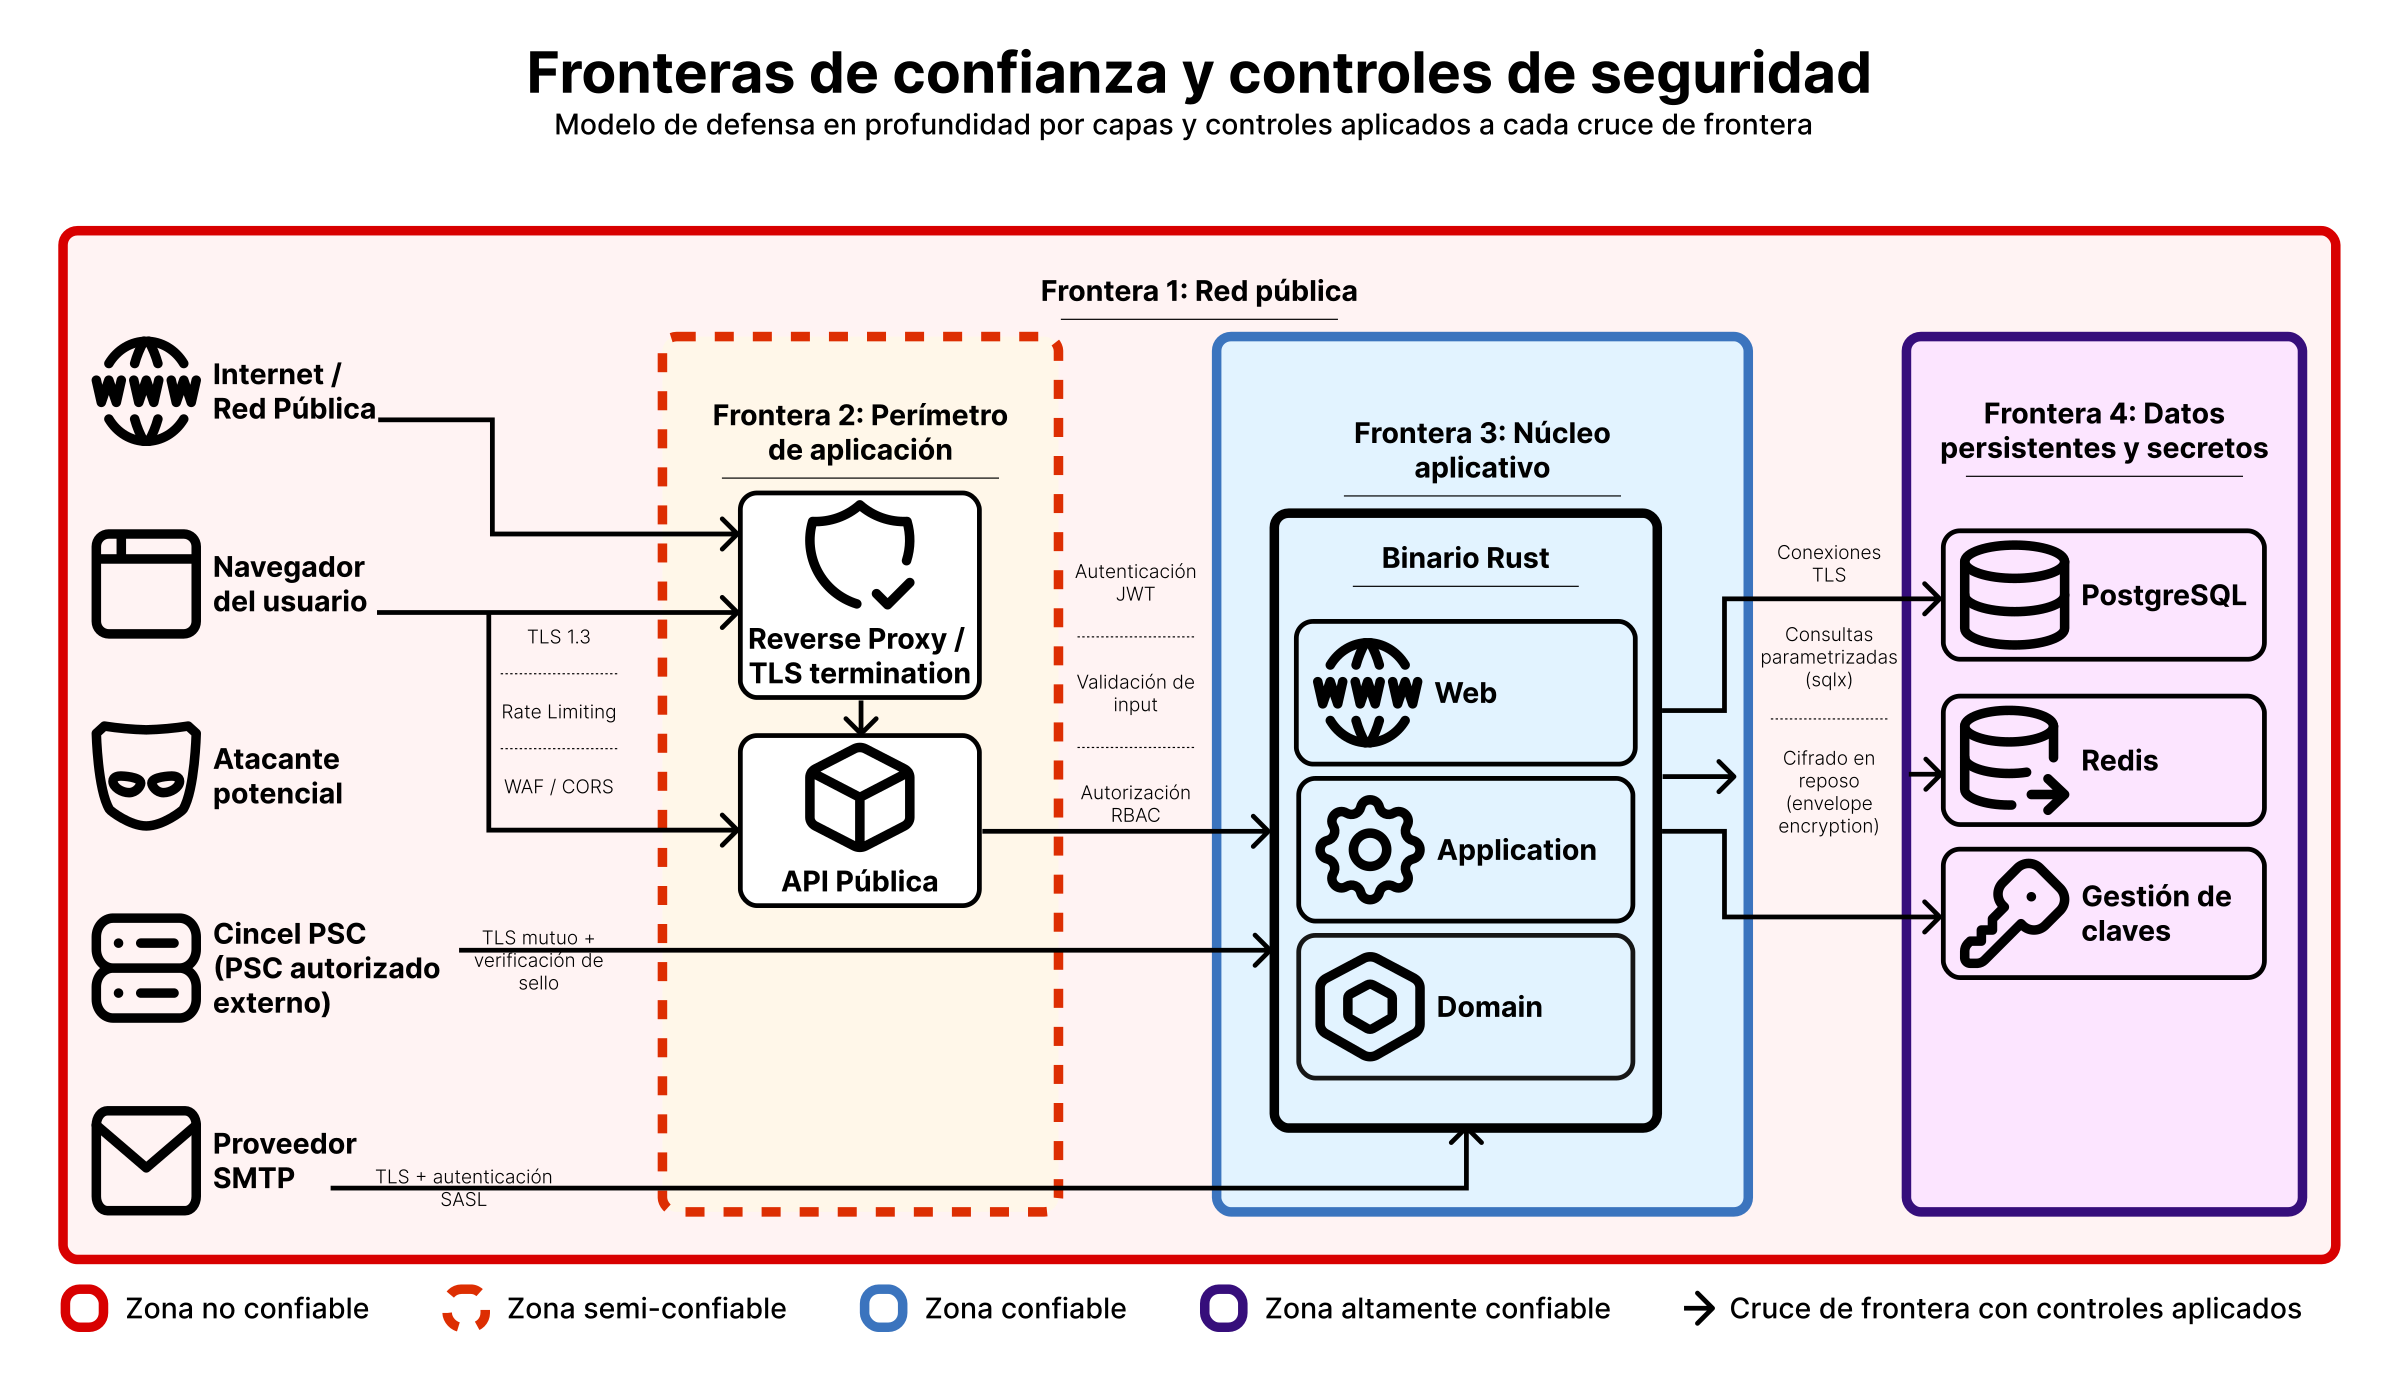
\includegraphics[width=\linewidth]{image29.png}
  \caption{Modelo de defensa en profundidad por capas y controles aplicados a cada cruce de frontera.}
  \label{fig:fronteras-confianza}
\end{figure}

\section{Arquitectura Hexagonal completa con puertos y adaptadores nombrados}\label{sec:hexagonal-completa}

Implementación detallada de la arquitectura hexagonal del prototipo: todos los puertos driving del sistema (RestApiPort sobre Axum, CommandLinePort sobre Clap, WebSocketPort sobre Axum WebSocket), todos los puertos driven (CaseRepository, DocumentRepository, DocumentSigner, TimestampService, NotificationDispatcher, AuditLogger, SessionStore) y sus adaptadores concretos correspondientes. Cada puerto se materializa como un trait de Rust en el crate domain, y cada adaptador como una struct con bloque impl en el crate infrastructure.

\begin{figure}[H]
  \centering
  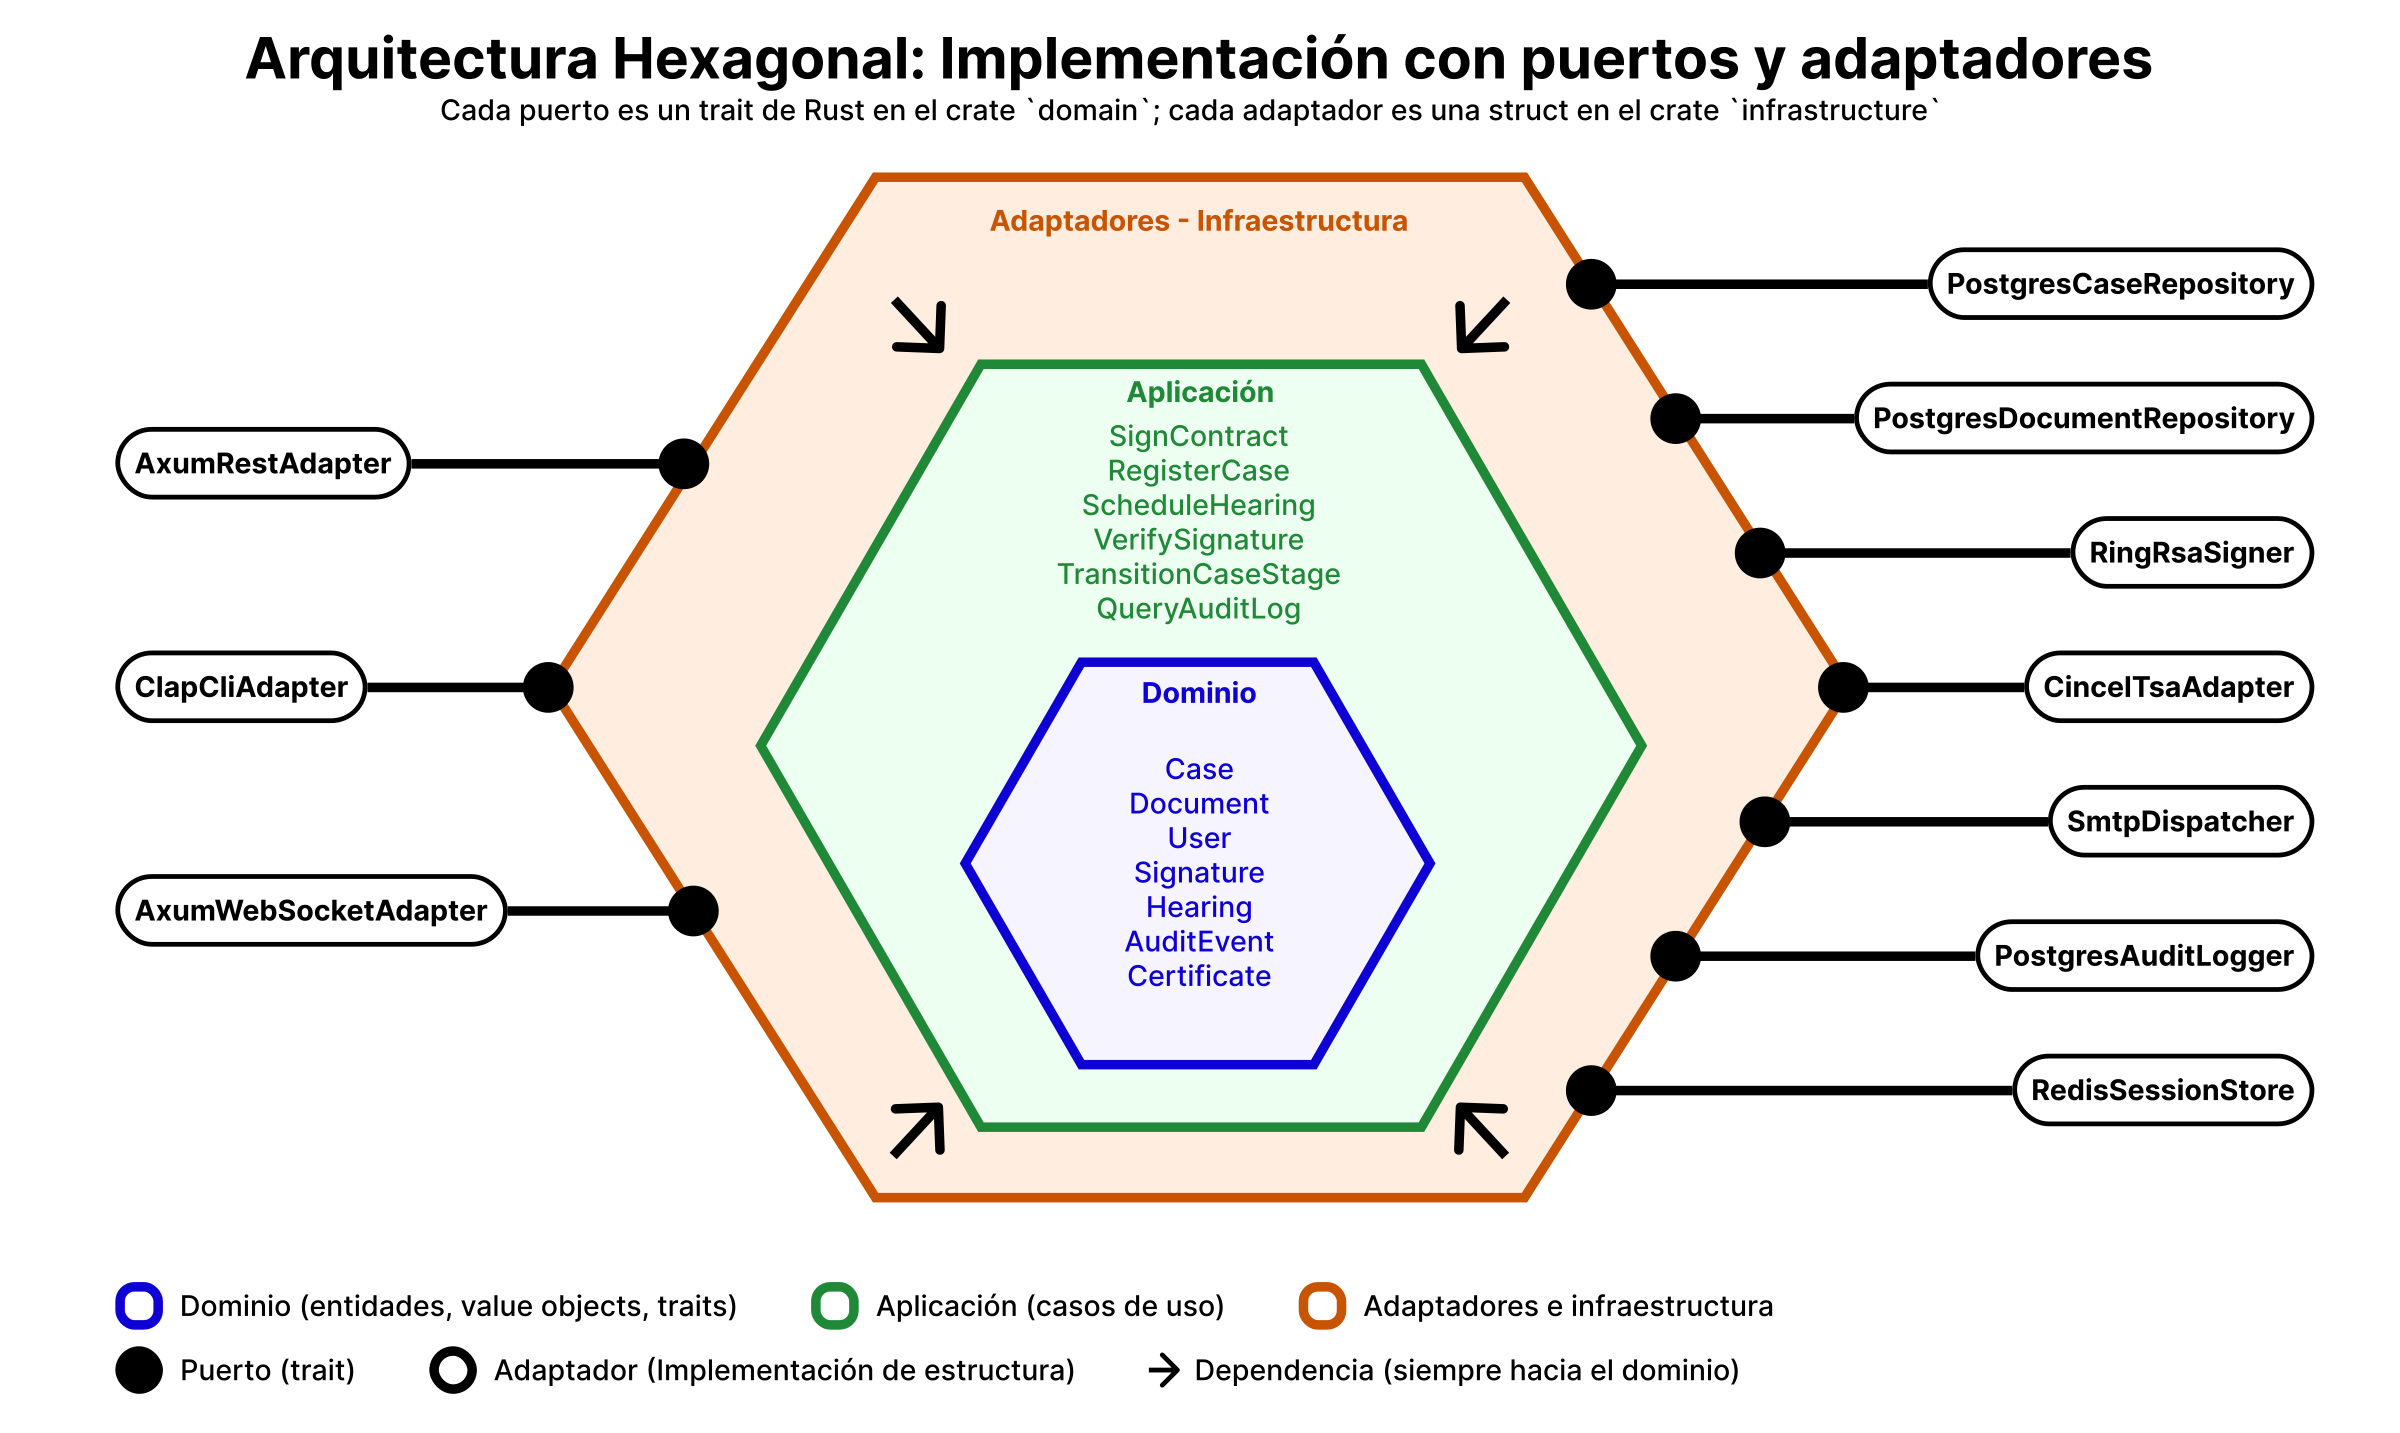
\includegraphics[width=\linewidth]{image30.png}
  \caption{Arquitectura hexagonal completa: cada puerto es un trait de Rust en el crate domain; cada adaptador es una struct en el crate infrastructure.}
  \label{fig:hexagonal-completa}
\end{figure}

% =====================================================================
%  anexo-b-cli.tex — Manual de la interfaz de línea de comandos
% =====================================================================
\chapter{Manual de la interfaz de línea de comandos}\label{anexo:cli}

Este anexo es el manual de referencia de \texttt{despacho-cli}, la interfaz de línea de comandos del prototipo. El binario lo produce el crate \texttt{bin} del workspace de Cargo, que opera como raíz de composición de la arquitectura hexagonal: los comandos componen casos de uso de aplicación y operaciones administrativas de infraestructura sin trasladar las reglas de negocio a la interfaz. El árbol de mandos está definido en \rutarepo{crates/bin/src/cli.rs}, con argumentos de servidor y base de datos en módulos separados. El contrato descrito corresponde al 12 de septiembre de 2026. Los bloques de comandos sin salida son ejemplos de uso; las transcripciones con el prefijo \texttt{+} conservan resultados históricos: provienen de la transcripción versionada \texttt{docs/demo-transcript.md}, capturada el 12 de julio de 2026 con \texttt{despacho-cli} 0.1.0 y OpenSSL 3.5.7; las mediciones de calibración se distinguen como ejemplos de su corrida y no como rendimiento actual. En esas transcripciones, \texttt{\$REPO} abrevia la raíz del repositorio y \texttt{\$WORK} el directorio temporal de trabajo de aquella ejecución.

\section{Convenciones generales}\label{sec:cli-convenciones}

El árbol completo de subcomandos es el siguiente; los corchetes denotan elementos opcionales y los ángulos, valores que aporta el usuario:

\begin{lstlisting}[numbers=none]
despacho-cli [--json]
  serve --signer-cert <PATH> --signer-key <PATH>
      [--bind <ADDR>] [--data-dir <DIR>] [--ca-cert <PATH>]
      [--crl <PATH>] [--tsa-config <PATH>] [--tsa-dir <DIR>]
      [--max-in-flight-requests <N>] [--max-blocking-operations <N>]
  database migrate --runtime-role <ROLE>
  database import [--data-dir <DIR>] --mapping <PATH> [--apply]
  crypto hash <FILE>
  vault encrypt <FILE> --doc-id <UUID> [--version <N>]
  vault decrypt <PACKAGE> --doc-id <UUID> [--version <N>] [--out <PATH>]
  vault rotate-kek --file <PATH>
  pki [--scripts-dir <DIR>] {init-ca | issue --cn <CN> |
      revoke --serial <HEX> | gen-crl | show <CERT>}
  sign <FILE> --cert <PATH> --key <PATH>
  timestamp <INPUT> [--mock] [--out <PATH>] [--pki-dir <DIR>]
  verify <FILE> --sig <PATH> --cert <PATH> --ca <PATH> [--tsr <PATH>]
      [--crl <PATH>] [--tsa-cert <PATH>] [--at <RFC3339>]
  package export <FILE> --sig <PATH> --tsr <PATH> --cert <PATH>
      --ca <PATH> --crl <PATH> [--tsa-chain <PATH>] --out <PATH>
  auth {calibrate | hash-password | verify-password --hash <PHC>}
  auth totp enroll --user <EMAIL> --secret-out <PATH>
  auth totp verify --code <CODE> --secret-file <PATH>
  audit {append --action <STRING> --resource <STRING> |
      verify-chain | show}
\end{lstlisting}

Tres convenciones gobiernan a los subcomandos administrativos. Primera, la separación de flujos: los resultados se escriben en la salida estándar (\texttt{stdout}) y los diagnósticos en el flujo de error (\texttt{stderr}), de modo que la salida pueda encadenarse en tuberías sin contaminación; el nivel de diagnóstico se controla con la variable de entorno \texttt{RUST\_LOG}. Segunda, la bandera global \texttt{--json}: cuando está activa, cada operación finita imprime un objeto JSON legible por máquina en lugar del texto para humanos; \texttt{vault decrypt} sin \texttt{--out} escribe el claro crudo y \texttt{serve} es un proceso persistente cuyo contrato se consume por HTTP. Tercera, los códigos de salida: el proceso termina con código distinto de cero ante cualquier error y también ---de forma deliberada, para que los scripts puedan bifurcar directamente--- cuando un resultado criptográfico es un rechazo: un veredicto de verificación no válido, una contraseña que no coincide, un código TOTP rechazado, una cadena de auditoría rota o un paquete de evidencia que no verifica antes de exportarse. La bandera \texttt{--help} está disponible en todos los niveles; \texttt{--version}, en el mando raíz.

El binario carga un archivo \texttt{.env} del directorio de trabajo cuando existe (nunca se versiona; la plantilla comentada es \texttt{.env.example}). La \cref{tab:cli-variables-entorno} resume las variables reconocidas; de ellas solo se registra en el diagnóstico su presencia, jamás su valor.

\begin{table}[H]
  \centering
  \caption{Variables de entorno leídas por \texttt{despacho-cli}. En las variables del proveedor remoto de sellado, un valor en blanco cuenta como ausente.}
  \label{tab:cli-variables-entorno}
  \begin{tabularx}{\linewidth}{@{}l X l@{}}
    \toprule
    \textbf{Variable} & \textbf{Propósito} & \textbf{Default} \\
    \midrule
    \texttt{RUST\_LOG} & Filtro del diagnóstico emitido por \texttt{stderr}. & \texttt{info} \\
    \texttt{KEK\_BASE64} & Llave de cifrado de llaves: 32 bytes aleatorios codificados en base64; la leen \texttt{vault}, \texttt{serve} y \texttt{database import}. & --- \\
    \texttt{NEW\_KEK\_BASE64} & Llave de reemplazo; la lee solo \texttt{vault rotate-kek}. & --- \\
    \texttt{PKI\_CA\_DIR} & Directorio de trabajo de la CA interna. & \texttt{pki-ca} \\
    \texttt{TSA\_DIR} & Directorio de trabajo de la TSA local, junto al de la CA. & \texttt{pki-tsa} \\
    \texttt{CINCEL\_BASE\_URL} & URL base del proveedor remoto de sellado de tiempo. & --- \\
    \texttt{CINCEL\_API\_KEY} & Credencial del proveedor remoto (secreto). & --- \\
    \texttt{AUDIT\_LOG\_PATH} & Archivo de bitácora offline; HTTP usa PostgreSQL. & \texttt{audit-log.jsonl} \\
    \texttt{USER} & Actor que registra \texttt{audit append}. & \texttt{unknown} \\
    \texttt{DATABASE\_URL} & Conexión PostgreSQL: administrativa en \texttt{database}, restringida en \texttt{serve}. & --- \\
    \texttt{REDIS\_URL} & Cadena Redis obligatoria para sesiones, desafíos y límites al ejecutar \texttt{serve}. & --- \\
    \bottomrule
  \end{tabularx}
\end{table}

\section{Comando serve: aplicación HTTP local}\label{sec:cli-serve}

\begin{lstlisting}[numbers=none]
despacho-cli serve --signer-cert <PATH> --signer-key <PATH>
    [--bind <ADDR>] [--data-dir <DIR>] [--ca-cert <PATH>]
    [--crl <PATH>] [--tsa-config <PATH>] [--tsa-dir <DIR>]
    [--max-in-flight-requests <N>] [--max-blocking-operations <N>]
\end{lstlisting}

El comando inicia la API de identidad, expedientes y documentos. PostgreSQL
almacena usuarios, pertenencias, contenido cifrado y auditoría; Redis conserva
sesiones, desafíos y controles de autenticación. Escucha por defecto en
\texttt{127.0.0.1:3000}. Exige \texttt{DATABASE\_URL}, \texttt{REDIS\_URL},
\texttt{KEK\_BASE64}, certificado y llave del firmante, CA, CRL y TSA local
preparada. No consulta Cincel. Los argumentos predeterminados son
\texttt{pki-ca/ca.crt.pem}, \texttt{pki-ca/crl/crl.pem}, \texttt{pki/tsa.cnf}
y \texttt{pki-tsa} para CA, CRL, configuración y directorio de TSA.

El esquema debe prepararse antes mediante \texttt{database migrate}.
\texttt{serve} no ejecuta DDL y rechaza una conexión administrativa o capaz de
reescribir los datos protegidos. \texttt{--data-dir}, cuyo valor predeterminado
es \texttt{runtime-data}, identifica el origen local preservado para comprobar
su importación; no es el destino de nuevos documentos. Si hay archivos previos,
el arranque exige marcadores de corte y reconciliación consistente con la base.

Las rutas incluyen bootstrap, login, MFA, logout, usuarios, expedientes y
asignaciones. Las operaciones documentales se ubican bajo
\texttt{/api/v1/cases/<case>/documents}; \texttt{<case>} es el UUID del expediente.
El actor procede del bearer vigente. Owner accede a todos los expedientes;
Litigante y Paralegal necesitan asignación y este último no puede sellar.
Cliente solo consulta metadatos asignados y mantiene denegado el acceso
documental. Las rutas globales anteriores bajo \texttt{/api/v1/documents}
responden \texttt{404}. El contrato se presenta en \cref{sec:impl-http}.

Los límites predeterminados son ocho peticiones admitidas y dos operaciones
bloqueantes, configurables mediante las dos opciones de concurrencia; ambas
aceptan enteros positivos. Sin capacidad, la API responde
\texttt{503 server\_busy}. Cancelar una petición no cancela automáticamente
su trabajo ni libera el permiso mientras este continúa. Aumentar los límites
requiere medir memoria y carga, especialmente por Argon2id. El servidor local
no configura por sí solo TLS ni una operación pública validada.

\section{Grupo database: esquema e importación}\label{sec:cli-database}

Estos comandos usan \texttt{DATABASE\_URL} para la base de destino.
\texttt{migrate} prepara el esquema y los permisos; \texttt{import} comprueba
y, opcionalmente, incorpora un almacenamiento local anterior. Ninguno sustituye
las operaciones autenticadas de usuarios o expedientes de la API.

\subsection{database migrate}

\begin{lstlisting}[numbers=none]
despacho-cli [--json] database migrate --runtime-role <ROLE>
\end{lstlisting}

\texttt{--runtime-role} es obligatorio y nombra un rol PostgreSQL existente.
El comando no crea su cuenta ni decide su contraseña. El operador debe preparar
la base, crear un rol de conexión sin privilegios administrativos y configurar
su autenticación. Por ejemplo, desde una sesión administrativa:

\begin{lstlisting}[numbers=none]
CREATE ROLE tt_runtime LOGIN NOSUPERUSER NOCREATEDB NOCREATEROLE;
\end{lstlisting}

Después se ejecuta la migración con una conexión administrativa; las cadenas
del ejemplo deben sustituirse por las del entorno:

\begin{lstlisting}[numbers=none]
export DATABASE_URL='postgresql://administrador@localhost/despacho'
despacho-cli database migrate --runtime-role tt_runtime
\end{lstlisting}

La preparación aplica las migraciones de identidad, expedientes, documentos y
auditoría y otorga permisos al rol indicado. Para arrancar el servidor se cambia
\texttt{DATABASE\_URL} a la conexión de \texttt{tt\_runtime}. Ese rol puede leer
y anexar auditoría, pero no actualizarla, borrarla ni truncarla. El arranque
comprueba también los privilegios sobre documentos, recibos y la protección
de evidencia; los propietarios y administradores siguen formando parte de
la base de confianza. Con \texttt{--json}, la salida de \texttt{migrate}
contiene \texttt{migrated} y \texttt{runtime\_role}.

\subsection{database import}

\begin{lstlisting}[numbers=none]
despacho-cli [--json] database import [--data-dir <DIR>]
    --mapping <PATH> [--apply]
\end{lstlisting}

\texttt{--data-dir} identifica el origen, con valor predeterminado
\texttt{runtime-data}; \texttt{--mapping} es obligatorio. El modo predeterminado
inspecciona fuentes y destino sin escribir archivos ni datos. Solo
\texttt{--apply} confirma la importación. Se requiere la KEK original en
\texttt{KEK\_BASE64}; generar una nueva no recupera los documentos anteriores.
La validación no necesita la llave privada del firmante ni solicitar un sello.

Antes de proceder deben detenerse todos los escritores, incluidas versiones
antiguas del servidor y comandos \texttt{audit append} que apunten al mismo
origen. Debe respaldarse la base existente y conservarse una copia de fuentes,
KEK y material criptográfico. La base de destino debe tener el esquema preparado
y los expedientes ya existentes. En la primera importación, sus tablas de
documentos y auditoría deben estar vacías para conservar la cadena histórica
como prefijo; no se antepone historia a eventos nuevos.

El mapa es un JSON explícito con una entrada por documento. Los UUID del ejemplo
son ilustrativos y deben corresponder a archivos y expedientes reales:

\begin{lstlisting}[numbers=none]
{
  "documents": [
    {
      "document_id": "11111111-1111-4111-8111-111111111111",
      "case_id": "22222222-2222-4222-8222-222222222222"
    }
  ]
}
\end{lstlisting}

La inspección rechaza asociaciones ausentes, duplicados, archivos inesperados,
identidades inconsistentes, digest o contexto de cifrado alterados y bitácoras
rotas o con referencias documentales huérfanas. Comprueba firma y sello; evalúa
la cadena y CRL del firmante en la fecha autenticada del sello. La confianza
TSA conserva la política actual de OpenSSL: una TSA expirada hoy puede impedir
la importación histórica. Un rechazo exige preservar el origen y revisar la
causa, sin sustituir ni regenerar la evidencia para forzar aceptación.

Con las fuentes detenidas y la conexión administrativa seleccionada, se ejecuta
primero la inspección y se revisan los conteos, huella de fuentes y cabeza de
auditoría. La misma orden con \texttt{--apply} confirma:

\begin{lstlisting}[numbers=none]
despacho-cli --json database import \
  --data-dir /ruta/runtime-data --mapping /ruta/mapping.json

despacho-cli --json database import \
  --data-dir /ruta/runtime-data --mapping /ruta/mapping.json --apply
\end{lstlisting}

La transacción conserva ciphertext, evidencia y hashes históricos, añade el
evento de importación y guarda un recibo. La salida JSON contiene
\texttt{applied} y \texttt{report}; el reporte incluye huella, conteos,
cabeza histórica y hashes de los archivos. \texttt{audit\_entries} cuenta
las entradas originales, sin incluir el evento nuevo de importación.

Antes de insertar se instalan barreras \texttt{.migration-pending} que mantienen
bloqueados ambos almacenes de archivos si ocurre un fallo. Tras el commit se
instalan marcadores \texttt{.migrated} y se retiran las barreras. Un fallo
posterior al commit se informa como importación confirmada con corte pendiente:
se corrige la causa de archivos y se repiten las mismas fuentes y mapa. La
repetición reconcilia el contenido y el recibo, completa marcadores faltantes
y no duplica documentos ni eventos. No deben borrarse las barreras para reabrir
un origen de estado incierto. Los ejecutables antiguos no las reconocen y deben
permanecer detenidos.

Finalmente se inicia \texttt{serve} con el rol operativo y
\texttt{--data-dir} apuntando al origen preservado. El arranque verifica
marcadores, recibo, asociaciones, documentos y cadena completa. Deben comprobarse
accesos y exportaciones antes de habilitar tráfico. Restaurar requiere PostgreSQL
completo, permisos y KEK protegida por separado; un recibo aislado o una copia
documental parcial no bastan. Las sesiones Redis previas deben invalidarse en
una recuperación operativa. El procedimiento versionado y su ensayo desechable
se describen en \rutarepo{docs/database-operations.md}.

\section{Grupo crypto: integridad de contenido}\label{sec:cli-crypto}

\subsection{crypto hash}

\begin{lstlisting}[numbers=none]
despacho-cli [--json] crypto hash <FILE>
\end{lstlisting}

Calcula el resumen SHA-256 del archivo indicado y lo imprime en hexadecimal en minúsculas. El único argumento, \texttt{<FILE>} (posicional, ruta, obligatorio), se consume como flujo en bloques de 64 KiB, por lo que el uso de memoria es constante sin importar el tamaño de la entrada. Un archivo inexistente termina el proceso con código distinto de cero.

\begin{lstlisting}[numbers=none]
+ $REPO/target/debug/despacho-cli crypto hash document.txt
fb5c0a6097be9246860fa82c89db3576e8a4ba7e554f3954f148f8bdfdd27ad9
\end{lstlisting}

Con \texttt{--json}, la salida es un objeto con los campos \texttt{algorithm} (siempre \texttt{"sha-256"}), \texttt{digest} y \texttt{file}.

\section{Grupo vault: cifrado en reposo}\label{sec:cli-vault}

Los tres subcomandos de \texttt{vault} materializan el cifrado autenticado en reposo con AES-256-GCM y envelope encryption: cada documento se cifra con una llave de datos (DEK) fresca, que a su vez se almacena envuelta bajo la llave de cifrado de llaves (KEK) leída de la variable \texttt{KEK\_BASE64}. El criptograma queda ligado a la identidad y versión del documento mediante los datos adicionales autenticados (AAD), de modo que descifrar con un identificador o versión distintos falla igual que un criptograma alterado. La \cref{tab:cli-vault-opciones} lista las opciones.

\begin{table}[H]
  \centering
  \caption{Opciones de los subcomandos del grupo \texttt{vault}.}
  \label{tab:cli-vault-opciones}
  \begin{tabularx}{\linewidth}{@{}l l l X@{}}
    \toprule
    \textbf{Opción} & \textbf{Tipo} & \textbf{Default} & \textbf{Descripción} \\
    \midrule
    \multicolumn{4}{@{}l}{\textbf{vault encrypt}} \\
    \texttt{<FILE>} & ruta & obligatorio & Archivo en claro; el resultado se escribe en \texttt{<FILE>.enc}. \\
    \texttt{--doc-id} & cadena (UUID) & obligatorio & Identidad del documento a la que se liga el criptograma. \\
    \texttt{--version} & entero & \texttt{1} & Versión del documento ligada al criptograma. \\
    \midrule
    \multicolumn{4}{@{}l}{\textbf{vault decrypt}} \\
    \texttt{<PACKAGE>} & ruta & obligatorio & Paquete cifrado producido por \texttt{encrypt}. \\
    \texttt{--doc-id} & cadena (UUID) & obligatorio & Identidad esperada dentro del paquete. \\
    \texttt{--version} & entero & \texttt{1} & Versión esperada dentro del paquete. \\
    \texttt{--out} & ruta & \texttt{stdout} & Destino del texto claro. \\
    \midrule
    \multicolumn{4}{@{}l}{\textbf{vault rotate-kek}} \\
    \texttt{--file} & ruta & obligatorio & Paquete cuya DEK se re-envuelve in situ. \\
    \bottomrule
  \end{tabularx}
\end{table}

\texttt{vault rotate-kek} lee la KEK vigente de \texttt{KEK\_BASE64} y su reemplazo de \texttt{NEW\_KEK\_BASE64}, re-envuelve únicamente la llave de datos y copia intactos los bytes del documento sellado, por lo que su costo criptográfico es independiente del tamaño del documento (la E/S de copiar el paquete sí crece con él); la escritura ocurre sobre un archivo temporal que después se renombra, de modo que un fallo a la mitad deja el original intacto. El ejemplo siguiente muestra el ciclo con detección de alteraciones: se cifra el documento, se corrompe un byte del paquete, el descifrado se rechaza con el error opaco de autenticación, se restaura el byte y se rota la KEK.

\begin{lstlisting}[numbers=none]
+ $REPO/target/debug/despacho-cli vault encrypt document.txt --doc-id 00000000-0000-4000-8000-000000000001 --version 1
wrote document.txt.enc
+ $REPO/scripts/flip-byte.sh document.txt.enc 512
flipped byte at offset 512 of document.txt.enc: 0x45 -> 0xba (size 3678 bytes, unchanged)
+ (expected to fail) $REPO/target/debug/despacho-cli vault decrypt document.txt.enc --doc-id 00000000-0000-4000-8000-000000000001 --out rechazado.txt
Error: decryption of document.txt.enc failed

Caused by:
    authenticated decryption failed
+ $REPO/scripts/flip-byte.sh document.txt.enc 512
flipped byte at offset 512 of document.txt.enc: 0xba -> 0x45 (size 3678 bytes, unchanged)
+ $REPO/target/debug/despacho-cli vault rotate-kek --file document.txt.enc
rewrapped the data key in document.txt.enc
\end{lstlisting}

Con \texttt{--json}: \texttt{encrypt} emite \texttt{package\_path}; \texttt{decrypt} con \texttt{--out} emite \texttt{out}; \texttt{rotate-kek} emite \texttt{rewritten}. \texttt{decrypt} sin \texttt{--out} escribe el texto claro crudo a \texttt{stdout} incluso bajo \texttt{--json}.

\section{Grupo pki: autoridad certificadora interna}\label{sec:cli-pki}

El grupo \texttt{pki} administra la autoridad certificadora interna ejecutando como subprocesos los scripts versionados del directorio \texttt{pki/} (detallados en el Anexo~\ref{anexo:pki}). La opción de grupo \texttt{--scripts-dir} (ruta, default \texttt{pki}) indica dónde viven los scripts; el directorio de trabajo de la CA se toma de \texttt{PKI\_CA\_DIR} (default \texttt{pki-ca} bajo el directorio actual). La \cref{tab:cli-pki-opciones} lista las opciones.

\begin{table}[H]
  \centering
  \caption{Opciones de los subcomandos del grupo \texttt{pki}.}
  \label{tab:cli-pki-opciones}
  \begin{tabularx}{\linewidth}{@{}l l l X@{}}
    \toprule
    \textbf{Opción} & \textbf{Tipo} & \textbf{Default} & \textbf{Descripción} \\
    \midrule
    \texttt{--scripts-dir} & ruta & \texttt{pki} & Directorio con los scripts de la autoridad (opción del grupo). \\
    \midrule
    \multicolumn{4}{@{}l}{\textbf{pki init-ca} (sin opciones propias)} \\
    \midrule
    \multicolumn{4}{@{}l}{\textbf{pki issue}} \\
    \texttt{--cn} & cadena & obligatorio & Common name del sujeto del certificado. \\
    \midrule
    \multicolumn{4}{@{}l}{\textbf{pki revoke}} \\
    \texttt{--serial} & cadena (hex) & obligatorio & Serial del certificado, tal como lo imprimen \texttt{issue} y \texttt{show}. \\
    \midrule
    \multicolumn{4}{@{}l}{\textbf{pki gen-crl} (sin opciones propias)} \\
    \midrule
    \multicolumn{4}{@{}l}{\textbf{pki show}} \\
    \texttt{<CERT>} & ruta & obligatorio & Certificado a inspeccionar. \\
    \bottomrule
  \end{tabularx}
\end{table}

\texttt{init-ca} crea la raíz autofirmada y es idempotente: re-ejecutarlo sobre una CA existente no la reemplaza. \texttt{issue} emite un certificado de entidad final y rehúsa reportar éxito hasta validar el certificado fresco contra la raíz. \texttt{revoke} marca el serial en la base de datos de la CA; la revocación solo se vuelve visible para terceros tras regenerar la lista con \texttt{gen-crl}. \texttt{show} imprime sujeto, emisor, serial y ventana de vigencia de cualquier certificado.

\begin{lstlisting}[numbers=none]
+ $REPO/target/debug/despacho-cli pki --scripts-dir $REPO/pki init-ca
certificate authority ready at $WORK/pki-ca
root certificate: $WORK/pki-ca/ca.crt.pem
+ $REPO/target/debug/despacho-cli pki --scripts-dir $REPO/pki issue --cn "Socia Demo"
issued certificate serial 1000
  certificate: $WORK/pki-ca/certs/socia-demo.crt.pem
  private key: $WORK/pki-ca/private/socia-demo.key.pem (keep secret, never commit)
+ $REPO/target/debug/despacho-cli pki --scripts-dir $REPO/pki revoke --serial 1000
revoked certificate serial 1000
run 'pki gen-crl' to publish an updated revocation list
+ $REPO/target/debug/despacho-cli pki --scripts-dir $REPO/pki gen-crl
wrote $WORK/pki-ca/crl/crl.pem
\end{lstlisting}

Con la bandera \texttt{--json}: \texttt{init-ca} emite \texttt{ca\_dir} y \texttt{root\_certificate}; \texttt{issue} emite \texttt{serial}, \texttt{certificate} y \texttt{private\_key}; \texttt{revoke} emite \texttt{revoked\_serial}; \texttt{gen-crl} emite \texttt{crl}; \texttt{show} emite \texttt{subject}, \texttt{issuer}, \texttt{serial}, \texttt{not\_before} y \texttt{not\_after}.

\section{Comando sign: firma digital}\label{sec:cli-sign}

\begin{lstlisting}[numbers=none]
despacho-cli [--json] sign <FILE> --cert <PATH> --key <PATH>
\end{lstlisting}

Firma el resumen SHA-256 del documento con RSA PKCS\#1 v1.5 y escribe la firma separada en \texttt{<FILE>.sig}. \texttt{<FILE>} (posicional, ruta) es el documento a firmar; \texttt{--cert} (ruta, obligatoria) es el certificado del firmante y \texttt{--key} (ruta, obligatoria) su llave privada en PEM, en codificación PKCS\#8 o PKCS\#1; llaves con módulo menor a 3\,072 bits se rechazan al construir el firmador. Antes de escribir el archivo de firma, el comando verifica la firma recién producida contra el certificado presentado: una llave que no corresponde al certificado falla en ese punto en lugar de producir una firma inverificable.

\begin{lstlisting}[numbers=none]
+ $REPO/target/debug/despacho-cli sign document.txt --cert $WORK/pki-ca/certs/socia-demo.crt.pem --key $WORK/pki-ca/private/socia-demo.key.pem
digest: fb5c0a6097be9246860fa82c89db3576e8a4ba7e554f3954f148f8bdfdd27ad9
signature: document.txt.sig
\end{lstlisting}

Con \texttt{--json}, la salida contiene \texttt{digest}, \texttt{signature\_path} y \texttt{certificate\_subject}.

\section{Comando timestamp: sellado de tiempo}\label{sec:cli-timestamp}

\begin{lstlisting}[numbers=none]
despacho-cli [--json] timestamp <INPUT> [--mock] [--out <PATH>]
    [--pki-dir <DIR>]
\end{lstlisting}

Solicita un sello de tiempo RFC 3161 sobre el resumen SHA-256 del archivo \texttt{<INPUT>} (posicional, ruta) y escribe el token DER en \texttt{<INPUT>.tsr}, o en la ruta dada con \texttt{--out}. Con la bandera \texttt{--mock} (booleana), la autoridad es la TSA local de OpenSSL: su directorio de trabajo se lee de \texttt{TSA\_DIR} (default \texttt{pki-tsa}, junto al directorio de la CA) y la configuración \texttt{tsa.cnf} se busca en \texttt{--pki-dir} (ruta, default \texttt{pki}). Sin \texttt{--mock}, se usa el proveedor remoto: el comando exige \texttt{CINCEL\_BASE\_URL} y \texttt{CINCEL\_API\_KEY} no vacías en el entorno, con tiempo límite de 15 segundos por solicitud y hasta cinco sondeos cada dos segundos cuando el proveedor difiere la emisión; si faltan, aborta indicando que se configuren esas variables o se use \texttt{--mock}. En ambos casos, tras obtener el token el comando lo relee y exige que cubra exactamente el resumen calculado antes de escribir archivo alguno: una autoridad que respondiera con un token inutilizable falla aquí sin dejar un archivo espurio.

\begin{lstlisting}[numbers=none]
+ $REPO/target/debug/despacho-cli timestamp document.txt --mock --pki-dir $REPO/pki
digest: fb5c0a6097be9246860fa82c89db3576e8a4ba7e554f3954f148f8bdfdd27ad9
token: document.txt.tsr
generated at: 2026-07-12T10:19:41Z
\end{lstlisting}

Con \texttt{--json}, la salida contiene \texttt{digest}, \texttt{token\_path} y \texttt{generated\_at}.

\section{Comando verify: verificación integral}\label{sec:cli-verify}

\begin{lstlisting}[numbers=none]
despacho-cli [--json] verify <FILE> --sig <PATH> --cert <PATH>
    --ca <PATH> [--tsr <PATH>] [--crl <PATH>] [--tsa-cert <PATH>]
    [--at <RFC3339>]
\end{lstlisting}

Produce un reporte de cuatro componentes sobre el documento: integridad (el resumen recomputado contra el que atestigua el token de sello), firma, estado del certificado del firmante y sello de tiempo. La \cref{tab:cli-verify-opciones} lista las opciones.

\begin{table}[H]
  \centering
  \caption{Opciones del comando \texttt{verify}.}
  \label{tab:cli-verify-opciones}
  \begin{tabularx}{\linewidth}{@{}l l l X@{}}
    \toprule
    \textbf{Opción} & \textbf{Tipo} & \textbf{Default} & \textbf{Descripción} \\
    \midrule
    \texttt{<FILE>} & ruta & obligatorio & Documento original. \\
    \texttt{--sig} & ruta & obligatorio & Firma separada. \\
    \texttt{--cert} & ruta & obligatorio & Certificado del firmante. \\
    \texttt{--ca} & ruta & obligatorio & Certificado de la autoridad emisora. \\
    \texttt{--tsr} & ruta & --- & Token de sello de tiempo; sin él, los componentes que dependen del token se reportan omitidos con su razón. \\
    \texttt{--crl} & ruta & --- & Lista de revocación; sin ella no se comprueba revocación y el reporte lo dice. \\
    \texttt{--tsa-cert} & ruta & \texttt{--ca} & Ancla de confianza para el token; por defecto el propio emisor, que ancla a las autoridades internas. \\
    \texttt{--at} & instante RFC 3339 & ahora & Instante de evaluación del estado del certificado. \\
    \bottomrule
  \end{tabularx}
\end{table}

La semántica del veredicto es estricta: un componente cuya evidencia no se aportó se reporta omitido (\texttt{skipped}) con su razón y no cuenta contra el veredicto; el veredicto es \texttt{not valid} si cualquier componente ejercitado falló, y en ese caso el proceso termina con código distinto de cero. El estado del certificado habla únicamente del instante de evaluación: el propio reporte aclara que un certificado hoy expirado o revocado no invalida por sí mismo una firma efectuada mientras era válido, lectura que corresponde a quien valora la evidencia. El primer ejemplo muestra una verificación íntegra; el segundo, la misma evidencia después de revocar el certificado y regenerar la CRL.

\begin{lstlisting}[numbers=none]
+ $REPO/target/debug/despacho-cli verify document.txt --sig document.txt.sig --tsr document.txt.tsr --cert $WORK/pki-ca/certs/socia-demo.crt.pem --ca $WORK/pki-ca/ca.crt.pem --crl $WORK/pki-ca/crl/crl.pem
document:    document.txt
digest:      fb5c0a6097be9246860fa82c89db3576e8a4ba7e554f3954f148f8bdfdd27ad9
integrity:   passed: recomputed digest matches the digest the timestamp token attests
signature:   passed: signature verifies over the document digest with the signer certificate
certificate: passed: status at the evaluation time: valid (revocation checked against the supplied list)
timestamp:   passed: token accepted under the trust anchor; generated at 2026-07-12T10:19:41Z
verdict:     valid
\end{lstlisting}

\begin{lstlisting}[numbers=none]
+ (expected to fail) $REPO/target/debug/despacho-cli verify document.txt --sig document.txt.sig --tsr document.txt.tsr --cert $WORK/pki-ca/certs/socia-demo.crt.pem --ca $WORK/pki-ca/ca.crt.pem --crl $WORK/pki-ca/crl/crl.pem
document:    document.txt
digest:      fb5c0a6097be9246860fa82c89db3576e8a4ba7e554f3954f148f8bdfdd27ad9
integrity:   passed: recomputed digest matches the digest the timestamp token attests
signature:   passed: signature verifies over the document digest with the signer certificate
certificate: failed: status at the evaluation time: revoked (serial 1000); this status speaks for the evaluation time only and does not by itself invalidate a signature made while the certificate was valid
timestamp:   passed: token accepted under the trust anchor; generated at 2026-07-12T10:19:41Z
verdict:     not valid
Error: the verification verdict is not valid
\end{lstlisting}

Con \texttt{--json}, la salida contiene \texttt{document}, \texttt{digest}, un objeto \texttt{\{status, detail\}} por cada uno de los componentes \texttt{integrity}, \texttt{signature}, \texttt{certificate} y \texttt{timestamp}, y el campo \texttt{verdict}.

\section{Grupo package: paquete de evidencia}\label{sec:cli-package}

\begin{lstlisting}[numbers=none]
despacho-cli [--json] package export <FILE> --sig <PATH> --tsr <PATH>
    --cert <PATH> --ca <PATH> --crl <PATH> [--tsa-chain <PATH>]
    --out <PATH>
\end{lstlisting}

Construye el paquete de evidencia autocontenido: un archivo ZIP con el documento, su firma, su sello de tiempo, los certificados, la lista de revocación y el instructivo \texttt{INSTRUCCIONES.md} de verificación independiente (la guía completa se reproduce en el Anexo~\ref{anexo:verificacion}). Todas las opciones son rutas obligatorias salvo \texttt{--tsa-chain} (ruta, opcional), que incluye la cadena de certificados de la autoridad de sellado cuando está disponible; si viaja, las instrucciones anclan la comprobación del token en esa cadena, y si no, en el certificado del emisor. Antes de escribir el ZIP, el comando ejecuta la misma verificación integral de \texttt{verify} sobre los artefactos, incluidos CRL y token, y rehúsa exportar si el veredicto no es válido, nombrando cada componente fallido: el paquete nunca puede fallar sus propias instrucciones.

\begin{lstlisting}[numbers=none]
+ $REPO/target/debug/despacho-cli package export document.txt --sig document.txt.sig --tsr document.txt.tsr --cert $WORK/pki-ca/certs/socia-demo.crt.pem --ca $WORK/pki-ca/ca.crt.pem --crl $WORK/pki-ca/crl/crl.pem --tsa-chain $WORK/pki-tsa/tsa-chain.pem --out evidencia.zip
digest:  fb5c0a6097be9246860fa82c89db3576e8a4ba7e554f3954f148f8bdfdd27ad9
package: evidencia.zip
instructions inside the package: INSTRUCCIONES.md
\end{lstlisting}

Con \texttt{--json}, la salida contiene \texttt{digest}, \texttt{package} e \texttt{instructions}.

\section{Grupo auth: credenciales y segundo factor}\label{sec:cli-auth}

El grupo \texttt{auth} cubre el hashing de contraseñas con Argon2id, su calibración empírica y el segundo factor TOTP con códigos de recuperación. Las contraseñas nunca viajan como argumentos: se leen de la entrada estándar hacia búferes que se borran de memoria al liberarse. La \cref{tab:cli-auth-opciones} lista las opciones.

\begin{table}[H]
  \centering
  \caption{Opciones de los subcomandos del grupo \texttt{auth}.}
  \label{tab:cli-auth-opciones}
  \begin{tabularx}{\linewidth}{@{}l l l X@{}}
    \toprule
    \textbf{Opción} & \textbf{Tipo} & \textbf{Default} & \textbf{Descripción} \\
    \midrule
    \multicolumn{4}{@{}l}{\textbf{auth calibrate} (sin opciones; no lee contraseña)} \\
    \midrule
    \multicolumn{4}{@{}l}{\textbf{auth hash-password} (contraseña por \texttt{stdin})} \\
    \midrule
    \multicolumn{4}{@{}l}{\textbf{auth verify-password} (contraseña por \texttt{stdin})} \\
    \texttt{--hash} & cadena (PHC) & obligatorio & Hash almacenado contra el que se verifica. \\
    \midrule
    \multicolumn{4}{@{}l}{\textbf{auth totp enroll}} \\
    \texttt{--user} & cadena (correo) & obligatorio & Identificador de la cuenta que se inscribe. \\
    \texttt{--secret-out} & ruta & obligatorio & Archivo que recibe el secreto base32 (modo 0600). \\
    \midrule
    \multicolumn{4}{@{}l}{\textbf{auth totp verify}} \\
    \texttt{--code} & cadena & obligatorio & Código de un solo uso a verificar. \\
    \texttt{--secret-file} & ruta & obligatorio & Archivo con el secreto base32 escrito al inscribir. \\
    \bottomrule
  \end{tabularx}
\end{table}

\texttt{calibrate} mide el costo real del hash en el hardware local: ejecuta cinco corridas de Argon2id sobre una muestra fija y clasifica la media contra la banda objetivo inclusiva de 500 a 1\,000 milisegundos, con veredicto por debajo, dentro o por encima de la banda. La configuración vigente es $m=262144$, $t=2$, $p=1$; la media debe medirse en cada entorno. El valor del ejemplo corresponde a una corrida anterior y no constituye una medición actual. \texttt{hash-password} emite la cadena PHC resultante, que registra esos parámetros (\texttt{\$argon2id\$v=19\$m=262144,t=2,p=1\$\ldots}). \texttt{verify-password} responde \texttt{match} o \texttt{mismatch} ---con código de salida distinto de cero en el segundo caso---, y un hash almacenado ilegible es un error, nunca un \texttt{mismatch}. \texttt{totp enroll} genera el secreto compartido, imprime el URI de aprovisionamiento \texttt{otpauth} y los ocho códigos de recuperación de un solo uso, y escribe el secreto base32 en el archivo indicado. \texttt{totp verify} acepta un desfase de un paso de 30 segundos a cada lado; la CLI conserva verificación sin estado, mientras la API rechaza la reutilización mediante un reclamo atómico en Redis.

\begin{lstlisting}[numbers=none]
+ $REPO/target/debug/despacho-cli auth calibrate
mean over 5 runs: 529.4 ms (inside the 500-1000 ms target band)
+ $REPO/target/debug/despacho-cli auth totp enroll --user demo@example.com --secret-out totp-secret.b32
otpauth-uri: otpauth://totp/despacho:demo%40example.com?secret=IGAPAF2O2XDMIG6QGFZU2YITPDCD44P3&issuer=despacho
secret-base32: IGAPAF2O2XDMIG6QGFZU2YITPDCD44P3
recovery codes (each works exactly once):
  GQVMH-DCWJS
  9QBY1-NXNJ3
  MY4P3-CX4HZ
  0CE8T-KBNSS
  31D0P-GDAD8
  B6B6N-DBGAJ
  ZV2T3-B35JJ
  C329Q-TTBEE
secret written to totp-secret.b32
+ despacho-cli auth totp verify --code (computed with openssl)
accepted
\end{lstlisting}

Con \texttt{--json}: \texttt{calibrate} emite \texttt{runs}, \texttt{mean\_ms}, \texttt{band\_min\_ms}, \texttt{band\_max\_ms} y \texttt{verdict}; \texttt{hash-password} emite \texttt{phc}; \texttt{verify-password} emite \texttt{match}; \texttt{totp enroll} emite \texttt{otpauth\_uri}, \texttt{secret\_base32}, el arreglo \texttt{recovery\_codes} y \texttt{secret\_path}; \texttt{totp verify} emite \texttt{accepted}.

\section{Grupo audit: bitácora encadenada}\label{sec:cli-audit}

El grupo \texttt{audit} opera la bitácora offline de solo anexado, separada de la cadena PostgreSQL del servidor: un archivo JSON Lines cuya ruta se toma de \texttt{AUDIT\_LOG\_PATH}, donde cada entrada almacena, además de sus campos, un valor de cadena SHA-256 que la enlaza con la anterior desde un génesis fijo. \texttt{append} registra un evento con las opciones \texttt{--action} y \texttt{--resource} (cadenas, obligatorias); el actor se toma de la variable \texttt{USER} y el instante del reloj del sistema, e imprime la secuencia y el valor de cadena asignados, de modo que la terminal del operador retenga un registro informal de la cabeza de la cadena. \texttt{verify-chain} recomputa cada eslabón desde el génesis y nombra el índice del primer eslabón roto; \texttt{show} lista las entradas en orden de inserción. Los subcomandos de lectura rehúsan operar sobre una bitácora inexistente ---reportar una ruta equivocada o un archivo borrado como cadena vacía válida frustraría la verificación---; solo \texttt{append} crea el archivo. La verificación no detecta el truncado de la cola, limitación documentada en \texttt{docs/adr/0007-audit-chain-anchoring.md}.

El actor \texttt{USER} de esta herramienta offline no autentica una identidad
HTTP. Para comprobar la cadena del servidor se usa la ruta protegida
\texttt{GET /api/v1/audit/verify} como Owner. \texttt{audit append} rechaza
un origen marcado como migrado o pendiente de migración; no se debe utilizar
un ejecutable anterior para eludir ese corte.

\begin{lstlisting}[numbers=none]
+ $REPO/target/debug/despacho-cli audit append --action demo.firma --resource document.txt.sig
appended entry 0 with chain e8b3fefc3966e47a695260f2b098dd73eff0f7da9e9b4692314df873b1e083fa
+ $REPO/target/debug/despacho-cli audit append --action demo.sello --resource document.txt.tsr
appended entry 1 with chain ffc1a151ecc7e5976d24b0bbfaaaed4c9230a8ed597938e24e6c228b2a0a5581
+ $REPO/target/debug/despacho-cli audit verify-chain
audit chain valid (2 entries)
+ $REPO/target/debug/despacho-cli audit show
0 2026-07-12T10:19:42.272903635Z eddndev demo.firma document.txt.sig e8b3fefc3966e47a695260f2b098dd73eff0f7da9e9b4692314df873b1e083fa
1 2026-07-12T10:19:42.275499975Z eddndev demo.sello document.txt.tsr ffc1a151ecc7e5976d24b0bbfaaaed4c9230a8ed597938e24e6c228b2a0a5581
+ sed -i s/demo.sello/demo.XXXXX/ $WORK/audit-log.jsonl
+ (expected to fail) $REPO/target/debug/despacho-cli audit verify-chain
Error: audit chain broken at index 1
\end{lstlisting}

Con \texttt{--json}: \texttt{append} emite \texttt{sequence}, \texttt{timestamp}, \texttt{actor}, \texttt{action}, \texttt{resource} y \texttt{chain}; \texttt{show} emite un arreglo de objetos con esos mismos campos; \texttt{verify-chain} emite \texttt{\{valid, entries\}} cuando la cadena es válida o \texttt{\{valid: false, first\_broken\_index\}} ---impreso antes de terminar con código distinto de cero--- cuando está rota.

% =====================================================================
%  anexo-c-verificacion.tex — Guía de verificación independiente
% =====================================================================
\chapter[Guía de verificación independiente con OpenSSL]{Guía de verificación independiente\\ con OpenSSL}\label{anexo:verificacion}

Cada paquete de evidencia exportado por el prototipo (comando \texttt{package export}, véase el Anexo~\ref{anexo:cli}) viaja con un instructivo \texttt{INSTRUCCIONES.md} que permite a un tercero ---un perito, la contraparte procesal o un tribunal--- verificar el documento, su firma, el estado del certificado y el sello de tiempo usando únicamente la herramienta de línea de comandos \texttt{openssl}, sin el software que generó el paquete. El instructivo se genera a partir de la plantilla versionada \texttt{crates/application/src/evidence/\allowbreak INSTRUCCIONES.template.md}, cuyos marcadores se rellenan al momento de exportar con los datos concretos del paquete (\cref{tab:verificacion-marcadores}). Este anexo reproduce esa guía paso a paso y explica qué demuestra cada comando; con ello se materializa el criterio de verificabilidad independiente del objetivo OE-3. Las salidas mostradas provienen de la ejecución real registrada en \texttt{docs/demo-transcript.md}.

\begin{table}[H]
  \centering
  \caption{Marcadores de la plantilla del instructivo y valor con que se rellenan al exportar.}
  \label{tab:verificacion-marcadores}
  \begin{tabularx}{\linewidth}{@{}l X@{}}
    \toprule
    \textbf{Marcador} & \textbf{Valor al exportar} \\
    \midrule
    \texttt{\{\{DOCUMENTO\}\}} & Nombre base del documento original. \\
    \texttt{\{\{FIRMA\}\}} & Nombre del archivo de firma separada (\texttt{<documento>.sig}). \\
    \texttt{\{\{SELLO\}\}} & Nombre del archivo del sello de tiempo (\texttt{<documento>.tsr}). \\
    \texttt{\{\{DIGEST\_SHA256\}\}} & Resumen SHA-256 del documento, registrado al momento de exportar. \\
    \texttt{\{\{ANCLA\_SELLO\}\}} & Ancla de confianza del token: \texttt{tsa-chain.pem} si viaja en el paquete, \texttt{ca.pem} en caso contrario. \\
    \texttt{\{\{OPENSSL\_VERSION\}\}} & Línea de versión de la herramienta \texttt{openssl} de la máquina exportadora. \\
    \bottomrule
  \end{tabularx}
\end{table}

\section{Requisitos y versión de referencia}\label{sec:verificacion-requisitos}

La verificación requiere únicamente dos herramientas presentes en prácticamente cualquier sistema operativo de escritorio o servidor: \texttt{unzip} (o cualquier extractor de archivos ZIP) para abrir el paquete, y \texttt{openssl} \cite{openssl_docs} para ejecutar las cuatro comprobaciones. La versión de referencia es \textbf{OpenSSL 3.5.7}: con ella se probaron los scripts de la autoridad interna (Anexo~\ref{anexo:pki}) y sobre ella se capturó la transcripción de la demostración. El propio instructivo cita la línea de versión exacta de la máquina exportadora ---en la ejecución de referencia, \texttt{OpenSSL 3.5.7 9 Jun 2026}---, de modo que el lector sepa contra qué herramienta se redactaron los comandos y pueda atribuir a la versión cualquier diferencia menor en el formato de las salidas. Todos los comandos se ejecutan dentro del directorio donde se extrajo el paquete.

La verificación tampoco requiere acceso a la red: las anclas de confianza (el certificado de la autoridad emisora y, cuando viaja, la cadena de la autoridad de sellado) y la lista de revocación están contenidas en el propio paquete. La contraparte de esa autosuficiencia es temporal y el instructivo la hace explícita: la lista de revocación incluida refleja el estado al momento de exportar, de modo que quien necesite el estado actual del certificado debe solicitar una lista vigente a la autoridad emisora.

\section{Estructura del paquete}\label{sec:verificacion-estructura}

El paquete es un archivo ZIP con entradas planas, sin directorios, escrito en el subconjunto almacenado del formato ZIP \cite{pkware2022}: método 0 (sin compresión), sumas CRC-32 correctas por entrada y salida determinista, con nombres restringidos a un subconjunto ASCII sin separadores de ruta, de modo que la extracción jamás escribe fuera del directorio destino. Las razones de esta implementación propia y mínima constan en \texttt{docs/adr/0006-evidence-package-format.md}. La \cref{tab:verificacion-contenido} describe cada entrada; el nombre del documento conserva su nombre base original y define los nombres de la firma y del sello.

\begin{table}[H]
  \centering
  \caption{Contenido del paquete de evidencia. El documento de la ejecución de referencia se llama \texttt{document.txt}.}
  \label{tab:verificacion-contenido}
  \begin{tabularx}{\linewidth}{@{}l X@{}}
    \toprule
    \textbf{Entrada} & \textbf{Contenido} \\
    \midrule
    \texttt{<documento>} & El documento original, byte a byte. \\
    \texttt{<documento>.sig} & La firma digital separada: RSA PKCS\#1 v1.5 sobre el resumen SHA-256 del documento. \\
    \texttt{<documento>.tsr} & El sello de tiempo RFC 3161 emitido sobre el resumen SHA-256 del documento. \\
    \texttt{certificado.pem} & El certificado X.509 del firmante. \\
    \texttt{ca.pem} & El certificado de la autoridad emisora, raíz de la confianza del paquete. \\
    \texttt{crl.pem} & La lista de revocación publicada por la autoridad al momento de exportar. \\
    \texttt{tsa-chain.pem} & La cadena de certificados de la autoridad de sellado de tiempo (presente solo cuando estaba disponible al exportar). \\
    \texttt{INSTRUCCIONES.md} & El instructivo de verificación con los comandos de este anexo ya instanciados. \\
    \bottomrule
  \end{tabularx}
\end{table}

La extracción con cualquier herramienta ZIP estándar restaura los miembros byte a byte:

\begin{lstlisting}[numbers=none]
+ unzip -o evidencia.zip -d evidencia
Archive:  evidencia.zip
 extracting: evidencia/document.txt
 extracting: evidencia/document.txt.sig
 extracting: evidencia/document.txt.tsr
 extracting: evidencia/certificado.pem
 extracting: evidencia/ca.pem
 extracting: evidencia/crl.pem
 extracting: evidencia/tsa-chain.pem
 extracting: evidencia/INSTRUCCIONES.md
\end{lstlisting}

El encabezado del instructivo extraído en la ejecución de referencia ilustra cómo quedan instanciados los marcadores:

\begin{lstlisting}[numbers=none]
# Instrucciones de verificación independiente

Este paquete de evidencia permite verificar el documento `document.txt`
sin el software que lo generó. Todos los comandos usan únicamente la
herramienta de línea de órdenes `openssl`; el paquete se generó en una
máquina con `OpenSSL 3.5.7 9 Jun 2026 (Library: OpenSSL 3.5.7 9 Jun
2026)`. Ejecute los comandos dentro del directorio donde extrajo el
paquete.
\end{lstlisting}

\section{Paso 1: integridad del documento}\label{sec:verificacion-integridad}

El primer paso recalcula el resumen SHA-256 \cite{nist2015fips1804} del documento extraído:

\begin{lstlisting}[numbers=none]
openssl dgst -sha256 document.txt
\end{lstlisting}

La salida debe coincidir carácter por carácter con el resumen registrado en el instructivo al momento de exportar. En la ejecución de referencia:

\begin{lstlisting}[numbers=none]
+ openssl dgst -sha256 document.txt
SHA2-256(document.txt)= fb5c0a6097be9246860fa82c89db3576e8a4ba7e554f3954f148f8bdfdd27ad9
\end{lstlisting}

\textbf{Qué demuestra.} Que el documento contenido en el paquete es, bit a bit, el mismo sobre el que se registró el resumen: cualquier alteración posterior a la exportación ---por mínima que sea--- produce un resumen distinto. Este paso establece la referencia sobre la que descansan los tres siguientes, pues tanto la firma como el sello de tiempo se emitieron sobre ese mismo resumen.

\section{Paso 2: firma digital}\label{sec:verificacion-firma}

El segundo paso extrae la clave pública del certificado del firmante y verifica la firma separada sobre el documento:

\begin{lstlisting}[numbers=none]
openssl x509 -in certificado.pem -pubkey -noout > firmante.pub.pem
openssl dgst -sha256 -verify firmante.pub.pem \
    -signature document.txt.sig document.txt
\end{lstlisting}

La salida esperada es \texttt{Verified OK}; cualquier otra salida significa que la firma no corresponde al documento y a la clave del certificado. En la ejecución de referencia:

\begin{lstlisting}[numbers=none]
+ openssl x509 -in certificado.pem -pubkey -noout -out firmante.pub.pem
+ openssl dgst -sha256 -verify firmante.pub.pem -signature document.txt.sig document.txt
Verified OK
\end{lstlisting}

\textbf{Qué demuestra.} Que la firma fue producida con la clave privada correspondiente a la clave pública contenida en \texttt{certificado.pem}, y que cubre exactamente este documento. Junto con el paso 1, esto vincula el contenido íntegro del documento con la identidad declarada en el certificado: es la base técnica del no repudio, porque solo quien posee la clave privada pudo generar esa firma.

\section{Paso 3: certificado del firmante y revocación}\label{sec:verificacion-certificado}

El tercer paso comprueba que el certificado del firmante encadena a la autoridad emisora incluida y consulta su estado de revocación contra la lista incluida, conforme a RFC 5280 \cite{cooper2008}:

\begin{lstlisting}[numbers=none]
cat ca.pem crl.pem > ca-y-crl.pem
openssl verify -crl_check -CAfile ca-y-crl.pem certificado.pem
\end{lstlisting}

La salida esperada es \texttt{certificado.pem: OK}. En la ejecución de referencia:

\begin{lstlisting}[numbers=none]
+ openssl verify -crl_check -CAfile ca-y-crl.pem certificado.pem
certificado.pem: OK
\end{lstlisting}

\textbf{Qué demuestra.} Que el certificado del firmante fue efectivamente emitido por la autoridad raíz del paquete (la firma de la autoridad sobre el certificado se sostiene), que se encuentra dentro de su ventana de vigencia y que no aparece listado en la lista de revocación incluida. El propio instructivo advierte dos matices que el verificador debe tener presentes: la lista de revocación refleja el estado \emph{al momento de la exportación} y tiene fecha de caducidad, por lo que para conocer el estado actual debe solicitarse una lista vigente a la autoridad emisora; y un certificado hoy expirado o revocado no invalida por sí solo una firma efectuada mientras el certificado era válido ---esa lectura corresponde a quien valora la evidencia.

\section{Paso 4: sello de tiempo}\label{sec:verificacion-sello}

El cuarto paso verifica el sello de tiempo RFC 3161 \cite{adams2001}: que el token cubre este documento y que fue firmado por una autoridad de sellado que encadena al ancla de confianza incluida en el paquete. El ancla es \texttt{tsa-chain.pem} cuando esa entrada viaja en el paquete; en su ausencia, el instructivo ancla en \texttt{ca.pem}, pues las autoridades internas del prototipo encadenan a la misma raíz:

\begin{lstlisting}[numbers=none]
openssl ts -verify -data document.txt -in document.txt.tsr \
    -CAfile tsa-chain.pem
\end{lstlisting}

La salida esperada termina en \texttt{Verification: OK}. En la ejecución de referencia el ancla empleada fue \texttt{ca.pem}; ambas invocaciones son equivalentes en ese caso porque la cadena de la TSA local es una copia del certificado raíz:

\begin{lstlisting}[numbers=none]
+ openssl ts -verify -data document.txt -in document.txt.tsr -CAfile ca.pem
Using configuration from /etc/pki/tls/openssl.cnf
Verification: OK
\end{lstlisting}

Para inspeccionar el contenido aseverado por la autoridad de sellado:

\begin{lstlisting}[numbers=none]
openssl ts -reply -in document.txt.tsr -text
\end{lstlisting}

Esta lectura muestra, en texto plano, los campos de la estructura \texttt{TSTInfo} que el token protege bajo la firma de la autoridad: el identificador de la política de sellado, el algoritmo y el valor del \emph{message imprint} ---que debe coincidir con el resumen del paso 1---, el número de serie del token y el instante de generación (\texttt{genTime}). En los sellos emitidos por la autoridad local del prototipo, la política es el OID de demostración \texttt{1.3.6.1.4.1.13762.3} y la exactitud aseverada es de un segundo (véase el Anexo~\ref{anexo:pki}).

\textbf{Qué demuestra.} Que una autoridad de sellado de tiempo, cuya cadena de certificados se sostiene hasta el ancla de confianza del paquete, dio fe de que el resumen SHA-256 del documento existía en el instante aseverado dentro del token. Combinado con el paso 1, esto otorga fecha cierta al contenido exacto del documento: el documento no pudo haberse creado ni modificado después de ese instante sin invalidar el sello.

\section{Resumen: qué demuestra cada comprobación}\label{sec:verificacion-resumen}

\begin{table}[H]
  \centering
  \caption{Correspondencia entre cada paso de la guía, su salida esperada y la propiedad que demuestra.}
  \label{tab:verificacion-resumen}
  \begin{tabularx}{\linewidth}{@{}l l l X@{}}
    \toprule
    \textbf{Paso} & \textbf{Comando central} & \textbf{Salida esperada} & \textbf{Propiedad demostrada} \\
    \midrule
    1 & \texttt{openssl dgst -sha256} & resumen idéntico al registrado & Integridad: el documento no fue alterado después de la exportación. \\
    2 & \texttt{openssl dgst -verify} & \texttt{Verified OK} & Autenticidad y no repudio: la firma corresponde a este documento y a la clave del certificado incluido. \\
    3 & \texttt{openssl verify -crl\_check} & \texttt{certificado.pem: OK} & Confianza y vigencia: el certificado encadena a la autoridad emisora y no está revocado según la lista incluida. \\
    4 & \texttt{openssl ts -verify} & \texttt{Verification: OK} & Fecha cierta: una autoridad de sellado atestiguó la existencia del documento en el instante aseverado. \\
    \bottomrule
  \end{tabularx}
\end{table}

\section{Comportamiento ante evidencia alterada}\label{sec:verificacion-alterada}

Los cuatro pasos no son ceremonias: cada uno rechaza activamente la evidencia manipulada. Si se altera un solo byte del documento extraído, el paso 1 produce un resumen distinto del registrado, el paso 2 responde con un fallo de verificación en lugar de \texttt{Verified OK} y el paso 4 rechaza el token porque el \emph{message imprint} ya no corresponde al documento presentado; la suite de pruebas del proyecto fija exactamente este comportamiento alterando un byte de un miembro extraído y comprobando que los comandos documentados lo rechazan (\texttt{crates/bin/tests/package\_cli.rs}). La corrupción del propio archivo ZIP se detecta antes, en la extracción, mediante la suma CRC-32 almacenada por entrada, que \texttt{unzip} comprueba con \texttt{unzip -t}.

La transcripción de la demostración ilustra el efecto sobre el resumen: tras voltear el byte en el desplazamiento 100 de una copia del documento, el resumen recomputado cambió de \texttt{fb5c0a60\ldots} a \texttt{19914d87\ldots}, y la verificación reportó fallidos los componentes de integridad, firma y sello, conservando aprobado únicamente el estado del certificado ---que no depende del contenido del documento---.

\section{Autonomía respecto del sistema}\label{sec:verificacion-autonomia}

La verificación descrita no requiere el prototipo en ningún punto: ni el binario \texttt{despacho-cli}, ni la base de datos, ni la disponibilidad de la plataforma que exportó el paquete. Todo lo necesario ---documento, firma, sello, certificados, lista de revocación e instructivo--- viaja dentro del ZIP, y las cuatro comprobaciones se ejecutan con herramientas de terceros ampliamente auditadas. Esta autonomía es deliberada: el valor probatorio de la evidencia no puede depender de que el sistema que la produjo siga existiendo u operando al momento de valorarla.

Dos salvaguardas respaldan la garantía. Primera, el comando \texttt{package export} ejecuta la verificación integral completa sobre los artefactos antes de escribir el ZIP y rehúsa exportar un paquete cuyo veredicto no sea válido, de modo que ningún paquete emitido puede fallar sus propias instrucciones. Segunda, la suite de pruebas del proyecto extrae un paquete real, toma los comandos de \texttt{INSTRUCCIONES.md} y los ejecuta literalmente contra los archivos extraídos (\texttt{crates/bin/tests/\allowbreak package\_cli.rs}), comprobando además que la corrupción de un solo byte del documento extraído es detectada por los comandos documentados; la etapa novena de la transcripción \texttt{docs/demo-transcript.md} reproduce el mismo recorrido de extremo a extremo.

% =====================================================================
%  anexo-d-pki.tex — Scripts de la autoridad certificadora interna
% =====================================================================
\chapter{Scripts de la autoridad certificadora interna}\label{anexo:pki}

La autoridad certificadora interna del prototipo y su autoridad de sellado de tiempo local se operan con cinco scripts de bash y dos archivos de configuración de OpenSSL, todos versionados en el directorio \texttt{pki/} del repositorio y probados con OpenSSL 3.5.7. Los scripts comparten tres disciplinas: se ejecutan con \texttt{set -euo pipefail} (cualquier fallo intermedio aborta), verifican que \texttt{openssl} esté disponible antes de operar, y leen el directorio de trabajo de la CA de la variable de entorno \texttt{PKI\_CA\_DIR} (por defecto \texttt{pki-ca} bajo el directorio actual). El directorio de trabajo es un artefacto de tiempo de ejecución: contiene las llaves privadas y la base de datos de la autoridad, se crea con permisos restrictivos (\texttt{umask 077} al generar llaves, \texttt{chmod 700} sobre \texttt{private/}) y jamás se versiona; como red de seguridad, el \texttt{.gitignore} de la raíz ignora \texttt{pki/**/*.key} y \texttt{pki/**/*.pem}. El modelo de confianza es una jerarquía de una sola capa: una raíz autofirmada firma directamente certificados de entidad final, la CRL y el certificado de la TSA, conforme a X.509 y RFC 5280 \cite{cooper2008}.

Estos mismos scripts son los que ejecuta el prototipo: el adaptador de infraestructura de la autoridad los invoca como subprocesos desde los subcomandos \texttt{pki} de la interfaz de línea de comandos (véase el Anexo~\ref{anexo:cli}), y la suite de pruebas los usa como fixtures reales en directorios temporales, de modo que las pruebas ejercitan la misma implementación de autoridad local utilizada por la demostración. Esto no acredita su operación como autoridad de producción o prestador autorizado.

\section{Inventario y parámetros criptográficos comunes}\label{sec:pki-inventario}

\begin{table}[H]
  \centering
  \caption{Archivos del directorio \texttt{pki/} y su propósito.}
  \label{tab:pki-inventario}
  \begin{tabularx}{\linewidth}{@{}l X@{}}
    \toprule
    \textbf{Archivo} & \textbf{Propósito} \\
    \midrule
    \texttt{init-ca.sh} & Crea la CA raíz: llave privada, certificado autofirmado y base de datos de la autoridad. \\
    \texttt{issue-cert.sh} & Emite un certificado de entidad final firmado por la CA para el common name dado. \\
    \texttt{revoke.sh} & Marca como revocado un certificado emitido, en la base de datos de la CA. \\
    \texttt{gen-crl.sh} & Genera la lista de certificados revocados (CRL) en formato PEM. \\
    \texttt{issue-tsa-cert.sh} & Emite el certificado de la TSA local y prepara su directorio de trabajo. \\
    \texttt{openssl.cnf} & Configuración de la CA: layout del directorio, política de emisión y extensiones X.509 v3. \\
    \texttt{tsa.cnf} & Configuración de la TSA para \texttt{openssl ts -reply} y extensiones del certificado de sellado. \\
    \texttt{README.md} & Guía de operación: orden de uso, ejemplo completo y comandos de verificación independiente. \\
    \bottomrule
  \end{tabularx}
\end{table}

Los parámetros criptográficos son idénticos en toda la jerarquía y están alineados con el nivel de fortaleza de 128 bits adoptado por el diseño criptográfico (\cref{sec:nivel-seguridad}): todas las llaves son RSA de 3\,072 bits generadas con \texttt{openssl genpkey} y todas las firmas usan SHA-256, con \texttt{sha256WithRSAEncryption} como algoritmo de firma. La \cref{tab:pki-parametros} resume los valores exactos.

\begin{table}[H]
  \centering
  \caption{Parámetros criptográficos y de vigencia de la autoridad interna.}
  \label{tab:pki-parametros}
  \begin{tabularx}{\linewidth}{@{}X l@{}}
    \toprule
    \textbf{Parámetro} & \textbf{Valor} \\
    \midrule
    Algoritmo y tamaño de llave (raíz, entidad final y TSA) & RSA 3\,072 bits \\
    Digesto de firma en certificados, CRL y sellos & SHA-256 \\
    Vigencia del certificado raíz autofirmado & 1\,825 días (5 años) \\
    Vigencia de los certificados de entidad final & 365 días (1 año) \\
    Vigencia del certificado de la TSA & 365 días (1 año) \\
    Vigencia de cada CRL (\texttt{default\_crl\_days}) & 7 días \\
    Retrodatación del inicio de vigencia (\texttt{notBefore}) & 5 minutos \\
    Serial inicial de certificados y de números de CRL & \texttt{1000} \\
    Serial inicial de tokens de la TSA & \texttt{1000} \\
    Política de sellado de la TSA (OID) & \texttt{1.3.6.1.4.1.13762.3} \\
    Exactitud del tiempo aseverado en cada sello & 1 segundo \\
    \bottomrule
  \end{tabularx}
\end{table}

El sujeto por defecto (sección \texttt{dn\_defaults} de \texttt{openssl.cnf}) es una identidad de prototipo para un despacho jurídico mexicano: \texttt{C=MX}, \texttt{ST=Ciudad de Mexico}, \texttt{L=Ciudad de Mexico}, \texttt{O=Despacho Juridico Demo}, con \texttt{OU} y \texttt{CN} propios de cada pieza (autoridad, personal del despacho o autoridad de sellado).

\section{init-ca.sh: creación de la CA raíz}\label{sec:pki-init-ca}

El script crea el layout completo del directorio de trabajo (\texttt{certs/}, \texttt{crl/}, \texttt{csr/}, \texttt{newcerts/} y \texttt{private/} con permisos 700) e inicializa la base de datos de la autoridad: \texttt{index.txt} vacío, \texttt{serial} en \texttt{1000} y \texttt{crlnumber} en \texttt{1000}. Después genera la llave privada RSA 3\,072 bajo \texttt{umask 077} y autofirma el certificado raíz por 1\,825 días con las extensiones \texttt{v3\_root\_ca}. El script es idempotente y defensivo: sobre una CA ya inicializada no hace nada y lo reporta; rehúsa sobrescribir llave o certificado existentes; y un estado inconsistente ---existe la llave pero no el certificado, o viceversa--- es un error explícito.

\begin{lstlisting}[language=bash, caption={Generación de la llave raíz y autofirma del certificado en \texttt{pki/init-ca.sh}.}, label={lst:pki-init-ca}]
# Generate the CA private key with restrictive permissions.
(
    umask 077
    openssl genpkey -quiet -algorithm RSA \
        -pkeyopt "rsa_keygen_bits:$KEY_BITS" -out "$CA_KEY"
)

# Self-sign the root certificate. The subject comes from the
# dn_defaults section of openssl.cnf.
openssl req -config "$OPENSSL_CNF" -new -x509 -sha256 \
    -days "$CA_DAYS" -extensions v3_root_ca \
    -key "$CA_KEY" -out "$CA_CERT"
\end{lstlisting}

\section{issue-cert.sh: emisión de certificados de entidad final}\label{sec:pki-issue-cert}

Recibe como único argumento el common name del sujeto, restringido por una expresión regular a un subconjunto ASCII seguro (letras, dígitos, espacios y \texttt{. \_ @ -}, iniciando con letra o dígito) para poder incrustarlo en el argumento \texttt{-subj} y en nombres de archivo sin escape. Del common name deriva un identificador en minúsculas con los espacios convertidos a guiones (\texttt{Juan Perez} $\rightarrow$ \texttt{juan-perez}) que nombra la llave, el CSR y el certificado. Genera la llave RSA 3\,072, crea la solicitud de firma y la firma con la CA por 365 días usando las extensiones \texttt{v3\_end\_entity}; el país y la organización del sujeto deben coincidir con los de la CA porque la política de emisión así lo exige. El script rehúsa reemitir si ya existen el certificado o la llave del mismo identificador.

Una decisión operativa merece nota: el inicio de vigencia se retrodata cinco minutos, como acostumbran las autoridades públicas, para que el certificado sea utilizable de inmediato aun cuando la máquina emisora y la máquina que valida difieran ligeramente en su reloj; sin la retrodatación, una validación efectuada en el mismo segundo de la emisión puede caer antes de \texttt{notBefore} y reportar el certificado como aún no válido.

\begin{lstlisting}[language=bash, caption={Retrodatación del inicio de vigencia y firma por la CA en \texttt{pki/issue-cert.sh}.}, label={lst:pki-issue-cert}]
# Backdate the start of validity by a few minutes, as public authorities
# commonly do, so the certificate is immediately usable even when the
# issuing and the relying machine disagree slightly on the time (clock
# skew). Without this, a validation performed in the same second as the
# issuance can land before notBefore and report the certificate as not
# yet valid.
START_DATE="$(date -u -d '5 minutes ago' +%Y%m%d%H%M%SZ)"

# Sign the request with the CA using the end-entity extensions.
openssl ca -config "$OPENSSL_CNF" -batch -notext -md sha256 \
    -startdate "$START_DATE" -days "$CERT_DAYS" -extensions v3_end_entity \
    -in "$CSR_FILE" -out "$CERT_FILE"
\end{lstlisting}

\section{revoke.sh: revocación}\label{sec:pki-revoke}

Recibe la ruta del certificado a revocar, lee su número de serie con \texttt{openssl x509 -noout -serial} y consulta la base de datos \texttt{index.txt} de la CA ---un archivo separado por tabuladores con estado, expiración, fecha de revocación, serial, archivo y sujeto, donde el estado \texttt{R} significa revocado--- antes de intentar la revocación. Si el certificado ya está revocado, lo reporta y termina con éxito, de modo que el script puede re-ejecutarse sin riesgo. La revocación se asienta con \texttt{openssl ca -revoke} y solo se hace visible a terceros cuando se regenera la CRL con \texttt{gen-crl.sh}.

\begin{lstlisting}[language=bash, caption={Consulta del estado y revocación en \texttt{pki/revoke.sh}.}, label={lst:pki-revoke}]
# index.txt is tab separated: status, expiry, revocation date,
# serial, file name, subject. Status R means already revoked.
if awk -F '\t' -v s="$SERIAL" '$1 == "R" && $4 == s { found = 1 } END { exit !found }' \
    "$PKI_CA_DIR/index.txt"; then
    printf 'Certificate with serial %s is already revoked (nothing to do).\n' "$SERIAL"
    exit 0
fi

openssl ca -config "$OPENSSL_CNF" -revoke "$CERT_PATH"
\end{lstlisting}

\section{gen-crl.sh: generación de la CRL}\label{sec:pki-gen-crl}

Produce la lista de certificados revocados en formato PEM a partir de la base de datos de la CA. Cada CRL es válida siete días (\texttt{default\_crl\_days = 7} en \texttt{openssl.cnf}), por lo que debe regenerarse al menos semanalmente y después de cada revocación; el validador del prototipo trata una CRL vencida como error duro, nunca como un pase permisivo. La única extensión de la lista es \texttt{authorityKeyIdentifier} (sección \texttt{crl\_ext}). Al terminar, el script reporta las fechas \texttt{lastUpdate} y \texttt{nextUpdate} de la lista recién emitida y cuenta los certificados revocados que contiene.

\begin{lstlisting}[language=bash, caption={Emisión y reporte de la CRL en \texttt{pki/gen-crl.sh}.}, label={lst:pki-gen-crl}]
openssl ca -config "$OPENSSL_CNF" -gencrl -out "$CRL_FILE"

printf 'CRL generated successfully.\n'
printf '  CRL file: %s\n' "$CRL_FILE"
openssl crl -noout -lastupdate -nextupdate -in "$CRL_FILE" | sed 's/^/  /'
REVOKED_COUNT="$(awk -F '\t' '$1 == "R"' "$PKI_CA_DIR/index.txt" | wc -l)"
printf '  Revoked certificates listed: %s\n' "$REVOKED_COUNT"
\end{lstlisting}

\section{issue-tsa-cert.sh: certificado de la autoridad de sellado}\label{sec:pki-issue-tsa}

Emite el certificado de la TSA local y prepara su directorio de trabajo, tomado de la variable \texttt{TSA\_DIR} (por defecto \texttt{pki-tsa}, junto al directorio de la CA). Genera la llave RSA 3\,072 de la TSA, crea el CSR con el sujeto \texttt{OU=Autoridad de Sellado de Tiempo, CN=TSA Interna Despacho Juridico Demo} y lo firma con la CA por 365 días, con la misma retrodatación de cinco minutos, pero con una diferencia esencial: las extensiones no provienen de \texttt{openssl.cnf} sino de \texttt{tsa.cnf} (\texttt{-extfile tsa.cnf -extensions v3\_tsa}), porque RFC 3161 \cite{adams2001} exige que el \texttt{extendedKeyUsage} de un certificado de sellado sea crítico y contenga \texttt{id-kp-timeStamping}. Finalmente prepara los dos archivos que \texttt{openssl ts -reply} lee en cada emisión de token: el archivo \texttt{serial} de tokens (inicia en \texttt{1000}) y \texttt{tsa-chain.pem}, la cadena que se adjunta a cada respuesta, que es una copia del certificado raíz de la CA.

\begin{lstlisting}[language=bash, caption={Firma con extensiones de \texttt{tsa.cnf} y preparación del directorio TSA en \texttt{pki/issue-tsa-cert.sh}.}, label={lst:pki-issue-tsa}]
# Sign the request with the CA. The extensions come from tsa.cnf, not
# from openssl.cnf, so the certificate carries the timestamping
# extendedKeyUsage instead of the end-entity one.
openssl ca -config "$OPENSSL_CNF" -batch -notext -md sha256 \
    -startdate "$START_DATE" -days "$CERT_DAYS" -extfile "$TSA_CNF" -extensions v3_tsa \
    -in "$CSR_FILE" -out "$CERT_FILE"

# Files "openssl ts -reply" reads: the running serial number of issued
# tokens and the chain appended to every response.
[ -f "$SERIAL_FILE" ] || printf '1000\n' > "$SERIAL_FILE"
cp "$PKI_CA_DIR/ca.crt.pem" "$CHAIN_FILE"
\end{lstlisting}

\section{openssl.cnf: configuración de la CA}\label{sec:pki-openssl-cnf}

El archivo define la sección \texttt{internal\_ca} con el layout del directorio de trabajo (resuelto desde \texttt{\$ENV::PKI\_CA\_DIR}, por lo que el archivo no es utilizable de forma independiente de los scripts) y los valores por defecto para la emisión, que son \texttt{default\_md = sha256}, \texttt{default\_days = 365} y \texttt{default\_crl\_days = 7}. Tres directivas endurecen la emisión: \texttt{copy\_extensions = none} garantiza que solo se apliquen las extensiones definidas en el propio archivo y nunca las que el solicitante incluya en su CSR; la política \texttt{policy\_internal} exige que el país y la organización del certificado emitido coincidan con los de la CA (\texttt{match}) y que el common name esté presente (\texttt{supplied}); y \texttt{unique\_subject = no} permite reemitir para un sujeto cuyo certificado anterior fue revocado. La sección \texttt{req} fija \texttt{default\_bits = 3072}, \texttt{default\_md = sha256} y \texttt{string\_mask = utf8only}. Los tres juegos de extensiones X.509 v3 son los siguientes:

\begin{lstlisting}[language={}, caption={Extensiones X.509 v3 definidas en \texttt{pki/openssl.cnf}.}, label={lst:pki-extensiones}]
[ v3_root_ca ]
# Extensions for the self-signed root CA certificate.
basicConstraints      = critical, CA:true
keyUsage              = critical, keyCertSign, cRLSign
subjectKeyIdentifier  = hash

[ v3_end_entity ]
# Extensions for issued end-entity certificates: people or services
# that sign documents and authenticate against internal systems.
basicConstraints        = critical, CA:false
keyUsage                = critical, digitalSignature, nonRepudiation
extendedKeyUsage        = clientAuth, emailProtection
authorityKeyIdentifier  = keyid:always
subjectKeyIdentifier    = hash

[ crl_ext ]
# Extensions attached to every generated CRL.
authorityKeyIdentifier  = keyid:always
\end{lstlisting}

La raíz declara \texttt{CA:true} con uso de llave restringido a firmar certificados y CRL; las entidades finales declaran \texttt{CA:false} con \texttt{digitalSignature} y \texttt{nonRepudiation} críticos ---los usos que sustentan la firma de documentos--- más autenticación de cliente y protección de correo como usos extendidos.

\section{tsa.cnf: configuración de la autoridad de sellado}\label{sec:pki-tsa-cnf}

La sección \texttt{internal\_tsa} gobierna a \texttt{openssl ts -reply}, la orden con la que la TSA local emite cada token; el directorio se resuelve desde \texttt{\$ENV::TSA\_DIR}. Todos los digestos son SHA-256, tanto los aceptados en las solicitudes como el usado para firmar la respuesta. La política estampada en cada token es el OID \texttt{1.3.6.1.4.1.13762.3}: el arco \texttt{1.3.6.1.4.1} es el árbol de empresas privadas de la IANA y el valor es una política de demostración del prototipo, no una política de producción registrada; las solicitudes que pidan cualquier otra política se rechazan. El tiempo aseverado es exacto a un segundo (\texttt{accuracy = secs:1}), las respuestas no garantizan orden entre tokens (\texttt{ordering = no}) y se mantienen mínimas (\texttt{tsa\_name = no}, \texttt{ess\_cert\_id\_chain = no}).

\begin{lstlisting}[language={}, caption={Parámetros de emisión de tokens en \texttt{pki/tsa.cnf}.}, label={lst:pki-tsa-cnf}]
# All digests are SHA-256: the imprint digests accepted in requests and
# the digest used for the response signature.
digests       = sha256
signer_digest = sha256

# Policy identifier stamped into every token. The arc 1.3.6.1.4.1 is
# the IANA private-enterprise tree; the value below is a demo policy
# for this prototype, not a registered production policy. Requests
# asking for any other policy are refused.
default_policy = 1.3.6.1.4.1.13762.3

# The asserted time is accurate to one second and responses carry no
# ordering guarantee between tokens.
accuracy = secs:1
ordering = no
\end{lstlisting}

El mismo archivo define las extensiones \texttt{v3\_tsa} del certificado de la autoridad de sellado, que difieren de las de entidad final en el punto que RFC 3161 exige: el uso extendido de llave \texttt{timeStamping} marcado como crítico, junto con \texttt{basicConstraints = critical, CA:false} y \texttt{keyUsage = critical, digitalSignature}.

\section{Flujo típico de operación}\label{sec:pki-flujo}

El orden de uso es el siguiente (los pasos de la autoridad certificadora están documentados en \texttt{pki/README.md}; el paso de la TSA lo añade \texttt{issue-tsa-cert.sh}):

\begin{enumerate}
  \item \texttt{init-ca.sh}, una sola vez, para crear la raíz y la base de datos de la autoridad.
  \item \texttt{issue-cert.sh "Nombre Apellido"}, una vez por cada firmante que requiera certificado.
  \item \texttt{issue-tsa-cert.sh}, una sola vez, si se empleará el sellado de tiempo local.
  \item \texttt{revoke.sh ruta/al/certificado.crt.pem}, cuando una llave se compromete o el vínculo con el firmante termina.
  \item \texttt{gen-crl.sh}, después de cada revocación y al menos cada siete días, para que los verificadores dispongan siempre de una lista vigente.
\end{enumerate}

En la operación normal del prototipo estos pasos no se ejecutan a mano: el adaptador de la autoridad en el crate de infraestructura invoca \texttt{init-ca.sh}, \texttt{issue-cert.sh}, \texttt{revoke.sh} y \texttt{gen-crl.sh} como subprocesos desde los subcomandos \texttt{pki} del binario, inyectando \texttt{PKI\_CA\_DIR}; y la TSA local invoca \texttt{openssl ts -query} y \texttt{openssl ts -reply} contra \texttt{tsa.cnf} con \texttt{TSA\_DIR} inyectada, serializando las respuestas concurrentes con un candado consultivo sobre un archivo del directorio TSA, porque OpenSSL avanza el archivo de seriales con una secuencia leer-incrementar-escribir no atómica. Las pruebas de integración conducen estos mismos scripts en directorios temporales y contrastan sus productos con la línea de comandos de OpenSSL (\texttt{crates/infrastructure/tests/\allowbreak openssl\_ca\_adapter.rs}, \texttt{certificate\_validation.rs} y \texttt{local\_tsa\_rfc3161.rs}).

Cualquier producto de la autoridad puede auditarse sin el prototipo, con los comandos documentados en \texttt{pki/README.md}: \texttt{openssl verify -CAfile} para el encadenamiento a la raíz, \texttt{openssl verify -crl\_check} ---concatenando raíz y CRL--- para el estado de revocación, y \texttt{openssl crl -noout -text} para inspeccionar la lista; la guía completa de verificación de un paquete de evidencia se presenta en el Anexo~\ref{anexo:verificacion}.

% =====================================================================
%  anexo-e-matriz.tex — Matriz de pruebas y evidencia de ejecución
% =====================================================================
\chapter{Matriz de pruebas y evidencia de ejecución}\label{anexo:matriz}

Este anexo presenta el inventario de pruebas del prototipo y la evidencia reproducida el 12 de septiembre de 2026, documentada en \rutarepo{docs/verification-report.md}. La matriz relaciona escenarios técnicos positivos y negativos con los archivos que los implementan y complementa los resultados del Capítulo~\ref{cap:pruebas}. Los conteos del inventario y la tabla histórica de cobertura pertenecen a ese corte; la calibración de Argon2id y la transcripción CLI anterior conservan su fecha histórica. Se informa el alcance técnico comprobado, sin inferir de una corrida en verde cumplimiento jurídico ni preparación para producción.

\section{Nota metodológica}\label{sec:matriz-nota}

El inventario del corte del 12 de septiembre contiene \textbf{520 funciones de prueba}: el corte ejecutó 519 satisfactoriamente, sin fallos, y mantuvo una ignorada (\texttt{\#[ignore]}) correspondiente al proveedor externo de sellado. El adaptador externo se ejercita contra un sustituto HTTP local; la prueba del servicio comercial no forma parte de la evidencia reproducida. La suite también utiliza PostgreSQL y Redis locales reales en entornos desechables.

Los nombres conductuales en \texttt{snake\_case} describen la expectativa comprobada. La matriz agrupa funciones por crate y archivo, incluidos módulos auxiliares bajo \texttt{tests/}, y cita casos representativos por fila. Una función puede ejecutar varios vectores, roles o fallos: el conteo de funciones no equivale al de escenarios ni a una demostración exhaustiva de seguridad. El inventario por servicio no sustituye la matriz funcional de los 17 casos de uso; esta permanece parcial mientras falten los módulos procesales, el ciclo completo de identidad, la operación del despacho y su validación con usuarios. Los resultados se reproducen con el entorno aislado descrito en la \cref{sec:matriz-corrida}.

La estrategia por capa sigue la arquitectura hexagonal: en \texttt{domain} las pruebas usan dobles deterministas escritos a mano (el crate no depende de ninguna biblioteca criptográfica); en \texttt{application} usan mocks o fakes de los puertos para probar la orquestación y la propagación de errores; en \texttt{infrastructure} ejercitan los adaptadores con criptografía real y herramientas del sistema; en \texttt{web} verifican el contrato HTTP sobre un workflow inyectado; y en \texttt{bin} ejecutan el binario compilado \texttt{despacho-cli} como subproceso. La \cref{tab:matriz-tipos} define la taxonomía de tipos empleada en la matriz y sus abreviaturas.

\begin{table}[H]
  \centering
  \caption{Taxonomía de tipos de prueba empleada en la matriz y abreviaturas usadas.}
  \label{tab:matriz-tipos}
  \begin{tabularx}{\linewidth}{@{}L{3.4cm} X@{}}
    \toprule
    \textbf{Tipo (abrev.)} & \textbf{Descripción} \\
    \midrule
    Unitaria (Unit.) & Prueba de una unidad en aislamiento: tipos de valor, reglas de dominio, orquestación de casos de uso con mocks, o rutas de error de un adaptador. \\
    Vectores (Vect.) & Prueba de respuesta conocida (\emph{known-answer test}) contra vectores publicados en estándares: FIPS 180-4 para SHA-256 \cite{nist2015fips1804}, los casos 13--16 de la especificación de GCM en que se basa NIST SP 800-38D \cite{dworkin2007}, RFC 6238 \cite{mraihi2011}, RFC 4226 \cite{mraihi2005} y el valor de comprobación de CRC-32. \\
    Propiedad (Prop.) & Prueba basada en propiedades con \texttt{proptest}: la propiedad debe sostenerse para entradas generadas aleatoriamente. \\
    Mutación (Mut.) & Alteración deliberada de un byte o un bit de un artefacto (documento, firma, certificado, payload cifrado, línea de bitácora) para comprobar que la verificación lo rechaza y señala el punto exacto. \\
    Interoperabilidad (Interop.) & Verificación cruzada con software independiente del propio: \texttt{openssl}, \texttt{sha256sum} y \texttt{unzip}. \\
    Integración (Integr.) & Integración de componentes o adaptadores con recursos locales: PostgreSQL, Redis, archivos, subprocesos, hilos concurrentes o un stub HTTP en \texttt{127.0.0.1}. \\
    E2E & Extremo a extremo: la prueba ejecuta el binario compilado como subproceso y examina salidas, archivos producidos y códigos de salida. \\
    Arquitectura (Arq.) & \emph{Fitness function} que fija una regla estructural del sistema \cite{ford2023}: dependencias del dominio (FF-1), no fuga de secretos en logs (FF-2) y cobertura de puertos con adaptador y mock (FF-3). \\
    \bottomrule
  \end{tabularx}
\end{table}

\section{Matriz de pruebas}\label{sec:matriz-tabla}

La \cref{tab:matriz-resumen} resume la distribución de las 520 funciones por crate y la \cref{tab:matriz-pruebas} presenta la matriz completa: una fila por archivo o módulo de prueba, agrupadas por crate. La columna \textbf{N} indica el número de funciones de prueba del archivo; la suma de la columna es 520. Las rutas se abrevian respecto de la raíz de cada crate: \texttt{src/} señala pruebas unitarias embebidas en el módulo (\texttt{\#[cfg(test)]}) y \texttt{tests/} señala binarios de prueba de integración. En la fila del stub del proveedor de sellado, la anotación $(+1)$ corresponde a la única prueba ignorada.

\begin{table}[H]
  \centering
  \caption{Distribución de las 520 funciones de prueba por crate. El conteo de integración de \texttt{infrastructure} incluye la prueba ignorada.}
  \label{tab:matriz-resumen}
  \begin{tabularx}{\linewidth}{@{}X R{3.4cm} R{3.8cm} R{2.0cm}@{}}
    \toprule
    \textbf{Crate} & \textbf{Unitarias (\texttt{src/})} & \textbf{Integración (\texttt{tests/})} & \textbf{Total} \\
    \midrule
    \texttt{domain} & 69 & 16 & 85 \\
    \texttt{application} & 39 & 85 & 124 \\
    \texttt{infrastructure} & 86 & 143 & 229 \\
    \texttt{bin} & 3 & 53 & 56 \\
    \texttt{web} & 6 & 20 & 26 \\
    \midrule
    Total & 203 & 317 & 520 \\
    \bottomrule
  \end{tabularx}
\end{table}

\begingroup
\renewcommand{\_}{\textunderscore\allowbreak}
\small
\setlength{\tabcolsep}{4pt}
\begin{longtable}{@{}L{0.27\linewidth}C{0.05\linewidth}L{0.13\linewidth}L{0.45\linewidth}@{}}
  \caption[Matriz de pruebas del prototipo, una fila por archivo o módulo de prueba]{Matriz de pruebas del prototipo: una fila por archivo o módulo de prueba, con el número de funciones (N), el tipo conforme a la \cref{tab:matriz-tipos} y casos representativos.}
  \label{tab:matriz-pruebas} \\
  \toprule
  \textbf{Módulo / archivo} & \textbf{N} & \textbf{Tipo} & \textbf{Casos representativos} \\
  \midrule
  \endfirsthead
  \toprule
  \textbf{Módulo / archivo} & \textbf{N} & \textbf{Tipo} & \textbf{Casos representativos} \\
  \midrule
  \endhead
  \midrule
  \multicolumn{4}{r@{}}{\emph{Continúa en la página siguiente}} \\
  \endfoot
  \bottomrule
  \endlastfoot
  \multicolumn{4}{@{}l@{}}{\textbf{Crate \texttt{domain}} --- 69 funciones en \texttt{src/} y 16 en \texttt{tests/}} \\
  \midrule
  \texttt{src/audit/chain.rs} & 10 & Unit. & \texttt{an\_intact\_chain\_verifies\_as\_valid}\newline
    \texttt{truncating\_the\_tail\_is\_not\_detected\_by\_verification\_alone} \\
  \texttt{src/audit/event.rs} & 6 & Unit. & \texttt{canonical\_bytes\_follow\_the\_documented\_layout}\newline
    \texttt{a\_non\_utc\_timestamp\_is\_normalized\_to\_utc} \\
  \texttt{src/audit/port.rs} & 1 & Unit. & \texttt{port\_is\_object\_safe\_and\_round\_trips\_an\_entry} \\
  \texttt{src/clock.rs} & 1 & Unit. & \texttt{port\_is\_object\_safe\_and\_returns\_the\_configured\_instant} \\
  \texttt{src/crypto/\allowbreak{}archive.rs} & 7 & Unit. & \texttt{names\_with\_path\_separators\_are\_rejected}\newline
    \texttt{ordinary\_file\_names\_are\_accepted} \\
  \texttt{src/crypto/\allowbreak{}certificate.rs} & 5 & Unit. & \texttt{stale\_crl\_error\_carries\_the\_missed\_update\_time}\newline
    \texttt{summary\_reports\_the\_validity\_window} \\
  \texttt{src/crypto/\allowbreak{}cipher.rs} & 6 & Unit. & \texttt{sealed\_payload\_rejects\_bytes\_shorter\_than\_nonce\_and\_tag}\newline
    \texttt{document\_aad\_changes\_with\_the\_version} \\
  \texttt{src/crypto/\allowbreak{}digest.rs} & 6 & Unit. & \texttt{from\_bytes\_rejects\_wrong\_length}\newline
    \texttt{hex\_round\_trip\_is\_stable} \\
  \texttt{src/crypto/\allowbreak{}document.rs} & 5 & Unit. & \texttt{version\_rejects\_zero}\newline
    \texttt{next\_increments\_version} \\
  \texttt{src/crypto/\allowbreak{}hasher.rs} & 4 & Unit. & \texttt{hash\_stream\_reports\_matching\_digest\_for\_same\_input}\newline
    \texttt{hash\_stream\_surfaces\_read\_failures} \\
  \texttt{src/crypto/\allowbreak{}keys.rs} & 3 & Unit. & \texttt{wrapped\_dek\_round\_trips\_its\_bytes}\newline
    \texttt{wrapped\_dek\_rejects\_bytes\_shorter\_than\_a\_sealed\_payload} \\
  \texttt{src/crypto/\allowbreak{}recovery.rs} & 6 & Unit. & \texttt{a\_code\_is\_accepted\_once\_and\_rejected\_on\_reuse}\newline
    \texttt{each\_code\_works\_exactly\_once\_until\_the\_set\_is\_exhausted} \\
  \texttt{src/crypto/\allowbreak{}signature.rs} & 6 & Unit. & \texttt{signature\_debug\_hides\_the\_bytes}\newline
    \texttt{ports\_are\_object\_safe\_and\_round\_trip} \\
  \texttt{src/crypto/\allowbreak{}timestamp.rs} & 3 & Unit. & \texttt{each\_rejection\_cause\_is\_reported\_explicitly}\newline
    \texttt{ports\_are\_object\_safe\_and\_round\_trip} \\
  \texttt{tests/identity.rs} & 3 & Integr. & \texttt{roles\_have\_stable\_storage\_names}\newline
    \texttt{role\_permissions\_follow\_the\_conservative\_matrix} \\
  \texttt{tests/\allowbreak{}cases.rs} & 7 & Unit., Integr. & \texttt{case\_policy\_covers\_every\_role\_and\_membership\_state}\newline\texttt{client\_case\_visibility\_does\_not\_grant\_document\_permissions} \\
  \texttt{tests/\allowbreak{}persisted\_invariants.rs} & 6 & Unit. & \texttt{maximum\_document\_version\_returns\_an\_error\_without\_wrapping}\newline\texttt{persisted\_recovery\_sets\_require\_exactly\_the\_issued\_slot\_count} \\
  \midrule
  \multicolumn{4}{@{}l@{}}{\textbf{Crate \texttt{application}} --- 39 funciones en \texttt{src/} y 85 en \texttt{tests/}, con dobles de los puertos} \\
  \midrule
  \texttt{src/audit.rs} & 8 & Unit. & \texttt{append\_takes\_the\_timestamp\_from\_the\_clock\_and\_returns\_the\_stored\_entry}\newline
    \texttt{verify\_reports\_the\_first\_index\_whose\_chain\_does\_not\_match} \\
  \texttt{src/auth/\allowbreak{}password.rs} & 6 & Unit. & \texttt{calibration\_with\_an\_instant\_hasher\_reports\_below\_band}\newline
    \texttt{band\_edges\_are\_inclusive} \\
  \texttt{src/auth/totp.rs} & 4 & Unit. & \texttt{enrollment\_bundles\_provisioning\_material\_and\_eight\_recovery\_codes}\newline
    \texttt{verify\_totp\_surfaces\_backend\_errors} \\
  \texttt{src/hashing.rs} & 2 & Unit. & \texttt{streams\_the\_reader\_through\_the\_port\_and\_returns\_its\_digest} \\
  \texttt{src/signing.rs} & 7 & Unit. & \texttt{sign\_document\_signs\_the\_digest\_of\_the\_streamed\_content}\newline
    \texttt{verify\_signature\_passes\_a\_rejection\_through\_unchanged} \\
  \texttt{src/timestamping.rs} & 5 & Unit. & \texttt{timestamp\_document\_requests\_a\_token\_over\_the\_streamed\_digest}\newline
    \texttt{verify\_timestamp\_checks\_the\_token\_over\_the\_recomputed\_digest} \\
  \texttt{src/vault.rs} & 7 & Unit. & \texttt{serialized\_layout\_starts\_with\_magic\_and\_length}\newline
    \texttt{parse\_rejects\_a\_wrapped\_key\_length\_beyond\_the\_file} \\
  \texttt{tests/document\_record.rs} & 2 & Unit. & \texttt{a\_pending\_record\_becomes\_sealed\_once}\newline
    \texttt{a\_record\_rejects\_a\_name\_that\_cannot\_enter\_an\_evidence\_archive} \\
  \texttt{tests/document\_repository\_port.rs} & 1 & Unit. & \texttt{the\_repository\_port\_is\_object\_safe\_and\_round\_trips\_a\_record} \\
  \texttt{tests/document\_workflow.rs} & 10 & Integr. & \texttt{upload\_seal\_verify\_export\_and\_audit\_form\_one\_workflow}\newline
    \texttt{a\_document\_cannot\_be\_sealed\_twice} \\
  \texttt{tests/evidence\_package.rs} & 7 & Unit. & \texttt{the\_package\_holds\_every\_artifact\_in\_order\_under\_the\_documented\_names}\newline
    \texttt{the\_instructions\_fill\_every\_placeholder} \\
  \texttt{tests/pki\_use\_cases.rs} & 10 & Unit. & \texttt{issue\_reports\_success\_only\_after\_the\_certificate\_chains\_to\_the\_root}\newline
    \texttt{validate\_propagates\_a\_stale\_crl\_error} \\
  \texttt{tests/vault\_use\_cases.rs} & 6 & Unit. & \texttt{encrypt\_seals\_with\_a\_fresh\_dek\_and\_the\_document\_aad}\newline
    \texttt{rotate\_rewraps\_the\_dek\_and\_copies\_the\_sealed\_document\_through} \\
  \texttt{tests/verify\_document.rs} & 6 & Unit. & \texttt{all\_supplied\_components\_passing\_yield\_a\_valid\_verdict}\newline
    \texttt{without\_a\_token\_integrity\_and\_timestamp\_are\_skipped\_with\_reasons} \\
  \texttt{tests/verify\_document\_failures.rs} & 7 & Unit. & \texttt{an\_imprint\_mismatch\_fails\_integrity\_and\_timestamp}\newline
    \texttt{a\_revoked\_certificate\_reports\_the\_matched\_serial} \\
  \texttt{tests/identity\_workflow.rs} & 10 & Integr. & \texttt{owner\_bootstrap\_login\_totp\_authorization\_and\_logout\_form\_one\_flow}\newline
    \texttt{repeated\_bad\_passwords\_lock\_the\_login\_window} \\
  \texttt{tests/\allowbreak{}case\_workflow.rs} & 10 & Integr. & \texttt{revoked\_membership\_is\_observed\_on\_next\_request\_with\_same\_session}\newline\texttt{unknown\_and\_foreign\_cases\_have\_the\_same\_error} \\
  \texttt{tests/\allowbreak{}case\_document\_workflow.rs} & 10 & Integr. & \texttt{session\_revocation\_during\_preparation\_prevents\_every\_commit}\newline\texttt{wrong\_case\_errors\_from\_storage\_are\_preserved\_even\_for\_owner} \\
  \texttt{tests/\allowbreak{}identity\_support/\allowbreak{}failure\_tests.rs} & 6 & Integr. & \texttt{audit\_failure\_discards\_sessions\_created\_by\_either\_second\_factor}\newline\texttt{logout\_audit\_failure\_keeps\_the\_session\_revoked} \\
  \midrule
  \multicolumn{4}{@{}l@{}}{\textbf{Crate \texttt{infrastructure}} --- 86 funciones en \texttt{src/} y 143 en \texttt{tests/} (una ignorada)} \\
  \midrule
  \texttt{src/archive.rs} & 6 & Unit., vect. & \texttt{crc32\_matches\_the\_standard\_check\_value}\newline
    \texttt{output\_is\_deterministic} \\
  \texttt{src/audit/file.rs} & 6 & Unit. & \texttt{stored\_lines\_are\_json\_objects\_with\_an\_rfc3339\_utc\_timestamp}\newline
    \texttt{a\_line\_that\_is\_not\_json\_surfaces\_as\_a\_storage\_failure} \\
  \texttt{src/audit/\allowbreak{}memory.rs} & 4 & Unit. & \texttt{appended\_entries\_get\_consecutive\_sequences\_and\_verify}\newline
    \texttt{the\_first\_entry\_links\_to\_the\_genesis\_value} \\
  \texttt{src/certificates/\allowbreak{}authority.rs} & 6 & Unit. & \texttt{revoking\_an\_unissued\_serial\_is\_rejected}\newline
    \texttt{serials\_normalize\_to\_uppercase} \\
  \texttt{src/certificates/\allowbreak{}parse.rs} & 7 & Unit. & \texttt{a\_pem\_block\_with\_the\_wrong\_label\_is\_rejected}\newline
    \texttt{serial\_hex\_strips\_the\_der\_sign\_padding\_byte} \\
  \texttt{src/certificates/\allowbreak{}validator.rs} & 2 & Unit. & \texttt{unparseable\_certificate\_bytes\_are\_a\_hard\_error}\newline
    \texttt{inspect\_rejects\_unparseable\_bytes} \\
  \texttt{src/clock.rs} & 1 & Unit. & \texttt{now\_is\_utc\_and\_does\_not\_go\_backwards} \\
  \texttt{src/encryption.rs} & 3 & Unit. & \texttt{seal\_then\_open\_round\_trips}\newline
    \texttt{seal\_rejects\_a\_short\_key} \\
  \texttt{src/envelope.rs} & 6 & Unit. & \texttt{unwrap\_with\_the\_wrong\_kek\_fails\_opaquely}\newline
    \texttt{rewrap\_moves\_the\_dek\_to\_the\_new\_kek} \\
  \texttt{src/error.rs} & 3 & Unit. & \texttt{a\_crypto\_error\_becomes\_an\_application\_port\_error}\newline
    \texttt{a\_tsa\_error\_becomes\_an\_application\_port\_error} \\
  \texttt{src/hashing.rs} & 9 & Vect., prop., interop. & \texttt{hashes\_one\_million\_a\_bytes\_streamed}\newline
    \texttt{flipping\_one\_bit\_changes\_the\_digest}\newline
    \texttt{digest\_matches\_sha256sum\_output} \\
  \texttt{src/password.rs} & 4 & Unit. & \texttt{phc\_string\_records\_the\_fixed\_argon2id\_parameters}\newline
    \texttt{malformed\_stored\_hash\_is\_an\_error\_not\_a\_mismatch} \\
  \texttt{src/recovery.rs} & 3 & Unit. & \texttt{codes\_have\_the\_grouped\_human\_typeable\_shape}\newline
    \texttt{codes\_within\_a\_batch\_are\_distinct} \\
  \texttt{src/signing.rs} & 8 & Unit. & \texttt{constructor\_rejects\_a\_corrupt\_pkcs1\_block}\newline
    \texttt{verifier\_rejects\_non\_utf8\_material} \\
  \texttt{src/timestamp/\allowbreak{}cincel.rs} & 2 & Unit. & \texttt{the\_debug\_form\_redacts\_the\_api\_key}\newline
    \texttt{trailing\_slashes\_in\_the\_base\_url\_are\_trimmed} \\
  \texttt{src/timestamp/\allowbreak{}local.rs} & 4 & Unit. & \texttt{nonzero\_exits\_map\_to\_rejected\_with\_the\_step\_name}\newline
    \texttt{a\_serial\_lock\_whose\_directory\_is\_absent\_is\_unreachable} \\
  \texttt{src/timestamp/\allowbreak{}verify.rs} & 4 & Unit. & \texttt{truncated\_der\_is\_a\_malformed\_token\_with\_a\_diagnosis}\newline
    \texttt{token\_info\_rejects\_undecodable\_bytes} \\
  \texttt{src/tools.rs} & 1 & Interop. & \texttt{the\_local\_openssl\_reports\_a\_version\_line} \\
  \texttt{src/totp.rs} & 7 & Vect. & \texttt{eight\_digit\_codes\_match\_the\_rfc6238\_appendix\_b\_sha1\_vectors}\newline
    \texttt{verification\_accepts\_exactly\_one\_step\_of\_skew\_on\_each\_side} \\
  \texttt{tests/aead\_properties.rs} & 6 & Prop., mut. & \texttt{any\_single\_byte\_flip\_breaks\_authentication}\newline
    \texttt{nonces\_are\_distinct\_across\_ten\_thousand\_seals} \\
  \texttt{tests/aes\_gcm\_vectors.rs} & 7 & Vect. & \texttt{encrypt\_vector\_tc16\_with\_aad}\newline
    \texttt{decrypt\_vector\_tc14\_with\_wrong\_tag\_fails} \\
  \texttt{tests/audit\_log.rs} & 10 & Integr., prop., mut. & \texttt{concurrent\_appends\_serialize\_into\_one\_valid\_chain}\newline
    \texttt{any\_single\_corruption\_is\_detected\_at\_its\_index} \\
  \texttt{tests/certificate\_validation.rs} & 11 & Interop., mut. & \texttt{openssl\_verify\_agrees\_on\_the\_valid\_and\_revoked\_cases}\newline
    \texttt{corrupting\_one\_signature\_byte\_makes\_the\_issuer\_untrusted} \\
  \texttt{tests/cincel\_stub.rs} & 13 $(+1)$ & Integr. & \texttt{a\_processing\_submission\_is\_polled\_until\_the\_token\_arrives}\newline
    \texttt{the\_api\_key\_travels\_in\_the\_header\_and\_never\_into\_errors}\newline
    ignorada: \texttt{the\_real\_sandbox\_issues\_a\_token} \\
  \texttt{tests/file\_document\_repository.rs} & 9 & Integr. & \texttt{insert\_and\_find\_round\_trip\_a\_pending\_record}\newline
    \texttt{stored\_identity\_must\_match\_the\_requested\_path} \\
  \texttt{tests/identity\_backends.rs} & 2 & Integr. & \texttt{postgres\_persists\_users\_and\_closes\_bootstrap\_atomically}\newline
    \texttt{redis\_sessions\_are\_opaque\_replay\_safe\_and\_revocable} \\
  \texttt{tests/identity\_secret.rs} & 2 & Integr. & \texttt{protected\_totp\_secret\_round\_trips\_only\_for\_the\_bound\_user}\newline
    \texttt{protector\_rejects\_a\_non\_aes256\_key} \\
  \texttt{tests/issuer\_validity\_window.rs} & 2 & Interop. & \texttt{expired\_issuer\_is\_rejected\_and\_openssl\_agrees}\newline
    \texttt{chain\_is\_valid\_while\_both\_windows\_are\_open\_and\_openssl\_agrees} \\
  \texttt{tests/local\_tsa\_rfc3161.rs} & 13 & Integr., interop. & \texttt{a\_requested\_token\_is\_accepted\_by\_openssl\_ts\_verify}\newline
    \texttt{concurrent\_requests\_yield\_distinct\_serial\_numbers} \\
  \texttt{tests/openssl\_ca\_adapter.rs} & 5 & Integr. & \texttt{init\_ca\_creates\_the\_root\_and\_is\_idempotent}\newline
    \texttt{revoke\_then\_generate\_crl\_marks\_the\_certificate\_revoked} \\
  \texttt{tests/password\_hashing.rs} & 2 & Unit. & \texttt{the\_default\_hasher\_produces\_the\_fixed\_argon2id\_parameters}\newline
    \texttt{a\_stored\_hash\_with\_out\_of\_range\_parameters\_is\_malformed\_not\_a\_mismatch} \\
  \texttt{tests/rsa\_signing.rs} & 11 & Interop., mut. & \texttt{signer\_output\_verifies\_with\_the\_openssl\_command\_line}\newline
    \texttt{an\_openssl\_signature\_verifies\_as\_valid}\newline
    \texttt{the\_signer\_debug\_form\_withholds\_the\_private\_key} \\
  \texttt{tests/zip\_archive.rs} & 2 & Interop., mut. & \texttt{unzip\_accepts\_the\_archive\_and\_extraction\_restores\_every\_byte}\newline
    \texttt{unzip\_detects\_a\_flipped\_byte\_through\_the\_crc} \\
  \texttt{tests/\allowbreak{}case\_backends.rs} & 7 & Integr. & \texttt{postgres\_filters\_before\_applying\_stable\_pagination}\newline\texttt{postgres\_rolls\_back\_case\_creation\_when\_creator\_membership\_cannot\_be\_stored} \\
  \texttt{tests/\allowbreak{}identity\_transactions.rs} & 3 & Integr. & \texttt{an\_audit\_failure\_rolls\_back\_bootstrap\_and\_preserves\_retry}\newline\texttt{user\_creation\_and\_recovery\_updates\_roll\_back\_when\_audit\_commit\_fails} \\
  \texttt{tests/\allowbreak{}legacy\_import.rs} & 3 & Integr., Mut. & \texttt{inspection\_preserves\_source\_bytes\_and\_includes\_nanosecond\_audit\_history}\newline\texttt{inspection\_rejects\_wrong\_key\_changed\_metadata\_and\_broken\_history} \\
  \texttt{tests/\allowbreak{}legacy\_database\_import.rs} & 9 & Integr., Mut. & \texttt{import\_preserves\_encrypted\_bytes\_and\_exact\_nanosecond\_audit\_prefix}\newline\texttt{startup\_rejects\_missing\_or\_corrupted\_import\_data\_despite\_a\_matching\_receipt} \\
  \texttt{tests/\allowbreak{}legacy\_fences.rs} & 2 & Integr. & \texttt{failed\_database\_commit\_keeps\_a\_durable\_source\_fence\_until\_retry\_completes}\newline\texttt{a\_postcommit\_marker\_failure\_reports\_committed\_state\_and\_preserves\_source\_fences} \\
  \texttt{tests/\allowbreak{}postgres\_documents.rs} & 4 & Integr. & \texttt{audit\_insert\_failure\_rolls\_back\_document\_creation}\newline\texttt{competing\_seals\_capture\_one\_evidence\_value\_and\_one\_success\_event} \\
  \texttt{tests/\allowbreak{}postgres\_document\_failures.rs} & 2 & Integr. & \texttt{a\_deferred\_commit\_failure\_rolls\_back\_both\_document\_and\_success\_event}\newline\texttt{an\_audit\_failure\_preserves\_both\_prior\_evidence\_state\_and\_membership} \\
  \texttt{tests/\allowbreak{}postgres\_document\_concurrency.rs} & 2 & Integr. & \texttt{revocation\_waits\_for\_an\_authorized\_commit\_and\_blocks\_the\_next\_commit}\newline\texttt{independent\_document\_case\_and\_identity\_audit\_writers\_extend\_one\_chain} \\
  \texttt{tests/\allowbreak{}postgres\_runtime\_permissions.rs} & 6 & Integr. & \texttt{runtime\_rejects\_ownership\_of\_document\_protection\_and\_import\_receipts}\newline\texttt{runtime\_rejects\_a\_write\_role\_it\_can\_assume\_without\_inheriting} \\
  \texttt{tests/\allowbreak{}postgres\_startup.rs} & 1 & Integr. & \texttt{user\_and\_case\_adapters\_share\_the\_migration\_lock\_and\_initialize\_a\_fresh\_schema} \\
  \texttt{tests/\allowbreak{}redis\_session\_atomicity.rs} & 6 & Integr. & \texttt{concurrent\_callers\_can\_take\_a\_challenge\_exactly\_once}\newline\texttt{reading\_a\_locked\_legacy\_counter\_repairs\_its\_missing\_expiration} \\
  \texttt{tests/\allowbreak{}redis\_timeouts.rs} & 2 & Integr. & \texttt{an\_established\_connection\_times\_out\_when\_a\_command\_never\_receives\_a\_reply}\newline\texttt{zero\_connection\_or\_io\_timeouts\_are\_rejected} \\
  \midrule
  \multicolumn{4}{@{}l@{}}{\textbf{Crate \texttt{bin} (\texttt{despacho-cli})} --- 3 funciones en \texttt{src/} y 53 en \texttt{tests/}} \\
  \midrule
  \texttt{src/cli.rs} & 1 & Unit. & \texttt{command\_tree\_is\_valid} \\
  \texttt{src/timestamp\_cmd.rs} & 2 & Unit. & \texttt{the\_token\_suffix\_keeps\_the\_original\_extension}\newline
    \texttt{the\_default\_tsa\_directory\_sits\_next\_to\_the\_ca\_directory} \\
  \texttt{tests/architecture.rs} & 1 & Arq. & \texttt{domain\_has\_no\_workspace\_dependencies} \\
  \texttt{tests/audit\_cli.rs} & 7 & E2E & \texttt{a\_corrupted\_line\_makes\_verify\_chain\_fail\_naming\_the\_index}\newline
    \texttt{verifying\_a\_missing\_log\_fails\_naming\_the\_path} \\
  \texttt{tests/auth\_cli.rs} & 6 & E2E & \texttt{hash\_password\_then\_verify\_password\_round\_trip}\newline
    \texttt{totp\_enroll\_writes\_the\_secret\_and\_a\_current\_code\_verifies} \\
  \texttt{tests/crypto\_hash.rs} & 3 & E2E, vect. & \texttt{prints\_the\_lowercase\_hex\_digest}\newline
    \texttt{fails\_when\_the\_file\_does\_not\_exist} \\
  \texttt{tests/help.rs} & 2 & E2E & \texttt{help\_succeeds\_and\_names\_the\_binary} \\
  \texttt{tests/log\_redaction.rs} & 3 & Arq. & \texttt{vault\_encrypt\_never\_logs\_the\_kek}\newline
    \texttt{hash\_password\_never\_logs\_the\_password} \\
  \texttt{tests/package\_cli.rs} & 6 & E2E, interop., mut. & \texttt{the\_documented\_openssl\_commands\_verify\_the\_extracted\_package}\newline
    \texttt{export\_refuses\_a\_tampered\_signature\_naming\_the\_component} \\
  \texttt{tests/pki\_cli.rs} & 3 & E2E & \texttt{init\_issue\_show\_revoke\_and\_gen\_crl\_work\_end\_to\_end}\newline
    \texttt{revoking\_an\_unknown\_serial\_fails} \\
  \texttt{tests/port\_coverage.rs} & 1 & Arq. & \texttt{every\_domain\_port\_has\_an\_infrastructure\_adapter\_and\_a\_mock} \\
  \texttt{tests/sign\_cli.rs} & 4 & E2E, interop. & \texttt{sign\_writes\_a\_signature\_that\_openssl\_verifies}\newline
    \texttt{sign\_rejects\_a\_key\_that\_does\_not\_match\_the\_certificate} \\
  \texttt{tests/timestamp\_cli.rs} & 3 & E2E, interop. & \texttt{timestamp\_with\_mock\_writes\_a\_verifiable\_token\_next\_to\_the\_input}\newline
    \texttt{timestamp\_without\_provider\_settings\_suggests\_the\_mock\_authority} \\
  \texttt{tests/vault\_roundtrip.rs} & 5 & E2E, mut. & \texttt{encrypt\_then\_decrypt\_round\_trips\_byte\_identical}\newline
    \texttt{decrypting\_a\_corrupted\_package\_fails\_with\_an\_authentication\_error} \\
  \texttt{tests/verify\_cli.rs} & 9 & E2E, mut. & \texttt{an\_intact\_document\_verifies\_valid\_on\_every\_component}\newline
    \texttt{a\_revoked\_certificate\_reports\_its\_serial\_from\_the\_fresh\_crl} \\
  \midrule
  \multicolumn{4}{@{}l@{}}{\textbf{Crate \texttt{web}} --- 6 funciones en \texttt{src/} y 20 en \texttt{tests/}} \\
  \midrule
  \texttt{src/\allowbreak{}lib.rs} & 1 & Unit. & \texttt{health\_endpoint\_reports\_ready} \\
  \texttt{src/\allowbreak{}runtime/\allowbreak{}tests.rs} & 5 & Integr. & \texttt{cancelling\_http\_future\_does\_not\_release\_running\_blocking\_work}\newline\texttt{admission\_rejects\_before\_reading\_an\_extra\_request\_body\_and\_recovers} \\
  \texttt{tests/\allowbreak{}auth\_api.rs} & 4 & Integr. & \texttt{identity\_json\_has\_a\_small\_body\_limit\_and\_rejects\_spoofed\_fields}\newline\texttt{bearer\_headers\_reject\_ambiguity\_and\_accept\_case\_insensitive\_scheme} \\
  \texttt{tests/\allowbreak{}case\_api.rs} & 8 & Integr. & \texttt{cases\_route\_methods\_pass\_the\_bearer\_token\_and\_return\_the\_contract}\newline\texttt{create\_rejects\_spoofed\_identity\_fields\_and\_oversized\_bodies} \\
  \texttt{tests/\allowbreak{}document\_api.rs} & 8 & Integr. & \texttt{legacy\_document\_routes\_are\_absent\_and\_never\_invoke\_a\_workflow}\newline\texttt{foreign\_and\_unknown\_documents\_have\_identical\_not\_found\_responses} \\
\end{longtable}
\endgroup

La matriz incorpora pruebas de autorización vigente, atomicidad, migración y privilegios además del núcleo criptográfico. En particular, las pruebas de PostgreSQL fuerzan fallos de inserción y commit; las de importación conservan bytes y marcas de tiempo, rechazan fuentes alteradas y restauraciones parciales, y ensayan errores de marcadores posteriores al commit. Las funciones de permisos cubren propiedad, columnas, esquemas y roles asumibles. Las fronteras HTTP rechazan suplantación, ambigüedad de cabeceras, acceso cruzado y rutas documentales retiradas.

Los casos de mutación incluyen documentos, firmas, certificados, paquetes cifrados, ZIP y auditoría. Su rechazo demuestra el comportamiento sobre los artefactos y alteraciones ensayados; no equivale a probar todas las entradas posibles. De igual modo, 10\,000 nonces distintos en la prueba correspondiente son evidencia sobre esa muestra, no una garantía matemática de ausencia de colisiones futuras.

\section{Trazabilidad de consultas documentales e interfaz}\label{sec:matriz-consultas}

El contrato de listado y detalle por expediente se comprueba mediante archivos separados de los conteos históricos de la \cref{tab:matriz-resumen}. \rutarepo{crates/application/tests/document_query.rs} fija límites y normalización de parámetros. \rutarepo{crates/application/tests/case_document_queries.rs} comprueba el permiso \texttt{ReadDocument}, la denegación de Cliente y la propagación del actor, expediente y momento de auditoría.

\rutarepo{crates/infrastructure/tests/postgres_document_queries.rs} contiene los escenarios de paginación después de filtrar, búsqueda literal y estado sellado; comprueba que el detalle usa una proyección de metadatos sin decodificar material cifrado. También define accesos con pertenencia retirada, cambios de rol o cuenta inactiva, errores indistinguibles para asociaciones ajenas e inexistentes y fallo de auditoría antes de devolver resultados. Su ejecución requiere \rutarepo{DOCUMENT_TEST_DATABASE_URL} sobre una base desechable.

\rutarepo{crates/web/tests/document_queries.rs} comprueba el DTO, los parámetros admitidos y los errores HTTP. Los escenarios con respuestas simuladas en \rutarepo{web/tests/browser/} permiten aislar formularios, navegación por expediente y acciones documentales. El escenario real de \rutarepo{web/tests/live/document-workflow.spec.mjs}, ejecutado mediante \rutarepo{scripts/web-demo.sh}, aprobó el 14 de septiembre: autenticación con segundo factor, creación de expediente, carga, consulta, firma y sello, verificación, descarga de ZIP y recuperación del documento después de cerrar sesión y recargar. Se compararon los bytes del ZIP con el original y se comprobó que a 390 píxeles no hubiera desbordamiento horizontal. Este escenario utiliza API, PostgreSQL, Redis y OpenSSL reales y se contabiliza por separado de las 539 pruebas Rust. La inspección visual del sistema de diseño y la evaluación de usabilidad con usuarios constituyen comprobaciones adicionales y no se infieren de la cantidad de pruebas automáticas.

\section{Trazabilidad de versiones inmutables}\label{sec:matriz-versiones}

{\emergencystretch=3em Las pruebas de parámetros y orquestación residen en \rutarepo{crates/application/tests/document_versions.rs}, \rutarepo{crates/application/tests/case_document_versions.rs} y \rutarepo{crates/application/tests/case_document_version_actions.rs}. Comprueban límites de página y cursor, conflicto previo a la preparación, agotamiento del contador, reautenticación y conservación de la instantánea exacta durante las acciones explícitas y sus alias. \rutarepo{crates/application/tests/document_version_crypto.rs} exige una solicitud de DEK por contenido preparado y el AAD del UUID y versión elegidos.\par}

{\emergencystretch=3em En infraestructura, \rutarepo{crates/infrastructure/tests/postgres_document_versions.rs} relaciona historial, filtros sobre la cabeza y anexados concurrentes con la conservación del sello anterior. \rutarepo{crates/infrastructure/tests/document_version_insert_concurrency.rs} enfrenta inserciones SQL y comprueba que el bloqueo de secuencia observa el commit o rollback del predecesor. \rutarepo{crates/infrastructure/tests/document_version_failures.rs} inyecta fallos de persistencia, auditoría y confirmación diferida. Los casos límite de contador y cambios de rol se encuentran en \rutarepo{crates/infrastructure/tests/document_version_edges.rs}.\par}

{\emergencystretch=3em La preservación de filas al migrar y al repetir las migraciones se comprueba en \rutarepo{crates/infrastructure/tests/document_version_migration.rs}; la integridad estructural y de inventario al abrir, en \rutarepo{crates/infrastructure/tests/document_version_schema.rs}. \rutarepo{crates/infrastructure/tests/legacy_document_versions.rs} conserva un origen cuyo primer número disponible es 7, añade el 8 y reconcilia la evidencia original. \rutarepo{crates/infrastructure/tests/document_version_encryption.rs} utiliza AES-GCM real, compara DEK y vaults y rechaza sustituciones entre contextos.\par}

{\emergencystretch=3em El contrato externo está cubierto por \rutarepo{crates/web/tests/document_versions.rs}. La demostración HTTP y de restauración añade \rutarepo{scripts/api-version-demo.sh}; la selección y carga desde Qadra se comprueban en \rutarepo{web/tests/browser/versions.spec.mjs}, con el recorrido real en \rutarepo{web/tests/live/document-workflow.spec.mjs}. Los resultados de esas ejecuciones se registran en \rutarepo{docs/verification-report.md}. Los archivos de prueba definen escenarios reproducibles, mientras los conteos y porcentajes corresponden exclusivamente a las ejecuciones identificadas en este anexo.\par}

\section{Trazabilidad de clasificación documental}\label{sec:matriz-clasificacion}

{\emergencystretch=3em El dominio fija normalización, límites, orden, codificación y contador en \rutarepo{crates/domain/tests/document_metadata.rs}. La aplicación comprueba filtros, cursores, digest mediante puerto y nombres de eventos en \rutarepo{crates/application/tests/document_metadata_query.rs}; lectura e historia, en \rutarepo{crates/application/tests/case_document_metadata.rs}. \rutarepo{crates/application/tests/classified_document_upload.rs} exige los dos permisos, reautenticación de la misma identidad y una sola operación transaccional de carga clasificada.\par}

{\emergencystretch=3em \rutarepo{crates/infrastructure/tests/postgres_document_metadata.rs} conserva estado sin clasificación, revisiones sucesoras y correo histórico. \rutarepo{crates/infrastructure/tests/document_metadata_queries.rs} combina ambas cabezas y filtros literales; \rutarepo{crates/infrastructure/tests/document_metadata_authorization.rs} cubre ámbito, pertenencia y Cliente denegado. Los fallos de fila, auditoría, commit y decodificación se definen en \rutarepo{crates/infrastructure/tests/document_metadata_failures.rs}; las competencias y revocación durante espera, en \rutarepo{crates/infrastructure/tests/document_metadata_concurrency.rs}.\par}

{\emergencystretch=3em \rutarepo{crates/infrastructure/tests/document_metadata_migration.rs} compara canon y SHA-256 entre Rust, PostgreSQL y OpenSSL, conserva las filas previas y repite la migración sin inventar revisiones. \rutarepo{crates/infrastructure/tests/document_metadata_schema.rs} comprueba codificación UTF-8, restricciones, triggers, privilegios y continuidad del inventario. El contrato HTTP y sus entradas estrictas se encuentran en \rutarepo{crates/web/tests/document_metadata.rs}; los límites y fallos de transporte de la carga multipart, en \rutarepo{crates/web/tests/document_metadata_upload.rs}.\par}

{\emergencystretch=3em \rutarepo{crates/infrastructure/tests/document_metadata_restore.rs} reproduce el respaldo y restauración con \texttt{pg\_dump} y \texttt{pg\_restore}, las funciones bajo \texttt{search\_path} vacío y la conservación de restricciones y acceso operativo. \rutarepo{crates/infrastructure/tests/legacy_document_metadata.rs} mantiene la reconciliación del origen tras clasificar. La interfaz cuenta con \rutarepo{web/tests/metadata.test.mjs} y los escenarios de edición, filtros, carga y estado bajo \rutarepo{web/tests/browser/}; el recorrido real reside en \rutarepo{web/tests/live/document-classification.spec.mjs}.\par}

Estas pruebas acompañan el contrato y la decisión de \rutarepo{docs/adr/0020-audited-document-classification.md}. La clasificación no forma parte de los bytes cifrados ni del paquete de evidencia de una versión. Las ejecuciones globales y de navegador se registran por separado de la definición de escenarios y conservan la identificación histórica de cada medición.

\section{Trazabilidad del directorio de participantes}\label{sec:matriz-participantes}

{\raggedright Los valores, la revisión positiva, los permisos y el canon se definen en \rutarepo{crates/domain/src/participants/} y se ejercitan en \rutarepo{crates/domain/tests/participants.rs}. La orquestación y los cursores se verifican en \rutarepo{crates/application/tests/participant_workflow.rs} y \rutarepo{crates/application/tests/participant_query.rs}. El estado organizativo tiene su puerto propio; los dobles de prueba exigen una llamada transaccional sin lectura exterior seguida de reemplazo.\par}

{\raggedright Las pruebas de PostgreSQL se encuentran en \rutarepo{crates/infrastructure/tests/participant_workflow.rs}, \rutarepo{crates/infrastructure/tests/participant_authorization.rs} y \rutarepo{crates/infrastructure/tests/participant_queries.rs}: autoría capturada, homónimos, cuatro roles, asociación por expediente, filtros actuales y cursores. Los archivos \rutarepo{crates/infrastructure/tests/participant_concurrency.rs} y \rutarepo{crates/infrastructure/tests/participant_failures.rs} cubren revisión esperada, archivo frente a edición, revocación, fallos de fila, auditoría y commit, y rechazo de valores persistidos inconsistentes.\par}

{\raggedright La migración y protección del esquema se contrastan en \rutarepo{crates/infrastructure/tests/participant_migration.rs}, \rutarepo{crates/infrastructure/tests/participant_schema.rs} y \rutarepo{crates/infrastructure/tests/participant_sql_invariants.rs}. Los ensayos verifican canon Rust/SQL/OpenSSL, primer estado activo, máximo del contador y privilegios de ejecución. \rutarepo{crates/infrastructure/tests/participant_restore.rs} reproduce funciones con \texttt{search\_path} vacío, respaldo y restauración completos y reapertura restringida. \rutarepo{crates/infrastructure/tests/legacy_participants.rs} comprueba que la primera importación exige el directorio vacío y que la reconciliación conserva participantes añadidos posteriormente.\par}

{\raggedright El contrato HTTP se ejercita en \rutarepo{crates/web/tests/participant_api.rs} y \rutarepo{crates/web/tests/participant_validation.rs}. Las pruebas del cliente y los escenarios de estado, filtros y conflictos residen en \rutarepo{web/tests/participants.test.mjs} y los archivos \texttt{participant-*} de \rutarepo{web/tests/browser/}. El recorrido contra servicios reales está en \rutarepo{web/tests/live/case-participants.spec.mjs}. La demostración integrada se extiende mediante \rutarepo{scripts/api-participant-demo.sh}; el respaldo compara raíces, revisiones, procedencia y auditoría junto con la evidencia documental.\par}

{\raggedright La especificación y sus límites corresponden a \rutarepo{docs/adr/0021-audited-case-participants.md}. El nombre y el rol son valores manuales; las pruebas automáticas no comprueban identidad jurídica, FIREL, duplicidad de persona verificada ni la condición procesal del expediente. La aceptación del caso de uso permanece parcial.\par}

\section{Trazabilidad de la administración penal}\label{sec:matriz-administracion}

{\raggedright \rutarepo{crates/domain/tests/case_administration.rs} comprueba valores, controles antes del recorte, información multilineal, delitos ordenados y revisiones tipadas. \rutarepo{crates/domain/tests/case_administration_canonical.rs} fija los bytes de los tres vectores CADM1. \rutarepo{crates/application/tests/case_administration_query.rs} y \rutarepo{crates/application/tests/case_administration_workflow.rs} comprueban límites, cursores, permisos, proyecciones y propagación de actor y reloj; \rutarepo{crates/application/tests/case_workflow.rs} conserva la compatibilidad básica.\par}

{\raggedright En PostgreSQL, \rutarepo{crates/infrastructure/tests/case_administration_backend.rs}, \rutarepo{crates/infrastructure/tests/case_administration_queries.rs} y \rutarepo{crates/infrastructure/tests/case_administration_failures.rs} verifican altas, procedencia, perfil pendiente, filtros y ausencia de retorno si falla auditoría. \rutarepo{crates/infrastructure/tests/case_administration_concurrency.rs} y \rutarepo{crates/infrastructure/tests/case_administration_sql.rs} contrastan CAS, unicidad, estado, revocación y espera bajo READ COMMITTED.\par}

{\raggedright \rutarepo{crates/infrastructure/tests/case_administration_canonical.rs} y \rutarepo{crates/infrastructure/tests/case_administration_migration.rs} comparan vectores Rust/SQL/OpenSSL, máximo multibyte y preservación de baselines. \rutarepo{crates/infrastructure/tests/case_administration_schema.rs} y \rutarepo{crates/infrastructure/tests/case_administration_inventory.rs} comprueban restricciones, privilegios e inventarios rechazados. \rutarepo{crates/infrastructure/tests/case_administration_restore.rs} reproduce respaldo completo y funciones con \texttt{search\_path} vacío.\par}

{\raggedright \rutarepo{crates/infrastructure/tests/case_closure.rs} prepara una instantánea antes del cierre y rechaza su sellado posterior, junto con las mutaciones documentales y del directorio; conserva prioridad de recursos ausentes, lecturas y reapertura. \rutarepo{crates/infrastructure/tests/legacy_case_administration.rs} rechaza una primera importación con historia administrativa ocupada y conserva revisiones posteriores al conciliar un recibo válido.\par}

{\raggedright \rutarepo{crates/web/tests/case_administration_api.rs} y \rutarepo{crates/web/tests/case_administration_validation.rs} fijan rutas, DTO, revisión cero, procedencia, errores y cuerpos completos de 64~KiB. El contrato es \rutarepo{docs/case-administration-api.md}; su fundamento y límites se encuentran en \rutarepo{docs/adr/0022-audited-penal-case-administration.md}. Los workflows inyectados prueban el adaptador HTTP; no sustituyen la campaña de servicios reales.\par}

{\raggedright \rutarepo{scripts/api-case-administration-demo.sh}, integrado por \rutarepo{scripts/api-migration-demo.sh}, comprueba permisos, altas, revisión esperada, cierre, lectura autorizada, identificadores, etapa inicial, reconciliación y restore. La preparación del destino legacy usa baselines administrativas explícitas con hechos originales; no borra revisiones ni eventos de origen. El respaldo posterior conserva todas las tablas e historias y los ZIP anteriores.\par}

{\raggedright \rutarepo{web/tests/case-administration.test.mjs} y \rutarepo{web/tests/browser/case-administration-races.spec.mjs}, \rutarepo{web/tests/browser/case-administration-uncertain.spec.mjs} y \rutarepo{web/tests/browser/case-administration-state.spec.mjs} comprueban normalización, filtros, permisos, conflictos explícitos, respuesta incierta y resultados tardíos. \rutarepo{web/tests/live/case-administration.spec.mjs}, ejecutado por \rutarepo{scripts/web-demo.sh}, recorre alta completa, perfiles pendientes, edición concurrente, cierre, evidencia, reapertura, reingreso y revocación con servicios reales. Sus resultados se cuentan por separado de Rust en la \cref{sec:pruebas-administracion}; no acreditan transiciones procesales, identidad jurídica ni usabilidad.\par}

\section{Trazabilidad de etapas y admisión de soportes}\label{sec:matriz-etapas}

{\raggedright El dominio se comprueba en \rutarepo{crates/domain/tests/case_stage_values.rs}, \rutarepo{case_stage_time.rs}, \rutarepo{case_stage_canonical.rs} y \rutarepo{case_stage_permissions.rs}. Los casos fijan precisión de día e instante, desfase, intervalos, texto, referencias, canon y permisos. La aplicación separa consultas, flujo, límites y fallos en los archivos \rutarepo{crates/application/tests/case_stage_query.rs}, \rutarepo{case_stage_workflow.rs}, \rutarepo{case_stage_boundaries.rs} y \rutarepo{case_stage_failures.rs}. Los dobles comprueban preparación única, registros completos y reautenticación antes de confirmar; no sustituyen la persistencia real.\par}

{\raggedright La infraestructura ejercita PostgreSQL desechable mediante \rutarepo{crates/infrastructure/tests/case_stage_backend.rs}, \rutarepo{case_stage_permissions.rs}, \rutarepo{case_stage_constraints.rs}, \rutarepo{case_stage_concurrency.rs} y \rutarepo{case_stage_failures.rs}. Las pruebas incluyen CAS concurrente, espera de otro escritor, revocación, cierre, auditoría rechazada y conservación del estado al fallar. \rutarepo{case_stage_canonical_sql.rs} compara vectores y máximo CSTG1 entre Rust y SQL; \rutarepo{case_stage_snapshots.rs} comprueba versiones exactas y evidencia; \rutarepo{case_stage_schema.rs}, \rutarepo{case_stage_guards.rs}, \rutarepo{case_stage_restore.rs} y \rutarepo{case_stage_legacy.rs} verifican catálogo, inventario, recuperación y conciliación del importador.\par}

{\raggedright Las pruebas bajo \rutarepo{crates/infrastructure/src/document_formats/} cubren PDF, ZIP, XML y supervisor. \rutarepo{crates/bin/tests/document_format_worker.rs} ejecuta el proceso real con qpdf, límites y presupuesto compartido. \rutarepo{scripts/tests/test_setup_document_formats.py} verifica instalación, rechazo de artefactos inválidos y concurrencia. La admisión mantiene el alcance restringido de la \cref{sec:impl-formatos}; aprobar un archivo no certifica conformidad completa ni autenticidad jurídica.\par}

{\raggedright El contrato HTTP se prueba en \rutarepo{crates/web/tests/case_stage_api.rs}, \rutarepo{case_stage_validation.rs} y \rutarepo{case_stage_errors.rs}. \rutarepo{scripts/api-case-stage-demo.sh}, invocado por la demostración API, confirma etapas con soportes PDF/DOCX y compara filas e historias después de restaurar. La evidencia anterior se exporta de nuevo y se compara byte por byte.\par}

{\raggedright Qadra se comprueba en \rutarepo{web/tests/case-stages.test.mjs} y los escenarios \rutarepo{web/tests/browser/case-stages.spec.mjs}, \rutarepo{stage-coordination.spec.mjs}, \rutarepo{stage-guards.spec.mjs} y \rutarepo{stage-state.spec.mjs}. Los recorridos reales \rutarepo{web/tests/live/case-stages.spec.mjs} y \rutarepo{stage-adoption.spec.mjs} complementan los cuatro anteriores. La \cref{sec:pruebas-etapas} registra sus resultados sin sumarlos a Rust ni equipararlos con la evaluación de usabilidad pendiente.
\par}

\section{Trazabilidad de identidades y perfiles tipificados}\label{sec:matriz-participantes-tipificados}

{\raggedright El contrato y sus límites se conservan en \rutarepo{docs/typed-participants-api.md} y en las decisiones \rutarepo{docs/adr/0025-case-subjects-and-typed-participants.md} y \rutarepo{docs/adr/0026-internal-participant-declarations.md}. Estas fuentes distinguen identidad representada, cuenta autora, revisión de ficha y declaración personal.\par}

{\raggedright Los vectores propios y valores por perfil se ensayan en \rutarepo{crates/domain/tests/typed_participant_vectors.rs} y \rutarepo{crates/domain/tests/typed_participant_values.rs}. La orquestación se contrasta en \rutarepo{crates/application/tests/typed_participant_workflow.rs} y \rutarepo{crates/application/tests/typed_participant_contract.rs}. Los codecs de persistencia y las representaciones SQL se prueban en \rutarepo{crates/infrastructure/tests/typed_participant_codec.rs} y \rutarepo{crates/infrastructure/tests/typed_participant_canonical_sql.rs}.\par}

{\raggedright Las pruebas \rutarepo{crates/infrastructure/tests/typed_participant_transactions.rs}, \rutarepo{crates/infrastructure/tests/typed_participant_concurrency.rs}, \rutarepo{crates/infrastructure/tests/typed_participant_failures.rs} y \rutarepo{crates/infrastructure/tests/typed_participant_authorization.rs} ejercitan transacciones, concurrencia, rollback y autorización. La historia mixta se comprueba en \rutarepo{crates/infrastructure/tests/participant_mixed_revisions.rs}. El inventario y los permisos del esquema se contrastan con los casos tipificados de esquema, guardas e integridad.\par}

{\raggedright La firma individual y el perfil de certificados se ensayan en \rutarepo{crates/infrastructure/tests/internal_declaration.rs} y \rutarepo{crates/infrastructure/tests/typed_participant_signed.rs}. La confianza publicada tiene pruebas propias en \rutarepo{crates/infrastructure/tests/credential_trust_backend.rs}, \rutarepo{crates/infrastructure/tests/credential_trust_concurrency.rs}, \rutarepo{crates/infrastructure/tests/credential_trust_permissions.rs}, \rutarepo{crates/infrastructure/tests/credential_trust_schema.rs} y \rutarepo{crates/infrastructure/tests/credential_trust_restore.rs}.\par}

{\raggedright El adaptador HTTP incorpora pruebas locales en \rutarepo{crates/web/src/typed_participants/route_tests.rs}, \rutarepo{crates/web/src/typed_participants/body_tests.rs} y \rutarepo{crates/web/src/typed_participants/credential_tests.rs}. Contrastan rutas, DTO, autenticación, cuerpo completo acotado y proyección de la evidencia pública, sin presentar el certificado como autorización de cuenta.\par}

{\raggedright La interfaz separa helpers unitarios de escenarios simulados. \rutarepo{web/tests/participant-credential.test.mjs} comprueba selección de archivos y liberación de contexto; los archivos \texttt{typed-participant-*} de pruebas verifican valores, preparación y cliente HTTP. Los recorridos en \rutarepo{web/tests/browser/typed-participants.spec.mjs}, \rutarepo{web/tests/browser/typed-participant-state.spec.mjs}, \rutarepo{web/tests/browser/typed-participant-context.spec.mjs}, \rutarepo{web/tests/browser/typed-participant-reads.spec.mjs} y \rutarepo{web/tests/browser/typed-participant-review-regressions.spec.mjs} cubren registro, historia, conflicto, incertidumbre, permisos y respuestas tardías.\par}

{\raggedright \rutarepo{web/tests/live/typed-participants.spec.mjs} y \rutarepo{web/tests/live/typed-participant-permissions.spec.mjs} describen los recorridos contra Rust, PostgreSQL, Redis y la CA interna. Se lanzan mediante \rutarepo{scripts/web-demo.sh}; la firma externa del fixture usa únicamente el proceso Node de pruebas. Las fuentes describen ensayos reproducibles; los conteos y resultados ejecutados deben leerse en \rutarepo{docs/verification-report.md}, sin inferir éxito por la existencia del archivo.\par}


\section{Trazabilidad y límites de la programación de audiencias}\label{sec:matriz-audiencias}

{\raggedright Los valores, fechas y canon se ejercitan en \rutarepo{crates/domain/tests/hearing_values.rs}, \rutarepo{hearing_time.rs}, \rutarepo{hearing_canonical.rs} y \rutarepo{hearing_permissions.rs}. El generador independiente de vectores reside en \rutarepo{crates/domain/tests/fixtures/generate_hearing_vectors.py}. La aplicación separa flujo, límites, fallos del puerto y recibos en \rutarepo{crates/application/tests/hearing_workflow.rs}, \rutarepo{hearing_boundaries.rs}, \rutarepo{hearing_failures.rs}, \rutarepo{hearing_failures_ports.rs} y \rutarepo{hearing_canonical.rs}; las consultas se prueban en \rutarepo{hearing_queries.rs}.\par}

{\raggedright Las pruebas HTTP residen en \rutarepo{crates/web/src/hearings/}, con casos de valores, rutas y límites del cuerpo. La persistencia se implementa en \rutarepo{crates/infrastructure/src/hearing_postgres/}, el codec en \rutarepo{hearing_codec/} y la comprobación de esquema en \rutarepo{hearing_schema/}. Los archivos de prueba \rutarepo{crates/infrastructure/tests/hearing_backend.rs}, \rutarepo{hearing_queries.rs}, \rutarepo{hearing_revalidation.rs}, \rutarepo{hearing_retention.rs}, \rutarepo{hearing_concurrency.rs} y los casos de canon, recibos y restricciones SQL distinguen ciclo de vida, consultas, historia y condiciones transaccionales. La existencia de estos archivos no sustituye el resultado de una ejecución real.\par}

{\raggedright El recorrido integrado se define en \rutarepo{scripts/api-hearings-demo.sh} y \rutarepo{scripts/api-hearings-demo.py}, invocados por la demostración HTTP junto con la recuperación de la base. El contrato de rutas y proyecciones se conserva en \rutarepo{docs/hearings-api.md}; los resultados reproducidos se registran en \rutarepo{docs/verification-report.md}. Las mediciones por capa y la comparación completa de respuestas después de restaurar se explicitan en la \cref{sec:pruebas-audiencias}.\par}

{\raggedright La interfaz se comprueba mediante \rutarepo{web/tests/hearings.test.mjs}, \rutarepo{hearings-api.test.mjs}, \rutarepo{hearing-time.test.mjs} y \rutarepo{hearing-errors.test.mjs}. Los escenarios bajo \rutarepo{web/tests/browser/} separan flujo, referencias, permisos, conflictos, respuestas inciertas, contextos obsoletos, agenda y composición en los archivos \texttt{hearing-*.spec.mjs}. Los recorridos \rutarepo{web/tests/live/hearings.spec.mjs}, \rutarepo{hearing-permissions.spec.mjs} y \rutarepo{hearing-sentencing.spec.mjs} requieren servicios reales y fixtures aislados. Sus resultados se registran separados de los escenarios simulados.\par}

\begin{table}[H]
  \centering
  \caption{Cobertura funcional parcial de la programación de audiencias.}
  \label{tab:matriz-alcance-audiencias}
  \begin{tabularx}{\linewidth}{@{}L{2.6cm} X X@{}}
    \toprule
    \textbf{Criterio} & \textbf{Base implementada} & \textbf{Alcance restante} \\
    \midrule
    CU-08 y RF-07 & Programación, reemplazo motivado, cancelación, historia y participantes exactos. & Resultados, asistentes efectivos, acuerdos y activación de plazos. \\
    Catálogo & Inicial, intermedia, debate e individualización con antecedente declarado. & Medidas cautelares y relación entre continuación y sesión original; validación de los actos procesales. \\
    RF-08 & Fecha explícita con desfase y orden UTC. & Reglas de cómputo, días hábiles, vencimientos y validación jurídica. \\
    RF-09 & Sin emisión de notificaciones en este módulo. & Alertas y sus canales, programación y seguimiento. \\
    RF-10 & Agenda transversal autorizada, intervalo, filtros y cursores. & Integración con plazos y vistas completas del calendario aprobado. \\
    Objetivo de gestión & Citas vinculadas a expediente, etapa y directorio. & Integrar los comportamientos pendientes y probar su aceptación conjunta. \\
    \bottomrule
  \end{tabularx}
\end{table}

Las referencias exactas protegen la interpretación histórica del registro interno, pero no sustituyen un acta judicial ni acreditan la identidad o representación de sus participantes. El recibo de operación permite conciliar un envío; no constituye firma personal, sellado de tiempo ni constancia de notificación. Estas diferencias impiden declarar completo el caso de uso por contar únicamente con formularios y una agenda.


\section{Fuentes temporales exactas y coordinación aritmética}\label{sec:matriz-desencadenantes}

La \cref{tab:matriz-desencadenantes} relaciona las 45 pruebas focales de la \cref{sec:pruebas-desencadenantes} con los invariantes del módulo descrito en la \cref{sec:implementacion-desencadenantes}. Los archivos pertenecen a \rutarepo{crates/domain/tests/}; el contrato es \rutarepo{docs/deadline-triggers.md}.

\begin{table}[H]
  \centering
  \caption{Pruebas de fuentes temporales y coordinación.}
  \label{tab:matriz-desencadenantes}
  \begin{tabularx}{\linewidth}{@{}L{3.1cm} C{1.4cm} X@{}}
    \toprule
    \textbf{Grupo} & \textbf{Casos} & \textbf{Invariante comprobado} \\
    \midrule
    Contrato & 1 & Conservación del motivo de fuente desconocida después de modificar la entrada. \\
    Campos de hechos & 11 & Campo exacto, ausencia y desconocimiento, procedencia principal, huellas y efecto consumido. \\
    Integridad & 11 & Expediente, familia, identidad, revisión y padre exacto antes de comprobar requisitos. \\
    Resultados de audiencia & 10 & Pertenencia del acuerdo, UUID cero, fecha o instante, desfase y ausencia de inferencia de conclusión. \\
    Calificación & 6 & Finalidad y familia explícitas, tiempo propio, declaración y localizador conservados. \\
    Coordinación & 6 & Ancla exacta, bloqueos previos, UTC esperado, independencia de calendario y homólogo mensual inexistente. \\
    \bottomrule
  \end{tabularx}
\end{table}

Los seis archivos comparten el prefijo \texttt{deadline\_trigger\_} y los sufijos \texttt{contract}, \texttt{fields}, \texttt{integrity}, \texttt{hearings}, \texttt{qualification} y \texttt{arithmetic}. El informe versionado conserva comandos, resultados y límites de la campaña global. No se atribuye al módulo una validación de autorización, recibos persistidos o aplicabilidad jurídica: esas obligaciones corresponden a su integración mediante aplicación y persistencia.


\subsection{Lectura y comprobación de insumos autorizados}\label{sec:matriz-insumos-plazos}

La \cref{tab:matriz-insumos-plazos} corresponde al servicio y adaptador de la \cref{sec:pruebas-insumos-plazos}. Sus fuentes comparten el prefijo \texttt{deadline\_input\_} en los directorios de pruebas de dominio, aplicación e infraestructura. Las pruebas de material y revisiones incluyen submódulos auxiliares; no se suman como ejecuciones adicionales.

\begin{table}[H]
  \centering
  \caption{Pruebas de resolución autorizada de insumos.}
  \label{tab:matriz-insumos-plazos}
  \begin{tabularx}{\linewidth}{@{}L{3.1cm} C{1.4cm} X@{}}
    \toprule
    \textbf{Grupo} & \textbf{Casos} & \textbf{Invariante comprobado} \\
    \midrule
    Permiso & 1 & Lectura de personal autorizado y denegación de Client. \\
    Material & 13 & Fuentes exactas, recibos, proyecciones, administración y calendario coherentes. \\
    Revisiones & 13 & Conservación histórica, identidad, orden, ámbito y comparación completa. \\
    Servicio & 10 & Autenticación previa, reautenticación, errores y preparación exacta o bloqueada. \\
    PostgreSQL & 8 & Fuentes persistidas, revisiones retiradas, precisión y auditoría única. \\
    Acceso PostgreSQL & 5 & Roles, pertenencia, revocación, cierre y aislamiento entre expedientes. \\
    \bottomrule
  \end{tabularx}
\end{table}

El resultado en memoria conserva material y cálculo, pero no acredita una escritura futura. La autorización transaccional del almacén y la reautenticación del servicio se comprueban por separado. Si esta última falla después de confirmar la lectura, su evento de auditoría permanece. La aplicación operativa de reglas, evaluaciones y alertas conserva su aceptación pendiente.


\section{Perfiles, evaluador y registro durable de cambios}\label{sec:matriz-perfiles-plazos}

La \cref{tab:matriz-perfiles-plazos} relaciona las fronteras descritas en las \cref{sec:implementacion-perfiles-plazos,sec:pruebas-perfiles-plazos}. La existencia de una prueba identifica su objeto de comprobación; los resultados de ejecución se conservan en \rutarepo{docs/verification-report.md}. No se suman los auxiliares ni las matrices de datos como campañas independientes.

\begin{table}[H]
  \centering
  \caption{Trazabilidad de perfiles y evaluación de plazos.}
  \label{tab:matriz-perfiles-plazos}
  \begin{tabularx}{\linewidth}{@{}L{3.2cm} X@{}}
    \toprule
    \textbf{Frontera} & \textbf{Comprobación discriminante} \\
    \midrule
    Solicitud de insumos & Reversibilidad de \texttt{DINP1}, referencia exacta, precisión original, ausencia frente a desconocimiento y rechazo de formas no canónicas. \\
    Definición & Reproducción del corpus, cantidades y corte independientes, referencias propias y conservación de calendarios completos. \\
    Canon de perfil & Lectura acotada de \texttt{DPRF1}, orden de colecciones, instante esperado con nanosegundos y desfase, y rechazo de truncamiento o exceso. \\
    Evaluador & Integridad antes de bloqueos, condiciones explícitas, cálculo parcial e instante final ausente cuando falta un dato necesario. \\
    Servicio y catálogo & Permisos, reautenticación, recibo \texttt{DPTX1}, revisión esperada, retiro terminal y aislamiento de colecciones. \\
    PostgreSQL & Atomicidad con auditoría, revalidación bajo bloqueo, carrera entre cambios y conservación de historia tras restaurar. \\
    Esquema e inventario & Tablas permanentes sin herencia, funciones y restricciones exactas, rol limitado, UUID cero y definición completa inválida detrás de una cabecera válida. \\
    Eventos & Fuente, revisión, operación y ámbito exactos; emisión transaccional, secuencia con huecos admitidos y restauración. \\
    Despacho & Selección por cabeza actual, familias y ámbito; trabajos, cursor y auditoría atómicos, con conciliación recurrente del legado. \\
    HTTP & Ruta y comando congruentes, entrada estricta, presupuesto del cuerpo y proyección completa de precisión y referencias. \\
    \bottomrule
  \end{tabularx}
\end{table}

{\raggedright
Las pruebas de aplicación están en el directorio
\rutarepo{crates/application/tests/}. Los archivos siguientes separan sus
fronteras:
\begin{itemize}
  \item \rutarepo{deadline_input_encoding.rs}: solicitud de insumos.
  \item \rutarepo{deadline_profile_encoding.rs}: canon del perfil.
  \item \rutarepo{deadline_profile_definition.rs}: definición y corpus.
  \item \rutarepo{deadline_profiled_evaluation.rs}: evaluación con perfil.
\end{itemize}
Los archivos cuyo nombre comienza con \texttt{deadline\_profile\_catalog},
en ese mismo directorio, cubren servicio, consultas, fallos y recibos.
\par}

{\raggedright
Las pruebas de infraestructura están en el directorio
\rutarepo{crates/infrastructure/tests/}. Para el catálogo comparten el prefijo
\texttt{deadline\_profile\_} y la extensión \texttt{.rs}. Los sufijos
\texttt{backend}, \texttt{revalidation}, \texttt{schema}, \texttt{restore},
\texttt{import} y \texttt{events} identifican sus fronteras.
El registro compartido se ejercita además en los siguientes archivos del mismo
directorio:
\begin{itemize}
  \item \rutarepo{deadline_source_events.rs}.
  \item \rutarepo{deadline_source_event_catalog.rs}.
  \item \rutarepo{deadline_source_event_restore.rs}.
\end{itemize}
Estas pruebas requieren servicios aislados configurados; su omisión por falta
de entorno no demuestra el adaptador.
\par}

La frontera de transporte usa los archivos con prefijo \texttt{deadline\_profile\_http} en \rutarepo{crates/web/tests/}. El contrato está en \rutarepo{docs/deadline-profiles-api.md}; la derivación del presupuesto JSON, en \rutarepo{docs/deadline-profile-json-budget.md}; y las obligaciones de respaldo y restauración, en \rutarepo{docs/database-operations.md}.

El seguimiento persistente y el consumidor local cuentan con las comprobaciones del \cref{sec:matriz-plazos-persistentes}. El servicio humano, HTTP y Qadra incorporan V2, y \texttt{serve} compone despacho y consumo con supervisión. Sus pruebas focales se registran separadas de las del catálogo y de los recorridos con servicios reales: la campaña de Qadra aprobó 25 escenarios, incluidos dos nuevos de seguimiento en escritorio y móvil; un recorrido HTTP comprobó reevaluación, señales, reinicios y restauración, mientras la repetición final de la campaña de API permanece pendiente. Agenda y alertas conservan su alcance pendiente. Esta matriz mantiene la separación entre una candidata matemática, una declaración de aplicabilidad y una actuación procesal acreditada; no sustituye ejemplos jurídicamente respaldados por la sola concordancia de emisores y lectores del prototipo.

\subsection{Asignación durable de trabajos}

\begingroup
\raggedright
El puerto de despacho está en \rutarepo{crates/application/src/deadline_dispatch/}. Su adaptador y la comprobación de apertura se separan en los módulos \texttt{deadline\_dispatch\_postgres} y \texttt{deadline\_dispatch\_schema} de \rutarepo{crates/infrastructure/src/}; las migraciones pertenecen al grupo \texttt{0019}. El contrato se documenta en \rutarepo{docs/deadline-dispatch.md}.

En \rutarepo{crates/infrastructure/tests/}, los archivos con prefijo \texttt{deadline\_dispatch\_} y extensión \texttt{.rs} separan las siguientes fronteras: \texttt{backend}, recorrido y reinicio; \texttt{families} y \texttt{candidates}, selección de dependencias; \texttt{atomicity} y \texttt{guards}, confirmación conjunta y restricciones; \texttt{catalog} e \texttt{inventory}, apertura e historia; \texttt{restore}, restauración; y \texttt{timeouts} y \texttt{measurement}, presupuestos por sentencia y mediciones. La evidencia de asignación de trabajos permanece separada de su conclusión por el consumidor y de cualquier entrega de avisos.
\par
\endgroup


\section{Registro de plazos, captura histórica y consulta}\label{sec:matriz-plazos-persistentes}

La \cref{tab:matriz-plazos-persistentes} relaciona la implementación persistente con sus comprobaciones. La presencia de un caso en el repositorio identifica la propiedad exigida; su ejecución y resultado pertenecen al informe técnico. Los casos sintéticos no certifican reglas jurídicas, y la comprobación del transporte no sustituye la aceptación de una interfaz de usuario.

\begin{table}[H]
  \centering
  \caption{Fronteras de comprobación del seguimiento persistente de plazos.}
  \label{tab:matriz-plazos-persistentes}
  \small
  \begin{tabularx}{\textwidth}{p{3.2cm} X}
    \toprule
    \textbf{Frontera} & \textbf{Propiedad comprobada} \\
    \midrule
    Entrada \texttt{DEVI1} & Selección, condiciones, cantidad opcional y precisión reversibles; rechazo de representaciones inválidas. \\
    Resultado \texttt{DRES1} & Candidata, bloqueos y traza conservados sin recalcular el historial. \\
    Preparación y recibo & Vinculación de contenido revisado, contexto capturado y envío; ausencia de fechas fabricadas. \\
    Servicio y consultas & Permisos, reautenticación, ámbito, revisión exacta y cursores coherentes. \\
    PostgreSQL & Estado y auditoría atómicos, responsable elegible, comparación de base y fuentes vigentes. \\
    Historia y atención & Cálculo inmutable ante atención o retiro, con dependencias históricas independientes de las cabezas actuales. \\
    Seguimiento V2 & Observaciones verificadas, políticas explícitas, ambas huellas del predecesor y continuidad de decisiones humanas. \\
    Consumidor local & Revisión, resultado y auditoría atómicos; motivos sin cambios ligados a evidencia histórica exacta. \\
    Intentos y recuperación & Fallos tipados, espera persistida, conciliación de respuestas y conservación de todos los intentos. \\
    Catálogo y respaldo & Restricciones y proyecciones verificadas; restauración sujeta a contraste de todas las revisiones. \\
    HTTP & Comandos acotados y proyección estructurada de entradas, resultados, recibos e historia. \\
    \bottomrule
  \end{tabularx}
\end{table}

\begingroup
\raggedright
Los archivos se agrupan por frontera para mantener trazabilidad sin confundir pruebas auxiliares con campañas independientes. En el directorio \rutarepo{crates/application/tests/}, los nombres siguientes comparten el prefijo \texttt{deadline\_} y la extensión \texttt{.rs}:
\begin{itemize}
  \item Entrada: \texttt{evaluation\_input\_encoding}. Resultado y traza: los archivos cuyo sufijo comienza con \texttt{evaluation\_record}.
  \item Preparación y recibos: \texttt{preparation}, \texttt{receipts}, \texttt{receipt\_vectors} y \texttt{state\_bytes}.
  \item Autorización, contexto administrativo y consultas: \texttt{service}, \texttt{service\_administration} y \texttt{queries}.
\end{itemize}

Las pruebas de infraestructura residen en \rutarepo{crates/infrastructure/tests/}. También comparten el prefijo \texttt{deadline\_} y la extensión \texttt{.rs}. Sus sufijos identifican los grupos siguientes:
\begin{itemize}
  \item Los que comienzan con \texttt{backend}: operaciones, revalidación, concurrencia y familias de cálculo.
  \item \texttt{storage} e \texttt{input\_history}: reconstrucción exacta y corrupción.
  \item \texttt{input\_projection}, \texttt{schema}, \texttt{import} y \texttt{restore}: proyección SQL, arranque, importación y respaldo.
\end{itemize}
Las migraciones del grupo \texttt{0017} residen en \rutarepo{migrations/}.

En el directorio \rutarepo{crates/web/tests/}, los archivos con prefijo \texttt{deadline\_http} comprueban el contrato de transporte. Las pruebas de proyección del resultado se encuentran en \rutarepo{crates/web/src/deadlines/}, archivo \texttt{result\_tests.rs}. El informe \rutarepo{docs/verification-report.md} distingue pruebas focales, adaptadores reales y recorrido HTTP integrado. El documento \rutarepo{docs/academic-report-verification.md} registra por separado la compilación y revisión visual del manuscrito.
\par
\endgroup

La captura y la consulta de plazos en Qadra conservan el contrato V1. La composición del despachador y el consumidor en \texttt{serve}, el servicio humano y HTTP V2, las alertas y la agenda conjunta requieren sus recorridos de aceptación, junto con la validación de perfiles jurídicos aplicables. El alcance mantiene cálculos en días, meses y horas, sin reemplazarlos por captura manual de fechas.


\subsection{Selector e interfaz de plazos}

Las comprobaciones del selector mantienen el prefijo \texttt{deadline\_responsibles}. En \rutarepo{crates/application/tests/} se verifican servicio y respuestas; en \rutarepo{crates/web/tests/}, el contrato HTTP. Los archivos terminados en \texttt{backend.rs} y \texttt{concurrency.rs} del directorio de pruebas de infraestructura comprueban selección SQL y revocación concurrente.

En \rutarepo{web/tests/}, los archivos cuyo nombre comienza por \texttt{deadline-} comprueban el cliente, resultados, recibos, referencias y campos. El subdirectorio \texttt{browser/} agrega navegación, consultas, acceso, edición y presentación con transporte controlado. En \texttt{live/}, los archivos de plazos terminados en \texttt{workflow.spec.mjs}, \texttt{permissions.spec.mjs} y \texttt{concurrency.spec.mjs} ejercitan el servidor real. Se ejecutan mediante \rutarepo{scripts/web-demo.sh}, junto con los recorridos de regresión existentes.

El recorrido \rutarepo{scripts/api-demo.sh} incorpora la consulta de responsables y comprueba que la proyección no exponga credenciales. Los ensayos de navegador conservan resultados diarios, mensuales y horarios, relaciones históricas exactas, atención y retiro, cierre y revocación, conflictos y conciliación sin reenvío. La matriz separa el transporte controlado de las campañas reales; sus conteos y resultados observados permanecen en el informe de verificación.

\subsection{Seguimiento y consumidor durable}

\begingroup
\raggedright
Los valores y puertos están en \rutarepo{crates/application/src/}. Los módulos \texttt{deadline\_reevaluation}, \texttt{deadline\_observations} y \texttt{deadline\_technical} separan recibos, evidencia observada y preparación; \texttt{deadline\_worker} define resultados e intentos. En \rutarepo{crates/infrastructure/src/}, los módulos \texttt{deadline\_worker\_postgres} y \texttt{deadline\_worker\_schema} implementan consumo, lectura histórica y verificación de apertura. Las migraciones \texttt{0018} conservan V1/V2; las del grupo \texttt{0020} incorporan resultados, intentos y las restricciones de la escritura técnica.

En \rutarepo{crates/infrastructure/tests/}, los archivos comparten el prefijo \texttt{deadline\_worker\_} y la extensión \texttt{.rs}. Los sufijos \texttt{backend}, \texttt{guards} y \texttt{retries} identifican las once pruebas de la campaña focal inicial. \texttt{catalog} y \texttt{recovery} corresponden a las cinco pruebas focales de apertura, permisos, restauración real sin migración reparadora y crecimiento de reintentos. \texttt{profile\_failure} y \texttt{sql\_failures} corresponden a las tres pruebas focales de clasificación. Los archivos \texttt{families}, \texttt{history} e \texttt{inventory} amplían los escenarios del consumidor; sus casos se ejecutaron en la campaña integral, que incluye las 27 pruebas PostgreSQL del consumidor. El informe técnico conserva ese resultado sin volver a sumar las campañas focales.

El contrato está en \rutarepo{docs/deadline-worker.md}; el compromiso de observaciones y la continuidad, en \rutarepo{docs/deadline-tracking-receipts.md}; y el respaldo, en \rutarepo{docs/database-operations.md}. La decisión de arquitectura es \rutarepo{docs/adr/0037-durable-deadline-reevaluation.md}. El informe técnico conserva los resultados focales por separado y no los atribuye a HTTP o Qadra V2.
\par
\endgroup


\section{Evidencia de ejecución}\label{sec:matriz-evidencia}

Para versiones, el navegador aprobó 28 pruebas unitarias, 32 con respuestas HTTP simuladas y un escenario contra servicios reales. Este último confirmó selección histórica, bytes distintos en la versión 2, ZIP de la versión 1 idéntico al inicial y persistencia de ambas después de autenticar de nuevo, sin errores JavaScript. El escenario se ejecutó con \rutarepo{scripts/web-demo.sh}; su conteo no se suma al de pruebas Rust.

La entrega posterior de clasificación aprobó 34 pruebas unitarias de interfaz, 47 escenarios con respuestas simuladas y dos recorridos reales. El nuevo escenario prueba carga atómica, cambios concurrentes con borrador conservado, comparación explícita, limpieza como revisión cinco, historia del autor y recuperación tras reingreso. Reclasificar y vaciar campos conservan los ZIP de las dos versiones; la comprobación de versiones previa sigue vigente. La interfaz reutiliza componentes y estilos Qadra sin atribuir a estas ejecuciones una evaluación de usabilidad con personal del despacho.

{\looseness=-1 El directorio registra 38 pruebas unitarias, 65 escenarios simulados y tres recorridos reales, con formato y compilación aprobados. El recorrido nuevo confirma edición y archivo concurrentes, revisión explícita del conflicto, reactivación, reingreso, lectura histórica por Paralegal y denegación de Cliente. La revocación retira valores visibles; el ZIP documental anterior se conserva. El ensayo alcanza ocho revisiones de una ficha y se distingue del inventario de dos fichas y seis revisiones de la demostración API. Los tiempos observados de 24.6 segundos para escenarios simulados y 39.4 para recorridos reales describen la ejecución de pruebas, no latencia del producto ni una medición de carga.\par}

\subsection{Resumen de la corrida}\label{sec:matriz-corrida}

El informe del 12 de septiembre registra \textbf{519 pruebas aprobadas, 0 fallos y 1 ignorada}; la ejecución completa durante la medición de cobertura confirma ese resultado. Formato, compilación, Clippy, umbrales y demostraciones terminaron con código cero. No se atribuye al corte una duración total ni una medición de carga que no fueron registradas.

El ensayo del 14 de septiembre, que incorpora listado, detalle y filtros documentales, aprobó \textbf{539 pruebas, sin fallos y con una ignorada externa}, con PostgreSQL y Redis aislados. La compilación y Clippy del workspace terminaron con código cero. La demostración HTTP comprobó consultas autorizadas, cuatro roles, dos expedientes y revocación con la misma sesión; dos servidores conservaron un único sello y su evento ante solicitudes concurrentes. El recorrido de importación y restauración de esa fecha conservó cuatro documentos y 51 eventos, junto con ZIP de evidencia idénticos. Los 519 resultados y 46 eventos descritos para el 12 de septiembre siguen representando ese ensayo histórico.

El ensayo posterior de versiones inmutables del 14 de septiembre aprobó \textbf{577 pruebas, 0 fallos y 1 ignorada externa}, con persistencia real aislada. Formato, compilación y Clippy aprobaron. La demostración HTTP añadió contenido con control de cabeza esperada, rechazó alias ambiguos y preservó el ZIP de la primera versión; el respaldo y restauración conservaron ambas versiones y exportaciones. Este resultado amplía el alcance técnico sin sustituir las cifras históricas de consultas ni el inventario del 12 de septiembre.

La entrega de clasificación del mismo día registra \textbf{644 pruebas Rust aprobadas, 0 fallos y 1 ignorada externa}. La demostración API conserva el prefijo importado de 51 eventos y respalda cinco raíces, seis versiones documentales y tres revisiones organizativas; restaurar mantiene filas, UUID y correo histórico, e igualdad de los ZIP de las versiones 1 y 2. Las cifras de 539 y 577 pruebas se conservan como resultados históricos de consultas y versiones, respectivamente.

El corte del directorio del 14 de septiembre registra \textbf{704 pruebas Rust aprobadas, 0 fallos y 1 ignorada externa}. La demostración API conserva dos participantes con seis revisiones, cinco raíces documentales, seis versiones y tres revisiones de clasificación después de restaurar. Los autores, fechas y valores históricos coinciden, al igual que los ZIP de evidencia. El prefijo importado sigue identificado como 51 eventos de cuatro documentos; no representa la cantidad final de eventos.

\rutarepo{scripts/test-backends.sh} prepara PostgreSQL y Redis desechables y bases independientes. Configura \rutarepo{IDENTITY_TEST_DATABASE_URL}, \rutarepo{CASE_TEST_DATABASE_URL}, \rutarepo{DOCUMENT_TEST_DATABASE_URL} e \rutarepo{IDENTITY_TEST_REDIS_URL}; la base de identidad queda reservada para probar el alta inicial sobre usuarios vacíos. Si faltan estas variables, algunas pruebas retornan sin ejercitar el adaptador: esa salida no cuenta como evidencia de integración real. Los comandos reproducibles desde la raíz son:

\begin{lstlisting}[numbers=none]
bash scripts/test-backends.sh
bash scripts/test-backends.sh cargo llvm-cov \
    --workspace --json --summary-only \
    --output-path coverage.json
bash scripts/coverage-gate.sh coverage.json
bash scripts/demo.sh
bash scripts/api-demo.sh
\end{lstlisting}

El corte de administración penal aprobó \textbf{770 pruebas Rust, cero fallos y una externa ignorada}, con 66 pruebas adicionales respecto del directorio. La demostración API restauró cinco expedientes, once revisiones administrativas y dos registros iniciales, conservando las seis versiones documentales, tres revisiones de clasificación y seis revisiones de participantes. El prefijo importado de cuatro documentos tiene 63 eventos. Son mediciones de este corte; los conteos anteriores se conservan como historia. La \cref{sec:pruebas-administracion} describe el alcance y sus límites.

\subsection{Cobertura de líneas por crate}\label{sec:matriz-cobertura}

La cobertura de líneas se mide con \texttt{cargo-llvm-cov} y se aplica como umbral de integración continua mediante el script versionado \texttt{scripts/coverage-gate.sh}: los tres crates que concentran la lógica criptográfica (\texttt{domain}, \texttt{application}, \texttt{infrastructure}) deben mantener una cobertura igual o mayor al 90\,\%, en cumplimiento de RNF-13 (y con margen sobre el umbral del 80\,\% que fija el criterio de éxito de OE-6). Los crates \texttt{bin} y \texttt{web} se reportan sin umbral por tratarse de fronteras de entrada y composición, cuyo valor se complementa con pruebas de contrato y demostraciones E2E. La \cref{tab:matriz-cobertura} presenta la medición del 12 de septiembre: 8\,026 de 8\,845 líneas, equivalentes a 90.7\,\% global. Los tres umbrales obligatorios aprobaron.

\begin{table}[H]
  \centering
  \caption{Cobertura de líneas por crate medida con \texttt{cargo-llvm-cov} y umbral aplicado en integración continua.}
  \label{tab:matriz-cobertura}
  \begin{tabularx}{\linewidth}{@{}l R{2.6cm} R{2.2cm} R{2.4cm} X@{}}
    \toprule
    \textbf{Crate} & \textbf{Líneas cubiertas} & \textbf{Líneas totales} & \textbf{Cobertura} & \textbf{Umbral} \\
    \midrule
    \texttt{domain} & 1\,045 & 1\,079 & 96.8\,\% & $\geq$ 90\,\% \\
    \texttt{application} & 2\,073 & 2\,212 & 93.7\,\% & $\geq$ 90\,\% \\
    \texttt{infrastructure} & 3\,496 & 3\,785 & 92.4\,\% & $\geq$ 90\,\% \\
    \texttt{bin} & 834 & 1\,086 & 76.8\,\% & sin umbral (informativo) \\
    \texttt{web} & 578 & 683 & 84.6\,\% & sin umbral (informativo) \\
    \midrule
    Total del workspace & 8\,026 & 8\,845 & 90.7\,\% & --- \\
    \bottomrule
  \end{tabularx}
\end{table}

La medición del 14 de septiembre de 2026 registró 8\,256 líneas cubiertas de 9\,071, equivalentes a 91.0\,\% global. Los resultados por crate fueron 96.8\,\% en \texttt{domain}, 93.9\,\% en \texttt{application}, 92.5\,\% en \texttt{infrastructure}, 76.8\,\% en \texttt{bin} y 86.4\,\% en \texttt{web}; aprobaron los tres umbrales obligatorios. Los numeradores y denominadores se presentan en la \cref{tab:pruebas-cobertura-consultas}. Esta ejecución incluyó las 539 pruebas Rust aprobadas, con una ignorada externa y servicios de persistencia aislados.

La ejecución instrumentada de versiones inmutables del mismo día aprobó 577 pruebas, con una externa ignorada, y cubrió 8\,908 de 9\,719 líneas: 91.7\,\% global. El detalle por crate y los tres umbrales aprobados aparecen en la \cref{tab:pruebas-cobertura-versiones}. Estas cifras describen el nuevo alcance; no reemplazan las 539 pruebas y 91.0\,\% del ensayo de consultas.

La clasificación registra 9\,854 de 10\,670 líneas cubiertas, equivalentes a 92.4\,\% global. El desglose se presenta en la \cref{tab:pruebas-cobertura-clasificacion}, con los tres umbrales obligatorios aprobados. El resultado pertenece a la ejecución instrumentada de 644 pruebas y no sustituye los denominadores históricos.

La cobertura del directorio registra 10\,994 de 11\,838 líneas, equivalentes a 92.9\,\% global, sobre 704 pruebas aprobadas y una externa ignorada. Los tres umbrales obligatorios aprobaron; la \cref{tab:pruebas-cobertura-participantes} presenta numeradores y denominadores por crate. Esta medición conserva separados los resultados anteriores.

La administración penal cubre 12\,613 de 13\,506 líneas, equivalentes a 93.4\,\% global, con 770 pruebas aprobadas y una externa ignorada. Los tres umbrales del 90\,\% aprobaron. La \cref{tab:pruebas-cobertura-administracion} detalla los resultados por crate, separados de todas las mediciones históricas.

\subsection{Calibración de Argon2id en el hardware de referencia}\label{sec:matriz-argon}

El comando \texttt{auth calibrate} mide el costo real del hash de contraseñas con los parámetros fijos del prototipo (Argon2id con $m=256$ MiB, $t=2$, $p=1$; véase \cref{sec:autenticacion}) contra la banda objetivo de 0.5--1.0 segundos por intento \cite{owasp_pwstorage2024,biryukov2021}. En el hardware de referencia AMD Ryzen 7 7730U la calibración de la demostración de cierre del 17 de agosto de 2026 reportó una \textbf{media de 529.4 ms sobre cinco corridas}, dentro de la banda objetivo, y fijó los parámetros en el adaptador. Para caracterizar el entorno de despliegue debe repetirse; la suite conserva los bordes inclusivos de la banda (\texttt{band\_edges\_are\_inclusive}).

\subsection{Demostraciones y límites de la evidencia}\label{sec:matriz-demo}

\texttt{scripts/demo.sh} recorre la CLI; su transcripción versionada en \texttt{docs/demo-transcript.md} conserva las salidas históricas explicadas en el Anexo~\ref{anexo:verificacion}. El guion volvió a terminar sin errores el 12 de septiembre. \texttt{scripts/api-demo.sh} prepara PKI, TSA, PostgreSQL y Redis temporales; comprueba cuatro roles, dos expedientes, acceso por asignación, denegación documental de Cliente y revocación usando la misma sesión. Los UUID ajenos e inexistentes tienen respuestas equivalentes y las rutas globales retiradas no ofrecen un camino alterno.

El mismo guion invoca \rutarepo{scripts/api-concurrency-demo.sh}: dos procesos del servidor compiten por sellar la misma versión, obtienen \texttt{200} y \texttt{409}, conservan un único evento de sellado y entregan ZIP idénticos. Después, \rutarepo{scripts/api-migration-demo.sh} importa cuatro documentos, tres sellados, preserva exactamente 46 entradas históricas, repite la importación sin duplicación y restaura una copia de \texttt{pg\_dump} con \texttt{pg\_restore}. Compara el estado SQL y la evidencia byte por byte; reinicia sobre la base restaurada y verifica con OpenSSL firma, certificado/CRL y sello. Estas ejecuciones emplean datos generados, no documentación del usuario.

La batería también fija el orden entre revocación y commit, rollback de documento y auditoría ante fallos y reconciliación de marcadores y recibos. Los límites persisten: una respuesta confirmada antes de revocar puede terminar de transmitirse; PostgreSQL y Redis no forman una transacción distribuida; la limpieza de credenciales ante fallos depende de su caducidad si Redis tampoco responde. La validación histórica del firmante usa el instante del sello, mientras que la TSA mantiene la política actual de OpenSSL. No se midieron carga de producción ni usabilidad. La ausencia de anclaje externo de auditoría y de una constancia de PSC impide presentar estos ensayos como prueba de independencia temporal o cumplimiento jurídico.

\subsection{Re-ejecución continua}\label{sec:matriz-ci}

El flujo versionado \texttt{.github/workflows/ci.yml} define siete jobs para cada push y solicitud de integración. Los jobs de pruebas y cobertura crean PostgreSQL y Redis reales y configuran las cuatro variables del entorno aislado. La versión mínima soportada, Rust 1.88, es una comprobación obligatoria. La \cref{tab:matriz-ci} resume las comprobaciones de ese flujo. Las demostraciones se ejecutan mediante los guiones de la \cref{sec:matriz-demo}. La corrida del 12 de septiembre aprobó 519 pruebas y mantuvo una ignorada.

\begin{table}[H]
  \centering
  \caption{Jobs del flujo de integración continua que re-ejecutan la evidencia en cada cambio.}
  \label{tab:matriz-ci}
  \begin{tabularx}{\linewidth}{@{}l X@{}}
    \toprule
    \textbf{Job} & \textbf{Verificación} \\
    \midrule
    \texttt{format} & Formato canónico del código con \texttt{rustfmt}. \\
    \texttt{lint} & \texttt{clippy} con advertencias promovidas a error (\texttt{-D warnings}). \\
    \texttt{test} & \texttt{cargo test --workspace} con PostgreSQL, Redis y bases aisladas configuradas. \\
    \texttt{msrv} & Comprobación del workspace con la versión mínima soportada del compilador (Rust 1.88); obligatoria. \\
    \texttt{coverage} & Cobertura con \texttt{cargo-llvm-cov} y gate por crate de \texttt{scripts/coverage-gate.sh} (\cref{tab:matriz-cobertura}). \\
    \texttt{deny} & \texttt{cargo-deny}: avisos de seguridad de dependencias, licencias, duplicados y fuentes permitidas. \\
    \texttt{binary-size} & Tamaño del binario de release acotado a 25 MB (fitness function FF-5). \\
    \bottomrule
  \end{tabularx}
\end{table}


\end{document}
